\documentclass[11pt]{article}
\usepackage[T1]{fontenc}
\usepackage[utf8]{inputenc}
\usepackage{lmodern}
\usepackage[margin=1.05in]{geometry}
\usepackage{amsmath,amssymb,amsthm,mathtools}
\usepackage{microtype,graphicx,booktabs,array,longtable}
\usepackage{enumitem,etoolbox}
\usepackage{tikz}
\usetikzlibrary{arrows.meta,positioning,calc,fit}
\usepackage[numbers,sort&compress]{natbib}
\usepackage[colorlinks=true,linkcolor=blue!45!black,citecolor=blue!45!black,urlcolor=blue!45!black]{hyperref}
\usepackage[capitalise,nameinlink,noabbrev]{cleveref}
\hypersetup{pdftitle={A counterexample to the Colin de Verdière chromatic conjecture},pdfauthor={OpenAI}}
\setlength{\parskip}{0.18em}
\setlist{itemsep=0.18em,topsep=0.35em}
\makeatletter
\patchcmd{\l@section}{\setlength\@tempdima{1.5em}}
  {\setlength\@tempdima{2.1em}}{}{\PackageError{contents}{Cannot adjust section number width}{}}
\renewcommand*\l@subsection{\@dottedtocline{2}{2.1em}{3.1em}}
\makeatother
\numberwithin{equation}{section}
\newtheorem{theorem}{Theorem}[section]
\newtheorem{lemma}[theorem]{Lemma}
\newtheorem{proposition}[theorem]{Proposition}
\newtheorem{corollary}[theorem]{Corollary}
\newtheorem{conjecture}[theorem]{Conjecture}
\theoremstyle{definition}
\newtheorem{definition}[theorem]{Definition}
\newtheorem{construction}[theorem]{Construction}
\theoremstyle{remark}
\newtheorem{remark}[theorem]{Remark}
\newtheorem{example}[theorem]{Example}
\newcommand{\F}{\mathbb F_2}
\newcommand{\E}{\mathbb E}
\newcommand{\PP}{\mathbb P}
\newcommand{\R}{\mathbb R}
\newcommand{\N}{\mathbb N}
\newcommand{\cB}{\mathcal B}
\newcommand{\cX}{\mathcal X}
\newcommand{\cV}{\mathcal V}
\newcommand{\cE}{\mathcal E}
\newcommand{\cI}{\mathcal I}
\newcommand{\cK}{\mathcal K}
\newcommand{\cL}{\mathcal L}
\newcommand{\cR}{\mathcal R}
\newcommand{\cS}{\mathcal S}
\newcommand{\cD}{\mathcal D}
\newcommand{\cP}{\mathcal P}
\newcommand{\cQ}{\mathcal Q}
\newcommand{\cW}{\mathcal W}
\newcommand{\1}{\mathbf 1}
\DeclareMathOperator{\rank}{rank}
\DeclareMathOperator{\im}{im}
\DeclareMathOperator{\Span}{span}
\DeclareMathOperator{\GL}{GL}
\DeclareMathOperator{\Hom}{Hom}
\DeclareMathOperator{\End}{End}
\DeclareMathOperator{\Tr}{Tr}
\DeclareMathOperator{\supp}{supp}
\DeclareMathOperator{\diag}{diag}
\DeclareMathOperator{\cm}{cm}
\DeclareMathOperator{\had}{h}
\DeclareMathOperator{\Var}{Var}
\DeclareMathOperator{\TV}{TV}
\DeclareMathOperator{\codim}{codim}
\DeclareMathOperator{\id}{id}
\DeclareMathOperator{\Sym}{Sym}
\newcommand{\pair}[2]{\langle #1,#2\rangle}
\newcommand{\norm}[1]{\lVert #1\rVert}
\newcommand{\abs}[1]{\lvert #1\rvert}
\newcommand{\eps}{\varepsilon}
\newcommand{\trans}{^{\mathsf T}}
\ifdefined\pdfinfoomitdate\pdfinfoomitdate=1\fi
\ifdefined\pdftrailerid\pdftrailerid{}\fi

\newcommand{\rawlaw}{{\mathsf P_0}}

\title{A counterexample to the Colin de Verdière chromatic conjecture}
\author{OpenAI}
\date{September 23, 2026}
\begin{document}
\maketitle
\begin{abstract}
We disprove the Colin de Verdière chromatic conjecture by constructing
graphs whose chromatic number exceeds their Colin de Verdière invariant
by more than one. The examples have independence number at most two.
In fact, their ordinary fractional chromatic number also exceeds their
Colin de Verdière invariant by more than one.
\end{abstract}
\tableofcontents
\section{Introduction}\label{sec:introduction}

The Colin de Verdière invariant connects graph colouring with the
inertia and nullity of real symmetric matrices. We prove that the
chromatic number need not be at most one more than this invariant.

\subsection{The invariant and the main result}

A real symmetric matrix \(M\), indexed by the vertices of a finite
nonempty simple graph \(G=(V,E)\), is \emph{well-signed for \(G\)} if, for
distinct vertices \(u,v\),
\[
 M_{uv}<0\quad\text{when }\{u,v\}\in E,\qquad
 M_{uv}=0\quad\text{when }\{u,v\}\notin E.
\]
Its diagonal entries are unrestricted. Such a matrix has the
\emph{Strong Arnold Property} if the only real symmetric matrix \(X\)
satisfying
\[
 MX=0,\qquad X_{uu}=0\ (u\in V),\qquad
 X_{uv}=0\ (\{u,v\}\in E)
\]
is \(X=0\). The Colin de Verdière invariant is
\[
 \mu(G)=\max\left\{\dim\ker M:\ 
 \begin{array}{l}
 M\text{ is well-signed for }G,\quad n_-(M)=1,\\
 M\text{ has the Strong Arnold Property}
 \end{array}\right\},
\]
where \(n_-(M)\) counts negative eigenvalues with multiplicity.
This class is nonempty: perturb an invertible diagonal matrix with
one negative entry by sufficiently small negative entries on the
edges. Inertia and invertibility persist, and an invertible matrix
has the Strong Arnold Property.

Write \(\alpha(G)\) and \(\chi(G)\) for the independence number and
chromatic number. The chromatic conjecture for this invariant asserts
that \(\chi(G)\le\mu(G)+1\) for every finite nonempty simple graph.
Our main result gives a negative resolution.

\begin{theorem}\label{thm:main}
There are finite graphs \(G\) of arbitrarily large order for which
\[
 \alpha(G)\le2,\qquad
 \mu(G)+1<\frac{|V(G)|}{2}\le\chi(G).
\]
In particular, the Colin de Verdière chromatic conjecture is false.
\end{theorem}

We prove a stronger matrix obstruction than is necessary for the
upper bound on \(\mu\): every well-signed matrix on the constructed
graph with one negative eigenvalue has rank greater than
\(|V(G)|/2+1\). The Strong Arnold Property is not used in this bound.
The maximum corank in this larger class is the related parameter
\(\kappa\) considered by Lovász and Schrijver
\citep[pp.~572--574]{lovaszschrijver2017}. Thus the construction also
satisfies \(\kappa(G)+1<|V(G)|/2\). Unlike \(\mu\), this larger
parameter is not minor-monotone in general; our argument uses it only
through the stated matrix class.

\subsection{History, significance, and the construction}

Colin de Verdière introduced \(\mu\) through the spectral study of
Schrödinger operators on graphs \citep{cdv1990,hls1999}.
The Strong Arnold Property expresses a transversality condition from
that spectral framework \citep{cdv1988arnold}. The small values of the
invariant have concrete geometric meanings: \(\mu\le2\) characterizes
outerplanar graphs, \(\mu\le3\) planar graphs, and \(\mu\le4\)
linklessly embeddable graphs \citep{cdv1990,lovaszschrijver1998,hls1999}.
The proposed chromatic bound holds throughout the range
\(\mu(G)\le4\) \citep[p.~35]{hls1999}.
Gram representations and nullspace embeddings have provided geometric
ways to study these matrices \citep{kotlovlovaszvempala1997,lovaszschrijver1999}.
These connections make the proposed chromatic bound a natural test of
how much colouring information the spectral invariant retains.

Write \(h(G)\) for the largest \(t\) such that \(K_t\) is a minor of
\(G\). Minor monotonicity of \(\mu\), together with
\(\mu(K_t)=t-1\), gives \(h(G)\le\mu(G)+1\)
\citep[\S1.3 and Theorem~2.4]{hls1999}. Thus Hadwiger's conjecture
\(\chi(G)\le h(G)\) \citep{hadwiger1943} would imply the chromatic
bound proposed by Colin de Verdière \citep{cdv1990,cdv1998,hls1999}.
For completeness, the complete-graph identity follows directly from
\(-J_t\): it has one negative eigenvalue and nullity \(t-1\), and the
Strong Arnold Property is automatic on a complete graph. No admissible
matrix can have rank zero. The examples in \Cref{thm:main} therefore
also violate Hadwiger's inequality. The matrix obstruction below is
proved directly; its conclusion does not follow from a clique-minor
obstruction.

A distinct connected-matching route to the failure of Hadwiger's inequality
is given in the companion manuscript~\citep[Theorem~1.1 and Corollary~1.2]{OpenAIHadwigerCounterexample2026}.

The construction starts with a finite-field relation of \emph{holes}.
Its vertices are injective frames. A hole is witnessed by a tensor
shared by two frames, two compatible affine-gradient equations, and a
parity condition. Summing those equations around a triangle gives a
contradiction. The complement of the hole relation consequently has
independence number at most two, and so needs at least half its order
in colours. Our remaining task is to force matrix rank strictly above
half the order. For this purpose, ordinary control of connected
matchings is insufficient: the matrix argument needs conflicts between
specified classes of matching edges and between a matching and a
separately chosen vertex set.

The new probabilistic ingredient is a thinning of the allowed
channel images that preserves the primal-frame distribution. It
penalizes prescribed nonzero translates of channel combinations,
turning the difficult phase alternative into one with a fixed
positive mass of compatible pairs. This gives both a version of
conflict supersaturation that distinguishes colours and an
asymmetric edge--point version. We prove these extensions together
with their common-limit and finite-sampling steps. The low-rank Boolean
moment argument uses commuting multiplication operators, as in the
flat-extension method for moments \citep{laurentmourrain2009}; here the
characteristic-two, partly truncated version is proved directly. The
probabilistic comparison combines entropy control with the
energy-increment method of weak regularity \citep{cover2006,frieze1999}.
For finite sampling we adapt the deterministic fingerprint procedure of
Kleitman and Winston \citep{kleitmanwinston1982,samotij2015}, using a
constrained entropy minimum as its potential \citep{csiszar1975}.

The second ingredient is a matrix criterion for clique blow-ups.
A finite-tree representation of hyperbolic flats locates large
families of blocks that can be normalized simultaneously. A first
spectral normalization produces an almost perfect matching of
coordinates. A second normalization extracts additional positive
directions from selected pair blocks. The resulting rank gain
contradicts a kernel of approximately half the total dimension.
The criterion needs only the graph properties stated next and
may be used independently of the tensor construction.

\subsection{The base graphs and the proof structure}

A \emph{hole} of a graph is a pair of distinct nonadjacent vertices.
Two edges \emph{conflict} if they are disjoint and all four cross
pairs between their endpoints are holes. An edge and a vertex
conflict if the vertex is distinct from both endpoints and both
cross pairs are holes. Edges \emph{touch} if they have a common
endpoint or an edge joins their endpoint sets. Thus two disjoint
edges fail to touch exactly when they conflict.



\noindent\begin{minipage}{\linewidth}
\begin{theorem}[Base graphs]\label{thm:base-graphs}
There is a constant \(a>0\) such that, for every \(\beta>0\),
there are arbitrarily large integers \(m\) and graphs \(H\) on
\(m\) vertices with \(\alpha(H)\le2\) and the following properties.
\begin{enumerate}[label=\textup{(G\arabic*)},ref=G\arabic*]
\item\label{item:base-colours}
Every matching of size at least \(m/20\), partitioned into classes
of size at most \(am\), contains two conflicting edges in different
classes.
\item\label{item:base-edge-point}
Every matching of size at least \(\beta m\) and every vertex set
of size at least \(\beta m\) contain an edge and a vertex in conflict.
\item\label{item:base-holes}
Every two vertex sets of size at least \(\beta m\) contain a cross
hole.
\end{enumerate}
The two vertex sets in \ref{item:base-holes} may overlap.
\end{theorem}
\end{minipage}\par

\begin{figure}[htbp]
\centering
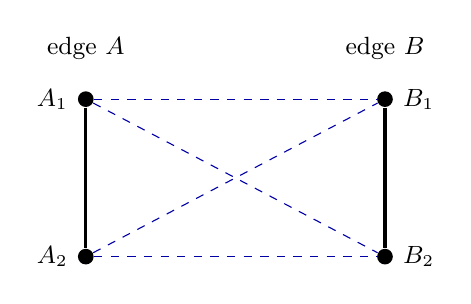
\begin{tikzpicture}[scale=1.0,every node/.style={font=\small}]
\node[circle,fill=black,inner sep=2pt,label=left:\(A_1\)] (a1) at (0,1) {};
\node[circle,fill=black,inner sep=2pt,label=left:\(A_2\)] (a2) at (0,-1) {};
\node[circle,fill=black,inner sep=2pt,label=right:\(B_1\)] (b1) at (3.8,1) {};
\node[circle,fill=black,inner sep=2pt,label=right:\(B_2\)] (b2) at (3.8,-1) {};
\draw[very thick] (a1)--(a2);
\draw[very thick] (b1)--(b2);
\foreach \x in {a1,a2} \foreach \y in {b1,b2}
  \draw[dashed,blue!65!black] (\x)--(\y);
\node at (0,1.65) {edge \(A\)};
\node at (3.8,1.65) {edge \(B\)};
\end{tikzpicture}
\caption{A conflict: solid segments are graph edges, and dashed
segments are holes. The construction forces such a configuration
between different classes of a large matching.}
\label{fig:four-holes}
\end{figure}

For a positive integer \(s\), the \emph{clique blow-up} \(H[s]\)
replaces each vertex of \(H\) by a clique of size \(s\), and each
edge by all edges between the two corresponding cliques.
We also write \(H[K_s]\) for \(H[s]\). An independent set in \(H[s]\) uses at most one vertex from each clique
and projects to an independent set in \(H\). Hence
\(\alpha(H[s])\le2\), and \(\chi(H[s])\ge\lceil ms/2\rceil\).

\Cref{thm:matrix-obstruction} proves that, when \(a\) is fixed,
\(\beta\) is sufficiently small, and \(m\) is sufficiently large,
properties \ref{item:base-colours}--\ref{item:base-holes} force every
well-signed one-negative matrix on \(H[s]\) to have rank greater than
\(ms/2+1\), for every sufficiently large \(s\).
Choosing one base graph from \Cref{thm:base-graphs} and applying
rank--nullity therefore proves \Cref{thm:main}. Notice the order:
the base graph is fixed before the blow-up parameter tends to
infinity.

The independence-number estimate also yields a stronger
fractional-colouring consequence. For a finite nonempty simple graph
\(G\), let \(\mathcal I(G)\) be the family of its independent vertex
sets. A fractional colouring assigns nonnegative real weights \(w_I\)
to these sets with \(\sum_{I\ni v}w_I\ge1\) at every vertex \(v\).
The ordinary fractional chromatic number \(\chi_f(G)\) is the minimum
of \(\sum_Iw_I\) over all such assignments. An ordinary colouring is
a feasible assignment with unit weights on its colour classes, so
\(\chi_f(G)\le\chi(G)\). On the other hand, summing the vertex
constraints gives
\[
 |V(G)|\le \sum_{v\in V(G)}\sum_{I\ni v}w_I
 =\sum_{I\in\mathcal I(G)}|I|w_I
 \le \alpha(G)\sum_{I\in\mathcal I(G)}w_I,
\]
and therefore \(\chi_f(G)\ge |V(G)|/\alpha(G)\).

\begin{corollary}[Fractional-colouring obstruction]\label{cor:fractional-spectral}
There are finite nonempty simple graphs \(G\) of arbitrarily large
order for which
\[
 \chi_f(G)\ge \frac{|V(G)|}{\alpha(G)}
 \ge \frac{|V(G)|}{2}
 >\kappa(G)+1\ge\mu(G)+1\ge h(G).
\]
\end{corollary}
\begin{proof}
Take the constructed examples in Theorem~\ref{thm:main} and put
\(m=|V(G)|\). They have \(\alpha(G)\le2\). Every well-signed
one-negative matrix on these graphs has rank greater than \(m/2+1\),
so rank--nullity gives corank less than \(m/2-1\). Maximizing in the
larger matrix class yields \(\kappa(G)+1<m/2\).
Every matrix admitted in the definition of
\(\mu(G)\) is admitted for \(\kappa(G)\), so \(\mu(G)\le\kappa(G)\).
The inequality \(h(G)\le\mu(G)+1\) was established above. Combining
these bounds with the fractional-colouring estimate proves the chain.
\end{proof}

The same graphs also violate the fractional-colouring weakening
of Hadwiger's conjecture discussed by
\citet[p.~148]{reedseymour1998}: for every positive integer \(p\),
excluding a \(K_{p+1}\) minor was predicted to give a fractional
\(p\)-colouring. Their definition uses nonnegative rational weights
with coverage exactly one at each vertex and total weight at most
\(p\), which are admissible above; their result (1.3) proves the
corresponding \(2p\)-bound.
Taking \(p=h(G)\ge1\) in the corollary rules out the coefficient-one
prediction. The fractional relaxation here concerns colouring,
while \(h(G)\) remains the ordinary clique-minor number. The
comparisons with \(\kappa\) and \(\mu\) show that the obstruction
survives both fractional colouring and omission of the Strong Arnold
Property.

The list chromatic number \(\chi_{\mathrm{list}}(G)\) is the least
integer \(k\) such that every assignment of finite colour lists of
size at least \(k\) to the vertices admits a proper colouring from
those lists.

\begin{corollary}[A linear list-colouring bound]\label{cor:list-spectral}
Let \(C\) be the absolute integer in
\citet[Theorem~1.1]{OpenAILinearListHadwiger2026}. Every finite nonempty
simple graph \(G\) satisfies
\[
 \chi_{\mathrm{list}}(G)\le C\bigl(\mu(G)+1\bigr).
\]
\end{corollary}
\begin{proof}
That theorem gives \(\chi_{\mathrm{list}}(G)\le Ch(G)\). Combining this
with \(h(G)\le\mu(G)+1\), proved above, gives the result.
\end{proof}

\subsection{From distribution tests to finite graphs}

To prove \Cref{thm:base-graphs}, we first work with probability laws
on the finite set of frames. An ordered pair with no hole is called
a \emph{unit}. The two frames within a unit may be strongly dependent.
The tests in \Cref{thm:distribution-tests} give a positive lower bound
for the probability that two independently sampled units conflict
across distinct colours, and that a unit conflicts with an independently
sampled point, under specified density bounds and, in the coloured
test, an upper bound on each colour's mass.

The algebraic part gives sufficient certificates for four cross holes,
using scalar conditions and equalities between ordered tuples of frame images, called
\emph{keys}. Once these equalities and scalar conditions hold,
\Cref{thm:gradient-realization} prescribes the remaining inner products
between primal and channel frames, and \Cref{prop:collision} bounds
the probability of agreement with that prescription. The main
probabilistic task is therefore to force overlap between the accepted
key distributions despite dependence within each unit. Channel thinning
supplies compatible scalar data. The histogram and product comparisons
pass the actual query laws to a common limit, where finite-dimensional
duality produces overlapping choices. Finally, the entropy fingerprint
argument transfers the two distribution tests to one finite sample
satisfying all three base-graph properties.

The paper first proves the matrix criterion. It then constructs
the base graphs. \Cref{sec:geometry,sec:distributions} define the
frame model and thinned law and formulate the distribution tests.
\Cref{sec:moments,sec:realization,sec:collision} supply the finite
algebraic certificates and the collision criterion.
\Cref{sec:phases,sec:preparation} establish compatibility on positive
mass. \Cref{sec:histograms,sec:product-tests,sec:common-limit,sec:status-span}
prove the comparison and overlap statements that establish the
coloured distribution test. \Cref{sec:asymmetric} proves the
independent-point distribution test. \Cref{sec:graph-transfer}
transfers both tests to finite graphs, proving \Cref{thm:base-graphs},
and \Cref{sec:parameters} records the parameter order and quantitative
margins. \Cref{sec:measure-constructions} gives the compact measure
constructions used in the limiting steps.

In the probabilistic construction, \(n\) is its unbounded input
dimension, \(N=M_0n\) is the ambient frame dimension, and
\(m=2^{1000gN}\) is the sampled graph order. The graph threshold
\(\beta\) is distinct from the selector length \(b\).
The original raw probability law is denoted by \(\rawlaw\), and its
thinned version by \(\pi\); \(\mu\) always denotes the graph invariant.

\section{Finite trees for Lorentz blocks}\label{mt:section}

The matrix argument needs a way to normalize several positive definite
blocks at once, even when their dimensions tend to infinity.  We first
give a geometric construction whose constants depend only on the number
of blocks.  We then use the three conflict properties of
\Cref{thm:base-graphs} to select the blocks that will be normalized
together.  All vector spaces and bilinear forms in this section are real.
Logarithms in the hyperbolic estimates are natural logarithms.

\subsection{Hyperbolic flats and block normalization}

A \emph{Lorentz space} is a finite-dimensional real vector space with
bilinear form
\[
 [x,y]=-x_0y_0+\sum_{j=1}^d x_jy_j.
\]
Its future unit hyperboloid is
\[
 \mathbb H^d=\{x:[x,x]=-1,\ x_0>0\},
 \qquad d_{\mathbb H}(x,y)=\operatorname{arcosh}(-[x,y]).
\]
Unused positive coordinates may always be added, so we may take
\(d\ge1\).  The orthogonal complement of a future unit vector is positive
definite.  Indeed, if \(x=(x_0,u)\) and \([x,(t,v)]=0\), then
\(t=u\cdot v/x_0\), and
\[
 |v|^2-t^2\ge |v|^2/x_0^2.
\]
An orthonormal basis of this complement, together with \(x\), therefore
gives Lorentz coordinates in which \(x=(1,0)\).  In these coordinates any
other future unit vector has the form
\((\cosh r,\sinh r\,u)\), with \(|u|=1\) and \(r\ge0\).
In particular \(-[x,y]\ge1\).  If \(y,z\) have radii \(r,s\) about
\(x\), the ordinary Cauchy--Schwarz inequality gives
\[
 -[y,z]=\cosh r\cosh s-\sinh r\sinh s\,(u\cdot v)
 \le \cosh(r+s).
\]
This proves the triangle inequality for \(d_{\mathbb H}\); its other
metric properties follow from the same coordinates.

The segment from \(x\) to \(y\), of length \(\ell>0\), is
\begin{equation}\label{mt:hyperbolic-segment}
 \gamma(t)=\frac{\sinh(\ell-t)}{\sinh\ell}x
            +\frac{\sinh t}{\sinh\ell}y,
 \qquad 0\le t\le\ell.
\end{equation}
In coordinates about \(x\) it is \((\cosh t,\sinh t\,u)\), so
\(d_{\mathbb H}(\gamma(t),\gamma(t'))=|t-t'|\).
When \(x=y\) the segment is constant.  A subspace \(P\) is
\emph{positive} if the Lorentz form restricted to it is positive
definite.  Its associated \emph{flat} is
\[
 F_P=P^\perp\cap\mathbb H^d.
\]
Orthogonal decomposition by a positive subspace leaves exactly one
negative square, so \(F_P\) is nonempty.  Formula
\eqref{mt:hyperbolic-segment} shows that it contains the segment between
any two of its points.

\begin{lemma}[Normalization near a flat]\label{mt:flat-normalization}
Let \(P\) be positive and write \(x=x_P+x_\perp\) for the orthogonal
decomposition of \(x\in\mathbb H^d\) relative to \(P\).  Then
\begin{equation}\label{mt:flat-distance}
 \sinh^2 d_{\mathbb H}(x,F_P)=[x_P,x_P].
\end{equation}
Suppose \(P_1,\ldots,P_k\) are positive subspaces whose flats have
distance at most \(R\) from one common point.  Choose any
Lorentz-orthonormal basis in each \(P_i\), concatenate these bases into
a list \(A\), and let \([A,A]\) be its Gram matrix.  Then
\begin{equation}\label{mt:block-operator-bound}
 \|[A,A]\|_{\mathrm{op}}
 \le k(\cosh^2R+\sinh^2R).
\end{equation}
This bound does not depend on the dimensions of the subspaces.  The
subspaces are allowed to overlap.  If \(P_i\perp P_j\), then
\(F_{P_i}\cap F_{P_j}\ne\varnothing\).
\end{lemma}
\begin{proof}
Put \(q=[x_P,x_P]\).  Then \([x_\perp,x_\perp]=-1-q\), and
\(y=x_\perp/\sqrt{1+q}\) is future unit timelike.  For \(z\in F_P\),
the hyperbolic coordinates above, now in \(P^\perp\), give
\[
 -[x,z]=-[x_\perp,z]\ge\sqrt{1+q},
\]
with equality at \(z=y\).  This proves \eqref{mt:flat-distance}.

Use the common point as the time coordinate.  For the basis matrix
\(A_i\), let \(t_i\) be its time-coordinate row and \(S_i\) its
spatial-coordinate matrix.  The projection formula gives
\(\|t_i\|\le\sinh R\), and orthonormality gives
\[
 S_i^{\mathsf T}S_i=I+t_i^{\mathsf T}t_i,
 \qquad \|S_i\|_{\mathrm{op}}\le\cosh R.
\]
For the concatenated matrices \(S,t\), Cauchy--Schwarz over the \(k\)
blocks gives \(\|S\|_{\mathrm{op}}^2\le k\cosh^2R\) and
\(\|t\|^2\le k\sinh^2R\).  Since
\([A,A]=S^{\mathsf T}S-t^{\mathsf T}t\), this proves
\eqref{mt:block-operator-bound}.  Finally, if \(P_i\perp P_j\), their
sum is positive, and its orthogonal complement contains a future unit
timelike vector perpendicular to both.
\end{proof}

\subsection{A finite configuration and its segment points}

A \emph{finite metric tree} is a finite tree whose edges are intervals
of positive lengths, equipped with path distance; a single point is
also allowed.  Its segment between \(a,b\) is denoted \([a,b]_T\).

Finite hyperbolic configurations admit tree approximations with
logarithmic additive error through Gromov's construction
\citep{Gromov1987Hyperbolic}. Its maximum--minimum chain closure is
recorded explicitly by \citet[Section~2, equation~(11)]{CornectMartinezPedroza2025Tree}.
We give a direct hyperboloid argument with an error depending only on
the number of marked points; the subsequent segment and flat lemmas
supply the additional assertions needed for matrix normalization.

\begin{lemma}[Finite tree approximation]\label{mt:finite-metric}
For \(\ell\ge1\), put
\[
 K(\ell)=4+2\log\bigl(\max\{1,\ell-1\}\bigr).
\]
Given any \(\ell\) points \(z_1,\ldots,z_\ell\) in a hyperboloid, in any
dimension, there is a finite metric tree with marked points
\(z_1^T,\ldots,z_\ell^T\) such that
\begin{equation}\label{mt:endpoint-error}
 \bigl|d_T(z_i^T,z_j^T)-d_{\mathbb H}(z_i,z_j)\bigr|\le K(\ell).
\end{equation}
The tree may be taken to be the hull of its marked points.
\end{lemma}
\begin{proof}
Take \(z_1\) as origin and write
\(z_i=(\cosh r_i,\sinh r_i\,u_i)\).  A direction with \(r_i=0\)
can be chosen arbitrarily.  For distinct indices set
\[
 q_{ij}=\frac{|u_i-u_j|}{2},\qquad
 a_{ij}=\min\{r_i,r_j,-\log q_{ij}\},
\]
with \(-\log0=+\infty\), and set \(a_{ii}=r_i\).  The exact identity
\begin{equation}\label{mt:radial-identity}
 \cosh d_{\mathbb H}(z_i,z_j)
 =\cosh(r_i-r_j)+2\sinh r_i\sinh r_j\,q_{ij}^2
\end{equation}
implies
\begin{equation}\label{mt:raw-depth-error}
 \left|d_{\mathbb H}(z_i,z_j)-(r_i+r_j-2a_{ij})\right|\le4.
\end{equation}
Here is a dimension-free verification.  If \(\min(r_i,r_j)<1\),
the triangle inequality and its reverse put both
\((r_i+r_j-d_{\mathbb H}(z_i,z_j))/2\) and \(a_{ij}\) between zero
and \(\min(r_i,r_j)\), giving error at most two.  Otherwise, writing
\[
 D=\max\{|r_i-r_j|,\ r_i+r_j+2\log q_{ij}\}
   =r_i+r_j-2a_{ij},
\]
the two terms in \eqref{mt:radial-identity} give
\(e^D/4\le\cosh d_{\mathbb H}(z_i,z_j)\le2e^D\).
Use \(\log u\le\operatorname{arcosh}u\le\log(2u)\) for \(u\ge1\)
to obtain an error at most \(\log4<4\).

For \(i\ne j\), define \(A_{ij}\) as the largest bottleneck value
\(\min_{0\le t<k}a_{i_ti_{t+1}}\) over chains
\(i=i_0,\ldots,i_k=j\), and put \(A_{ii}=r_i\).
Deleting loops never decreases a bottleneck, so only simple chains
of at most \(\ell-1\) edges are needed.  If a chain has bottleneck \(h\),
its endpoint radii are at least \(h\), and the triangle inequality
for the direction chords gives
\(q_{ij}\le(\ell-1)e^{-h}\).  Consequently
\begin{equation}\label{mt:bottleneck-bound}
 a_{ij}\le A_{ij}
 \le a_{ij}+\log\bigl(\max\{1,\ell-1\}\bigr),\qquad
 A_{ij}\le\min(r_i,r_j).
\end{equation}
Concatenating chains also gives
\(A_{ij}\ge\min(A_{it},A_{tj})\) for every \(t\).
Take intervals \([0,r_i]\), identifying their points of equal height
\(t\) whenever \(t\le A_{ij}\).  The last inequality makes this an
equivalence relation at every height.  These equivalence classes are
nested as height decreases; their finitely many splitting heights
therefore form a rooted finite tree.  The distance between the two
marked upper endpoints is
\(r_i+r_j-2A_{ij}\).  Equations
\eqref{mt:raw-depth-error}--\eqref{mt:bottleneck-bound} prove
\eqref{mt:endpoint-error}.  Restricting to the hull of the marked
points preserves their distances.
\end{proof}

Endpoint approximation alone does not justify lifting a point of a
tree hull back into a flat.  The next lemma supplies this additional
step, uniformly in the location of the point along its segment.

\begin{lemma}[Comparison of segment points]\label{mt:segment-comparison}
Let \(T\) and the points \(z_i^T\) satisfy
\eqref{mt:endpoint-error}.  For \(\theta\in[0,1]\), associate the
point at fraction \(\theta\) of \([z_i^T,z_j^T]_T\) with the point
at the same fraction of the hyperbolic segment \([z_i,z_j]\).
If \(p,q\) are obtained in this way, from any two pairs of marked
points, and \(\widehat p,\widehat q\) are their associated hyperbolic
points, then
\begin{equation}\label{mt:segment-error}
 \bigl|d_{\mathbb H}(\widehat p,\widehat q)-d_T(p,q)\bigr|
 \le 11K(\ell+2).
\end{equation}
For a degenerate segment any choice of its fractional parameter gives
the same conclusion.
\end{lemma}
\begin{proof}
We first record an identity valid in any metric tree.  If
\(p\in[a,b]_T\) and \(q\in[c,d]_T\), then
\begin{equation}\label{mt:tree-segment-identity}
 d_T(p,q)=\max_{e\in\{a,b\},\ f\in\{c,d\}}
 \{d_T(e,f)-d_T(e,p)-d_T(f,q)\}.
\end{equation}
Every term is at most the left side by the triangle inequality.
If \(p\ne q\), choose an endpoint \(e\) whose path from \(p\)
does not enter the component toward \(q\), and an endpoint \(f\)
whose path from \(q\) does not enter the component toward \(p\).
Such choices exist because \(p,q\) lie on their respective segments;
an endpoint equal to the segment point is allowed.  Then the path
from \(e\) to \(f\) passes through \(p,q\), giving equality.  If
\(p=q\), either choose an endpoint equal to this common point, or
choose endpoints in different components of its complement; again
equality holds.

A second exact tree identity will locate the new marked points.
If $P_\theta$ is at fraction $\theta$ of $[A,B]$ and $X$ is any
point of the tree, then
\begin{equation}\label{mt:tree-point-identity}
 d(X,P_\theta)=\max\{d(A,X)-\theta d(A,B),\,
                     d(B,X)-(1-\theta)d(A,B)\}.
\end{equation}
Indeed, if the projection of $X$ onto $[A,B]$ is at distance $u$
from $A$ and at distance $h$ from $X$, both sides equal
$h+|u-\theta d(A,B)|$.  This also holds for a degenerate segment.

Apply \Cref{mt:finite-metric} to the original configuration together
with $\widehat p,\widehat q$, obtaining a tree $T'$ with error
$K'=K(\ell+2)$.  Denote their marked points by $p',q'$.  Suppose
$\widehat p$ is at fraction $\theta$ of the hyperbolic segment
$[a,b]$, and let $\widetilde p$ have that fraction on
$[a',b']_{T'}$.  The two exact hyperbolic distances from $\widehat p$
to its endpoints are $\theta d_{\mathbb H}(a,b)$ and
$(1-\theta)d_{\mathbb H}(a,b)$.  In
\eqref{mt:tree-point-identity}, each corresponding difference is
therefore at most $2K'$.  Thus
\[
 d_{T'}(p',\widetilde p)\le2K',\qquad
 d_{T'}(q',\widetilde q)\le2K'.
\]
Together with the $K'$ distance error for the pair
$\widehat p,\widehat q$, this gives
\[
 |d_{\mathbb H}(\widehat p,\widehat q)
       -d_{T'}(\widetilde p,\widetilde q)|\le5K'.
\]
Between the original endpoint sets, distances in $T$ and $T'$
differ by at most $K(\ell)+K'\le2K'$.  Distances from an endpoint
to its fractional segment point are that fraction, or its complement,
times the segment length.  Each term in
\eqref{mt:tree-segment-identity} therefore changes by at most
$6K'$, and hence
\[
 |d_T(p,q)-d_{T'}(\widetilde p,\widetilde q)|\le6K'.
\]
The total error is at most $11K'$.  All identities remain valid when
an endpoint segment has length zero.
\end{proof}

\begin{proposition}[Finite tree principle]\label{mt:finite-tree}
For each index \(s\), let \(P_{1,s},\ldots,P_{k,s}\) be positive
subspaces in a Lorentz space, whose dimension may depend on \(s\).
Fix a set \(\mathcal D\) of pairs of distinct labels, and assume
\[
 \sup_s d_{\mathbb H}(F_{P_{i,s}},F_{P_{j,s}})\le D<\infty
 \qquad (\{i,j\}\in\mathcal D).
\]
After passing to a subsequence, there are a finite combinatorial tree
\(T\) and a nonempty connected vertex set \(S_i\subseteq V(T)\)
for every label, with the following properties.
\begin{enumerate}[label=\textup{(\roman*)}]
\item \(S_i\cap S_j\ne\varnothing\) for every
\(\{i,j\}\in\mathcal D\).
\item For every vertex \(x\), called a \emph{bag}, choose any
Lorentz-orthonormal basis in every \(P_{i,s}\) with \(x\in S_i\).
The Gram matrix of the concatenated list has operator norm bounded
uniformly in \(s\).  The bound depends only on \(k,D\), and not on
the dimensions or on the bases.
\end{enumerate}
In particular, mutually orthogonal blocks can always be required to
have intersecting subtrees.
\end{proposition}
\begin{proof}
For every required pair, choose a point in each of its two flats at
distance at most \(D+1\); an infimum need not be attained.  Choose
also one point in each flat.  This gives
\(\ell=k+2|\mathcal D|\le k^2\) marked representatives.  Apply
\Cref{mt:finite-metric} and work in their tree hull \(K_s\).
Let \(H_{i,s}\) be the hull of representatives chosen from the
\(i\)-th flat, and set
\[
 R=\frac{D+1+K(\ell)}2,\qquad
 U_{i,s}=\{x\in K_s:d_T(x,H_{i,s})\le R\}.
\]
The \(R\)-neighborhood of a subtree in a tree is a closed subtree: the
segment between two of its points lies in the union of their paths
to the original subtree and the subtree itself, and stays within
distance \(R\) of it.
For a required pair, the midpoint of its two witness representatives
belongs to both neighborhoods.  Thus every required contact is
preserved inside \(K_s\).

Suppose \(x\in U_{i,s}\cap U_{j,s}\).  Choose
\(h_i\in H_{i,s}\), \(h_j\in H_{j,s}\) at distance at most \(R\)
from \(x\).  Every point of a finite tree hull lies on a segment
between two of its defining representatives, allowing a repeated
representative when the hull is a point.  For example, after fixing
one representative the union of its segments to all the others is
already their hull.  Lift \(h_i,h_j\) at their fractional parameters
along the corresponding actual hyperbolic segments.  Their lifts
\(z_i,z_j\) belong to their respective flats by convexity, and
\Cref{mt:segment-comparison} gives
\begin{equation}\label{mt:bag-radius}
 d_{\mathbb H}(z_i,z_j)\le 2R+11K(\ell+2)=:R_*.
\end{equation}
For any nonempty bag, fix one of these lifts.  It has distance at
most \(R_*\) from every flat in the bag.  By
\Cref{mt:flat-normalization}, their joint Gram norm is at most
\(k(\cosh^2R_*+\sinh^2R_*)\).

It remains to obtain a single finite combinatorial pattern.  Suppress
the degree-two vertices of \(K_s\) except marked representatives;
there are at most \(2\ell\) vertices and at most \(2\ell\) edges.
Each \(U_{i,s}\) meets an edge in an interval or the empty set.
Subdivide every edge at all endpoints of these intervals.  This
adds at most \(2k\) vertices per edge, so the resulting tree has at
most \(2\ell(2k+1)\) vertices.  Each \(U_{i,s}\) is now a subcomplex.
There are only finitely many trees of this bounded size with \(k\)
specified nonempty connected vertex sets.  Along a subsequence the
labelled pattern is constant.  Take this pattern for \(T,S_i\).
Equation \eqref{mt:bag-radius} proves the uniform bag assertion.
The final assertion follows from \Cref{mt:flat-normalization} with
\(D=0\).
\end{proof}

For a finite list of flat sequences, a preliminary subsequence can
also arrange that every pairwise distance is either uniformly bounded
or tends to infinity.  For each pair in turn, take a bounded subsequence
if one exists, and otherwise the distance tends to infinity; previous
choices remain valid after further subselection.  Applying
\Cref{mt:finite-tree} with all bounded pairs as required contacts
preserves every such pair.  No assertion that the remaining subtrees
are disjoint is needed.

\subsection{Weighted extraction from the conflict properties}

We use a finite graph \(G\) on \(m\) vertices with the three
properties in \Cref{thm:base-graphs}, with parameters \(a,\beta>0\).
For clarity, the properties used here are:
\begin{enumerate}[label=\textup{(\alph*)}]
\item\label{mt:property-colour}
Every matching of size at least \(m/20\), partitioned into classes
of size at most \(am\), contains conflicting edges from different
classes.
\item\label{mt:property-point}
Every matching of size at least \(\beta m\) and every vertex set of
size at least \(\beta m\) contain an edge and a vertex in conflict.
\item\label{mt:property-hole}
Every two vertex sets of size at least \(\beta m\) have a cross hole.
\end{enumerate}
A hole is a nonedge between distinct vertices.  Edges conflict when
they are disjoint and all four cross pairs are holes.  An edge and a
vertex conflict when the vertex is outside the edge and both cross
pairs are holes.  Thus a shared endpoint prevents a conflict.
We may decrease \(a\) and assume \(0<a\le1\).  Put
\begin{equation}\label{mt:constants}
 q=\lceil\beta m\rceil,\qquad
 D_a=\lceil\log_2(5/a)\rceil+1,\qquad
 K_a=\lceil5/a\rceil D_a,\qquad
 c=c(a)=\frac1{40K_a}.
\end{equation}

An edge family \(\mathcal E\subseteq E(G)\) has \emph{loads at most
one} if its nonnegative weights satisfy
\begin{equation}\label{mt:loads}
 \sum_{e\in\mathcal E:\,v\in e}w_e\le1
 \qquad(v\in V(G)).
\end{equation}
Then \(\sum_e w_e\le m/2\).  We only need edges of positive weight.

\begin{lemma}[Matching from bounded loads]\label{mt:load-matching}
Every edge family of total weight \(W\) satisfying
\eqref{mt:loads} has a matching of size at least \(W/2\).
If it contains no conflicting pair and \(am\ge1\), then
\(W<m/10\).
\end{lemma}
\begin{proof}
Take a maximal matching of size \(k\) in the family.  Its \(2k\)
endpoints cover every edge, so the load bound gives \(W\le2k\).
In the second assertion, \(k\ge m/20\) would violate
Property~\ref{mt:property-colour} with each matching edge given its
own class.  Hence \(k<m/20\), proving the claim.
\end{proof}

\begin{lemma}[A bag with almost all vertex labels]\label{mt:single-bag}
Let \(V_0\subseteq V(G)\), and assign a nonempty subtree
\(S_v\) of a finite combinatorial tree to each \(v\in V_0\).
Assume \(S_u\cap S_v\ne\varnothing\) whenever \(uv\) is a hole.
Then some tree vertex belongs to all but fewer than \(3q\) of the
subtrees.
\end{lemma}
\begin{proof}
At a tree vertex \(x\), each subtree missing \(x\) is wholly
contained in a unique component of \(T-x\).  No two components
can each contain at least \(q\) whole subtrees: taking \(q\) labels
from each would give two vertex sets with no cross hole, contrary
to Property~\ref{mt:property-hole}.  If there is a component with
at least \(q\) whole subtrees, orient the first edge from \(x\)
toward that component.  Each vertex has at most one outgoing edge.
An edge cannot be oriented both ways, since its two orientations
would again supply two separated sets of \(q\) labels.  Following
arrows in a finite tree must therefore end at a sink \(r\).

Every component of \(T-r\) contains at most \(q-1\) whole
subtrees.  If \(q=1\), no subtree misses \(r\).  If \(q\ge2\)
and at least \(3q-2\) labels missed \(r\), greedily unite components
until their total first reaches \(q\).  This total is at most
\(2q-2\); the remaining components contain at least \(q\) labels.
These two separated families contradict
Property~\ref{mt:property-hole}.  The sink thus misses fewer than
\(3q-2\), and in particular fewer than \(3q\), labels.
\end{proof}

\begin{lemma}[A bag with positive edge weight]\label{mt:weighted-bag}
Suppose \(am\ge2\).  Let an edge family \(\mathcal E\) satisfy
\eqref{mt:loads} and have total weight greater than \(3m/10\).
Assign a nonempty subtree \(S_e\) of a finite tree to each edge,
and suppose conflicting edges have intersecting subtrees.
Then some vertex \(z\) satisfies
\[
 \sum_{e:\,z\in S_e}w_e\ge cm.
\]
\end{lemma}
\begin{proof}
Assign every edge's weight to one chosen vertex of its subtree.
Every finite tree with an assigned nonnegative mass has a vertex
whose removal leaves each component with at most half the total
mass.  To see this, minimize the sum of mass times graph distance
from the vertex.  Moving to a neighbor in a component of mass
greater than half the total would strictly decrease that sum.
Such a minimizing vertex is a weighted centroid.

Starting with \(T\), cut at a weighted centroid in every current
component whose assigned mass exceeds \(am/10\), and repeat.
At depth \(j\) each component has mass at most \(m/2^{j+1}\),
since the original mass is at most \(m/2\).  Consequently at most
\(D_a\) rounds are needed.  At each depth there are at most
\(\lceil5/a\rceil\) components requiring a cut, because their
masses sum to at most \(m/2\).  Thus at most \(K_a\) cut vertices
are used.  Mass located at a cut vertex is removed at that cut.

Suppose every bag has edge weight less than \(cm\).  Delete every
edge whose subtree meets a cut vertex.  The deleted weight is less
than \(K_acm=m/40\), so the surviving weight \(W'\) satisfies
\(W'>m/4\).  Each surviving subtree is wholly contained in one
component of the cut tree; its assigned vertex lies there too.
The total surviving weight in each such component is at most
\(am/10\).  Use the components as classes of surviving edges.
Subtrees of different classes are disjoint, so edges in different
classes cannot conflict.

Put \(Q=\lfloor am\rfloor\), so \(Q\ge am/2\).  Greedily choose
a matching, with at most \(Q\) selected edges from any class,
until no further edge can be added.  If \(k\) edges have been
selected, every surviving edge either meets one of their \(2k\)
endpoints or belongs to a class with \(Q\) selected edges.  The
first family has weight at most \(2k\).  There are at most
\(k/Q\) saturated classes, each of weight at most \(am/10\).
Therefore
\[
 \frac m4<W'\le 2k+\frac{k}{Q}\frac{am}{10}
 \le\frac{11}{5}k.
\]
It follows that \(k>5m/44>m/20\).  Its class sizes are at most
\(Q\le am\), but it has no conflict between different classes.
This contradicts Property~\ref{mt:property-colour}.
\end{proof}

\begin{proposition}[A common bag]\label{mt:common-bag}
Suppose the hypotheses of \Cref{mt:single-bag,mt:weighted-bag}
hold in the same tree.  Suppose additionally that
\(S_e\cap S_v\ne\varnothing\) whenever the edge \(e\) and the
vertex \(v\in V_0\) conflict.  If
\(q\le cm/4\), there is a vertex \(x\) such that
\begin{equation}\label{mt:common-counts}
 |\{v\in V_0:x\notin S_v\}|<5q,
 \qquad \sum_{e:\,x\in S_e}w_e\ge\frac{cm}{2}.
\end{equation}
If all edges of \(\mathcal E\) have both endpoints in \(V_0\) and
\(q\le cm/30\), deleting every edge incident with a missing vertex
leaves bag weight at least \(cm/3\).
\end{proposition}
\begin{proof}
Let \(r\) be the vertex bag from \Cref{mt:single-bag}, let
\(z\) be the edge bag from \Cref{mt:weighted-bag}, and let
\(A=\{v\in V_0:r\in S_v\}\).  Along the path from \(r\) to
\(z\), each \(S_v\) with \(v\in A\) is an initial interval.
Thus the number of absent labels from \(A\) is nondecreasing.
If fewer than \(2q\) are absent at \(z\), use \(x=z\).
It misses fewer than \(3q+2q\) supplied vertex labels and has
edge weight at least \(cm\).

Otherwise let \(xy\) be the first edge of this path, in the
direction from \(r\) to \(z\), for which fewer than \(2q\)
labels of \(A\) are absent at \(x\), and at least \(2q\) are
absent at \(y\).  Set
\[
 A_- =\{v\in A:y\notin S_v\},\qquad
 \mathcal E_+=\{e:z\in S_e,\ x\notin S_e\}.
\]
Every subtree indexed by \(A_-\) is contained in the \(x\)-side
of \(T-xy\): it contains \(r\) and avoids \(y\).  Every subtree
indexed by \(\mathcal E_+\) is contained in the \(y\)-side: it
contains \(z\) and avoids \(x\).  In particular these two
families are disjoint.  This uses \emph{all} root labels absent at
\(y\), including labels that ceased to occur earlier on the path;
it does not require many labels to disappear on the single edge
\(xy\).  See \Cref{mt:fig-path}.

If the bag weight at \(x\) were less than \(cm/2\), then
\(\sum_{e\in\mathcal E_+}w_e>cm/2\).
By \Cref{mt:load-matching}, \(\mathcal E_+\) has a matching of
size greater than \(cm/4\), hence at least \(q\) since
\(q\le cm/4\).  Also \(|A_-|\ge2q\).  No selected edge conflicts
with any label in \(A_-\), because such a conflict would force
intersecting subtrees.  Taking any \(q\) of these labels violates
Property~\ref{mt:property-point}.  Thus the bag at \(x\) has weight
at least \(cm/2\); it misses fewer than \(5q\) supplied labels.

Finally, the load bound shows that removing all edges incident
with these missing vertices costs less than \(5q\) weight.
If \(q\le cm/30\), the surviving bag weight is at least
\(cm/2-5q\ge cm/3\), as asserted.
\end{proof}

\begin{figure}[htbp]
\centering
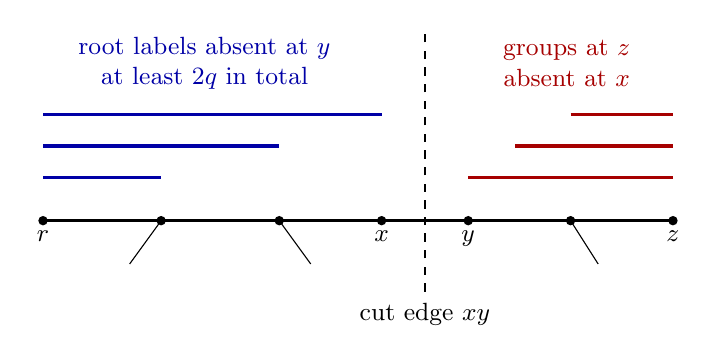
\begin{tikzpicture}[x=1cm,y=1cm,every node/.style={font=\small}]
\draw[very thick] (0,0)--(8,0);
\foreach \x in {0,1.5,3,4.3,5.4,6.7,8}
  \fill (\x,0) circle (1.7pt);
\draw (1.5,0)--(1.1,-.55);
\draw (3,0)--(3.4,-.55);
\draw (6.7,0)--(7.05,-.55);
\node[below] at (0,0) {$r$};
\node[below] at (4.3,0) {$x$};
\node[below] at (5.4,0) {$y$};
\node[below] at (8,0) {$z$};
\draw[dashed,thick] (4.85,-.9)--(4.85,2.4);
\node[below,align=center] at (4.85,-.92) {cut edge $xy$};
\draw[blue!65!black,very thick] (0,.55)--(1.5,.55);
\draw[blue!65!black,very thick] (0,.95)--(3,.95);
\draw[blue!65!black,very thick] (0,1.35)--(4.3,1.35);
\node[blue!65!black,align=center] at (2.05,2.0)
 {root labels absent at $y$\\at least $2q$ in total};
\draw[red!65!black,very thick] (5.4,.55)--(8,.55);
\draw[red!65!black,very thick] (6.0,.95)--(8,.95);
\draw[red!65!black,very thick] (6.7,1.35)--(8,1.35);
\node[red!65!black,align=center] at (6.65,2.0)
 {groups at $z$\\absent at $x$};
\end{tikzpicture}
\caption{The path argument uses cumulative absence.  The blue intervals
show intersections with the path of root subtrees that avoid \(y\);
some may end well before \(x\).  The red intervals come from group
subtrees containing \(z\) and avoiding \(x\).  The two whole families
lie on opposite sides of the cut, so no edge--vertex conflict can
occur between them.}
\label{mt:fig-path}
\end{figure}

\begin{remark}[Use with coordinate matchings]\label{mt:coordinate-interface}
In the matrix application a base label indexes at most \(s\)
coordinates, and the edge weight is the limit of the number of matched
coordinate pairs of that type divided by \(s\).  A matching gives
\eqref{mt:loads} automatically.  Deleting all pairs incident with the
fewer than \(5q\) labels missing from the common bag removes fewer
than \(5qs\) pairs.  It removes entire edge types, so any previously
chosen normalization inside a retained type stays the same.
The finite tree principle applies jointly to the original positive
label blocks and the positive blocks of the candidate edge types.
These subspaces may overlap.  A common bag consequently bounds all
their normalized Gram interactions at once.  Passing to coordinate
subsets is a compression by an isometry, so it preserves that bound.
\end{remark}

\section{The matrix obstruction}\label{mr:section}

We now prove the conditional matrix statement.  Only the three
properties of the base graph enter this section; the Strong Arnold
Property is not needed.  Throughout, $v=ms$ denotes the order of the
clique blow-up.  Matrix traces and squared Frobenius norms will be divided
by $v$, even when the matrix under consideration has fewer than $v$
rows.

\begin{theorem}[Matrix obstruction]\label{thm:matrix-obstruction}
For every $a\in(0,1]$ there are constants $\beta_0(a)>0$ and
$m_0(a)\in\mathbb N$ with the following property.  Let
$0<\beta\le\beta_0(a)$, let $m\ge m_0(a)$, and let $G$ be an
$m$-vertex graph satisfying the following conditions:
\begin{enumerate}[label=\textup{(\roman*)}]
\item Every matching of size at least $m/20$, partitioned into classes
of size at most $am$, contains two conflicting edges in different
classes.
\item Every matching of size at least $\beta m$ and every vertex set of
size at least $\beta m$ contain a conflicting edge--point pair.
\item Every two vertex sets of size at least $\beta m$ have a cross hole.
\end{enumerate}
Then there is $s_0=s_0(G,a,\beta)$ such that, for every integer
$s\ge s_0$, every real symmetric well-signed matrix $M$ for the clique
blow-up $G[K_s]$ with exactly one negative eigenvalue satisfies
\[
  \rank M>\frac{ms}{2}+1.
\]
Consequently $\mu(G[K_s])+1<ms/2$ for all these $s$.
\end{theorem}

The proof uses two normalizations.  A first normalization, separately
inside the vertex cliques, produces almost disjoint coordinate pairs.
A second normalization, inside groups of pairs having the same two base
labels, supplies additional positive directions.  The tree lemmas ensure
that both normalizations can be used in one bounded Gram matrix.  We first
give the linear-algebra estimates that make the errors independent of the
bounds furnished by the tree.

\subsection{Positive blocks and bounded spectral limits}

For a real symmetric matrix $A$, write $n_+(A)$ and $n_-(A)$ for its
positive and negative indices, counting multiplicity.  The notation
$\|A\|$ means the Euclidean operator norm, and
$\|A\|_{\mathrm F}^2=\Tr(A^{\mathsf T}A)$.  A symmetric matrix with
at most one negative eigenvalue is a Gram matrix for the Lorentz form
\[
  \langle x,y\rangle=-x_0y_0+\sum_{i\ge1}x_i y_i:
\]
diagonalize the matrix and multiply each eigenvector coordinate by the
square root of the absolute value of its eigenvalue.  Unused positive
coordinates can be added.  Every restriction or coefficient pullback of
this Gram matrix still has at most one negative eigenvalue.  For lists
$X,Y$ of Lorentz vectors, $\langle X,Y\rangle$ denotes their rectangular
Gram matrix; the same letter denotes the corresponding synthesis map.

The next facts are standard consequences of symmetric $M$-matrix
theory and the Perron--Frobenius theorem; see
\citet[Theorem~5.2]{FiedlerSchneider1983Analytic} and
\citet[Theorem~I]{DebreuHerstein1953Nonnegative}.
Here an $M$-matrix has the form $cI-A$ with $A$ entrywise
nonnegative and $c$ at least its spectral radius. We include the
elementary proofs for the precise symmetric cases used below.

\begin{lemma}[Normalization of a positive block]\label{mr:positive-block}
Let $D$ be real symmetric with nonpositive off-diagonal entries.
\begin{enumerate}[label=\textup{(\roman*)}]
\item If $D$ is positive definite, its positive inverse square root
$D^{-1/2}$ is entrywise nonnegative and has positive diagonal entries.
\item Suppose $D$ is positive semidefinite and the graph of its strictly
negative off-diagonal entries is connected.  If $D$ is singular, its
kernel is one-dimensional and is spanned by a vector all of whose
coordinates are positive.  Every proper principal submatrix of $D$ is
positive definite.
\end{enumerate}
\end{lemma}

\begin{proof}
For (i), choose $c>\lambda_{\max}(D)$ and put $A=I-D/c$.
All entries of $A$ are nonnegative, and its eigenvalues lie in $[0,1)$.
The convergent binomial series gives
\begin{equation}\label{mr:inverse-root}
 D^{-1/2}=c^{-1/2}\sum_{k=0}^{\infty}
       \frac{\binom{2k}{k}}{4^k}A^k.
\end{equation}
Every term is entrywise nonnegative, and the constant term has positive
diagonal.

For (ii), take $c>\lambda_{\max}(D)$ and consider $A=cI-D$.
It is symmetric and entrywise nonnegative, with positive diagonal and
connected off-diagonal support.  A unit vector maximizing its Rayleigh
quotient may be replaced by its coordinatewise absolute value, so a
nonnegative maximizing eigenvector exists.  Its eigenvalue is positive.
The eigenvector equation and connectivity imply that it has no zero
coordinate: a zero coordinate would force zeros at every adjacent
coordinate and then everywhere.  Moreover, every vector for the largest
eigenvalue has one sign.  Indeed, equality in the absolute-value
Rayleigh inequality forces equal signs across each positive edge, while
its absolute value is a nonnegative maximizing eigenvector and thus has
full support.  If the largest eigenspace had dimension at least two, it
would contain a nonzero vector orthogonal to the positive eigenvector;
that vector could not have one sign.  The largest eigenvalue is therefore
simple.

When $D$ is singular and positive semidefinite, this largest eigenvalue
of $A$ is $c$, so the asserted kernel description follows.  If a proper
principal submatrix were singular, extend a nonzero vector of zero
quadratic form by zero coordinates.  Its quadratic form under $D$ is
zero, hence it belongs to $\ker D$ by the spectral theorem.  This
contradicts full support.
\end{proof}

\begin{lemma}[Spectral support from signs and inertia]
\label{mr:spectral-support}
Let $v_j\to\infty$, and let $B_j$ be symmetric entrywise nonnegative
matrices of orders $d_j\le v_j$, with zero diagonal and
$\sup_j\|B_j\|<\infty$.  Suppose $n_-(I-B_j)\le1$.
Every weak subsequential limit of
\[
 \nu_j=\frac1{v_j}\sum_{i=1}^{d_j}\delta_{\lambda_i(B_j)}
\]
is supported on $[-1,1]$ and has first moment zero.  In particular, for
each $\varepsilon>0$, the number of eigenvalues of $I-B_j$ outside
$[-\varepsilon,2+\varepsilon]$ is $o(v_j)$.

If also
\[
 \liminf_j\frac{d_j}{v_j}\ge1-\delta,
 \qquad \rank(I-B_j)\le v_j/2+1,
\]
then
\begin{equation}\label{mr:spectral-error}
 \limsup_j\frac{\|B_j^2-I\|_{\mathrm F}^2}{v_j}\le2\delta.
\end{equation}
The constant in this inequality is independent of the operator bound.
\end{lemma}

\begin{proof}
By \Cref{lem:compact-measures}, all measures have bounded mass and support in a common compact interval,
so every subsequence has a weakly convergent further subsequence.  Fix
such a limit $\nu$, and write $\theta=\nu(\mathbb R)\le1$.
At most one eigenvalue of $B_j$ exceeds $1$, hence $\nu$ is supported
on $(-\infty,1]$.  For every integer $k\ge0$, entrywise nonnegativity
gives $\Tr B_j^{2k+1}\ge0$, and therefore
$\int x^{2k+1}\,d\nu(x)\ge0$.  If $\nu$ gave mass $h>0$ to
$(-\infty,-1-\varepsilon]$, this integral would be at most
$\theta-h(1+\varepsilon)^{2k+1}$, which is negative for large $k$.
This proves the support assertion.  The zero diagonal gives
$\int x\,d\nu(x)=0$.  The asserted eigenvalue count follows by applying
these facts to any putative subsequence on which the normalized
exceptional count stays positive.

For the additional assertion, pass to a subsequence realizing the
limsup in \eqref{mr:spectral-error} and then to a weak limit as above.
The nullity assumption supplies at least $d_j-v_j/2-1$ eigenvalues
equal to $1$.  Since singleton sets are closed, weak convergence gives
$r:=\nu(\{1\})\ge\theta-1/2$.  Consequently
\[
 \int_{x\ne1}(1+x)\,d\nu(x)=\theta-2r
       \le1-\theta\le\delta.
\]
For $-1\le x\le1$ we have
$(1-x^2)^2\le1-x^2\le2(1+x)$, and the first expression vanishes at
$x=1$.  Polynomial integrals converge on the common compact support,
so
\[
 \lim_j\frac{\|B_j^2-I\|_{\mathrm F}^2}{v_j}
  =\int(1-x^2)^2\,d\nu(x)\le2\delta.
\]
In this argument the bound on $\|B_j\|$ is fixed before $j$ tends to
infinity.  It removes the contribution of any exceptional eigenvalue
to each fixed moment; it does not enter the resulting bound.
\end{proof}

Row-maximum rounding also appears in the study of nonnegative
orthogonality constraints \citep{JiangMengWenChen2023Nonnegative,ChenHeZhang2025Stiefel}.
Here symmetry and zero diagonal produce a partial matching, with
bounds independent of the matrix order after normalization by $v$.

\begin{lemma}[Extraction of coordinate pairs]\label{mr:matching}
Let $B$ be a symmetric entrywise nonnegative $d\times d$ matrix with
zero diagonal, where $d\le v$.  Suppose
\[
 \|B^2-I\|_{\mathrm F}^2\le\varepsilon v,
 \qquad 0<\varepsilon\le 8^{-4},
 \qquad \tau=\varepsilon^{1/4}.
\]
There is a matching of coordinates with adjacency matrix $W$, extended
by zero on the omitted coordinates, such that
\begin{align}
 \#\{\text{omitted coordinates}\}&\le5\tau^2v,
       \label{mr:matching-count}\\
 \|B-W\|_{\mathrm F}^2&\le8\tau^2v,
       \label{mr:matching-error}\\
 |B_{ij}-1|&\le\tau\quad\text{on every retained pair }\{i,j\}.
       \label{mr:matching-entry}
\end{align}
Every retained pair has $B_{ij}>0$.
\end{lemma}

\begin{proof}
Put
\[
 d_i=\sum_jB_{ij}^2,
 \qquad r_i=d_i^2-\sum_j B_{ij}^4\ge0.
\]
The diagonal entries of $B^2-I$ show that
$\sum_i(d_i-1)^2\le\varepsilon v$.  Nonnegativity also gives
\begin{align*}
 \sum_i r_i
 &=\sum_{j\ne k}\sum_iB_{ij}^2B_{ik}^2\\
 &\le\sum_{j\ne k}\left(\sum_iB_{ij}B_{ik}\right)^2
 \le\varepsilon v.
\end{align*}
Call row $i$ good when $|d_i-1|\le\tau$ and $r_i\le\tau^2$.
There are at most $2\tau^2v$ bad rows.  In a good row, let
$a_i=\max_j B_{ij}^2$.  Then
\[
 a_i\ge\frac{\sum_jB_{ij}^4}{d_i}
      =d_i-r_i/d_i,
 \qquad d_i-a_i\le\frac{\tau^2}{1-\tau}.
\]
Because $\tau\le1/8$, it follows that
\[
 a_i\ge\frac{1-2\tau}{1-\tau}\ge\frac67,
 \qquad d_i-a_i\le\frac87\tau^2,
 \qquad |\sqrt{a_i}-1|\le\tau.
\]
For the last inequality, use
$1-\tau-\tau^2/(1-\tau)\ge(1-\tau)^2$ and
$a_i\le1+\tau\le(1+\tau)^2$.
There is a unique entry attaining $a_i$.  If its other endpoint is
good, symmetry forces it to be the dominant entry there as well, since
its square is at least $6/7$ whereas every nondominant squared entry in
a good row is at most $8\tau^2/7$.  These good--good pairs form the
required matching.

For any set $S$ of rows, Cauchy--Schwarz gives
\begin{equation}\label{mr:row-mass}
 \sum_{i\in S}d_i
 \le |S|+\sqrt{|S|\varepsilon v}.
\end{equation}
Thus the total squared row mass at bad rows is at most
$(2+\sqrt2\tau)\tau^2v$.  Every good row whose dominant endpoint is
bad contributes at least $6/7$ to this mass, by symmetry.  The total
number of omitted coordinates is consequently at most
\[
 \left(2+\frac76(2+\sqrt2\tau)\right)\tau^2v
 \le5\tau^2v.
\]
For a retained row, its contribution to $\|B-W\|_{\mathrm F}^2$ is
at most $\tau^2+8\tau^2/7=15\tau^2/7$.  By
\eqref{mr:row-mass}, the omitted rows contribute at most
$(5+\sqrt5\tau)\tau^2v$.  Since $d\le v$ and $\tau\le1/8$, the
sum is less than $8\tau^2v$.  The remaining assertions have already
been proved.
\end{proof}

\begin{lemma}[A trace bound across the second normalization]
\label{mr:trace-cross}
For each $j$, let $H_j,Q_j$ be two lists of Lorentz vectors whose joint
Gram matrix has operator norm at most a fixed $K$.  Let $v_j\to\infty$.
Suppose that for every $\varepsilon>0$ the Gram matrix
$\langle Q_j,Q_j\rangle$ has $o(v_j)$ eigenvalues above
$2+\varepsilon$.  If
\[
 \limsup_j\frac{\Tr\langle H_j,H_j\rangle}{v_j}\le\eta,
\]
then
\begin{equation}\label{mr:trace-cross-bound}
 \limsup_j\frac{\|\langle H_j,Q_j\rangle\|_{\mathrm F}^2}{v_j}
 \le2\eta.
\end{equation}
The conclusion is independent of $K$.
\end{lemma}

\begin{proof}
Let $J_j$ be the joint Gram matrix.  Its negative part has rank at most
one and norm at most $K$.  Replacing $J_j$ by its positive part changes
any normalized trace by $O(K/v_j)$ and changes a Frobenius norm divided
by $\sqrt{v_j}$ by $O(K/\sqrt{v_j})$.  Write the resulting positive
semidefinite matrix as
\[
 P_j=\begin{pmatrix}A_j&C_j\\ C_j^{\mathsf T}&D_j\end{pmatrix}.
\]
A rank-one perturbation changes the number of eigenvalues above any
fixed threshold by at most one, by the variational characterization of
eigenvalues.  Thus the spectral projector $E_{\mathrm{hi}}$ of $D_j$
for $(2+\varepsilon,\infty)$ has rank $o(v_j)$.  Put
$E_{\mathrm{lo}}=I-E_{\mathrm{hi}}$.  Factor $P_j$ as a Euclidean
Gram matrix, say $A_j=U_j^{\mathsf T}U_j$,
$D_j=V_j^{\mathsf T}V_j$ and $C_j=U_j^{\mathsf T}V_j$.
Since $\|V_jE_{\mathrm{lo}}\|^2\le2+\varepsilon$,
\[
 \|C_jE_{\mathrm{lo}}\|_{\mathrm F}^2
 \le(2+\varepsilon)\Tr A_j.
\]
On the other spectral subspace,
$\|C_jE_{\mathrm{hi}}\|_{\mathrm F}^2\le K^2
\rank E_{\mathrm{hi}}=o(v_j)$.  Divide by $v_j$ and take the
limsup.  This first bounds $\|C_j\|_{\mathrm F}/\sqrt{v_j}$.
The original cross block differs by Frobenius norm at most $K$,
so it has the same squared normalized limsup bound, at most
$(2+\varepsilon)\eta$.  Finally let
$\varepsilon\downarrow0$.  In particular the hypotheses force
$\eta\ge0$, since the normalized trace of the original $H_j$ block
has nonnegative liminf.
\end{proof}

\subsection{The first normalization and the candidate groups}

\begin{proof}[Proof of \Cref{thm:matrix-obstruction}]
Use the constant $c=c(a)>0$ from \Cref{mt:weighted-bag}; explicitly we
may take
\begin{equation}\label{mr:constants}
 \begin{aligned}
 K(a)&=\left\lceil\frac5a\right\rceil
             \left(\left\lceil\log_2\frac5a\right\rceil+1\right),
 &c(a)&=\frac1{40K(a)},\\
 \delta_0(a)&=\min\left\{\frac1{3\cdot8^4},\frac{c(a)}{12},
                   \frac13\left(\frac{c(a)}{2340}\right)^4\right\},
 &\beta_0(a)&=\frac{\delta_0(a)}{10},\\
 m_0(a)&=\left\lceil\max\left\{\frac2a,
                                  \frac{10}{\delta_0(a)},2\right\}
                         \right\rceil.
 \end{aligned}
\end{equation}
Fix $a,\beta,m,G$ as in the theorem with these choices, and put
\begin{equation}\label{mr:error-parameters}
 q=\lceil\beta m\rceil,
 \qquad\delta=5(\beta+1/m),
 \qquad\tau=(3\delta)^{1/4}.
\end{equation}
These choices imply
\begin{equation}\label{mr:smallness}
 \delta\le\delta_0,
 \qquad\tau\le\frac18,
 \qquad\tau\le\frac{c}{2340},
 \qquad\frac qm\le\frac{\delta}{5}\le\frac c{60},
 \qquad am\ge2.
\end{equation}

Suppose the conclusion fails.  There is then an unbounded sequence of
integers $s$ and corresponding well-signed matrices $M_s$ with one
negative eigenvalue such that, writing $v=ms$,
\begin{equation}\label{mr:contradiction-rank}
 \rank M_s\le v/2+1.
\end{equation}
All subsequences below keep $a,\beta,m$ and the graph $G$ fixed, and
$s\to\infty$ is the only limiting operation.  An expression $o(v)$
has ratio to $v$ tending to zero in this limit; its constants may depend
on the fixed graph and subsequence.  The displayed constants in the
errors involving $\delta$ or $\tau$ are absolute.

Represent $M_s$ by Lorentz Gram vectors, one for each blow-up vertex.
An original vertex label $u\in V(G)$ specifies its $s$-column clique
block.  By passing to a subsequence, the set of labels whose clique
blocks have a negative eigenvalue can be fixed.  Two such labels cannot
be a hole: zero cross Gram would make their negative directions
orthogonal and give two negative eigenvalues of $M_s$.  These labels
therefore form a clique in $G$.  There are fewer than $2q$ of them,
since two disjoint $q$-element subsets of a larger clique would violate
condition (iii).  Discard these labels.

The other clique blocks are positive semidefinite.  They have strictly
negative off-diagonal entries; \Cref{mr:positive-block} shows that
deleting at most one coordinate makes each positive definite.  Work
with $s\ge2$, and apply \Cref{mt:finite-tree} to their positive spans.
For every hole between two labels the blocks are orthogonal, so their
tree subtrees intersect.  By \Cref{mt:single-bag}, there is a bag
missing fewer than $3q$ of the supplied single labels.  Keep the labels
in this bag and denote their set by $U$.  There are fewer than $5q$
missing original labels.  The retained coordinate dimension $d_s$
satisfies
\begin{equation}\label{mr:first-dimension}
 d_s\ge(m-5q)(s-1),
 \qquad \liminf_{s\to\infty}\frac{d_s}{v}\ge1-\delta.
\end{equation}
The tree and the chosen bag are fixed on a further subsequence.

Normalize each retained clique block by its positive inverse square
root, and denote the resulting column lists by $X_u$, $u\in U$.
Their diagonal Gram blocks are identities.  By
\Cref{mr:positive-block}, the normalizing coefficient matrices are
entrywise nonnegative with positive diagonal.  Thus cross blocks remain
zero on holes and strictly negative on base edges.  The full Gram matrix
of the $X_u$ is
\begin{equation}\label{mr:first-gram}
 A_s=I-B_s,
 \qquad B_s\ge0\ \text{entrywise},
 \qquad (B_s)_{uu}=0\ \text{as a whole diagonal block}.
\end{equation}
The bag bound from \Cref{mt:finite-tree,mt:flat-normalization} makes
$\|B_s\|$ uniformly bounded in $s$.  The rank is at most that of
$M_s$, and its negative index is at most one.  Consequently
\Cref{mr:spectral-support} gives
\[
 \limsup_{s\to\infty}\frac{\|B_s^2-I\|_{\mathrm F}^2}{v}
 \le2\delta.
\]
Since $\delta>0$ is fixed, the left-hand quantity before taking a
limsup is at most $3\delta=\tau^4$ for all sufficiently large $s$.
Apply \Cref{mr:matching} to obtain a coordinate matching with $p_s^0$
pairs and adjacency matrix $W_s$.  Then
\begin{equation}\label{mr:first-matching}
 \begin{split}
 \liminf_s\frac{p_s^0}{v}
     &\ge\frac12-\frac\delta2-\frac52\tau^2,\\
 \|B_s-W_s\|_{\mathrm F}^2&\le8\tau^2v,
 \qquad |(B_s)_{ij}-1|\le\tau
          \quad\text{on retained pairs}.
 \end{split}
\end{equation}
Every pair connects two different adjacent base labels, because
$B_s$ vanishes within each original block and on base holes.

Group the pairs by their unordered label pair $e=\{u,w\}\in E(G)$.
If group $e$ contains $k_e(s)$ pairs, pass to a subsequence on which
every $k_e(s)/s$ converges, and put
\begin{equation}\label{mr:weights}
 w_e=\lim_s k_e(s)/s,
 \qquad \sum_{e\ni u}w_e\le1,
 \qquad \sum_e w_e\le m/2.
\end{equation}
There are only finitely many types, so we may also fix whether each
group is empty or its endpoint Gram block is positive definite,
singular positive semidefinite, or has a negative eigenvalue.

Groups in the last category will not be candidates for the second
normalization.  Their types are pairwise touching: a conflict between
two of them would make their cross Gram zero and give two orthogonal
negative directions.  Choose a maximal ordinary matching of these
types in the base graph, of size $k$.  If $k\ge m/20$, putting each edge
in its own class contradicts (i), since $am\ge1$.  Thus $k<m/20$.
The $2k$ endpoints of this maximal matching cover all the types under
consideration.  The load bound in \eqref{mr:weights} therefore gives
\begin{equation}\label{mr:indefinite-weight}
 \sum_{e:\,\text{group has a negative eigenvalue}}w_e
       \le2k<m/10.
\end{equation}
Their coordinate pairs are retained in the first matching.

For every group of positive weight with positive semidefinite endpoint
Gram, that Gram has the form
\[
 \begin{pmatrix}I&-C\\-C^{\mathsf T}&I\end{pmatrix},
 \qquad C\ \text{entrywise strictly positive}.
\]
The graph of negative entries is connected.  If the group is singular,
delete one whole matching pair.  By \Cref{mr:positive-block} its
remaining Gram block is positive definite.  Positive weight ensures
that the group is eventually nonempty after this deletion.  There are
at most $\binom m2$ groups, so these deletions cost $O(m^2)=o(v)$
coordinates.  Call the resulting positive definite groups of positive
weight the \emph{candidate groups}.  Groups of zero limiting weight
need not be candidates and keep their pairs in the first matching.
By \eqref{mr:first-matching}, \eqref{mr:indefinite-weight} and
$\tau\le1/8$, the total candidate weight satisfies
\begin{equation}\label{mr:candidate-weight}
 \sum_{e\text{ candidate}}w_e
 \ge m\left(\frac25-\frac\delta2-\frac52\tau^2\right)
 >\frac{3m}{10}.
\end{equation}

\subsection{A common bag for both normalizations}

Apply \Cref{mt:finite-tree} again, this time to the single-label
positive spans for all $u\in U$ together with the positive spans of all
candidate groups.  These spans are allowed to overlap.  The required
subtree contacts hold in each of the following cases: two single labels
form a hole; two group types conflict; or a group type and a single
label conflict.  In each case all cross Gram entries vanish, so the
positive spans are orthogonal and their flats intersect.

The candidate weights satisfy \Cref{mt:weighted-bag}, so a bag has
group weight at least $cm$.  Apply \Cref{mt:common-bag} to the supplied
single labels $U$ and these groups, using $q\le cm/60$.  It yields a
bag containing all but fewer than $5q$ labels of $U$, and containing
candidate group weight at least $cm/2$.  The common-bag proof uses all
root labels absent after its threshold edge, so it applies equally
when the losses occur one label at a time.

Discard from the remaining coordinate matching every pair incident to one of the
missing labels of $U$.  This removes whole label-pair groups and at most
$5qs$ pairs.  Denote the surviving total number of pairs by $p=p_s$.
Let $\mathcal T$ be the candidate groups in the common bag whose
endpoints both remain, and let $t=t_s$ be their total number of pairs.
Since the load at a missing label is at most one, the limiting weight
lost from the bag is at most $5q$.  Thus
\begin{align}
 \liminf_s\frac pv
 &\ge\frac12-\frac\delta2-\frac52\tau^2-\frac{5q}{m}
 \ge\frac12-3\tau^2,
       \label{mr:final-pair-count}\\
 \lim_s\frac tv
 &\ge\frac c2-\frac{5q}{m}\ge\frac c3.
       \label{mr:extra-pair-count}
\end{align}
For the last inequality in \eqref{mr:final-pair-count}, use
$5q/m\le\delta=\tau^4/3$ and $\tau\le1$.  All group counts have
limits after the earlier subselection, so $t/v$ does as well.

Write $X$ for the list of the $2p$ surviving matched endpoint columns,
still in the first normalization. For $e\in\mathcal T$, let $k_e$
denote its remaining number of pairs and write $X_e$ for its
$2k_e$-column sublist, $D_e=\langle X_e,X_e\rangle$, and
\begin{equation}\label{mr:second-normalization}
 Q_e=X_eD_e^{-1/2},
 \qquad Q=(Q_e)_{e\in\mathcal T}.
\end{equation}
The common bag gives a uniform operator bound for the joint Gram of
the first-normalized single blocks and all $Q_e$.  Passing to the
sublist $X$ does not increase this bound.  This point controls $Q_e$
even when some eigenvalues of $D_e$ tend to zero and the coefficients
in $D_e^{-1/2}$ become large.

\begin{figure}[tb]
\centering
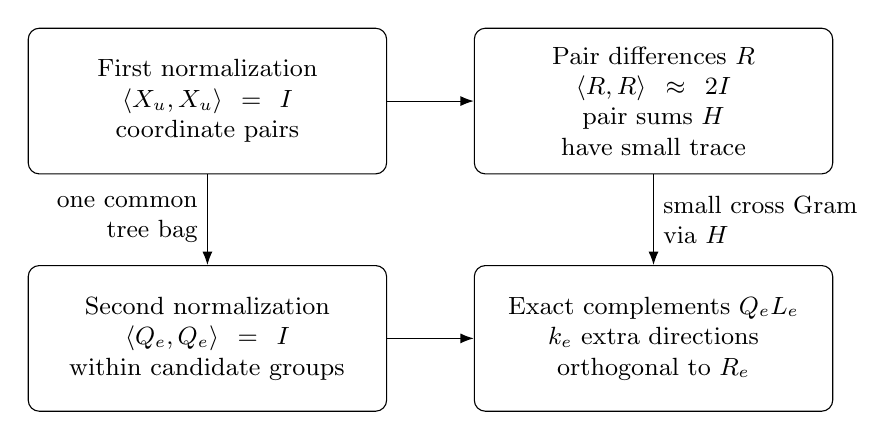
\begin{tikzpicture}[
  box/.style={draw,rounded corners,align=center,text width=4.2cm,
              minimum height=1.85cm,inner sep=5pt},
  >=Latex,font=\small]
\node[box] (first) {First normalization\\
  $\langle X_u,X_u\rangle=I$\\coordinate pairs};
\node[box,right=1.1cm of first] (sumdiff) {Pair differences $R$\\
  $\langle R,R\rangle\approx2I$\\pair sums $H$\\have small trace};
\node[box,below=1.15cm of first] (second) {Second normalization\\
  $\langle Q_e,Q_e\rangle=I$\\within candidate groups};
\node[box,right=1.1cm of second] (extra) {Exact complements $Q_eL_e$\\
  $k_e$ extra directions\\orthogonal to $R_e$};
\draw[->] (first)--(sumdiff);
\draw[->] (first)--node[left,align=right]{one common\\tree bag}(second);
\draw[->] (second)--(extra);
\draw[->] (sumdiff)--node[right,align=left]{small cross Gram\\via $H$}(extra);
\end{tikzpicture}
\caption{The two normalizations.  The common bag bounds all indicated
Gram matrices.  The trace estimate for $H$, followed by a spectral cutoff
at $2$, controls the interaction with the second normalization using an
absolute constant.}
\label{mr:two-scales}
\end{figure}

\subsection{The additional positive directions}

For each surviving pair $j=\{i,i'\}$ choose an order of its endpoints
and form
\[
 R_j=\frac{X_i-X_{i'}}{\sqrt2},
 \qquad H_j=\frac{X_i+X_{i'}}{\sqrt2}.
\]
The coefficient maps producing either list from $X$ are Euclidean
isometries.  The restriction of $I-W_s$ to retained pair endpoints has
Gram $2I$ on the difference coefficients.  Hence
\eqref{mr:matching-error} and contraction of Frobenius norm give
\begin{equation}\label{mr:R-bound}
 \|\langle R,R\rangle-2I_p\|_{\mathrm F}^2\le8\tau^2v.
\end{equation}
Also $\langle H_j,H_j\rangle=1-(B_s)_{ii'}$, so
\begin{equation}\label{mr:H-trace}
 |\Tr\langle H,H\rangle|\le p\tau\le\frac{\tau v}{2}.
\end{equation}
These statements persist after all the pair deletions: they are
restrictions of the original matching estimates.

The coefficients in each $D_e^{-1/2}$ are entrywise nonnegative.
Distinct groups have disjoint endpoint coordinates, and all cross Gram
entries between such coordinates are nonpositive.  Coordinates with
the same base label have zero interaction, since the first diagonal
blocks are identities.  Therefore
\begin{equation}\label{mr:Q-sign}
 \langle Q,Q\rangle=I-C_s,
 \qquad C_s\ge0\ \text{entrywise},
 \qquad (C_s)_{ee}=0\ \text{as a whole group block}.
\end{equation}
It is bounded in operator norm and has at most one negative eigenvalue.
By \Cref{mr:spectral-support}, its limiting spectral support lies in
$[0,2]$: more precisely, for every fixed $\varepsilon>0$ there are
$o(v)$ eigenvalues outside $[-\varepsilon,2+\varepsilon]$.
The joint Gram of $(H,Q)$ is bounded by the common bag.  Applying
\Cref{mr:trace-cross} to \eqref{mr:H-trace} yields the absolute estimate
\begin{equation}\label{mr:HQ-bound}
 \limsup_s\frac{\|\langle H,Q\rangle\|_{\mathrm F}^2}{v}
 \le\tau.
\end{equation}
In particular, no factor depending on the norm of the common bag
appears here.

Fix a candidate group $e\in\mathcal T$. Let $U_e$ be the
$2k_e\times k_e$ Euclidean isometry whose columns are the coefficient
vectors of its pair differences. Then
\[
 R_e=X_eU_e=Q_e T_e,
 \qquad T_e=D_e^{1/2}U_e.
\]
Because $D_e$ is positive definite, $T_e$ has rank exactly $k_e$.
Choose a $2k_e\times k_e$ matrix $L_e$ whose columns are an orthonormal
basis of $(\im T_e)^\perp$.  Thus
\begin{equation}\label{mr:exact-complement}
 L_e^{\mathsf T}L_e=I_{k_e},
 \qquad\langle R_e,Q_eL_e\rangle=T_e^{\mathsf T}L_e=0.
\end{equation}
This uses the full span of all the group's original difference
directions; no small singular direction is discarded.  Write
$L=\diag(L_e)_{e\in\mathcal T}$ and $Y=QL$.  The list $Y$ has
exactly $t$ columns.

For a pair $j$ outside group $e$, each of the two numbers
$x=\langle X_i,(Q_e)_k\rangle$ and
$y=\langle X_{i'},(Q_e)_k\rangle$ is nonpositive.  Consequently
\begin{equation}\label{mr:sign-domination}
 |\langle R_j,(Q_e)_k\rangle|
    =\frac{|x-y|}{\sqrt2}
    \le-\frac{x+y}{\sqrt2}
    =-\langle H_j,(Q_e)_k\rangle.
\end{equation}
This includes pairs in noncandidate groups.  Let $Z$ be
$\langle R,Q\rangle$ with the entries between each $R_e$ and its
own $Q_e$ replaced by zero.  Then
$\|Z\|_{\mathrm F}^2\le\|\langle H,Q\rangle\|_{\mathrm F}^2$,
and \eqref{mr:exact-complement} gives
$\langle R,Y\rangle=ZL$.  Since $L$ is an isometry, Frobenius
contraction and \eqref{mr:HQ-bound} imply
\begin{equation}\label{mr:RY-bound}
 \limsup_s\frac{\|\langle R,Y\rangle\|_{\mathrm F}^2}{v}
 \le\tau.
\end{equation}

Put $E_s=\langle Y,Y\rangle=L^{\mathsf T}\langle Q,Q\rangle L$.
Every diagonal group block of $E_s$ is an identity, so
\begin{equation}\label{mr:Y-trace}
 \Tr E_s=t.
\end{equation}
This is a Euclidean coefficient compression.  The variational
characterization of eigenvalues shows that the number of eigenvalues
of $E_s$ above $2+\varepsilon$ is at most that for
$\langle Q,Q\rangle$, hence is $o(v)$.  Its norm is bounded.
If $k_s$ denotes its number of eigenvalues greater than $1/4$, use
the cutoff $2+\varepsilon=5/2$ to obtain
\[
 t=\Tr E_s\le\frac{t-k_s}{4}+\frac52k_s+o(v).
\]
Possible negative eigenvalues only decrease the left-hand trace
contribution in this upper estimate.  Rearranging gives
\begin{equation}\label{mr:Y-positive-count}
 k_s\ge t/3-o(v).
\end{equation}

Finally consider the joint Gram matrix of $(R,Y)$.  By
\eqref{mr:R-bound}, the number of eigenvalues of
$\langle R,R\rangle$ at most $1/4$ is at most
\[
 \frac{16}{49}\|\langle R,R\rangle-2I_p\|_{\mathrm F}^2
 \le\frac{128}{49}\tau^2v.
\]
Restrict the two diagonal blocks to their spectral spaces above
$1/4$.  This leaves at least
$p-(128/49)\tau^2v$ dimensions on the $R$ side and
$t/3-o(v)$ on the $Y$ side.  The restricted cross matrix has squared
Frobenius norm at most $\|\langle R,Y\rangle\|_{\mathrm F}^2$.
Delete from the first side its left singular directions with singular
values greater than $1/8$.  The number deleted is at most
$64\|\langle R,Y\rangle\|_{\mathrm F}^2$.  The remaining diagonal
blocks are greater than $I/4$, and the cross operator norm is at most
$1/8$.  For their coefficient vectors $x,y$, the joint quadratic form
is bounded below by
\[
 \frac14(\|x\|^2+\|y\|^2)-\frac14\|x\|\|y\|
 \ge\frac18(\|x\|^2+\|y\|^2),
\]
so this remaining space is positive definite.  Using
\eqref{mr:RY-bound}, the positive index of the joint Gram is at least
\begin{equation}\label{mr:rank-gain}
 p+\frac t3-\frac{128}{49}\tau^2v-64\tau v-o(v).
\end{equation}
Every column used here is a linear combination of the original Lorentz
Gram columns for $M_s$.  The joint Gram is therefore a coefficient
pullback of $M_s$, and its positive index is at most $\rank M_s$.
This argument does not require the combined list $(R,Y)$ to be
linearly independent.

Combine \eqref{mr:final-pair-count}, \eqref{mr:extra-pair-count} and
\eqref{mr:rank-gain}.  Since $\tau\le1/8$,
\begin{align*}
 \liminf_s\frac{\rank M_s}{v}
 &\ge\frac12+\frac c9-64\tau-\frac{275}{49}\tau^2\\
 &\ge\frac12+\frac c9-65\tau
 \ge\frac12+\frac c{12},
\end{align*}
where the last inequality uses $\tau\le c/2340$.
This contradicts \eqref{mr:contradiction-rank}, whose normalized
right-hand side tends to $1/2$.  Hence only finitely many $s$ can
violate the stated rank bound.  The positive gap also shows directly
why the literal additive $+1$ is harmless for all sufficiently large
$s$.

Every matrix in the definition of $\mu(G[K_s])$ is among the matrices
just considered.  Rank--nullity gives
$\dim\ker M<ms/2-1$, and taking the maximum yields
$\mu(G[K_s])+1<ms/2$ as asserted.
\end{proof}

For completeness, the matrix class defining $\mu(H)$ is nonempty for
every finite nonempty graph $H$.  Start from a diagonal matrix with one diagonal
entry $-1$ and all others $1$, and put the same sufficiently small
negative number in each edge position.  The perturbation has operator
norm less than $1/2$ when its size is sufficiently small, so the matrix
is nonsingular with exactly one negative eigenvalue.  Nonsingularity
makes the Strong Arnold Property immediate.

If the base graph additionally satisfies $\alpha(G)\le2$, then
$\alpha(G[K_s])\le2$: an independent set uses at most one vertex of
each clique, and its base labels are independent.  Thus
$\chi(G[K_s])\ge\lceil ms/2\rceil>\mu(G[K_s])+1$.  Together with
\Cref{thm:base-graphs}, the theorem above proves \Cref{thm:main}.
One may also recover the chromatic number exactly as
$\chi(G[K_s])=ms-\nu(\overline{G[K_s]})$, where $\nu$ is the maximum
matching size: every color class has one or two vertices, and the
two-vertex classes are precisely disjoint hole pairs.

\section{The tensor geometry and the hole relation}\label{sec:geometry}

We construct a triangle-free relation of holes from tensor equations.
The complement of this relation will be our base graph; the moment
arguments in the next sections force its conflict properties.
All vector spaces, linear maps, tensor products and ranks in the construction are over \(\F=\mathbb F_2\).
We use the entrywise pairing of matrices:
\[
 \pair{A}{B}=\sum_{r,c}A_{rc}B_{rc}=\Tr(A\trans B).
\]
Probabilities and entropy take real values.

\subsection{The order of parameters}

We first fix the parameter hierarchy, then define the coefficient
space, its tensor-valued frame embeddings, and the hole equations.
The fixed constants below bound the information retained about a unit
and the number of vectors whose equality will certify a conflict.
Their order ensures that the colour-class scale precedes the graph
threshold, and that the thinning rate precedes the ambient dimension
multiplier.

The construction has one asymptotic parameter \(n\).  Every numerical parameter below, including the dimension multiplier \(M_0\), is fixed before \(n\) tends to infinity.
Set
\begin{equation}\label{eq:early-constants}
 C_0=1000,\qquad g=10^9+1,\qquad
 D=4C_0g,\qquad M=2^{1000},\qquad
 k_{\max}=56(g-1).
\end{equation}
In particular, \(g\) is odd.  The first pin budget and the entropy slack are
\begin{equation}\label{eq:pin-budgets}
 \zeta=\frac{1}{1000k_{\max}},
 \qquad K_1=\left\lceil\frac{4(D+1)}{\zeta}\right\rceil.
\end{equation}
For the phase estimates and a common upper bound on all pin dimensions, define
\begin{equation}\label{eq:law-budgets}
 \begin{gathered}
 r=2K_1+2,\qquad L_0=\lceil100(D+10)\rceil,\qquad
 d_0=4rL_0,\\
 u_0=10(K_1+d_0+1),\qquad
 K=\left\lceil\frac{10(D+K_1+u_0+10)}{\zeta}\right\rceil .
 \end{gathered}
\end{equation}
The budget \(K\) is a conservative upper bound; the construction uses only
the first peeling, whose pin dimension is at most \(K_1\).
The additional probability thresholds in \Cref{sec:phases} use only these early parameters and fixed numerical tolerances.  They do not depend on the selector or channel dimensions.

The early probability margins determine a colour cap \(\eta_{\rm col}>0\)
and then the graph class scale \(a>0\).  Given the graph threshold
\(\beta>0\), choose the endpoint-density bound \(L\) required in
\Cref{sec:graph-transfer}.  Next choose the selector parameters
\(j_*,b\) and the mixer parameters through \(J\) as in
\Cref{sec:moments}.  Choose \(r_0\) sufficiently large after those choices
and all fixed density bounds, and put \(h=1000r_0\).  After \(h\), choose
a sufficiently small thinning rate \(\rho>0\) as in
\Cref{sec:distributions}.  Finally choose a sufficiently large integer
\(M_0\), also relative to \(1/\rho\), and set
\begin{equation}\label{eq:parameter-order}
 \begin{gathered}
 (C_0,g,D,M,k_{\max},\zeta,K_1;\ r,L_0,d_0,u_0,K)\\
 \longrightarrow\ (\eta_{\rm col},a)
 \ \longrightarrow\ (\beta,L)
 \ \longrightarrow\ (j_*,b,\text{mixer parameters},J)\\
 \longrightarrow\ (r_0,h=1000r_0)
 \ \longrightarrow\ \rho
 \ \longrightarrow\ M_0,\qquad
 N=M_0n,\qquad m=2^{C_0gN}.
 \end{gathered}
\end{equation}
We always take \(n\ge 2r_0\) and subsequently increase its lower bound as needed.
The matrices used below have dimensions depending on \(n\); for each \(n\) they are chosen to satisfy \Cref{lem:generic-mixers}, before any law of units is considered.
The complete ledger of inequalities is in \Cref{sec:parameters}.

An \(O(n)\) bit count below has a constant depending only on parameters chosen before \(M_0\).
It can therefore be made a prescribed small fraction of \(N\).
This is different from an \(o(N)\) bound: after \(M_0\) is fixed, \(n/N=1/M_0\) is constant.
Later fixed tests and tolerances may change how large \(n\) must be; they do not change any earlier construction parameter.

\subsection{Moment matrices and cut profiles}

Let
\[
 \cI=\mathbb Z/g\mathbb Z,\qquad
 \cE=\binom{\cI}{2},\qquad
 I_d=\{d+1,\ldots,d+(g-1)/2\}\subset\cI .
\]
Elements of \(\cI\) are \emph{tags}; elements of \(\cE\) are \emph{components}.
The ordinary, or base, variables comprise \(g^2+3\) blocks of \(n\) bits:
\[
 O_{d,t}\quad(d,t\in\cI),\qquad S,\quad \#,\quad Z.
\]
A separate selector has \(b\) bits.  Its values \(s\in\F^b\) are called \emph{labels}, to distinguish them from tags.

The \(O\)-blocks carry testers whose availability depends on the tag,
while \(S\) carries a tester available at every tag.
The additional \(\#\)-block lets the self-Gram form \(E\), defined
below, distinguish different selector labels.
The \(Z\)-block is absent from \(E\); its free coordinates and
change-of-basis symmetry are used in the later parameter tests.

Let
\[
 p_*=\sum_{j=0}^{j_*}\binom bj,\qquad
 \cB=\F^{p_*}\otimes\F^{\,1+(g^2+3)n}.
\]
The first factor is indexed by squarefree selector monomials of degree at most \(j_*\); the second by the constant and the individual base variables.
If \(p_s\) is the vector of selector-monomial evaluations and \(z\) is a base value, write
\begin{equation}\label{eq:point-evaluation}
 v(s,z)=p_s\otimes(1,z)\in\cB.
\end{equation}
Thus the row and column coordinates both represent monomials of base degree at most one and selector degree at most \(j_*\).

Let \(W\subset\cB\otimes\cB\) be the span of the point moments \(v(s,z)v(s,z)\trans\).
For \(l\in\cI\), let \(W_l\) be the span of those point moments for which
\[
 O_{d,t}=0\quad\text{whenever }l\notin I_d.
\]
Let \(W_*\) be defined by requiring every \(O\)-block to be zero.
The cut-profile space is
\begin{equation}\label{eq:cut-profile-space}
 \cX=
 \left\{x=(x_{\{l,l'\}})_{\{l,l'\}\in\cE}:
 x_{\{l,l'\}}=w_l+w_{l'},\quad w_l\in W_l\right\}.
\end{equation}
A tuple \(w=(w_l)_{l\in\cI}\) as in this display is a \emph{representation} of \(x\).

\begin{lemma}\label{lem:cut-kernel}
The intersection of \(W_l\) over any strict majority of tags is \(W_*\).
Two representations of the same cut profile differ by a constant tuple with value in \(W_*\).
\end{lemma}
\begin{proof}
Fix a base coordinate in \(O_{d,t}\).  It is allowed at exactly \((g-1)/2\) tags.
A strict majority therefore contains a tag where that coordinate is disallowed.
Every row and column involving it is zero in \(W_l\) for that tag.
A matrix in the intersection consequently has zero rows and columns at all \(O\)-coordinates.

The coordinate projection that sets all \(O\)-variables to zero sends each point moment to a point moment defining \(W_*\).
Applied on both matrix factors, it fixes the matrix just described.
That matrix is therefore in \(W_*\), proving the nontrivial inclusion.

If \(w,w'\) give the same differences, then
\(w_l+w'_l=w_{l'}+w'_{l'}\) for every pair of tags.
Their difference is a constant tuple.  Its value belongs to every \(W_l\), hence to \(W_*\).
Conversely every such constant tuple lies in the kernel of the cut map.
\end{proof}

In each \(O_{d,t}\)-block and in \(S\), choose the first \(2r_0\) coordinates in disjoint ordered pairs.
The corresponding linear functionals on moments are
\[
 \eta_{d,t}\bigl(v(s,z)v(s,z)\trans\bigr)
   =\sum_{\rho=1}^{r_0}z_{O_{d,t},2\rho-1}z_{O_{d,t},2\rho},
 \qquad
 \eta_S\bigl(v(s,z)v(s,z)\trans\bigr)
   =\sum_{\rho=1}^{r_0}z_{S,2\rho-1}z_{S,2\rho}.
\]
They are well defined by selecting the indicated ordered matrix entries.
Put
\[
 \eta_O=\sum_{d,t}\eta_{d,t},\qquad \eta=\eta_O+\eta_S.
\]
For a cut profile represented by \(w\), define
\begin{equation}\label{eq:cut-functionals}
 \begin{aligned}
 a_t(x)&=\sum_{l,d}\eta_{d,t}(w_l),&
 a(x)&=\sum_t a_t(x)=\sum_l\eta_O(w_l),\\
 b_t(x)&=\sum_{l\ne t}\eta_S(w_l),&
 \chi_*(w)&=\sum_l\eta(w_l).
 \end{aligned}
\end{equation}
The functions \(a_t,a,b_t\) are well defined on \(\cX\).
Indeed, a constant kernel value in \(W_*\) contributes zero to every \(O\)-tester, while it contributes
\((g-1)\eta_S(w_*)=0\) to \(b_t\).
The quantity \(\chi_*(w)\) is used only when a representation has been specified.

Define a symmetric bilinear form \(T^0\) on \(\cX\) by
\begin{equation}\label{eq:T-zero}
 T^0=a\otimes a+\sum_{t\in\cI}(a_t\otimes b_t+b_t\otimes a_t).
\end{equation}
For \(1\le j\le J\) and ordered components \(e,f\), choose endomorphisms \(L_j^{ef},R_j^{ef}\) of \(\cB\).
Their required properties will be proved in \Cref{lem:generic-mixers}.
Set
\begin{equation}\label{eq:T-one}
 \begin{split}
 B^1(x,y)&=\sum_{j=1}^J\sum_{e,f\in\cE}
   \pair{x_e}{L_j^{ef}y_f(R_j^{ef})\trans},\\
 T^1(x,y)&=B^1(x,y)+B^1(y,x),\qquad
 T=T^0+T^1,\qquad
 r(x)=a+T(x,\cdot)\in\cX^*.
 \end{split}
\end{equation}
Here and later the letter \(r\) in \(r(x)\) denotes an affine-gradient map; the early integer \(r\) in \Cref{eq:law-budgets} is its separately specified rank budget.
Since the mixed terms in \(T^0(x,x)\) cancel, \(T^1\) is alternating, and \(a(x)^2=a(x)\), we have
\begin{equation}\label{eq:T-diagonal}
 T(x,x)=a(x)\qquad(x\in\cX).
\end{equation}

The prescribed self-frame Gram matrix is denoted by \(E\).
It is the sum of the ordered tester matrices for \(\eta\) and a matrix \(E^\#\) characterized on evaluation vectors by
\begin{equation}\label{eq:E-sharp}
 v(s,z)\trans E^\#v(s',z')
   =\sum_{\rho=1}^b(s_\rho+s'_\rho)\,z_\#\trans M_\rho z'_\# ,
\end{equation}
where \(M_\rho\) are \(n\)-by-\(n\) matrices chosen in \Cref{lem:generic-mixers}.
The expression is a bilinear form on \(\cB\) because \(j_*\ge1\).
It vanishes when the two point inputs coincide.
Consequently
\begin{equation}\label{eq:E-moments}
 \pair{E}{w}=\eta(w)\qquad(w\in W).
\end{equation}
The \(Z\)-block does not occur in \(E\).
In particular, any invertible linear change of the \(Z\)-variables preserves \(E\); this symmetry will be used in unary probability estimates.

\subsection{Raw vertices}

For each \(e\in\cE\), take copies \(V_e^+,V_e^-\) of \(\F^N\), paired by the usual dot product.
We regard \(V_e^-\) as the dual of \(V_e^+\) through that pairing.
A raw vertex, also called an \emph{orientation}, consists at each component of four maps
\[
 P_e,Q_e:\cB\longrightarrow V_e^+,V_e^-,
 \qquad X_e,Y_e:\F^h\longrightarrow V_e^+,V_e^-,
\]
where the target is the first or second one as appropriate.
They satisfy
\begin{equation}\label{eq:raw-frame-law}
 [P_e,X_e]\text{ and }[Q_e,Y_e]\text{ are injective},\qquad
 P_e\trans Q_e=E,\quad X_e\trans Q_e=0,\quad P_e\trans Y_e=0.
\end{equation}
No value is prescribed for \(X_e\trans Y_e\).

Write \(d=\dim\cB\).
For all large \(n\), \(N\ge2(d+h)\), by the final choice of \(M_0\).
The frame set is then nonempty.
For example, take the plus columns to be the first \(d+h\) coordinate vectors.
Prescribe the full \((d+h)\)-square Gram matrix to be
\(\begin{psmallmatrix}E&0\\0&0\end{psmallmatrix}\).
Lift its columns to minus vectors using the first \(d+h\) coordinates, and append distinct coordinate vectors in a complementary space of dimension \(d+h\).
These minus columns are independent and have the desired Gram values.

Take the uniform distribution on this finite frame set, independently over components.
Let \(\Omega_n\) be the raw vertex space and \(\rawlaw=\rawlaw_n\) this distribution.
We call \(P_e,Q_e\) the primal maps and \(X_e,Y_e\) the channel maps.
The sampling law \(\pi=\pi_n\), defined in \Cref{sec:distributions},
will preserve the \(\rawlaw\)-marginal of all primal maps and restrict
the conditional channel choices.  All identities in this section hold
for every raw vertex, and therefore under either law.
There are at most \(2^{2|\cE|N(d+h)}\) raw vertices, so
\begin{equation}\label{eq:raw-space-size}
 \log_2|\Omega_n|=O(N^2).
\end{equation}

Use the common ambient tensor space
\[
 \cV=\bigoplus_{e\in\cE}V_e^+\otimes V_e^-.
\]
For a raw vertex \(o\), define
\begin{equation}\label{eq:raw-embedding}
 U_o x=(P_{o,e}x_eQ_{o,e}\trans)_{e\in\cE},
 \qquad
 u_o(\xi)=\sum_{e\in\cE}\pair{Y_{o,e}X_{o,e}\trans}{\xi_e}.
\end{equation}
On a simple tensor \(pq\trans\) in component \(e\), the latter pairing is
\[
 u_o(pq\trans)=(Y_{o,e}\trans p)\cdot(X_{o,e}\trans q).
\]
Thus the minus channel is paired with the first tensor factor and the plus channel with the second.
All copies of coefficient spaces attached to different vertices are distinct, although the ambient \(V_e^\pm\) are common.

Each \(U_o\) is injective: a left inverse of \(P_{o,e}\) and the transpose of a left inverse of \(Q_{o,e}\) recover \(x_e\) from \(P_{o,e}x_eQ_{o,e}\trans\).
The two annihilator conditions in \Cref{eq:raw-frame-law} also give
\begin{equation}\label{eq:self-contraction-zero}
 u_oU_o=0.
\end{equation}

\begin{definition}\label{def:hole}
Two raw vertices \(i,j\) have a \emph{hole} between them if there exist \(\lambda_i,\lambda_j\in\cX\) such that
\begin{equation}\label{eq:hole-equations}
 \begin{gathered}
 U_i\lambda_i=U_j\lambda_j,\qquad
 u_jU_i=r(\lambda_i),\qquad u_iU_j=r(\lambda_j),\\
 a(\lambda_i)+a(\lambda_j)=1.
 \end{gathered}
\end{equation}
The middle two identities are identities of linear functionals on the whole cut-profile space.
\end{definition}

\begin{lemma}\label{lem:hole-triangle-free}
The hole relation is symmetric, has no loops, and is triangle-free.
\end{lemma}
\begin{proof}
Symmetry follows by interchanging the endpoints.
A loop would have \(U_i\lambda_i=U_i\lambda_j\), hence \(\lambda_i=\lambda_j\) by injectivity, contradicting the last equation of \Cref{eq:hole-equations}.

Suppose that three distinct raw vertices have holes on all three pairs.
For a directed incidence \(ij\), let \(x_{ij}\) be its witness at \(i\).
For distinct \(i,j,k\), evaluate the gradient identity for \(ij\) on \(x_{ik}\):
\[
 u_j(U_ix_{ik})=a(x_{ik})+T(x_{ij},x_{ik}).
\]
Sum over the six ordered choices of \((i,j,k)\).
For fixed \(j\), the two arguments on the left are equal by the sharing equation for the remaining edge \(ik\), so they cancel.
For fixed \(i\), the two bilinear terms cancel by symmetry of \(T\).
The remaining sum is
\[
 \sum_{\{i,j\}}\bigl(a(x_{ij})+a(x_{ji})\bigr)=1+1+1=1,
\]
a contradiction.
\end{proof}

Sample \(m\) raw vertices independently from the law \(\pi\) defined in
\Cref{sec:distributions}, and form \(G\) on their \emph{positions}: two distinct positions are adjacent when their raw types have no hole.
This gives a finite simple graph even when types repeat.
Equal raw types are adjacent because holes have no loops.
An independent triple of positions would therefore give three distinct raw types forming a hole triangle.
By \Cref{lem:hole-triangle-free},
\begin{equation}\label{eq:sample-independence}
 \alpha(G)\le2,\qquad \chi(G)\ge\lceil m/2\rceil.
\end{equation}

\section{The distribution problem and its preliminary tools}\label{sec:distributions}

A \emph{unit} is an ordered pair of raw vertices with no hole between its endpoints.
The endpoints of a unit may be dependent.
When two units are sampled independently, their four endpoints need not be independent within either unit.
The event of interest is that all four cross pairs have holes, as in \Cref{fig:four-holes}.

The raw reference law \(\rawlaw\) is the uniform law of the exact frames in
\Cref{eq:raw-frame-law}.  We will replace its conditional channel law by a
thinned law \(\pi\), while preserving its primal marginal exactly.
The reference image and peeling arguments below use the absolute joint cap
\begin{equation}\label{eq:raw-law-caps}
 \sigma\le 2^{DN}\rawlaw^2.
\end{equation}
This condition alone imposes no constant bound on either endpoint marginal.
The stronger marginal hypotheses required for the distribution tests will
always be stated separately, relative to \(\pi\).

\subsection{Uniform frame laws}

We record the linear algebra behind all reference image laws.
For a subspace of a nominal coefficient space, its \emph{image} is its image under the relevant frame map.
Nominal independence is independence before applying these maps.

\begin{lemma}\label{lem:paired-frame-orbit}
Let \(A,A':U\to V\) and \(B,B':W\to V^*\) be injective maps between finite-dimensional spaces over \(\F\).
If
\[
 B\trans A=(B')\trans A',
\]
there is \(L\in\GL(V)\) with \(LA=A'\) and \(L^{-\mathsf T}B=B'\).
Thus based individually injective plus and minus frames with a prescribed Gram matrix form one orbit under the simultaneous primal and dual action.
\end{lemma}
\begin{proof}
Write \(\Phi=B\trans:V\to W^*\) and \(\Phi'=(B')\trans:V\to W^*\).
Both are surjective.
The based map \(f:A(U)\to A'(U)\) given by \(f(Au)=A'u\) satisfies \(\Phi'f=\Phi\).
It therefore maps \(A(U)\cap\ker\Phi\) isomorphically onto \(A'(U)\cap\ker\Phi'\).
Extend this restriction to an isomorphism \(L_0:\ker\Phi\to\ker\Phi'\).

Choose a complement \(U_0\) of \(A(U)\cap\ker\Phi\) in \(A(U)\).
Its images under \(\Phi\) are independent.
Extend a basis of \(\Phi(U_0)\) to a basis of \(W^*\), and choose lifts of the added basis vectors under \(\Phi\) and \(\Phi'\), respectively.
For the basis vectors in \(\Phi(U_0)\), choose the lifts in \(U_0\) and their images under \(f\).
Define \(L\) to equal \(L_0\) on \(\ker\Phi\) and to carry each chosen lift to its primed lift.
These are direct-sum decompositions of \(V\), so \(L\) is an isomorphism.
It extends \(f\) and satisfies \(\Phi'L=\Phi\), which is equivalent to the two required frame identities.
\end{proof}

\begin{lemma}\label{lem:frame-images}
The following statements hold for all sufficiently large \(n\).
\begin{enumerate}[label=\textup{(\alph*)}]
\item
At independently sampled raw vertices and components, images of prescribed primal coefficient tuples that are independent separately at each vertex and sign are uniform subject to their individual injectivities and their prescribed same-vertex Gram matrices.
For tuples using channels as well, the same assertion holds conditionally on the full self-channel Gram matrices \(X_e\trans Y_e\); the relevant full Gram matrix is
\(\begin{psmallmatrix}E&0\\0&X_e\trans Y_e\end{psmallmatrix}\).

\item
Let a fixed tuple of nominal directions use arbitrary combinations of the two endpoints' primal and channel coefficients.
Compute its rank separately in each component and sign in the \emph{direct sum over both endpoints}, and let the total be \(t\).
For every preassigned \(\epsilon>0\), choosing \(M_0\) sufficiently large gives, under \(\rawlaw^2\),
\begin{equation}\label{eq:reference-image-cap}
 \PP\{\text{all those images equal prescribed vectors}\}
 \le 2^{-(1-\epsilon)tN}\qquad(t\ge1).
\end{equation}
This is valid for all possible ranks \(t\), including \(t=O(n)\), not only for bounded tuples.

\item
The plus frame \([P,X]\) is uniform among injective maps.
Conditional on it, the minus columns are independent uniforms on the affine spaces prescribed in \Cref{eq:raw-frame-law}, followed only by the conditioning that \([Q,Y]\) is injective.
The failure probability of this last condition, before conditioning, is at most \(2^{2(d+h)-N}\) per component.

Given \(P,Q\), the channels \(X,Y\) are independent uniform-column draws on \(\ker Q\trans\) and \(\ker P\trans\), respectively, conditioned on \([P,X]\) and \([Q,Y]\) being injective.
The two rank-failure probabilities are exponentially small in \(N\).
Each channel frame alone is uniform among injective maps \(\F^h\to\F^N\).
For any fixed \(q\) independent vectors in its paired ambient space, the probability that transpose evaluation on their span is not injective is at most
\begin{equation}\label{eq:channel-transpose-failure}
 2^{q-h+1}.
\end{equation}
The unconditional joint channel law is bounded above by a constant, depending on \(g,h\) but not on \(n\), times the completely independent uniform-column law.

\item
For \(p\) independent uniform plus vectors and \(q\) independent uniform minus vectors in paired copies of \(\F^N\), and a prescribed \(p\)-by-\(q\) Gram matrix \(G\), the probability of that Gram matrix together with individual injectivity of both frames is at most \(2^{-pq}\) and at least
\begin{equation}\label{eq:bounded-gram-normalization}
 2^{-pq}(1-2^{p-N})(1-2^{p+q-N}).
\end{equation}
In particular, any consistent Gram specification on a bounded number of vectors, together with injectivity on each side, has probability bounded below by a positive constant for large \(N\).
\end{enumerate}
\end{lemma}
\begin{proof}
The raw law is invariant under \(L\) on each \(V_e^+\) and \(L^{-\mathsf T}\) on \(V_e^-\), independently at vertices and components.
For primal tuples, their restricted Gram is fixed by \(E\).
By \Cref{lem:paired-frame-orbit}, all based realizations with that Gram and individual injectivity lie in one orbit.
Projection of an invariant uniform raw law is uniform on this orbit: an element carrying one partial realization to another bijects their full-frame completions.
There is at least one completion because these tuples are restrictions of a raw frame.
After fixing \(X_e\trans Y_e\), the same argument applies to arbitrary full-frame coefficient tuples.
Independence over raw draws and components proves (a).

For (c), the action is transitive on injective plus frames, so their marginal is uniform.
Given a plus frame, each column of \(Q\) has specified evaluations against \(P,X\), while each column of \(Y\) has zero evaluations against \(P\).
There is no other constraint until full minus injectivity is imposed.
The remaining allowed set is therefore the product of those affine column spaces restricted to full rank.

Each column space contains the common translation space
\(\operatorname{ann}(\im[P,X])\), of dimension \(N-d-h\).
For a nonzero coefficient vector \(c\in\F^{d+h}\), the corresponding linear combination of minus columns is consequently uniform on an affine space containing that translation space.
Its chance of being zero is at most \(2^{-(N-d-h)}\).
Union over the fewer than \(2^{d+h}\) nonzero coefficient vectors gives the asserted bound \(2^{2(d+h)-N}\).

Alternatively, condition first on \(P,Q\).
The allowed \(X\)-columns lie in \(\ker Q\trans\), the allowed \(Y\)-columns in \(\ker P\trans\), and their two full-rank restrictions are separate.
This proves the stated conditional independence.
For example, before imposing injectivity of \([P,X]\), any dependence with a nonzero \(X\)-coefficient has probability at most \(2^{-(N-d)}\); union over its at most \(2^{d+h}\) coefficient choices gives a bound \(2^{2d+h-N}\).
The estimate for \(Y\) is identical.

The marginal of \(X\) alone is invariant under \(\GL(\F^N)\) and supported on injective maps; transitivity gives its uniformity, and likewise for \(Y\).
Before conditioning independent channel columns to be injective, their evaluations on a fixed independent \(q\)-tuple form a uniform \(h\)-by-\(q\) matrix.
For each nonzero coefficient vector in \(\F^q\), the chance that its evaluation is zero is \(2^{-h}\).
Union over those coefficient vectors gives at most \(2^{q-h}\), and channel injectivity has probability at least \(1/2\) for large \(N\).
This proves \Cref{eq:channel-transpose-failure}.
To compare their joint marginal with completely independent columns, condition on \(G=X\trans Y\).
The conditional marginal is uniform on the orbit of two individually injective \(h\)-frames having Gram matrix \(G\).
Under independent uniform columns that orbit has probability at least \(2^{-h^2-2}\) for large \(N\), by the argument for (d) below.
Since the raw probability of any \(G\) is at most one, the density ratio on every such orbit is at most \(2^{h^2+2}\).
Multiply over the fixed number of components to obtain the joint channel bound.
Its possible dependence on \(h\) is harmless: \(h\) is fixed before \(n\) grows.

We next prove (b), keeping explicit the dependence on the rank.
Replace each tested tuple by a basis of its nominal span; inconsistent dependent prescriptions have probability zero.
For the plus directions at the two endpoints, start with completely independent uniform plus columns and then impose individual full-frame injectivity.
The image of a rank-\(t_+\) tuple in the joint nominal direct sum is exactly uniform on \(t_+\) independent ambient vectors before this conditioning.
Indeed, at each ambient coordinate the coefficient map is a surjective linear map onto \(\F^{t_+}\), and different ambient coordinates use independent input bits.
Full injectivity has probability \(1-2^{-\Omega(N)}\), uniformly over the given construction, so the plus prescription costs at most
\((1-2^{-\Omega(N)})^{-1}2^{-t_+N}\).

Now condition on all plus frames.
At a component let \(S\) be the span of both endpoints' plus columns; then \(\dim S\le2(d+h)\).
Before minus injectivity, every minus column has an affine distribution whose translation space contains \(S^\perp\).
Split off an independent uniform \(S^\perp\)-part of each column and condition on the remaining parts.
For a rank-\(t_-\) tuple of minus coefficient combinations, the \(S^\perp\)-parts of its images are independent uniform vectors in \(S^\perp\), because the coefficient map has rank \(t_-\).
Thus prescribed minus images have probability at most
\[
 2^{-(N-2(d+h))t_-}.
\]
The additional conditioning on the two minus frames being injective changes this by a factor \(1+2^{-\Omega(N)}\), by (c).
Perform this argument componentwise.
There is a fixed total conditioning factor bounded, for example, by \(4^{|\cE|}\), and the resulting bound is
\[
 4^{|\cE|}\,2^{-t_+N-(N-2(d+h))t_-}.
\]
Choose \(M_0\) so that \(2(d+h)/N<\epsilon/2\) for large \(n\), and then increase \(n\) so that the fixed prefactor is at most \(2^{\epsilon N/2}\).
Since \(t=t_++t_-\ge1\), this proves \Cref{eq:reference-image-cap} uniformly for every allowable \(t\).
In particular, mixing the two endpoints in a direction causes no loss of an entire \(N\)-bit image constraint.

Finally, to prove (d), the plus columns are independent with probability at least \(1-2^{p-N}\): each nonzero coefficient dependence has probability \(2^{-N}\).
Given their independence, each minus column takes its required evaluations with probability \(2^{-p}\), independently, so the Gram costs \(2^{-pq}\).
Under this Gram conditioning, every nonzero combination of minus columns is uniform on an affine space of dimension at least \(N-p\).
Its probability of vanishing is at most \(2^{-(N-p)}\).
Union over fewer than \(2^q\) combinations gives failure probability at most \(2^{p+q-N}\).
This proves the lower bound.
For the upper bound with plus injectivity required, condition on the plus columns and use the exact \(2^{-pq}\) Gram probability whenever they are independent.
A partially specified consistent Gram contains some full specification; for bounded \(p,q\), the same positive lower bound for that full specification proves the last assertion.
\end{proof}

\subsection{Thinning the channel images}

Write \(e_* = |\cE|\), \(d=\dim\cB\), and
\[
 q_h=2^h-1,\qquad k_h=2e_*q_h,\qquad
 \varepsilon_{\rm ch}=10e_*2^h\rho.
\]
After the channel dimension \(h\) has been fixed, choose \(\rho>0\) so small
that \(10^4e_*2^{2h}\rho<\zeta/100\) and that this quantity is smaller than
every fixed rate slack used below.  We then choose \(M_0\) large enough
also in terms of \(1/\rho\).  The channel frame in sign \(+\) is \(X_e\),
and that in sign \(-\) is \(Y_e\).

\begin{lemma}[Channel thinning]\label{lem:channel-thinning}
Fix any bound \(q_{\rm test}\) on the lengths of the ambient tuples to be tested;
this bound is fixed before \(\rho,M_0,n\).  For all sufficiently large \(n\)
there are subsets \(A_e^\pm\subseteq V_e^\pm\), each of density
\((1+o(1))2^{-\rho N}\), with the following properties.
Keep the \(\rawlaw\)-marginal on all primal frames \((P_e,Q_e)_e\).
Given those frames, condition the original channel law on
\begin{equation}\label{eq:channel-allowed}
 X_e c\in A_e^+,\qquad Y_e c\in A_e^-
 \quad(e\in\cE, 0\ne c\in\F^h).
\end{equation}
This conditional event has positive probability for every primal frame.
The resulting probability law \(\pi\) satisfies:
\begin{enumerate}[label=\textup{(\alph*)}]
\item Its primal marginal is exactly that of \(\rawlaw\), and
\begin{equation}\label{eq:thinning-density}
 \pi^2\le 2^{\varepsilon_{\rm ch}N}\rawlaw^2.
\end{equation}
\item For every fixed independent ambient \(q\)-tuple, \(q\le q_{\rm test}\),
transpose evaluation by any specified channel frame has failure probability
at most \(2^{q-h+1}+o(1)\) under \(\pi\), uniformly in the tuple.
More generally every fixed finite union of these rank-failure tests has its
\(\rawlaw\)-probability plus \(o(1)\) as an upper bound.
\item Given any primal frames, any component and sign, and any nonzero
\(v\in V_e^\pm\),
\begin{equation}\label{eq:channel-translate}
 \pi\bigl\{\exists c\ne0:\ X_ec\in A_e^++v
              \mid(P,Q)\bigr\}\le2^{-\rho N/2},
\end{equation}
with the analogous statement for \(Y_e,A_e^-\).
\end{enumerate}
The error in \textup{(b)} is exponentially small in \(N\).
The ambient tuple there is fixed before sampling the vertex; no uniform
conditional rank bound for a tuple selected from the sampled primal frame
is asserted.
\end{lemma}
\begin{proof}
Include every ambient vector in each \(A_e^\pm\) independently with
probability \(p=2^{-\rho N}\); subsets for different components and signs
are independent.  Fix a complete primal frame \(f\), and let \(\nu_f\)
be the original conditional channel law.  Define its survival fraction
\(Z_f=\nu_f(\text{\Cref{eq:channel-allowed}})\), a random variable in the
random subsets.  Channel injectivity makes the \(q_h\) nonzero values in
each component and sign distinct.  Consequently
\[
 \mathbb E_A Z_f=p^{k_h}.
\]
For any transpose-rank test \(T\), or any union of at most \(N\)
such tests, the numerator
\(Z_{f,T}=\nu_f(T\cap\text{\Cref{eq:channel-allowed}})\) similarly has
expectation \(p^{k_h}\nu_f(T)\).

We establish simultaneous concentration of these fractions by the
bounded-differences method \citep{azuma1967,mcdiarmid1989}, with the
needed exponential-moment estimate included below.  By
\Cref{lem:frame-images}(c), a prescribed nonzero channel combination,
conditional on \(f\), has probability at most \(2^{-(N-d)+1}\) of taking
any prescribed value for all sufficiently large \(N\).  Indeed before
full-frame injectivity it is uniform on the appropriate annihilator,
and injectivity has probability \(1-2^{-\Omega(N)}\), uniformly in \(f\).
Changing one membership bit of a subset can therefore change any such
fraction by at most
\[
 c_N=C_h2^{-N+d},
\]
where \(C_h\) is fixed in \(n\).  There are \(2e_*2^N\) membership bits,
so the sum of their squared influence bounds is at most
\[
 S_N=C_{g,h}2^{-N+2d}.
\]
For clarity, expose these independent bits and use the Doob martingale
of any one fraction.  A centered increment whose conditional range has
length at most \(c\) has exponential moment at most \(\exp(t^2c^2/8)\).
To see this, the second derivative of its log moment generating function
is the variance under an exponential tilt, at most \(c^2/4\); integrate
twice using value and derivative zero at the origin.  Multiplication of
the conditional bounds and Markov's inequality give
\[
 \Pr_A(|Z-\mathbb E_AZ|>u)\le2\exp(-2u^2/S_N).
\]
Take \(u=\epsilon_N=2^{-N/10}\).  Since \(d/N\) can be made arbitrarily
small by increasing \(M_0\), these tails are at most
\(2\exp(-c_{g,h}2^{N/2})\).  There are \(2^{O(N^2)}\) primal frames and \(2^{O(N)}\) primitive
transpose tests, since their tuple lengths are bounded by the fixed
\(q_{\rm test}\).  The unions of at most \(N\) primitive tests therefore
number at most \(2^{O(N^2)}\) as well.  A union bound gives simultaneous
error at most \(\epsilon_N\) for all these denominators and test numerators.
The same argument for \(2^{-N}|A_e^\pm|\), whose bit influences are
\(2^{-N}\), gives \(|A_e^\pm|/2^N=(1+o(1))p\).

We include the translated numerators in this simultaneous estimate.
Fix \(f,e,\pm,v\ne0\), and let \(Z_{f,v}^{\pm,e}\) be the original
conditional probability of survival and of the event in
\Cref{eq:channel-translate}.  Consider, for example, sign \(+\).
If \(X_ec+v\) coincides with another already required nonzero channel
value \(X_ec'\), then \(v=X_e(c+c')\) is a nonzero channel value.
The original probability of this possibility is at most
\(C_h2^{-N+d}\), by the point bound and a union over the nonzero
coefficients.  On that exceptional event we bound the extra test by one;
the survival probability over the random subsets is still \(p^{k_h}\).
In every other case \(X_ec+v\) is a new membership bit and supplies an
additional factor \(p\).  This includes the case \(X_ec+v=0\), since
zero is not among the required nonzero channel values.  Union over \(c\)
yields
\[
 \mathbb E_AZ_{f,v}^{+,e}
 \le p^{k_h}\bigl(C_h2^{-N+d}+q_hp\bigr).
\]
A changed membership bit can affect this numerator only by being an
original channel value or a translated channel value.  Both have point
probability at most \(C_h2^{-N+d}\); hence the same influence and
concentration estimates apply.  The additional \(2^N\) choices of
translate do not affect the union bound.  We may therefore fix one
realization of all subsets for which every displayed concentration
statement holds simultaneously.

Our choice of \(\rho\) gives \(k_h\rho<1/100\).  Thus
\[
 Z_f=p^{k_h}(1+O(\epsilon_N/p^{k_h}))>0
\]
uniformly, and the relative error tends to zero exponentially.
The pointwise density of \(\pi\) with respect to \(\rawlaw\) is the
survival indicator divided by \(Z_f\).  Consequently
\[
 \frac{d\pi^2}{d\rawlaw^2}
 \le4p^{-2k_h}\le2^{\varepsilon_{\rm ch}N}
\]
for large \(N\); the primal law was left unchanged by definition.
Division of \(Z_{f,T}\) by \(Z_f\) gives
\(\pi(T\mid f)=\nu_f(T)+O(\epsilon_N/p^{k_h})\), uniformly in every
specified fixed test.  Average over the original primal marginal and
apply \Cref{eq:channel-transpose-failure} to prove \textup{(b)}.  Every
fixed finite union is among our tested unions once \(N\) is large enough;
applying the same numerator estimate directly to that union gives its
raw probability plus the stated error, without replacing the union
probability by the sum of its constituent probabilities.  Finally,
dividing the translated
numerator by \(Z_f\) bounds it by
\[
 C_h2^{-N+d}+q_h2^{-\rho N}
       +O(\epsilon_N/p^{k_h})\le2^{-\rho N/2}
\]
for all sufficiently large \(N\).  This proves \textup{(c)} and the lemma.
\end{proof}

\subsection{The two distribution tests}

For independent units \(A=(A_1,A_2)\), \(B=(B_1,B_2)\), write
\(A\bowtie B\) when all four pairs \((A_i,B_j)\) are holes.  For a point
\(z\), write \(A\bowtie z\) when both \((A_i,z)\) are holes.
These definitions also cover repeated raw types; the absence of hole
loops automatically forbids a conflict with a shared endpoint.

\begin{theorem}[Distribution tests]\label{thm:distribution-tests}
There is a constant \(\eta_{\rm col}>0\), depending only on the early
parameters and \(M\), with the following property.  Fix any \(L<\infty\)
after \(\eta_{\rm col}\) and before the selector and channel parameters;
choose all remaining parameters in the order of
\Cref{eq:parameter-order,sec:parameters}.  For every sufficiently large
\(n\), the law \(\pi\) constructed above satisfies both conclusions.
\begin{enumerate}[label=\textup{(\roman*)}]
\item Let \((A,c)\) have a probability law on units marked by a colour in
any fixed finite palette.  The colour may be randomized conditional on
\(A\).  Write \(\sigma_1,\sigma_2\) for the endpoint
marginals of its projected unit law \(\sigma\), and suppose
\begin{equation}\label{eq:coloured-law-caps}
 \sigma_1\le M\pi,\qquad \sigma_2\le M\pi,\qquad
 \sigma\le2^{3000gN}\pi^2,
 \qquad \Pr(c=j)\le\eta_{\rm col}\quad\text{for every }j.
\end{equation}
For two independent draws \((A,c),(B,c')\),
\[
 \Pr(A\bowtie B, c\ne c')\ge2^{-100gN}.
\]
\item Let \(A\) have a unit law \(\sigma\) and let \(z\) be an independent
point with law \(\theta\), where
\begin{equation}\label{eq:asymmetric-law-caps}
 \sigma_1\le L\pi,\qquad \sigma_2\le L\pi,\qquad
 \sigma\le2^{3000gN}\pi^2,
 \qquad \theta\le L\pi.
\end{equation}
Then \(\Pr(A\bowtie z)\ge2^{-100gN}\).
\end{enumerate}
The threshold for \(n\) may depend on the fixed palette and on \(L\).
All inequalities between measures are pointwise on their finite spaces.
\end{theorem}

The two conclusions are proved after the collision and overlap arguments,
in \Cref{prop:coloured-distribution,sec:asymmetric-test}, respectively.
The finite graph transfer is given in \Cref{sec:graph-transfer}.
Here we establish their leaf and image hypotheses.  In particular,
\Cref{eq:thinning-density} places every projected test law below
\(2^{(3000g+\varepsilon_{\rm ch})N}\rawlaw^2\), leaving strict slack
below the absolute budget \(D=4000g\).

\subsection{Sparse profiles arising from true intersections}

For a matrix profile, its \emph{total component rank} means \(\sum_{e\in\cE}\rank x_e\).

\begin{lemma}\label{lem:raw-intersections}
Let \(\sigma\) satisfy the joint cap in \Cref{eq:raw-law-caps}.
Outside a set of \(\sigma\)-probability \(2^{-\Omega(N)}\),
\[
 \sum_{e\in\cE}
  \dim\bigl(\im P_{1,e}\cap\im P_{2,e}\bigr)\le2D.
\]
For any unit outside that exceptional set and any
\(U_1\lambda_1=U_2\lambda_2\), both \(\lambda_i\) have total component rank at most \(2D\).
Each has a unique representation \((w_{i,l})_l\) vanishing at a strict majority of tags, and
\[
 |\{l:w_{i,l}\ne0\}|\le4D/g,\qquad
 \chi_*(w_1)=\chi_*(w_2).
\]
\end{lemma}
\begin{proof}
If the summed intersection dimension exceeds \(2D\), choose \(2D\) independent common-image vectors, componentwise.
Write each as \(P_{1,e}a=P_{2,e}b\).
Their nominal relation directions \((a,b)\) are independent in the direct sum of the two primal coefficient spaces at that component.
Indeed a dependence between the pairs would, after applying \(P_{1,e}\), be the corresponding dependence between the selected common-image vectors.
Across components their ranks add.

There are at most \(2^{O(n)}\) ways to choose this bounded number of coefficient pairs and their component indices.
For each choice, \Cref{eq:reference-image-cap} bounds the probability of their zero images by \(2^{-(1-\epsilon)2DN}\) under \(\rawlaw^2\).
After paying \(2^{DN}\) for \(\sigma\), and making the coefficient count a sufficiently small fraction of \(N\) by the choice of \(M_0\), the union bound is \(2^{-\Omega(N)}\).

Suppose \(U_1\lambda_1=U_2\lambda_2=\xi\).
The column space of \(\xi_e\) lies in both primal plus spans.
Since multiplication by the two injective frame maps preserves matrix rank,
\[
 \rank(\lambda_{i,e})=\rank(\xi_e)
 \le\dim(\im P_{1,e}\cap\im P_{2,e}).
\]
This proves the total-rank assertion.

Take any representation \((w_l)_l\) of one of the profiles.
A component \(w_l+w_{l'}\) is nonzero whenever \(w_l\ne w_{l'}\), so there are at most \(2D\) unequal unordered pairs.
If no value occurred at a strict majority of tags, write \(c_v\) for its multiplicities.
Then
\[
 \#\{\text{unequal pairs}\}
 =\frac12\left(g^2-\sum_vc_v^2\right)
 \ge\frac12\left(g^2-\frac g2\sum_vc_v\right)
 =\frac{g^2}{4}>2D,
\]
a contradiction.
Let the majority have size \(g-z\).
There are at least \(z(g-z)\ge zg/2\) unequal pairs, hence \(z\le4D/g\).
Its common value belongs to \(W_*\) by \Cref{lem:cut-kernel}, so subtract it from every coordinate.
The resulting representation vanishes at a strict majority.
It is unique: two such representations differ by a constant, and their two majority zero sets intersect.

Finally, equality of the component tensors gives equality of their ambient traces.
By cyclicity of trace and \Cref{eq:E-moments},
\[
 \Tr(P_{i,e}\lambda_{i,e}Q_{i,e}\trans)
 =\pair{P_{i,e}\trans Q_{i,e}}{\lambda_{i,e}}
 =\eta(\lambda_{i,e}).
\]
For \(e=\{l,l'\}\), it follows that
\[
 \eta(w_{1,l})+\eta(w_{2,l})
 =\eta(w_{1,l'})+\eta(w_{2,l'}).
\]
This value is independent of the tag.
The two sparse representations together have at most \(8D/g=32000<g\) nonzero coordinates, so some tag has both entries zero.
The common value is therefore zero.
Summing over tags proves equality of the two specified \(\chi_*\)-values.
\end{proof}

\subsection{Peeling into leaves with exact pins}

For a unit \(O=(1,2)\), introduce nominal coefficient spaces at each component
\[
 \cL_{O,e}
   =\bigoplus_{i\in O}(\cB_i\oplus H_i^+),
 \qquad
 \cR_{O,e}
   =\bigoplus_{i\in O}(\cB_i\oplus H_i^-),
 \qquad H_i^\pm=\F^h.
\]
Their frame-image maps add the endpoint images in the common ambient \(V_e^\pm\).
A \emph{pin space} is a specified subspace \(D_{O,e}^\pm\) of this nominal direct sum together with specified exact images of every vector in a chosen basis.
It may mix both endpoints, and it may mix primal and channel coordinates.
Once the basis images are known, every image on the pin space is fixed.

For a tested tuple of directions, its \emph{rank modulo the pins} is the sum, over components and signs, of the dimensions of the spans of its images in the quotients by \(D_{O,e}^\pm\).
The rank is nominal; it is not computed after applying the raw frames.

\begin{lemma}[First peeling and restriction]\label{lem:peeling}
Take the constants in \Cref{eq:pin-budgets,eq:law-budgets}, and choose the reference accuracy in \Cref{eq:reference-image-cap} with \(\epsilon<\zeta/4\).
For every law \(\sigma\) satisfying the absolute joint cap \Cref{eq:raw-law-caps}, the following decompositions are available.
\begin{enumerate}[label=\textup{(\alph*)}]
\item
After discarding the exception in \Cref{lem:raw-intersections} and at most \(2^{-\zeta N}\) further mass, the law is partitioned into \emph{leaves}.
Each leaf has fixed pin spaces with total dimension at most \(K_1\), and its normalized law \(\sigma_\lambda\) satisfies
\begin{equation}\label{eq:leaf-minentropy}
 \sigma_\lambda\{\text{a specified exact-image constraint of rank }t
                 \text{ modulo the pins}\}
 \le 2^{-(1-\zeta)tN}
 \qquad(t\ge1).
\end{equation}
The normalized leaf laws satisfy a common bound \(2^{O(N)}\rawlaw^2\), with the implied constant determined by the early parameters.

\item
Suppose a restriction of the mixed law has relative mass \(2^{-o(N)}\).
One may discard an exponentially small fraction of that restricted law so that every remaining normalized leaf restriction satisfies
\begin{equation}\label{eq:final-leaf-minentropy}
 \sigma_\lambda\{\text{a specified exact-image constraint of rank }t
                 \text{ modulo the pins}\}
 \le 2^{-(1-2\zeta)tN}
 \qquad(t\ge1),
\end{equation}
and still has density \(2^{O(N)}\) relative to \(\rawlaw^2\).
For several successive restrictions, the same statement applies to their combined relative cost.

\end{enumerate}
In all parts the mixed law uses each leaf's actual mass, normalized only after the indicated discards.
No equal reweighting of leaves is used.
\end{lemma}
\begin{proof}
We give the finite procedure and its quantitative bounds.
Work first with the original, unnormalized restriction of \(\sigma\) obtained by removing the intersection exception.
In particular its density is still at most \(2^{DN}\) relative to \(\rawlaw^2\).
Let \(R\) be its residual support.
As long as its residual mass exceeds \(2^{-\zeta N}\), begin with its normalized restriction and no pins.
If \Cref{eq:leaf-minentropy} fails, condition on a violating image constraint and add its nominal directions to the pins.
Given the existing pins, a consistent tuple constraint can be reduced to a basis of its span modulo the pins.
The other prescriptions are either automatic or inconsistent; an inconsistent event cannot violate a positive probability bound.
Thus every step adds positive rank.

If the cumulative added rank is \(u\), the unnormalized mass of the current part is greater than
\[
 2^{-\zeta N-(1-\zeta)uN}.
\]
The cumulative directions are independent after taking a basis, so the absolute density cap and \Cref{eq:reference-image-cap} give the upper bound
\[
 2^{DN-(1-\epsilon)uN}.
\]
Comparing the bounds yields
\begin{equation}\label{eq:peeling-rank-comparison}
 (\zeta-\epsilon)u<D+\zeta.
\end{equation}
This is strictly below the rank budget \(K_1\).
The same comparison applies to a whole violating tuple at once, so a large tuple cannot jump beyond that budget.
The rank therefore cannot increase indefinitely.
The process reaches a part with no violating constraint; remove that entire part as a leaf and restart on the residual.
The underlying raw unit space is finite, and every leaf is nonempty, so the procedure terminates with residual mass at most \(2^{-\zeta N}\).

A leaf of rank \(u\le K_1\) has mass greater than
\(2^{-\zeta N-(1-\zeta)uN}\).
Dividing the original density cap by this lower bound shows, for example,
\[
 \sigma_\lambda\le
 2^{(D+K_1+1)N}\rawlaw^2.
\]
This proves (a), including uniformity of its density constant.

For (b), write the current normalized mixture as
\(\sum_\lambda w_\lambda\sigma_\lambda\).
Let \(q_\lambda\) be the relative mass retained by the combined restriction in leaf \(\lambda\), and let
\(q=\sum_\lambda w_\lambda q_\lambda=2^{-o(N)}\).
Discard leaves for which \(q_\lambda<2^{-\zeta N}\).
Their mass in the restricted law is at most
\[
 q^{-1}\sum_{\lambda:q_\lambda<2^{-\zeta N}}
       w_\lambda q_\lambda
 \le 2^{-\zeta N+o(N)}.
\]
On every other leaf, division by \(q_\lambda\) multiplies probabilities by at most \(2^{\zeta N}\).
For \(t\ge1\),
\[
 2^{\zeta N}2^{-(1-\zeta)tN}
 \le2^{-(1-2\zeta)tN}.
\]
This proves the claimed min-entropy and density bounds.
It also explains why the small mass bound is needed for the mixed law, rather than separately asserted for every old leaf.

Throughout these operations, disintegration over the finite parts is exact.
Multiplying each normalized part by its actual mass recovers the retained law.
This proves the last assertion as well.
\end{proof}

The per-leaf density bounds in \Cref{lem:peeling} are joint bounds relative to \(\rawlaw^2\).
They do not assert that each leaf has the original one-vertex marginal cap.
If the initial mixed law has endpoint caps \(C\pi\), restricting it by
mass \(q\) gives endpoint caps \((C/q)\pi\).  Its primal marginal caps
are therefore \((C/q)\operatorname{pr}_*\rawlaw\), where
\(\operatorname{pr}\) forgets all channel columns.  For \(q=2^{-o(N)}\)
these are \(C2^{o(N)}\) times the original \emph{primal} law.
The corresponding full-frame bound is \(C2^{o(N)}\pi\), not
\(C2^{o(N)}\rawlaw\).  The absolute joint bound is
\(2^{(D+o(1))N}\rawlaw^2\).
\Cref{sec:probability-scales} records where these distinct controls are used.

\begin{corollary}[Colours and actual leaf weights]\label{cor:coloured-peeling}
For a law satisfying \Cref{eq:coloured-law-caps}, discard colours whose
mass is below \(2^{-\zeta N}\), and apply \Cref{lem:peeling}(a) to each
remaining conditional colour law.  The total discarded mass tends to
zero exponentially, the leaves have at most \(K_1\) pins and satisfy
\Cref{eq:leaf-minentropy}, and each leaf has an absolute density bound
\(2^{(D+K_1+1)N}\rawlaw^2\).  With their actual retained masses these
leaves form a mixed law whose endpoint marginals are bounded by
\((1+o(1))M\pi\).  Any subsequent combined restriction of mass
\(2^{-o(N)}\) has the first-pin freshness in
\Cref{eq:final-leaf-minentropy}, after the trimming in
\Cref{lem:peeling}(b).
\end{corollary}
\begin{proof}
The palette size is fixed, so deleting light colours costs at most a
fixed multiple of \(2^{-\zeta N}\).  Every retained conditional colour
law has absolute density at most
\(2^{(3000g+\varepsilon_{\rm ch}+\zeta)N}\rawlaw^2\), which is below
\(2^{DN}\rawlaw^2\).  The intersection exception and the residual
mass in \Cref{lem:peeling}(a) are exponentially small uniformly over
these laws.  Multiply each normalized leaf by its actual colour mass
and its mass within that colour.  Summing recovers exactly the retained
restriction of the original law, so its endpoint marginals are bounded
by the original ones divided by the total retained mass.  This proves
the asserted pooled bounds.  The final assertion is precisely
\Cref{lem:peeling}(b), applied to this mixture.  In particular no inverse
colour mass enters the pooled marginal constant.
\end{proof}

\begin{corollary}[An independent pair as an unpinned leaf]
\label{cor:independent-point-leaf}
Let \(\theta\le L\pi\), and draw two independent \(\theta\)-points.
The probability that they form an internal hole is \(2^{-\Omega(N)}\).
Their law conditioned on being a unit is a single leaf with no pins,
with endpoint marginals at most \((1+o(1))L\pi\), and it satisfies
\Cref{eq:leaf-minentropy} for every rank \(t\ge1\).  Its effective spaces
\(C_1,C_2\), defined in \Cref{sec:moments}, are consequently zero.
\end{corollary}
\begin{proof}
Under the raw primal law, each \(P_e\) is uniform injective.  Two
independent such images have nonzero intersection with probability at
most \((2^d-1)^2/(2^N-1)\), by a union bound over nonzero coefficient
pairs.  The primal marginals under \(\theta\) have density at most \(L\)
relative to those laws.  Union over components therefore bounds the
probability of any plus-span intersection by
\(O_g(L^22^{2d-N})=2^{-\Omega(N)}\).
If the plus spans are disjoint in every component, a tensor common to
the two endpoint primal tensor spaces has every component zero: each
of its column spaces lies in the corresponding plus-span intersection.
Injectivity of the primal frame maps then makes the sharing witnesses
zero, contrary to the parity sum one in
\Cref{eq:hole-equations}.  A hole is thus included in the exceptional
event just bounded.

Before deleting internal holes the pair law is at most \(L^2\pi^2\).
For a rank-\(t\) exact-image event, \Cref{eq:reference-image-cap} and
\Cref{eq:thinning-density} bound its probability by
\[
 L^2 2^{\varepsilon_{\rm ch}N-(1-\epsilon)tN}.
\]
Take \(\epsilon<\zeta/4\).  Since
\(\varepsilon_{\rm ch}<\zeta/4\) and \(t\ge1\), division by the
nonhole probability \(1-2^{-\Omega(N)}\) leaves this at most
\(2^{-(1-\zeta)tN}\) for large \(N\), uniformly for all ranks.
The same normalization gives the endpoint caps.  Empty pin spaces have
zero primal projections, which gives the assertion about \(C_i\).
\end{proof}

\subsection{Bilinear sign estimates}

\begin{lemma}[Walsh estimates]\label{lem:walsh}
Let all weights below have absolute value at most one.
\begin{enumerate}[label=\textup{(\alph*)}]
\item
If \(x,y\) are independent uniform vectors and \(B(x,y)\) is a bilinear form of rank \(d\), then
\[
 \left|\E f(x)g(y)(-1)^{B(x,y)}\right|\le2^{-d/2}.
\]
Replacing either uniform law by a law of density at most \(C_i\) multiplies this bound by at most \(C_1C_2\).

\item
If \(\alpha,\beta\) are subprobability measures on \(\F^d\), with point masses at most \(p_1,p_2\), respectively, then
\[
 \left|\sum_{x,y}\alpha(x)\beta(y)f(x)g(y)(-1)^{x\cdot y}\right|
 \le2^{d/2}(p_1p_2)^{1/2}.
\]

\item
For independent uniform global \(N\)-bit vector slots in two groups, a cross-pairing character with coefficient matrix \(C\) has bit rank \(N\rank C\).
In particular, if its cross coefficient pattern is nonzero, its correlation against two bounded weights, one on each group, is at most \(2^{-N/2}\).
Arbitrary phases depending separately on the groups may be included in these weights.
\end{enumerate}
\end{lemma}
\begin{proof}
Let \(H\) be the \(2^d\)-square matrix with entries \(H_{xy}=(-1)^{x\cdot y}\).
For \(x,x'\in\F^d\),
\[
 (HH\trans)_{xx'}=\sum_y(-1)^{(x+x')\cdot y}
 =\begin{cases}2^d,&x=x',\\0,&x\ne x'.\end{cases}
\]
The second value is zero by pairing \(y\) with \(y+e_j\) at any coordinate where \(x+x'\) is nonzero.
Thus the Euclidean operator norm of \(H\) is \(2^{d/2}\).

For (b), set \(a_x=\alpha(x)f(x)\) and \(b_y=\beta(y)g(y)\).
Then
\[
 |a\trans Hb|\le2^{d/2}\|a\|_2\|b\|_2,\qquad
 \|a\|_2^2\le p_1\sum_x\alpha(x)\le p_1,
\]
and similarly for \(b\), proving the result.

For (a), invertible changes of coordinates reduce the form to the dot product on its \(d\) active coordinates.
Average each bounded weight over its inactive coordinates.
Apply (b) to the uniform probabilities \(p_1=p_2=2^{-d}\).
A bounded-density change can be absorbed into the weights after dividing their bounds by \(C_1,C_2\).

Finally, the matrix of the full bit form in (c) is \(C\otimes I_N\).
Choose bases reducing \(C\) to \(\operatorname{diag}(I_{\rank C},0)\); the tensor matrix then has rank \(N\rank C\).
Apply (a), absorbing any within-group phases into the corresponding bounded weight.
\end{proof}

\section{Low-rank moments and mixing forms}\label{sec:moments}

This section supplies the finite algebra used in the queries.
Low-rank moment representations bound the number of selector labels,
protected labels keep attack atoms independent of the pins, and fixed
mixing forms provide the rank estimates used in later parameter and
status tests.

The pin budget $K$ is fixed before the parameters chosen in this
Section.  The arguments in this section concern the coefficient spaces and
exact frame constraints; they apply to the thinned law $\pi$ as well as
to $\rawlaw$.  Set
\begin{equation}\label{eq:moment-parameters}
 R_*=2(K+20),\qquad
 j_*\ge 10(K+1)(R_*+20).
\end{equation}
All inequalities concerning ranks in this section are over $\F$.
The selector size $b$ will be chosen below.  Put
$p_*=\sum_{j=0}^{j_*}\binom bj$ and write $d_{\mathrm b}=(g^2+3)n$ for the
number of ordinary base coordinates.  Thus
$\cB=\F^{p_*}\otimes\F^{1+d_{\mathrm b}}$ and
$v(s,z)=p_s\otimes(1,z)$, as in \Cref{sec:geometry}.
The constant base coordinate has index $0$.

The quotient by the radical and the commuting coordinate operators
used below belong to the flat-extension approach to moment matrices;
see \citet{laurentmourrain2009}. We prove the required Boolean
version with separate selector and base-degree bounds.

\subsection{Boolean moment matrices}

\begin{lemma}\label{lem:base-moments}
The span of $(1,z)(1,z)\trans$, $z\in\F^{d_{\mathrm b}}$, consists precisely of
symmetric $(1+d_{\mathrm b})$-by-$(1+d_{\mathrm b})$ matrices $Z$ satisfying
$Z_{ii}=Z_{0i}$ for every $i$.
For any $u$ distinct selectors, their evaluation vectors $p_s$ are
linearly independent if $j_*\ge u-1$.
\end{lemma}
\begin{proof}
Every point matrix has the stated identities.  Conversely the space
specified by these identities has a basis consisting of the matrix
supported at $(0,0)$, the matrices supported at
$(0,i),(i,0),(i,i)$, and the matrices supported at $(i,j),(j,i)$ for
$0<i<j$.  The first is the point matrix at zero.  The second is the
sum of the point matrices at zero and at the $i$th unit vector.  The
third is the sum of the point matrices at zero, at the $i$th and $j$th
unit vectors, and at their sum.  This proves the first assertion.

To isolate a selector $s$ among $u$ distinct selectors, for each other
selector choose a coordinate on which it differs from $s$, and take
the product of the corresponding affine bit functions that equal one
at $s$ and zero at the chosen other selector.  This polynomial has
degree at most $u-1$ and evaluates to the indicator of $s$ on the
specified set.  Applying these interpolating linear functionals to a
relation among the evaluation vectors proves independence.
\end{proof}

\begin{lemma}[Label support]\label{lem:label-support}
Every $w\in W$ of rank at most $R_*$ has a representation
\begin{equation}\label{eq:label-decomposition}
 w=\sum_{s\in L}(p_s\otimes I)Z_s(p_s\otimes I)\trans,
 \qquad |L|\le R_*,
\end{equation}
where each $Z_s$ is symmetric, $(Z_s)_{ii}=(Z_s)_{0i}$, and
$\sum_{s\in L}\rank Z_s\le R_*$.
\end{lemma}
\begin{proof}
Choose a linear combination of point matrices representing $w$.
It defines a linear functional $\Lambda$ on the Boolean functions
of selector degree at most $2j_*$ and base degree at most two.
The matrix $w$ is the matrix of the pairing
$B(f,g)=\Lambda(fg)$ on functions of base degree at most one and
selector degree at most $j_*$.  Products and degrees here are in
the Boolean algebra, so each variable satisfies $x^2=x$.

Let $V_j$ denote the subspace with selector degree at most $j$,
and let $r_j$ be the rank of $B|_{V_j\times V_j}$.  The sequence
$r_j$ is nondecreasing and bounded by $R_*$.  Because
$j_*\ge 6R_*+4$, there is $j\ge4R_*+2$ such that
\begin{equation}\label{eq:flat-levels}
 r_j=r_{j+1}=r_{j+2}.
\end{equation}
Indeed, if no such three successive values occurred between
levels $4R_*+2$ and $j_*$, every two successive increments in
that interval would contain a strict increase, giving more than
$R_*$ increases.

Let $Q$ be the quotient of $V_{j+2}$ by the radical of its
restricted pairing.  The induced pairing on $Q$ is nondegenerate.
Equality of the first and last ranks in \eqref{eq:flat-levels}
means that the image of $V_j$ is all of $Q$: its dimension is at
least $r_j=\dim Q$.  Since the quotient pairing is nondegenerate,
a vector of $V_j$ pairing to zero with $V_j$ consequently pairs
to zero with $V_{j+2}$.
For a selector coordinate $s_a$, define $M_a[f]=[s_a f]$ using
$f\in V_j$.  This is well defined: if $[f]=0$, then for every
$g\in V_j$,
\[
 B(s_a f,g)=B(f,s_a g)=0,
\]
and $V_j$ spans $Q$.  The same identity proves that $M_a$ is
self-adjoint.  Replacing $s_bf$ by a representative in $V_j$ and
transferring $s_a$ to the other argument gives
\[
 B(M_aM_b[f],[g])=\Lambda(s_as_bfg).
\]
All representatives needed in this comparison lie in $V_{j+2}$.
Thus $M_aM_b=M_bM_a$ and, since $s_a^2=s_a$, $M_a^2=M_a$.

Commuting idempotents over $\F$ have a simultaneous eigenspace
splitting
\[
 Q=\bigoplus_{s\in L}Q_s,
 \qquad M_a|_{Q_s}=s_a I.
\]
For completeness, a single idempotent splits its space into kernel
and image; all the other commuting maps preserve both summands,
so iteration proves the assertion.  Distinct joint eigenspaces
are orthogonal, by self-adjointness of a coordinate on which their
labels differ.  Each nonzero summand has positive dimension, so
$|L|\le\dim Q\le R_*$.  Define $Z_s$ by pairing the projections
onto $Q_s$ of the affine base coordinates.  Then $Z_s$ is symmetric
and $\rank Z_s\le\dim Q_s$.

Repeated application of the $M_a$ gives the class of a base
coordinate times any selector monomial of degree at most $j$.
It follows that \eqref{eq:label-decomposition} reproduces all
moments of selector degree at most $2j$.  To verify the diagonal
identity separately on a label, use an interpolating selector
polynomial $e_s$ of degree at most $|L|-1$.  Its operator on $Q$
is the projection onto $Q_s$.  The Boolean identities give
\[
 B(z_i e_s,z_i e_s)
 =\Lambda(z_i e_s^2)
 =B(e_s,z_i e_s),
\]
which is $(Z_s)_{ii}=(Z_s)_{0i}$.  The interpolation degrees are
within $j$.

Extend the right side of \eqref{eq:label-decomposition} to the
full row and column indexing.  Its rank is at most
$\sum_s\dim Q_s\le R_*$.  By \Cref{lem:base-moments} it belongs
to $W$.  If its difference from $w$ were nonzero, choose a
nonzero difference moment of minimal selector degree $d'>2j$.
Write its selector monomial as the product on a set $U$ of size
$d'$, and keep the two affine base coordinates in that moment
fixed.  Index rows by the subsets $A\subset U$ of size
$\lfloor d'/2\rfloor$ and columns by the complementary monomials
$U\setminus A'$ with the same indexing.  The union
$A\cup(U\setminus A')$ is $U$ exactly when $A=A'$; otherwise
its degree is smaller than $d'$.  The difference on this square
submatrix is therefore the identity.  Both its row and column
degrees are at most $j_*$, whereas its rank is
$\binom{d'}{\lfloor d'/2\rfloor}>2R_*$.  This contradicts the
rank bound $2R_*$ for the difference and completes the proof.
\end{proof}

\subsection{Labels protected from the pins}

For an endpoint $i$ of a leaf, let $S_{i,e}^{\pm}\subset\cB$
be the projection of $D_{O,e}^{\pm}$ onto its individual primal
coordinate block.  These are projections, not intersections;
a stored pin may mix endpoints and channel coordinates.

\begin{lemma}\label{lem:sparse-pin-labels}
Put $L_0^{\rm lab}=R_*+14$.  At an endpoint, the union of the
nonzero label supports of all vectors in all $S_{i,e}^{\pm}$
that can be written as
$\sum_{s\in L}p_s\otimes z_s$ with $|L|\le L_0^{\rm lab}$
has size at most
\begin{equation}\label{eq:label-budget}
 B_0=2|\cE|K(R_*+14).
\end{equation}
\end{lemma}
\begin{proof}
For one projected space, choose a basis from its members admitting
such sparse representations, for the span of all these members.
There are at most $K$ chosen members.  Comparing any further sparse
member with its expression in this basis uses at most
$(K+1)(R_*+14)$ labels.  Their evaluation vectors are independent
by \Cref{lem:base-moments} and \eqref{eq:moment-parameters}.
Consequently every label of the further member occurs in one of
the chosen basis representations.  There are at most
$K(R_*+14)$ such labels per projected space.  Summing over signs
and components proves the stated, deliberately generous, bound.
\end{proof}

Exclude these labels whenever an attack atom is selected at that
endpoint.  For later finite exclusions set
\[
 B_*=10(B_0+10000g+1)
\]
and choose $b$ so large that
\begin{equation}\label{eq:selector-size}
 2^{b-2j_*}>100g(B_*+1).
\end{equation}
The effective test space at endpoint $i$ is
\begin{equation}\label{eq:effective-space}
 C_i=\{x\in\cX:x_e\in S_{i,e}^+\otimes S_{i,e}^-
                  \text{ for every }e\in\cE\}.
\end{equation}
Fix a basis of this space on each leaf.  Since the total stored
pin dimension is at most $K$, the sum over components of the
individual projection dimensions in either sign is at most $K$.
Therefore
\begin{equation}\label{eq:effective-bounds}
 \dim C_i\le K^2,\qquad
 \sum_e\rank x_e\le K\quad(x\in C_i).
\end{equation}
If pins are enlarged, retain the old effective spaces and their
chosen basis data as well; they are subspaces of the new ones.

\begin{definition}[Atoms and flavors]\label{def:atom}
For a tag $l$, selector $s$, and base point $z$ allowed at $l$,
let $\mathfrak a_l(s,z)\in\cX$ be the cut profile represented
by $w_l=v(s,z)v(s,z)\trans$ and $w_t=0$ for $t\ne l$.
Its diagonal bit is $q=\eta(w_l)$ and its role bit is
$a(\mathfrak a_l(s,z))$.
A generic flavor retains all base coordinates allowed at $l$.
A shared-only flavor sets all $O$ blocks to zero.  A pure flavor
sets $S$ to zero and retains a specified subset of the allowed
$O$ blocks, setting the others to zero.  Every flavor retains
both $\#$ and $Z$ in their entirety.
At a fixed label, a parameter test samples all retained bits
independently and uniformly.  Its tester summary is the list of
all individual quadratic tester values.  In addition to this
summary we may record the basis values of
$T(\mathfrak a_l(s,z),\cdot)|_{C_i}$.
\end{definition}

\subsection{Choice of the mixers}

For a quadratic function $f$ on a binary vector space, its polar form is
$(u,v)\mapsto f(u+v)+f(u)+f(v)+f(0)$; its polar rank is the rank
of this bilinear form.

Fix, for example,
\begin{equation}\label{eq:mixer-parameters}
 A=10(K+1)p_*(g^2+5),\qquad s_0=4\lceil A\rceil,
 \qquad J>100(s_0+K^2+1).
\end{equation}
These constants precede $r_0,h$ and $M_0$.

\begin{lemma}[Uniform mixing forms]\label{lem:generic-mixers}
For all sufficiently large $n$ one can choose the matrices
$L_j^{ef},R_j^{ef}$ and $M_a$ in \Cref{sec:geometry} so that:
\begin{enumerate}[label=\textup{(\roman*)}]
\item\label{item:mixer-unary}
For every nonzero $x\in\cX$ of total component rank at most $K$,
every tag, label and flavor, and every fixing of the non-$Z$
base coordinates, the quadratic function
$T(x,\mathfrak a_l(s,z))$ of the $n$ remaining $Z$ bits has polar
rank at least $2(J-s_0)$.  It uses a space of linear forms on $Z$
of bounded dimension, independent of $n$.  This space can be
chosen before the non-$Z$ coordinates are fixed.
\item\label{item:mixer-binary}
For two distinct labels and any two flavors, every nonzero parity
of the indexed $L_j^{ef},R_j^{ef}$ evaluations between the two
point inputs, allowing each matrix in either order or both,
and optionally either or both orders of $E$, has bilinear-part
rank at least $n/5$.  Here a nonzero parity involving an $L$ or
$R$ evaluation means that at least one such indexed ordered
evaluation occurs.  The same rank bound holds for the three
parities consisting of $E$ alone, its reverse alone, or their sum.
\end{enumerate}
The choices are made before any unit law is selected.
\end{lemma}
\begin{proof}
A symmetric rank-$r$ matrix $x$ on a $d_B$-dimensional coordinate
space can be written $ZHZ\trans$, where $Z$ has $r$ independent
columns and $H$ is a nonsingular symmetric $r$-by-$r$ matrix.
To verify the factorization, take a left inverse $L$ of the
chosen column basis $Z$ and put $H=LxL\trans$.  The projection
$ZL$ fixes $x$ on the left and, by symmetry, on the right;
hence $ZHZ\trans=x$.  Its rank forces $H$ to be nonsingular.
Neither $H$ nor the original matrix is required to have nonzero
diagonal.  For a fixed component rank tuple of total at most
$K$, counting $Z,H$ gives at most $2^{d_BK+K^2+K}$ choices.
There are at most $(K+1)^{|\cE|}$ such rank tuples.  Therefore
the number of profiles under consideration satisfies
\begin{equation}\label{eq:low-rank-profile-count}
 \#\{x\in\cX:\textstyle\sum_e\rank x_e\le K\}\le2^{An}
\end{equation}
for all sufficiently large $n$, since
$d_B=p_*(1+(g^2+3)n)$.

Choose all $L,R$ matrices independently and uniformly.  Fix a
nonzero profile and write $x_e=Z_eH_eZ_e\trans$, with
$r_e=\rank x_e$.  For a tag-$l$ atom the contribution from a
single indexed matrix uses the forward forms $Z_e\trans L v$
when $l\in f$, and the reverse forms $v\trans L Z_f$ when
$l\in e$, and the corresponding forms for $R$.
Regard these initially as separate formal variables.  Across
all indices their number is at most
\[
 m_0=4J(g-1)K.
\]
Each forward or reverse pair contributes a bilinear product
with nonsingular middle matrix $H_e$ or $H_f$.  These products
use disjoint formal variables.  Since $x\ne0$, for each $j$
there is at least one such nonzero product, so the formal
quadratic has polar rank at least $2J$.

We justify the distribution of their linear parts on $Z$ even
when forward and reverse restrictions overlap.  For a fixed
matrix $L$, specifying $Z_e\trans L$ and $LZ_f$ imposes at
most $r_er_f$ compatibility bits, namely their common
$Z_e\trans LZ_f$ block.  After restriction to the free $Z$
directions, the resulting list remains uniform on a linear
subspace of codimension at most $r_er_f$ in the space of all
lists.  Equivalently its law is dominated by $2^{r_er_f}$ times
the completely uniform law.  Over all matrices the domination
factor is at most $2^{2JK^2}$; only matrices with both relevant
incidences contribute a compatibility term.

For a uniform $m$-by-$n$ matrix, the probability of corank at
least $s_0+1$ is at most
$2^{m(s_0+1)-(s_0+1)n}$: choose $s_0+1$ independent row
relations and require all their $n$ evaluations to vanish.
If $m<s_0+1$ the probability is zero.  The preceding domination
therefore bounds the bad probability for a fixed profile, tag
and label by
\[
 2^{2JK^2+(s_0+1)m_0}\,2^{-(s_0+1)n}.
\]
There is no union over non-$Z$ values or flavors in this estimate:
they affect affine shifts, not these linear parts on the always
retained $Z$ block.  A union over at most $2^{An}g2^b$ choices
tends to zero.  On the complementary event the image of the
$Z$ inputs in the formal variable space has codimension at most
$s_0$.  Restricting a bilinear form to a subspace of codimension
$s_0$ reduces rank by at most $2s_0$: in a basis extending
that subspace one deletes $s_0$ rows and $s_0$ columns, each
deletion decreasing rank by at most one.  This proves
\ref{item:mixer-unary}.  The formal list itself supplies the
claimed bounded space of linear forms.  The term $T^0$ has no
$Z$ variables and does not affect this argument.

For \ref{item:mixer-binary}, distinct labels have independent
selector evaluation vectors.  Their two $Z$ direction spaces
are therefore disjoint.  Restricting a random matrix to these
two spaces in the two orders reads independent off-diagonal
blocks.  Any nonempty parity involving ordered $L,R$ evaluations
is consequently a uniform $n$-by-$n$ matrix on these directions,
even after all other matrices and $E$ have been fixed.

For the parities using only $E$, choose its matrices $M_a$
independently and uniformly.  On the two $\#$ direction spaces,
$E$ restricts to
\[
 A_{s,s'}=\sum_{a=1}^b(s_a+s'_a)M_a,
\]
which is uniform because $s\ne s'$.  The reverse gives
$A_{s,s'}\trans$, and their sum is alternating.  An
$\lfloor n/2\rfloor$ square block with disjoint row and column
indices is uniform also in this last case.  A uniform
$d_1$-by-$d_2$ matrix has probability at most
$2^{(d_1+d_2)r-d_1d_2}$ of rank at most $r$, by representing
such a matrix as a product of a $d_1$-by-$r$ and an
$r$-by-$d_2$ matrix.  Taking $r< n/5$ gives probability
$2^{-\Omega(n^2)}$ in all the preceding cases, including the
square block of side $\lfloor n/2\rfloor$.

There are at most $2^{2b}$ ordered label pairs and
$2^{4J|\cE|^2+2}$ parities to check.  These counts are fixed
in $n$.  The $Z$ and $\#$ restrictions also show that the
tester part of $E$ and the choice of flavor cannot reduce the
ranks just proved.  A union bound establishes both properties
simultaneously.  Fix one successful choice for each sufficiently
large $n$.
\end{proof}

\begin{remark}\label{rem:Z-reparametrization}
Both $\rawlaw$ and $\pi$ have an exact symmetry under a common
$G\in\GL_n(2)$ change of the $Z$ input coordinates at one vertex,
using that change at every component and in both primal modes.
To see this, let $R_G$ be the induced automorphism of $\cB$: it
acts as $G$ on the $Z$ block, as the identity on the constant and
other base blocks, and as the identity on the selector factor.
Replace
\[
 (P_e,Q_e,X_e,Y_e)
 \quad\hbox{by}\quad
 (P_eR_G,Q_eR_G,X_e,Y_e).
\]
Since $E$ has no $Z$ rows or columns, $R_G\trans E R_G=E$.
All prescribed self-Grams, annihilator equations and full-frame
injectivities are therefore preserved.  The inverse transformation
uses $G^{-1}$, so this is a bijection preserving $\rawlaw$ and its
primal marginal.

Moreover $\im(P_eR_G)=\im P_e$ and
$\im(Q_eR_G)=\im Q_e$.  Conditional on the primal maps, the
admissible channel maps are consequently exactly the same before
and after this transformation: their annihilator and injectivity
conditions depend only on these primal spans.  The ambient channel
maps themselves and all prescribed ambient thinning sets are fixed.
Thus the allowed channel sets and their conditional normalizing
counts are unchanged.  Explicitly, if $\mathcal S$ denotes the
channel-thinning event and $c(P,Q)=\PP_{\rawlaw}(\mathcal S\mid P,Q)$,
then $c(PR_G,QR_G)=c(P,Q)$.  Both the retained primal marginal
and the conditional density $\1_{\mathcal S}/c(P,Q)$ defining
$\pi$ in \Cref{sec:distributions} are therefore preserved.

Tester summaries are unchanged.  The assertion concerns the two
reference laws; $T^1$ need not be invariant.  Under the inverse
change of variables in a parameter test, each resulting key and
its tester data are preserved, while the bounded space of linear
forms on $Z$ in \Cref{lem:generic-mixers},
part~\ref{item:mixer-unary}, is reparametrized.  In particular the
unfiltered empirical mass of every test depending only on that key
and the unchanged tester data is preserved.  The same equality holds
after conditioning on any feasible tester summary: this event is
independent of $Z$, and its input normalizing count is unchanged.
\end{remark}

Choose $r_0$ only after the preceding parameters and the bounded
rank requirements in \Cref{sec:realization,sec:phases}, with all
fixed marginal-density bounds already specified; retain
$h=1000r_0$.  Choose the thinning rate $\rho>0$ after $h$ as in
\Cref{sec:distributions}.  Finally choose $M_0$, also relative to
$1/\rho$, large enough for every stated nominal-coefficient and
scalar-record cost to be the required small fraction of $N=M_0n$.  None of the finite-test accuracies
used later changes these choices.

\section{Recipes and realization of the gradients}\label{sec:realization}

This section is deterministic.  We construct cross Gram entries
that turn a finite collection of matched vector keys into four
hole witnesses.  The construction uses the exact frame identities,
the stored nominal pin spaces and finite-dimensional linear
algebra.  It therefore applies to every frame in the support of
the thinned law $\pi$, and to every restricted leaf law, without
any conditional uniformity assumption on its channels.

We use the nominal coefficient spaces of \Cref{sec:distributions}.
For a unit $O$ and component $e$, these are
\[
 \cL_{O,e}=\bigoplus_{i\in O}(\cB_i\oplus H_i^+),\qquad
 \cR_{O,e}=\bigoplus_{i\in O}(\cB_i\oplus H_i^-),
 \qquad H_i^\pm=\F^h.
\]
Their images are obtained by summing the corresponding frame
columns in the common ambient space.  If $i'$ is the other
endpoint of $O$, put $p_i=u_{i'}U_i\in\cX^*$.

\subsection{Small tables and scalar recipes}

\begin{definition}\label{def:small-table}
For a leaf and component, put
\[
 \mathcal J_{O,e}^{\pm}
 =\bigoplus_{i\in O}(S_{i,e}^{\pm}\oplus H_i^{\pm}).
\]
For two leaves belonging to units $A,B$, a small table specifies
the two cross bilinear forms on
$\mathcal J_{A,e}^+\times\mathcal J_{B,e}^-$ and
$\mathcal J_{B,e}^+\times\mathcal J_{A,e}^-$, for every $e$.
It is admissible for two orientations if it agrees with their
actual cross Grams whenever at least one of the two table
arguments is a stored pin direction.

Let $H_{i,0}^{\pm}$ be the projection of the appropriate pin
space onto $H_i^{\pm}$, and fix a complement
$H_i^{\pm}=H_{i,0}^{\pm}\oplus H_{i,1}^{\pm}$.
The complement is called private.  We identify the two channel
coordinate copies with $\F^h$ in their common column order.
The table is injecting if, for each component, each orientation
of the roles $O,O'$, and $i\in O,z\in O'$, the following maps
are injective:
\begin{align}\label{eq:table-injection}
 D_{O,e}^+\cap\cB_i&\longrightarrow\F^h/H_{z,0}^+,
 &d&\longmapsto\text{table evaluation of $d$ against $Y_z$},\\
 D_{O,e}^-\cap\cB_i&\longrightarrow\F^h/H_{z,0}^-,
 &d&\longmapsto\text{table evaluation of $d$ against $X_z$}.
 \notag
\end{align}
These quotient conditions use the standard coordinate dot
pairing on the channels.  For instance, the first image is
zero in the quotient precisely when it pairs to zero with
all vectors annihilating $H_{z,0}^+$.
\end{definition}

Contractions on $C_i$ computed from the table carry a star.
Thus $(u_zU_i)^*(x)$, for $x\in C_i$, is computed by writing
$x_e$ in $S_{i,e}^+\otimes S_{i,e}^-$ and taking the dot product
of its two table evaluations against $Y_z,X_z$.
This is linear in $x$.  All coordinates involved have bounded
dimension, although that bound may depend on $h$.

For every cross pair $i,z$, choose between one and seven atoms
at $i$ and the same number at $z$, with a bijection preserving
the tag and the diagonal bit $q$ of each position.  At any
one endpoint all labels in its two lists must be distinct and
must avoid the exclusions of \Cref{lem:sparse-pin-labels}.
Write $v_{iz}$ for the sum of its list toward $z$.  A scalar
recipe requires, in both orientations of the two unit roles,
\begin{equation}\label{eq:recipe-scalars}
 \begin{gathered}
 \sum_{\text{list toward }z}q=1,
 \qquad a(v_{iz})+a(v_{zi})=1,\\
 T(v_{iz},\cdot)|_{C_i}
       =\bigl(a+(u_zU_i)^*\bigr)|_{C_i},\\
 (p_i+a)(v_{iz})=(p_{i'}+a)(v_{i'z}).
 \end{gathered}
\end{equation}
An atom $\mathfrak a_l(s,y)$ at $i$ has vector key
\[
 \bigl(P_{ie}v(s,y),\ Q_{ie}v(s,y)\bigr)_{e\ni l},
\]
with a fixed order of its $2(g-1)$ entries.  Matching keys means
equality in this order at every matched atom position.

\begin{lemma}[Table flags and binary prescriptions]\label{lem:small-tables}
The following statements hold.
\begin{enumerate}[label=\textup{(\roman*)}]
\item For a fixed pair of leaves and a numerical small table,
admissibility is the intersection of two unary orientation
filters, one on each unit.  Its numerical coordinate data,
including injection and the bases of the effective spaces,
have bounded description length apart from the nominal
coefficient bases, which require $O(n)$ bits.
\item The key directions of the lists at either unit are jointly
independent modulo its table-coordinate spaces, component by
component and sign by sign.
\item Given \eqref{eq:recipe-scalars}, there is a prescription of
the binary $L,R$ evaluations between distinct atoms at each
endpoint, depending only on their tags, tester summaries and
$p$ bits, which makes
\begin{equation}\label{eq:recipe-gradients}
 r(v_{iz})(x)=
 \begin{cases}
  0,&x\text{ is an atom of the list toward }z,\\
  p_{z'}(\widetilde x),&x\text{ is an atom toward }z',
 \end{cases}
\end{equation}
where $z'$ is the other endpoint of the opposite unit and
$\widetilde x$ is the matched atom there.
\end{enumerate}
\end{lemma}
\begin{proof}
A pin image is fixed on its leaf.  A cross entry with a pinned
first argument therefore depends only on the other unit's
orientation, and conversely for a pinned second argument.
Entries with both arguments pinned are numerical tests on the
leaf pair.  This proves the first assertion about filters.
Use bases of the projected pin spaces to encode tensors of
$C_i$: their coordinates lie in spaces of dimension at most
$K^2$, and there are at most $K^2$ basis tensors.  The pin,
projection and channel relationships and the table are
bounded-dimensional matrices.  The nominal bases themselves
have $O(K\dim\cB)=O(n)$ coefficients.

For the second assertion, project a purported dependence onto
an individual primal coordinate block.  It expresses a sum of
at most fourteen attack rays as an element of $S_{i,e}^{\pm}$.
Any nonzero such vector would have a sparse representation on
attack labels and is forbidden by \Cref{lem:sparse-pin-labels}.
Independence of those label factors and the nonzero constant
coordinate of each point then makes all coefficients zero.
The channels introduce no relation because the table space
is the direct sum of its individual primal and channel blocks.

For the last assertion, at one endpoint let $I_1,I_2$ be its
two disjoint nonempty lists.  The matrix of $T$ on its atoms
must be symmetric, with diagonal $a$ on each atom.
Prescribing the two list sums of its rows is possible exactly
when their self-pairings equal the corresponding diagonal
sums and their mutual pairings agree.  To see sufficiency,
subtract any symmetric matrix with the required diagonal.
The remaining task prescribes an alternating form on the
span of the two independent list indicators and its pairings
with the whole coordinate space.  Extend those indicators to
a basis, retain the prescribed entries in their rows and
columns, and assign the remaining alternating entries
arbitrarily.

For \eqref{eq:recipe-gradients}, the self-pairing requirements
hold because $T(v,v)=a(v)$.  Mutual consistency is
\[
 p_z(v_{zi})+p_{z'}(v_{z'i})
       =a(v_{iz})+a(v_{iz'}).
\]
The coupled equation at the opposite unit gives the left side
as $a(v_{zi})+a(v_{z'i})$, which equals the displayed right side
by the two role-sum equations in \eqref{eq:recipe-scalars}.
Thus the symmetric matrix exists.

Every off-diagonal entry can be implemented by formal $L,R$
bit prescriptions on that pair of atoms.  The value of $T^0$
is already determined by their tester summaries.  Choose one
indexed product term in $T^1$ linking a component of the first
star to a component of the second star; set its two factors to
give the desired correction and set all other product factors
to zero.  Forward and reverse evaluations are distinguished.
The two labels at this endpoint differ, so these are the
indexed ordered evaluations covered by
\Cref{lem:generic-mixers}.  This argument specifies the bits;
their occurrence in parameter tests will be supplied by
\Cref{lem:binary-mixing}.  It makes no assumption about
independence of arbitrary actual evaluations at fixed points.
\end{proof}

\subsection{The deterministic realization theorem}

\begin{theorem}[Gradient realization]\label{thm:gradient-realization}
Suppose two units in fixed leaves have lists satisfying
\eqref{eq:recipe-scalars}, the binary prescriptions yielding
\eqref{eq:recipe-gradients}, equal matched keys, and an
admissible injecting small table.  Freeze their actual cross
Gram entries whenever either argument is a pin or a key
direction.  Then there are abstract cross bilinear forms on
the full nominal spaces, extending all these frozen entries,
whose primal-versus-channel entries satisfy
\begin{equation}\label{eq:realized-gradients}
 u_zU_i=r(v_{iz})\quad\text{on }\cX
 \qquad(i\text{ and }z\text{ in opposite units}).
\end{equation}
Only the primal-versus-channel entries need be prescribed in
the final test.  Their number is at most
$16|\cE|h\dim\cB=O(n)$, with its coefficient fixed before
$M_0$.  Agreement of the actual cross Grams with these entries
produces all four cross holes, with witnesses $(v_{iz},v_{zi})$.
\end{theorem}
\begin{proof}
Equal keys imply
$U_iv_{iz}=U_zv_{zi}$, and the role sums in
\eqref{eq:recipe-scalars} supply the witness parity.
It remains to construct the gradients.  We distinguish
abstract Gram entries from the random event that the actual
entries agree with them.

\paragraph{A baseline of bounded primal rank.}
At each component and sign choose a splitting of the table
space as $\mathcal J=D\oplus\mathcal J'$, append the key
space, and append an additional primal complement.
The independence in \Cref{lem:small-tables} makes these
splittings possible.  Retain the small table on the product
of the two table spaces and the actual frozen entries in any
pin or key row or column.  These prescriptions agree on their
overlaps by admissibility.  Set the free blocks from an
additional primal complement to the opposite $\mathcal J'$
to zero, in both orientations, and set the additional-primal
by additional-primal block to zero.  This defines baseline
cross bilinear forms.

Fix an opposite endpoint $z$.  Let
\[
 F^0_{z,e}:\cL_{O,e}\longrightarrow\F^h,\qquad
 G^0_{z,e}:\cR_{O,e}\longrightarrow\F^h
\]
be evaluation against its $Y_z,X_z$ channels.  On additional
primal inputs, evaluation of an opposite channel factors
through its projection from $\mathcal J$ onto $D$; hence the
rank there is at most $\dim D$.  The remaining primal inputs
are in bounded-dimensional projected pin and key spaces.
It follows that the ranks of both baseline maps on all primal
inputs are bounded independently of $r_0,h,n$.  Arbitrary
channel-channel entries of the small table do not affect this
bound.  A uniform bound for either map on the combined primal
inputs of the two endpoints is
\begin{equation}\label{eq:baseline-rank-bound}
 B_{\mathrm{lin}}=3K+28:
\end{equation}
the opposite pin projection costs at most $K$ dimensions,
the two individual projected primal spaces cost at most $2K$,
and the two endpoints have at most twenty-eight key rays.

Let $u_z^0U_i$ denote the resulting contractions.  They give
the table values on $C_i$.  On an attack atom toward $z$ they
are zero, since its tensor is the equal-key tensor at $z$ and
$u_zU_z=0$.  On an attack toward $z'$ they equal
$p_{z'}$ of its matched atom, since that tensor is the
corresponding tensor at $z'$.  These are precisely the values
in \eqref{eq:recipe-gradients}.

\paragraph{Allowed changes.}
Let $\mathcal A_{O,e}^{\pm}$ be the span of all key directions
on the indicated side of the unit, and put
\[
 \mathcal F_{O,e}^{\pm}=D_{O,e}^{\pm}+\mathcal A_{O,e}^{\pm}.
\]
Write bars for the quotients
\[
 \overline{\cL}_{O,e}
 =\cL_{O,e}/\bigl(\mathcal F_{O,e}^{+}
                      +\textstyle\bigoplus_iH_{i,1}^{+}\bigr),
 \quad
 \overline{\cR}_{O,e}
 =\cR_{O,e}/\bigl(\mathcal F_{O,e}^{-}
                      +\textstyle\bigoplus_iH_{i,1}^{-}\bigr).
\]
We may change $F_z^0,G_z^0$ by any maps
\begin{equation}\label{eq:allowed-channel-changes}
 \delta F_{z,e}:\overline{\cL}_{O,e}
                     \longrightarrow(H_{z,0}^-)^\perp,
 \qquad
 \delta G_{z,e}:\overline{\cR}_{O,e}
                     \longrightarrow(H_{z,0}^+)^\perp.
\end{equation}
Here each map is extended to a bilinear change supported on
its opposite channel block and zero on the opposite primal
blocks.  It vanishes on all frozen entries: the domain
quotient kills frozen directions on one side, while on the
other side a pin's channel projection lies in $H_{z,0}$ and
is annihilated by the allowed values.  A reciprocal-role
change in the same Gram block contributes nothing on this
map's primal inputs, because it is supported on a channel
argument there.  On private-by-private blocks both changes
are zero.  They may add further channel-channel values, which
are irrelevant to the primal contractions.  Thus all choices
below may be made independently for opposite endpoints and
for the reciprocal unit roles as far as primal-input values
are concerned.

\paragraph{The unrestricted linear response.}
Fix $z$ and solve simultaneously for the two $i\in O$.
Consider the linear space of responses formed by
\[
 F_z^0\cdot\delta G_z+\delta F_z\cdot G_z^0
\]
and all bilinear forms on
$\overline{\cL}_{O,e}\times\overline{\cR}_{O,e}$, with their
contractions summed over components on each individual cut
profile.  We claim that the pair of target forms
\begin{equation}\label{eq:target-difference}
 \bigl(r(v_{iz})-u_z^0U_i\bigr)_{i\in O}
\end{equation}
belongs to this response space.

Let $(x_i)_{i\in O}\in\cX^O$ annihilate all responses.
Annihilating the arbitrary pure bilinear forms says that at
each component the sum of the two nominal tensors has zero
image in the product of barred quotients.  Project further
onto the individual primal spaces modulo
$S_{i,e}^{\pm}$ and the individual key spans.  This projection
is well defined on the barred spaces, since every pin
projects into $S_{i,e}^{\pm}$.  It shows that $x_{i,e}$ vanishes
after both such quotients.  A matrix killed after quotienting
its two factors by spaces of dimensions $d_+,d_-$ has rank
at most $d_++d_-$: in bases extending those spaces all entries
outside their rows and columns vanish.  Consequently
\[
 \rank x_{i,e}\le2K+28\le R_*.
\]
Apply \Cref{lem:label-support} to every component.

For an attack label at $i$, compare its label summand with
all key directions in that component.  Their combined label
set has at most $R_*+14$ elements, whose direction spaces
$p_s\otimes\F^{1+d_{\mathrm b}}$ form a direct sum.  Any vector of
$S_{i,e}^{\pm}$ in this sum has zero attack-label component,
by \Cref{lem:sparse-pin-labels}.  Thus the attack summand
projects to zero modulo just its individual key ray if the
atom uses this component, and is zero if there is no such
ray.  In the former case, writing its affine base vector as
$v=(1,y)$, a symmetric matrix killed in the two quotients
by $v$ has the form
\[
 Z=cvv\trans+vd\trans+dv\trans.
\]
Indeed choose $v$ as the first basis vector: the surviving
matrix can be supported only on its first row and column.
The moment identities in the original affine coordinates
now give
\[
 Z_{ii}=cv_i,\qquad Z_{0i}=cv_i+d_i+d_0v_i,
\]
so $d_i=d_0v_i$ and $Z=cvv\trans$.

The cut relation on any triangle of tags separates label by
label: the union of the three supports has at most $3R_*$
labels, within the interpolation bound.  At this attack
label the nonzero components lie on its tag star; the
triangle relation forces their scalar coefficients to be
equal.  Subtract that scalar multiple of the attack atom
from $x_i$.  Do this for every attack label.  Each subtracted
atom annihilates the response space, because both its factor
directions are keys.  The remaining profiles still
annihilate the response and have only nonattack label
support.  Removing these separated label blocks does not
increase their component ranks or label support sizes.

At one component contract a remaining $x_{i,e}$ on the minus
side by a primal functional $\phi$ at $i$ annihilating
$S_{i,e}^-$ and all individual key directions.  Extend $\phi$
by zero on other endpoint and channel blocks; it is a
functional on $\overline{\cR}_{O,e}$.  Pure annihilation shows
that the resulting individual plus vector $d$ is a sum of a
pin, key directions, and private channel directions.  In
this representation all key coefficients vanish.  To see
this, project onto each individual primal block.  At the
other endpoint the projected pin would be a sparse sum of
attack rays.  At endpoint $i$ it is the difference of the
nonattack vector $d$, supported on at most $R_*$ labels, and
a sum of at most fourteen attack rays.  In both cases the
label exclusion prevents any attack coefficient.  The
channel components of the pin lie in the protected spaces
$H_0$, whereas the remaining channel term lies in their
chosen complements $H_1$.  They must both vanish.  Therefore
\[
 d\in D_{O,e}^+\cap\cB_i.
\]
Test the derivative response using
$\delta G_{z,e}=\phi\otimes c$ for arbitrary
$c\in(H_{z,0}^+)^\perp$.  It gives
$F_{z,e}^0(d)\cdot c=0$.  Hence the table evaluation of $d$
is zero modulo $H_{z,0}^+$, and injection in
\eqref{eq:table-injection} yields $d=0$.
The reciprocal contraction proves the same assertion in the
minus mode.

It follows that the remaining component tensors lie in the
products of the individual projected pin plus key spaces.
Their nonattack support removes the key directions by the
same sparse-label argument.  Thus the remaining profiles
belong to $C_i$.  We have proved that every annihilator is a
sum of effective-space profiles and attack atoms.  The target
\eqref{eq:target-difference} vanishes on the former by
\eqref{eq:recipe-scalars} and on the latter by
\eqref{eq:recipe-gradients} and the baseline values.
In a finite-dimensional vector space the image of a linear
map is the annihilator of the kernel of its dual: this
follows by extending a basis of the image to a basis of the
target space.  It proves the claimed linear solvability.

\paragraph{A low-rank representation of the target.}
For one $i$, the form $r(v_{iz})$ has a matrix representation
on the components of rank at most
\begin{equation}\label{eq:unconstrained-gradient-rank}
 15r_0+14J|\cE|
\end{equation}
per component.  Here is an explicit routing for its tester
part.  Let $w=(w_t)$ be the representation given by its atom
list.  The list condition gives $\chi_*(w)=\sum q=1$.
On an allowed $O_{d,t}$ block at any tag the coefficient in
$a+T^0(v_{iz},\cdot)$ is
\[
 1+a(v_{iz})+b_t(v_{iz})
 =1+\chi_*(w)+\eta_S(w_t)=\eta_S(w_t).
\]
There are at most seven tags $t$ with nonzero $\eta_S(w_t)$.
Route this tester from each allowed tag $l\in I_d$ to $d$
through the component $\{l,d\}$.  It contributes nothing at
$d$, where $O_{d,t}$ is disallowed.  At a component this uses
at most fourteen ordinary testers, allowing either endpoint
as center.  For the shared tester, route a star centered at
$t$ with coefficient $a_t(v_{iz})$.  Its contribution at the
center is $(g-1)a_t(v_{iz})=0$, and at any other tag it gives
the desired term in $a_t(v_{iz})b_t$.  Consolidating gives at
most one shared tester per component.  Each ordered tester
matrix has rank $r_0$, proving the $15r_0$ bound.

For $T^1(v_{iz},\cdot)$, each of the two orientations of an
indexed term supplies a matrix of rank at most the component
rank of $v_{iz}$.  This profile is a sum of at most seven
atoms, so its total component rank is at most $7(g-1)$.
The total contribution per component has rank at most
$14J(g-1)\le14J|\cE|$.  This proves
\eqref{eq:unconstrained-gradient-rank}.

\paragraph{Removing the bounded-dimensional obstructions.}
Let $M_{i,e}$ be the preceding representing matrices.  On each
individual primal factor choose a projection $A_{i,e}^{\pm}$
whose kernel is the sum of its projected pin and key spaces.
The matrix
$(A_{i,e}^+)\trans M_{i,e}A_{i,e}^-$, extended by zero outside
that individual block, is a permitted pure quotient form.
Its sum over $i$ has rank at most twice
\eqref{eq:unconstrained-gradient-rank}.  Moreover
\begin{align}\label{eq:bounded-rank-removal}
 M_{i,e}-(A_{i,e}^+)\trans M_{i,e}A_{i,e}^-
 &= (I-A_{i,e}^+)\trans M_{i,e}
       +(A_{i,e}^+)\trans M_{i,e}(I-A_{i,e}^-),\\
 \rank\bigl(M_{i,e}-(A_{i,e}^+)\trans M_{i,e}A_{i,e}^-\bigr)
 &\le \rank(I-A_{i,e}^+)+\rank(I-A_{i,e}^-)
 \le 2K+28.\notag
\end{align}
Subtract these pure forms from the linear task.  Its residual,
including the baseline contraction, has a per-individual
matrix representation of bounded rank independent of
$r_0,h,n$, and remains linearly soluble.

In any unrestricted solution, replace the derivative output
maps by bounded-rank maps in the same allowed value spaces,
preserving all their dot products with the opposite baseline
values on primal inputs.  Such replacement is possible as
follows.  The map from the allowed value space to the dual
of the span of those baseline values has bounded rank.
Choose a linear section of its image and compose with that
map.  This has bounded-dimensional image and preserves every
observed pairing.  Postcomposing the original derivative map
with this value projection leaves its primal derivative
response unchanged and preserves its domain quotient.
The two new derivative maps have bounded rank.  Their extra
product $\delta F_z\cdot\delta G_z$ is also a bounded-rank
pure form, which we include with opposite sign in the
remaining pure task.  That task still has an unrestricted
pure solution.  Its per-individual target matrices have rank at
most
\begin{equation}\label{eq:residual-rank-bound}
 R_{\mathrm{res}}=2K+28+4B_{\mathrm{lin}}=14K+140.
\end{equation}
Here the first term bounds the projection difference, one
$B_{\mathrm{lin}}$ bounds the baseline contraction, two bound
the derivative terms, and one bounds their extra product.

\paragraph{Compression of the remaining pure task.}
We show that the latter task has a pure solution of bounded
rank.  At endpoint $i$, expand all projected pin and key
vectors, and all row and column forms in its bounded-rank
target representation, along selector coordinates and base
blocks.  Their counts depend on earlier construction
parameters but not on $r_0,h,n$.  On each ordinary base block
let $U$ be the span of the vectors to fix and $K_0$ the common
kernel of the forms to preserve.  Choose a complement in
$K_0$ to $U\cap K_0$, and project along that complement onto
a subspace containing $U$.  The resulting endomorphism fixes
$U$, preserves all the forms, and has rank at most
$\dim U+\codim K_0$.  There are at most
$2|\cE|(K+14)$ vectors to fix and at most
$2|\cE|R_{\mathrm{res}}$ forms to preserve at one endpoint
before selector expansion.  Thus an explicit bound for the
rank on an ordinary block is
\begin{equation}\label{eq:block-compression-bound}
 D_{\mathrm{blk}}
 =2p_*|\cE|(K+14+R_{\mathrm{res}}).
\end{equation}

Use these endomorphisms blockwise, fix the constant base
coordinate, and act trivially on the selector factor.  Use
the same resulting map at every component and in both modes
at this endpoint.  It sends each allowed point to an allowed
point and therefore preserves all $W_l$ and the cut domain.
It fixes the individual projected pin and key vectors.
Taking identity on channels consequently fixes every mixed
pin itself and preserves private channel subspaces.  The
map descends to the barred spaces and has bounded rank there:
only the bounded protected channel dimensions survive their
quotients.  On either barred space a uniform bound is
\begin{equation}\label{eq:quotient-compression-bound}
 D_{\mathrm{quo}}
 =2p_*\bigl(1+(g^2+3)D_{\mathrm{blk}}\bigr)+2K.
\end{equation}
The first term counts the two compressed primal blocks and
the second bounds their surviving channel projections.

Precompose an unrestricted pure solution on its two arguments
with these maps.  Its rank per component becomes bounded.
On individual cut profiles its value is unchanged, because
the compressed profile remains in that cut domain and every
form in the target representation is preserved.  It is
therefore the required bounded-rank pure solution.

\paragraph{Factoring the pure forms through channels.}
Restore the earlier projected pure forms.  Their sum with
the compressed correction has rank at most
\begin{equation}\label{eq:final-pure-rank}
 30r_0+28J|\cE|+D_{\mathrm{quo}}
\end{equation}
per component for the fixed opposite endpoint.  In particular
the additive constant is independent of $r_0,h,n$.
In the two allowed channel value spaces impose, in addition,
orthogonality to the opposite baseline and bounded derivative
values on primal inputs.  These are only boundedly many
linear restrictions.  Each remaining value space has
codimension at most $K+2B_{\mathrm{lin}}$, so their dot pairing
has rank at least $h-2K-4B_{\mathrm{lin}}$: restricting a
nondegenerate pairing by codimensions $c_1,c_2$ loses at most
$c_1+c_2$ in rank.  With $h=1000r_0$, the sufficient requirement
is
\begin{equation}\label{eq:realization-r0-requirement}
 970r_0>28J|\cE|+D_{\mathrm{quo}}+2K+4B_{\mathrm{lin}}.
\end{equation}
Every quantity on its right is fixed before $r_0$, so this is
one of the permitted requirements on that choice.

Factor a rank-$r$ desired pure bilinear form as
$\sum_{a=1}^r\ell_a\otimes m_a$.  Choose vectors $f_a,g_a$
in these remaining channel spaces with $f_a\cdot g_b$ equal
to the Kronecker delta; they exist by the pairing rank.
The changes $\sum_a\ell_af_a$ and $\sum_am_ag_a$ realize
that form as their dot product.  Their cross terms with the
baseline and the previous small derivative changes vanish
on primal inputs by the additional orthogonality conditions.
They obey \eqref{eq:allowed-channel-changes} and hence
preserve every frozen entry.  This realizes the target
exactly for both endpoints $i\in O$.

Repeat for both opposite endpoints and both unit roles.
The independence of primal-input changes already proved
ensures that the resulting two cross Gram blocks realize
all equations \eqref{eq:realized-gradients} simultaneously.
Only primal-channel entries have been used.  In each of the
two blocks there are at most $8h\dim\cB$ such entries per
component, proving the asserted count.  Actual agreement
with them gives all gradient equations; equal keys and the
role sums give the other witness conditions.  All four
cross pairs are therefore holes.
\end{proof}

\section{From overlapping key distributions to four holes}\label{sec:collision}

The deterministic construction becomes useful when its keys collide.
The principal cost is equality of ambient vectors; the remaining
primal-channel scalar entries have a smaller cost.  We give a
criterion that retains this distinction, including for cells selected
using the parameters on the opposite side.  The two unit laws may
be different.  We also keep colour and type tests in the successful
event throughout the argument.

\subsection{Queries and their reference measure}

A numerical template fixes the shape of all lists in a scalar
recipe: positions, endpoints, tags, labels, flavors and desired
$q$ bits, with matching tags and $q$ bits across the two sides.
It also fixes each atom's \emph{numerical unary status}: its tester
summary, role $a(\mathrm{atom})$, basis values of
$T(\mathrm{atom},\cdot)|_{C_i}$, and $p_i$ bit.
It fixes the within-endpoint $L,R$ bit prescriptions of
\Cref{lem:small-tables}. Its labels are distinct at every endpoint.
For a fixed pair of leaves it may specify a small table and two
separate orientation filters, including its admissibility filters.
Only choices for which equal accepted keys satisfy the hypotheses
of \Cref{thm:gradient-realization} will be used.

The query at a unit draws fresh independent point parameters at
all its positions and evaluates their keys.  Parameters may be
uniform on the retained flavor coordinates, or normalized
conditional on the prescribed, possible $q$ bit at each position.
This latter conditioning depends only on point parameters and
has a fixed positive probability whenever it is possible.  In
particular the two units' parameter draws remain independent.
No normalization is made for the other status, binary, Gram or
orientation acceptance conditions.  Every resulting accepted
measure is a subprobability measure.

Let $k$ be the number of ambient vector slots on one template
side, counting components and signs.  There are at most four
lists of seven atoms, each with $2(g-1)$ slots, so
\begin{equation}\label{eq:key-rank-budget}
 k\le 56(g-1)=k_{\max}.
\end{equation}
Let $\cK_n$ be the set of global tuples of these $k$ vectors
satisfying the prescribed paired diagonal bit at every position
and component, and having every off-position plus/minus inner
product within a component equal to zero.  Write $\nu_n$ for
the uniform probability measure on $\cK_n$.

The set $\cK_n$ has density bounded below by a positive constant
in the space of all $k$ independent uniform vectors, and
\begin{equation}\label{eq:key-space-size}
 |\cK_n|\le 2^{kN}.
\end{equation}
Indeed the number of slots is fixed.  With probability tending
to one the plus vectors in each component are independent;
given them, each minus vector fulfills a fixed list of
independent linear equations with the prescribed probability
$2^{-r}$, where $r$ is the number of equations on it.  Their
total number is fixed.  This supplies a constant lower bound,
including all diagonal and off-position requirements.
Queries are accepted only when their keys belong to $\cK_n$.

For a pair of leaves, let $d_A,d_B$ be the densities relative
to $\nu_n$ of the separate accepted key measures, integrating
over their normalized leaf orientation laws and parameter draws.
The densities include their orientation filters and all query
conditions but are not renormalized for success.  Thus
$\int d_A\,d\nu_n,\int d_B\,d\nu_n\le1$.
Both filters may depend on the ordered pair of leaves, while
each is a predicate on its own orientation and query parameters.
A test on the leaf pair, such as distinct colours or prescribed
law types, is written as an external indicator
$J_n(\ell_A,\ell_B)\in\{0,1\}$.  Equivalently, one can set
both accepted measures to zero when that test fails.

\begin{proposition}[Filtered collision criterion]\label{prop:collision}
Let $\sigma_A,\sigma_B$ be two laws on units, possibly carrying
finitely many colour or type marks.  After forgetting these
marks, suppose each law has density at most $2^{3000gN}$
relative to $\pi\otimes\pi$.
For $O\in\{A,B\}$, let $\widetilde\sigma_O$ be a normalized
restriction of $\sigma_O$ of relative mass at least $2^{-o(N)}$,
decomposed into leaves satisfying
\eqref{eq:final-leaf-minentropy}.  On each side mix the leaves
with their actual masses in $\widetilde\sigma_O$.

Fix a required predicate $\Psi(A,B)$ on the marked units and
an allowed leaf-pair indicator $J_n$.
Use only numerical query options whose joint acceptance on
an allowed leaf pair, including their separate orientation
filters, implies $\Psi(A,B)$.  Suppose these accepted queries satisfy
\begin{equation}\label{eq:overlap-criterion}
 \E_{\text{independent leaf pair}}
       J_n(\ell_A,\ell_B)\int d_A d_B\,d\nu_n\ge 2^{-o(N)}.
\end{equation}
Then independent draws $A\sim\sigma_A$, $B\sim\sigma_B$ satisfy
$\Psi(A,B)$ and have all four cross holes with probability at least
\begin{equation}\label{eq:collision-conclusion}
 2^{-(k_{\max}+.03)N-o(N)}.
\end{equation}
It suffices to obtain \eqref{eq:overlap-criterion} after skipping
some leaf pairs, or after summing over a bounded number of
numerical options.  In particular, a positive subsequential
overlap lower bound yields \eqref{eq:collision-conclusion} along
that subsequence.  With $\sigma_A=\sigma_B$ and
$\Psi$ the distinct-colour test, the conclusion retains that
test.  The statement also applies when the two sides have
different prescribed law types.
\end{proposition}
\begin{proof}
First note where thinning enters the hypotheses.  By
\Cref{lem:channel-thinning}, with
$\varepsilon_{\rm ch}=10|\cE|2^h\rho$, the projected unit laws
satisfy
\[
 \sigma_O\le 2^{3000gN}\pi^{\otimes2}
 \le 2^{(3000g+\varepsilon_{\rm ch})N}
          \rawlaw^{\otimes2}.
\]
The choice of $\rho$ leaves this exponent strictly below
$D=4000g$, also after a restriction of mass $2^{-o(N)}$.
Thus the reference image estimates and first peeling are
charged against the original law $\rawlaw$; they supply the
all-rank leaf hypothesis used here.  No uniform conditional
channel law under $\sigma_O$ or $\pi$ is used in this proof.

We first work with one shape of vector slots and one option per
leaf pair.  A bounded number of shapes or options will be
handled at the end.  We count only leaf pairs with $J_n=1$,
and every accepted measure already contains its filters
enforcing $\Psi$ on these pairs.  Leaves are drawn independently
from their two actual mass distributions; none of the following
estimates requires those distributions to be equal.

\paragraph{The numerical records.}
Fix two leaves, a key $q\in\cK_n$, and point parameter values
$a,b$ on the two sides.  Freeze the images of all pin and key
directions.  The pin images are known from the leaves and the
key images are the entries of $q$.  At each unit record the
pairings of all its nominal columns with these opposite frozen
images.  Record any numerical statuses in
\Cref{eq:recipe-scalars,eq:recipe-gradients} not already fixed
by the query conditions.  For fixed parameters these records,
together with acceptance, partition the unit's orientations
into unary cells.  A partition is allowed to depend on the
opposite parameters; it does not depend on the opposite
orientation once its frozen images have been specified.

There are at most
\begin{equation}\label{eq:record-count}
 L_n=2^{Cn}
\end{equation}
cells on either side, for a constant $C$ fixed before $M_0$.
To verify the count, there are $O(\dim\cB+h)=O(n)$ columns
and only boundedly many pin and key vectors to pair against.
Nominal projected-pin bases use $O(n)$ coefficients.  The
basis tensors of $C_i$ are encoded in their bounded projected
pin bases, rather than as full matrices on $\cB$; this uses
boundedly many further coordinates.  Parameter values require
$O(n)$ bits and the remaining table and status information has
bounded size.  The ambient pin and key images are already
fixed and are not charged again as new records.

The numerical records determine every frozen cross entry.
Together with the fixed algebraic data, leaves, parameters,
and table, they determine a choice of the abstract solution
in \Cref{thm:gradient-realization}.  One can make this choice
deterministic by taking the first solution in fixed coordinate
orders on the finite spaces.  Its unknown entries need not
be encoded as additional records.  In particular, a global
signature cylinder or a complicated orientation filter is
only an acceptance predicate, not an input requiring a new
coordinate description for this solver.

\paragraph{Pruning at a fixed parameter pair.}
Put
\begin{equation}\label{eq:cell-threshold}
 \tau_n=2^{-(k+.01)N}.
\end{equation}
For the fixed parameter pair $(a,b)$ and key $q$, let
$\alpha_a^b(c;q)$ be the mass of a first-side accepted
orientation in record cell $c$, measured in its normalized
leaf law.  Define $\beta_b^a(d;q)$ similarly.  Denote their
sums over records by $\alpha_a(q),\beta_b(q)$; these sums
do not depend on the opposite parameter, since it only
refines the record partition.  Their sums over all keys
are at most one.

Discard for this fixed pair only cells of mass less than
$\tau_n$.  The product mass lost from small first-side cells
at key $q$ is at most
\[
 L_n\tau_n\,\beta_b(q).
\]
Sum over keys and average the independent parameter weights.
The loss in collision probability is at most $L_n\tau_n$,
since $\sum_q\beta_b(q)\le1$ for every $b$.
Discarding small second-side cells loses at most the same amount.
Because $\nu_n$ is uniform, the overlap integral is
$|\cK_n|$ times the probability of an accepted key collision.
Thus the total overlap loss, for any fixed leaf pair and
also after averaging leaf pairs, is at most
\begin{equation}\label{eq:fubini-pruning}
 2|\cK_n|L_n\tau_n
 \le 2^{1+Cn-.01N}
 \le 2^{-.005N}
\end{equation}
for the chosen sufficiently large $M_0$ and all sufficiently
large $n$.

Every retained cell is its original unary cell and has mass
at least $\tau_n$.  We have not intersected the retained
sets over different opposite parameter values; such an
intersection could reduce a cell below its threshold.
Instead all subsequent estimates are made for this fixed
parameter pair and its unaltered cells, and then averaged.
This preserves both their mass bounds and the product of
the two conditional orientation laws.

\paragraph{Image entropy inside a retained cell.}
By \Cref{lem:small-tables}, the $k$ nominal key directions
are jointly independent modulo the pins, with rank computed
separately by component and sign and jointly across the two
endpoints.  Suppose a further tuple has rank $t\ge1$ modulo
pins and these key directions.  Apply
\eqref{eq:final-leaf-minentropy} to the combined tuple of
rank $k+t$, prescribe the known key images and any images
of the further tuple, and divide by the cell mass at least
$\tau_n$.  Its largest conditional point mass is at most
\begin{align}\label{eq:cell-pmax}
 2^{-(1-2\zeta)(k+t)N+(k+.01)N}
 &=2^{[-(1-2\zeta)t+.01+2\zeta k]N}
 \le2^{-.95tN}.
\end{align}
Here $k\le k_{\max}$ and
$\zeta=1/(1000k_{\max})$, so $.01+2\zeta k\le .012$.
The inequality holds for every $t\ge1$, including tuples
whose rank grows with $n$.  Further restrictions defining
the cell cause no additional loss: the numerator was bounded
by an event containing the entire cell and the prescribed
images, and only the original cell mass has been divided out.

\paragraph{Testing the remaining scalar Gram entries.}
For a retained cell pair the abstract target is fixed.  Let
$s_n$ be the number of its tested primal-channel entries in
the two cross Gram blocks.  By
\Cref{thm:gradient-realization} and the final choice of $M_0$,
\[
 s_n\le16|\cE|h\dim\cB<.01N.
\]
Expand the indicator that all these entries agree with the
target as a sum of $2^{s_n}$ binary characters, with the
factor $2^{-s_n}$.

A character has a coefficient tensor in the direct sum of
the two cross nominal tensor products, over all components.
Take its image after quotienting every nominal factor by
pins and keys.  If this image is zero, its value depends
only on frozen cross entries.  More explicitly the kernel
of a tensor-product quotient is the sum of tensors with a
frozen factor on at least one side; all their pairings have
been recorded.  The actual and target Grams agree there,
so the disagreement character is identically one.

Otherwise let $t\ge1$ be the sum of the ranks of the quotient
coefficient matrices, over components and the two cross
orientations.  A rank factorization expresses its phase,
up to a constant and two separate phases involving frozen
images, as
\[
 \sum_{a=1}^t X_a\cdot Y_a.
\]
On each unit the corresponding coefficient directions have
joint rank $t$ modulo its frozen space.  The two different
cross orientations use opposite nominal signs, so their
ranks add.  By \eqref{eq:cell-pmax}, each tuple of actual
images has largest point mass at most $2^{-.95tN}$ under
its conditional cell law.  The two laws are independent.
Absorb the separated phases into bounded weights.
\Cref{lem:walsh}, in dimension $tN$, bounds the absolute
character mean by
\begin{equation}\label{eq:gram-character-bound}
 2^{tN/2}\bigl(2^{-.95tN}2^{-.95tN}\bigr)^{1/2}
 =2^{-.45tN}\le2^{-.45N}.
\end{equation}

There is at least the trivial character with value one, and
all other zero-quotient characters also have value one.
Consequently the conditional agreement probability on every
retained cell pair is at least
\[
 2^{-s_n}\bigl(1-2^{s_n}2^{-.45N}\bigr)
 \ge2^{-s_n-1}\ge2^{-.02N}
\]
for all sufficiently large $n$.  No independence of the
individual tested Gram bits is asserted or required.

\paragraph{Averaging and the exponent.}
The assumed overlap is subexponentially large.  The error
in \eqref{eq:fubini-pruning} is exponentially small, so the
retained collision probability, after averaging leaves and
independent parameters, is at least
$2^{-o(N)}/|\cK_n|$.  Integrating the preceding scalar
agreement bound gives four holes with probability at least
\[
 2^{-(k+.02)N-o(N)}
\]
under $\widetilde\sigma_A\otimes\widetilde\sigma_B$, with
$\Psi$ satisfied.  This implication is valid even
if many successful queries certify the same orientation
pair: the fresh query experiment is a probability space,
and its successful event is contained in the event that
the underlying orientations satisfy $\Psi$ and have all four
holes.  Each original law dominates its restricted normalized
law by its own restriction mass.  The product of those two
masses is at least $2^{-o(N)}$, which gives the same additional
cost even when the laws and restrictions are different.

If there are boundedly many options, sum the corresponding
overlap quantities and choose one whose expectation is at
least the sum divided by their number, or partition into
these fixed cases.  Shapes of $\cK_n$ and varying finite
numerical formats can likewise be separated into boundedly
many cases.  These constant factors are absorbed by the
slack from $.02$ to $.03$ in
\eqref{eq:collision-conclusion}.  Finally
\[
 k_{\max}+.03=56(g-1)+.03<100g,
\]
so \eqref{eq:collision-conclusion} contradicts a sequence
whose probability of four holes satisfying the required
predicate $\Psi$ is less than $2^{-100gN}$.  In particular,
failure of a filtered distribution test forces vanishing
overlap only for its permitted options; the argument makes
no assertion about the overlaps of excluded colour or type
pairs.
\end{proof}

\section{Phase estimates before key collisions}
\label{sec:phases}

The estimates in this section supply the compatible small tables
used in \Cref{prop:status-preparation}.  Channel thinning makes the
retained mass and the compatibility margin positive constants chosen
before the channel size.  The original frame law is \(\rawlaw\),
whereas all marginal bounds below are against the thinned law \(\pi\).

Throughout this section, different units are independent, but the two
endpoints of one unit may have arbitrary dependence.  A marked unit is
a unit together with choices
\(\lambda_i\in C_i^{\mathrm{old}}\), \(i=1,2\), where
\(C_i^{\mathrm{old}}\) denotes its effective space after the first
peeling.  Marks are permitted to depend on the entire unit.  Put
\begin{equation}
 \Delta_O=U_1\lambda_1+U_2\lambda_2,\qquad
 u_{O,S}=\sum_{i\in S}u_i\quad(S\subseteq\{1,2\}).
 \label{eq:delta-phase}
\end{equation}
The total component rank of \(\Delta_O\) is at most
\(r=2K_1+2\).  We use \(L_0,d_0,u_0,K\) from
\Cref{eq:law-budgets,eq:pin-budgets}; in particular,
\[
 L_0=\lceil100(D+10)\rceil,\qquad d_0=4rL_0,\qquad
 u_0=10(K_1+d_0+1).
\]
Write \(\varepsilon_{\rm ch}=10|\cE|2^h\rho\), as in
\Cref{lem:channel-thinning}.  A marked law with endpoint marginals
at most \(\Lambda\pi\) has unchanged primal marginal bound
\(\Lambda\operatorname{pr}_*\rawlaw\), but its full-frame bound is only
\(\Lambda2^{\varepsilon_{\rm ch}N}\rawlaw\).
Here \(\Lambda\) is a fixed constant specified before \(h\).
In the coloured test it comes from the pooled law and the total mass
retained, and does not depend on the probability of an individual
colour.  The starting absolute pair cap is \(2^{3000gN}\pi^2\).
After the first peeling and restrictions of fixed positive mass it
is at most \(2^{(D+.01)N}\rawlaw^2\), by
\Cref{lem:channel-thinning} and \(D=4000g\).
Every use of a full-frame image bound below explicitly pays the
loss \(\varepsilon_{\rm ch}N\).  We choose
\(\varepsilon_{\rm ch}<\min\{\zeta/100,10^{-4}\}\), after \(h\),
and choose \(M_0\) afterward to make each primal ratio loss as small
as required.  A fixed multiplicative constant is absorbed by taking
\(n\) sufficiently large.

\begin{definition}
A componentwise cover is a collection of subspaces
\(T_e^\pm\subseteq V_e^\pm\).  A tensor \(\xi=(\xi_e)_e\) is covered
by it if
\[
 \xi_e\in T_e^+\otimes V_e^-+V_e^+\otimes T_e^-
 \quad\text{for every }e.
\]
The dimensions of the two modes of the cover are
\(\sum_e\dim T_e^+\) and \(\sum_e\dim T_e^-\).
\end{definition}

\begin{lemma}[Rank growth without a cover]
\label{lem:no-cover-rank}
Let \(r\ge1\) be an integer, set \(m_r=100r+10\) and
\(q_r=2^{-m_r}\), and let \(s\) be a power of two with
\(s\ge2^{m_r}\).  Suppose \(T_1,\ldots,T_s\) are independent copies
of a random tensor of total component rank at most \(r\).
If every fixed componentwise cover with dimension at most \(rs\)
in each mode has probability less than \(p\), then
\begin{equation}
 \PP\left\{\rank\left(\sum_{j=1}^sT_j\right)<q_rs/4\right\}
 \le 4^s p^{q_rs/2}.
 \label{eq:no-cover-rank}
\end{equation}
Here rank means the sum of component ranks.
\end{lemma}

\begin{proof}
Regard all components as blocks in the direct sums of the two mode
spaces.  Their column and row spaces are direct sums of
componentwise spaces, so that every cover obtained in this proof is
componentwise.  We first make a deterministic observation about any
realized list of tensors.

Expose a subset \(E\) of the indices and quotient the two modes by
the column and row spans of the exposed tensors.  If \(b=s-|E|\)
indices remain, let \(C_j,R_j\) be their projected original column
and row spaces.  Define their span deficits by
\[
 \delta_C=\sum_{j\notin E}\dim C_j-\dim\sum_{j\notin E}C_j,\qquad
 \delta_R=\sum_{j\notin E}\dim R_j-\dim\sum_{j\notin E}R_j.
\]
The projected sum has rank at least
\begin{equation}
 \#\{j\notin E:\overline T_j\ne0\}-\delta_C-\delta_R.
 \label{eq:rank-deficits}
\end{equation}
Indeed, before adding the mode spaces, place the projected tensors
on the separate formal summands \(C_j\otimes R_j\).  Their block
diagonal sum has rank at least the displayed number of nonzero
tensors.  Applying the two addition maps can decrease rank by at
most their kernel dimensions, which are \(\delta_C,\delta_R\).

There is an exposed set leaving \(b=s/2^j\) indices for some
\(0\le j<m_r\) such that
\(\delta_C+\delta_R\le b/4\).  To prove this, order the realized
direction spaces by a uniform random permutation.  In either mode,
let \(a_t\) be the expected increase of their span dimension at the
\(t\)-th step.  Submodularity and exchangeability give
\[
 r\ge a_1\ge a_2\ge\cdots\ge a_s\ge0.
\]
For \(b_j=s/2^j\), set
\[
 f_j=a_{s-b_j+1},\qquad
 v_j=f_j-\frac1{b_j}\sum_{t=s-b_j+1}^s a_t.
\]
Each remaining index has expected projected dimension \(f_j\)
immediately after the first \(s-b_j\) exposures.  Consequently its
mode's expected deficit divided by \(b_j\) is \(v_j\).
The average increment on the first half of this tail is at least
\(f_{j+1}\).  It follows that
\[
 v_j\le f_j-f_{j+1}+\tfrac12v_{j+1}.
\]
Summing for \(0\le j<m_r\) yields
\[
 \sum_{j=0}^{m_r-1}v_j
 \le2(f_0-f_{m_r})-v_0+v_{m_r}\le2r.
\]
The two modes therefore have total expected deficit ratios at most
\(4r\) across these \(m_r\) scales.  Some scale has expected ratio
less than \(1/4\), and some permutation realizes a ratio at most
\(1/4\), as claimed.

If the original sum has rank less than \(q_rs/4\), its projection
at this exposed set has no larger rank.  By
\Cref{eq:rank-deficits}, at most
\(q_rs/4+b/4\le b/2\) remaining tensors have nonzero projections.
At least \(q_rs/2\) of them thus belong to the cover formed by the
exposed column and row spans.  Both cover dimensions are at most
\(rs\).

For fixed disjoint index sets \(E,J\), with
\(|J|=\lceil q_rs/2\rceil\), condition only on the tensors indexed
by \(E\).  The cover is then fixed, and the tensors indexed by \(J\)
are still independent.  The probability that all are covered is
at most \(p^{|J|}\).  There are at most \(2^s\) choices for each
index set.  Taking their union proves \Cref{eq:no-cover-rank}.
\end{proof}

\begin{theorem}[Phase alternative]
\label{thm:phase-alternative}
Suppose a marked-unit law \(\sigma\) satisfies
\[
 \sigma_i\le\Lambda\pi\quad(i=1,2),\qquad
 \sigma\le2^{(D+.01)N}\rawlaw^2,
\]
where \(\Lambda\) is fixed before the channel size, and suppose
\(\Delta_O\ne0\) throughout.  For all sufficiently large \(n\),
one can retain a sublaw of relative mass at least
\(\delta_{\rm ph}>0\), depending only on the early parameters,
such that one of the following holds for independent draws \(A,B\):
\begin{enumerate}[label=\textup{(\roman*)}]
\item every nontrivial phase mean
\[
 \E(-1)^{u_{B,S}(\Delta_A)+u_{A,R}(\Delta_B)},
 \qquad(S,R)\ne(\varnothing,\varnothing),
\]
has absolute value less than \(.005\);
\item writing \(F(A,B)=u_{B,\{1,2\}}(\Delta_A)\), one has
\(F(A,B)=0\) for every pair of retained units, and every displayed
mean for which \(|S|=1\) or \(|R|=1\) is \(2^{-\Omega(N)}\).
\end{enumerate}
All marks remain in their first effective spaces.  No additional
image directions are pinned.  Neither the retained-mass bound nor
the tiny-cover dimension used in the proof depends on selector or
channel sizes; the lower bound required of \(h\) may depend on
\(\Lambda\).
\end{theorem}

\begin{proof}
We first choose the parameters and treat the case with no large cover.
In the cover case we pass to offset records. A tiny cover either makes
\(F\) identically zero or permits a gain from thinning; in the absence
of a tiny cover, a fresh-direction count gives mixing.

Write
\[
 c_s=10^{-12}(1+r)^{-4},\qquad q_0=2^{-100r-10},
 \qquad \theta=10^{-4},\qquad \Gamma=D+2r+10,
\]
and let \(s\) be the largest power of two not exceeding \(c_sN\).
For large \(n\), it satisfies the size requirement of
\Cref{lem:no-cover-rank} and \(s\ge c_sN/2\).
Choose \(p_0>0\), using only these early parameters, so small that
\begin{equation}
 \frac{q_0}{2}\log_2(1/p_0)
 \ge 2+\log_2(1/\theta)+\frac{2\Gamma}{c_s}.
 \label{eq:early-p0}
\end{equation}
When the channel size is chosen, require also
\begin{equation}
 \frac{hq_0}{4}
 \ge \log_2(1/\theta)+\frac{2\Gamma}{c_s}.
 \label{eq:early-h-moment}
\end{equation}
Further lower bounds for \(h\) arising below will again involve
only early parameters.

\medskip\noindent
\emph{No large cover.}
Suppose no fixed cover of dimension at most \(rs\) in each mode
has mass at least \(p_0\).  Fix a candidate value \(\xi\) of
\(\Delta_B\), a nonempty \(S\), and a set \(R\).  Define the
unit-side sign \(\psi(A)=(-1)^{u_{A,R}(\xi)}\).  Against completely
iid channel columns at the endpoints selected by \(S\), expansion
of the even \(s\)-th moment gives
\begin{align}
 &\E_{\mathrm{iid\ channels}}
 \left|\E_A\psi(A)(-1)^{u_{B,S}(\Delta_A)}\right|^s
 \notag\\
 &\hspace{25mm}\le
 \E_{A_1,\ldots,A_s}
       2^{-h\rank(\Delta_{A_1}+\cdots+\Delta_{A_s})}.
 \label{eq:phase-moment}
\end{align}
For one channel pair the expectation of its bilinear character
on a tensor \(\xi\) is \(2^{-\rank\xi}\).  Independence over
channels and components proves this assertion; selecting both
endpoints only squares the factor.  The signs \(\psi(A_j)\)
have absolute value one and can be removed for an upper bound.
By \Cref{lem:no-cover-rank}, the last expression is at most
\[
 2^{2s}p_0^{q_0s/2}+2^{-hq_0s/4}.
\]
The channel marginal comparison in \Cref{lem:frame-images}
multiplies this bound by a constant depending on \(h\) and the
number of components, but independent of \(n\).
Markov's inequality and
\Cref{eq:early-p0,eq:early-h-moment} bound the probability that
the inner mean has magnitude at least \(\theta\) by
\(C_h2^{-\Gamma N}\).

There are at most \(C_r2^{2rN}\) tensors of total component rank
at most \(r\): choose their component ranks, then factor each
matrix through that rank.  The component-rank choices and the
overcounting factors are bounded independently of \(n\).
Take a union over these candidate values and the bounded choices
of \(S,R\), and then pay the joint-law density
\(2^{(D+.01)N}\).  The exceptional \(B\)-mass is exponentially
small.  On all other \(B\)'s the conditional \(A\)-mean is at most
\(\theta\), even after inserting the actual value \(\Delta_B\).
Every required phase mean is therefore at most
\(\theta+2^{-\Omega(N)}<.005\).  Interchanging \(A,B\) deals
with \(S=\varnothing\).  This proves the first alternative
without a further restriction.

\medskip\noindent
\emph{A large cover and its offsets.}
Otherwise retain mass at least \(p_0\) in a fixed cover
\((T_e^+,T_e^-)\) of dimension at most \(rs\) in each mode.
Each individual primal frame span avoids these fixed subspaces
except on exponentially small mass.  Indeed its dimension is
\(\dim\cB\), its location is uniform under \(\rawlaw\), and
\[
 \PP_{\rawlaw}\{\im P_{ie}\cap T_e^+\ne0\}
 \le 2^{\dim\cB+\dim T_e^+-N+1};
\]
the same estimate holds for the minus mode.  Here
\(rs\le rc_sN\) and \(\dim\cB/N\) is sufficiently small.
The primal marginal bound \(\Lambda\operatorname{pr}_*\rawlaw\) permits
deletion of these exceptions; this step does not use a full-frame
bound against \(\rawlaw\).  Normalize the retained law, still denoted \(\sigma\).
Its marginal bound \(\sigma_i\le L\pi\) has
\(L\le2\Lambda/p_0\) for all sufficiently large \(n\).
Thus this fixed bound may also depend on the given \(\Lambda\),
whereas the retained-mass bound remains independent of \(\Lambda\).

Project both modes of each component modulo \(T_e^\pm\).
Because \(\Delta\) is covered, the two endpoint tensors have the
same quotient.  The projections are injective on the individual
primal spans, so they preserve each tensor rank.  Choose a shortest
outer-product factorization of the common quotient tensor and
lift each factor to the two endpoint primal spans.  Componentwise,
the difference has the form
\begin{equation}
 \Delta=\sum_\alpha
   \bigl(p_\alpha b_\alpha\trans+
         a_\alpha q_\alpha\trans+
         a_\alpha b_\alpha\trans\bigr),
 \quad
 a_\alpha\in T^+,\quad b_\alpha\in T^- .
 \label{eq:cover-lifting}
\end{equation}
The first endpoint is the reference here; its factors are
\(p_\alpha,q_\alpha\), and those at the second endpoint are
\(p_\alpha+a_\alpha,q_\alpha+b_\alpha\).
The factor lists at either endpoint are independent in their
respective modes.

Choose bases for the spans of the offsets \(a_\alpha,b_\alpha\)
in each component.  Their combined ordered list is denoted
\(\omega_O\), and its size is \(t_O\), with
\begin{equation}
 1\le t_O\le2r.
 \label{eq:offset-rank}
\end{equation}
The lower bound follows from \(\Delta\ne0\).
Collect the companions of these offset basis vectors in a tuple
\(Z_O\): minus companions pair with plus offsets and vice versa.
The companions are independent within each component and mode.
For example, writing \(b_\alpha=\sum_kc_{k\alpha}\omega_k^-\)
gives a full-row-rank matrix \((c_{k\alpha})\), so the vectors
\(\sum_\alpha c_{k\alpha}p_\alpha\) are independent.
Using the second endpoint as reference changes each companion
by a known combination of offsets, and preserves independence.

An offset record consists of these basis vectors, their component
and sign assignments, and the bounded coefficient arrays in
\Cref{eq:cover-lifting}.  Its logarithmic count is at most
\[
 2r^2s+O_{r,g}(1)<.002N
\]
for sufficiently large \(n\).  Choosing a nominal representation
of a companion tuple in one endpoint's primal frame costs
\(2^{O(r\dim\cB)}=2^{O(n)}\) possibilities.  This last cost has
an arbitrarily small ratio exponent after choosing \(M_0\).
Fix deterministic conventions for all these records and
factorizations; their choices can be arbitrary functions of the
marked unit.

For a linear tensor functional \(u\), let \(\Phi_u(\omega)\)
be the tuple obtained by contracting \(u\) with the offset basis
vectors.  In particular, on a plus offset \(a\) its corresponding
plus output is \(X(Y\trans a)\); on a minus offset \(b\) the
minus output is \(Y(X\trans b)\).  At fixed two offset records
the phase in the theorem is, up to a sum of two unary phases,
\begin{equation}
 Z_A\cdot\Phi_{u_{B,S}}(\omega_A)
 +Z_B\cdot\Phi_{u_{A,R}}(\omega_B).
 \label{eq:offset-walsh}
\end{equation}
The unary phases are evaluations of the last term of
\Cref{eq:cover-lifting}; fixed offset records make them separate
functions of \(A\) and \(B\).

\medskip\noindent
\emph{Singleton phase estimates.}
All record laws in the following calculation are unnormalized
subprobabilities of \(\sigma\).  For any record, the companion
tuple alone has point masses at most
\begin{equation}
 p_{\max}(Z_O)\le2^{-t_ON+.01N}.
 \label{eq:companion-pmax}
\end{equation}
To obtain this, enumerate its nominal primal representations,
apply the individual primal frame-image estimate and the unchanged
primal marginal bound \(L\operatorname{pr}_*\rawlaw\), and choose \(M_0\) large enough to absorb the
coefficient count and lost primal codimensions.

Suppose \(S=\{j\}\), and use endpoint \(j\) as the reference
for the \(B\)-companions.  For fixed \(\omega_A\), discard
pairs on which the coefficient lists
\(Y_j\trans a\) or \(X_j\trans b\), for its independent offsets,
fail full rank in any component.  Under the original law, comparison with iid columns bounds the
transpose-rank failure on \(d\) independent ambient vectors by
\(2^{d-h+1}\) for large \(n\).  The fixed-list assertion of
\Cref{lem:channel-thinning} bounds the same event under \(\pi\)
by \(2^{d-h+1}+o(1)\), uniformly over the fixed list.  For each
fixed \(A\), the list being tested is fixed before drawing \(B\).
Consequently the discarded pair mass is at most
\[
 L\,O(r)\,2^{2r-h}+o(1)<10^{-4},
\]
on making \(h\) sufficiently large in terms of the fixed marginal
cap and the early rank bound.

On the remaining pairs, the tuple
\((Z_B,\Phi_{u_{B,j}}(\omega_A))\) has point masses at most
\begin{equation}
 2^{-(t_B+t_A)N+(.02+\varepsilon_{\rm ch})N}.
 \label{eq:singleton-joint-pmax}
\end{equation}
Here is a direct conditional count.  Enumerate a nominal
representation of \(Z_B\), first test its values, and condition
on the primal frames at endpoint \(j\).  The two channel maps
are independent uniform-column draws in the appropriate
annihilators, apart from a bounded injectivity conditioning.
Freeze the values of \(Y\trans a\) and \(X\trans b\).  Their
number of possibilities is bounded in \(n\), and their lists
have full rank on the retained event.  Ignore the equations
that originally defined these coefficient values.  Prescribing
their images under \(X\) and \(Y\) then costs at least
\((N-\dim\cB)t_A\) bits, up to a bounded factor.
This is a count under \(\rawlaw\), conditional on its primal
frames.  Replacing its channel law by that of \(\pi\) costs at
most \(2^{\varepsilon_{\rm ch}N}\); applying the endpoint marginal
bound costs the fixed factor \(L\).  Together with the primal
companion test this gives \Cref{eq:singleton-joint-pmax}.  The ignored equations only
enlarge the event, so no independence between a coefficient
list and the map defining it has been assumed.

Apply \Cref{lem:walsh} to \Cref{eq:offset-walsh}, on
\((t_A+t_B)N\) bits.  On the \(A\)-side the point-mass bound for
the entire tuple is no larger than
\Cref{eq:companion-pmax}; on the \(B\)-side use
\Cref{eq:singleton-joint-pmax}.  Separate unary phases have
absolute value one.  The contribution for two fixed records is
at most
\[
 2^{(t_A+t_B)N/2}
 \left(2^{-t_AN+.01N}
       2^{-(t_A+t_B)N+(.02+\varepsilon_{\rm ch})N}\right)^{1/2}
 =2^{(-t_A/2+.015+\varepsilon_{\rm ch}/2)N}.
 \]
There are at most \(2^{.004N}\) record pairs.  By
\Cref{eq:offset-rank}, their total is at most \(2^{-.480N}\).
Thus every singleton phase mean is bounded by
\(10^{-4}+2^{-.480N}\).  The same proof applies when
\(|R|=1\).

\medskip\noindent
\emph{A tiny cover or mixing of the full endpoint sum.}
Put \(\delta=.0005\).  If a cover of total dimension at most
\(d_0\) contains the whole offset list with probability at least
\(\delta/4\), restrict to those units.  Intersect its spaces componentwise with the preceding large cover.
This preserves every captured offset list and does not increase its
dimension.  Each individual primal span therefore still avoids it.  Delete units whose channel transpose at either
endpoint is not injective on a fixed basis of any component and
sign of this tiny cover.  By \Cref{lem:channel-thinning} and the
endpoint bound, the deleted relative mass is at most
\[
 L'\,O(d_0+|\cE|)2^{d_0-h}+o(1),
 \qquad L'\le 4L/\delta.
\]
Take \(h\) so this is less than \(1/2\).  This leaves relative mass
at least \(\delta/8\) in the large-cover law.  All future offset
lists in this tiny cover now pass the singleton rank tests.

Repeat \Cref{eq:cover-lifting} with the tiny cover as the quotient
directions.  Fix an offset record: the actual offset basis, its
component and sign assignments, and its bounded binary coefficient
arrays.  These data have at most
\[
 R_0=2^{100(r+1)^2(d_0+|\cE|+1)}
\]
possibilities.  Indeed at most \(2r\) vectors are chosen from a
fixed space of dimension \(d_0\), at most \(2r\) component/sign
assignments are made, and all coefficient arrays have bounded
sizes in terms of \(r,|\cE|\).  The deliberately generous exponent
bounds the product of these finite counts.  Retain a record of
mass at least \(1/R_0\).  This fixes a common ordered tuple
\(\omega\), of length \(1\le t\le2r\), but fixes neither the
companions nor any frame image.  In particular this restriction
is not an additional pinning step.

Split once more, retaining at least half the mass, according as
\(\Phi_{u_{O,\{1,2\}}}(\omega)\) is zero or nonzero.  All
normalizations in this paragraph are bounded by early constants.
In the zero case each term in \Cref{eq:cover-lifting} has one
factor from \(\omega\), so
\[
 u_{B,\{1,2\}}(\Delta_A)=0
 \quad\hbox{for every retained } A,B.
\]
This includes the last, offset--offset term of the lift.  The
singleton count already proved, with no rank discard because the
whole tiny cover passes the transpose tests, gives exponentially
small singleton means under this fixed restriction.  Thus
alternative \textup{(ii)} holds.

In the nonzero case we claim the stronger full-sum point bound
\begin{equation}
 \PP_\sigma\{Z_O=z,
       \Phi_{u_{O,\{1,2\}}}(\omega)=\phi\}
 \le 2^{-tN-\rho N/3}
 \quad(\phi\ne0).
 \label{eq:tp-fullsum-pmax}
\end{equation}
Here \(\sigma\) denotes the normalized retained law; its endpoint
marginals are at most \(L''\pi\) for an early constant \(L''\).
To verify the claim, choose endpoint one as reference in the lift.
Enumerate all nominal primal descriptions of its \(t\) independent
companions; their count is \(2^{O(n)}\).  For each description,
prescribing the companion images \(z\) has probability at most
\(2^{-tN+O(n)}\) under the primal marginal of \(\pi\), which is
exactly the primal marginal of \(\rawlaw\).
Choose a nonzero coordinate \(d\) of the prescribed output \(\phi\).
The corresponding contraction of each endpoint's channel form is
a nonzero channel combination, because its transpose is injective
on the fixed cover basis.  Call these combinations \(v_1,v_2\).
They lie in the same prescribed component/sign subset, and
\(v_1+v_2=d\ne0\).  Necessarily, therefore, endpoint one has a
nonzero channel combination in the translate by \(d\) of its
allowed subset.  Conditional on all its primal frames, this
endpoint-one event has \(\pi\)-probability at most
\(2^{-\rho N/2}\), by \Cref{lem:channel-thinning}.

This is a necessary event on endpoint one alone.  Consequently
its probability under the dependent two-endpoint law is bounded
using only the endpoint marginal \(L''\pi\): no independence of
the endpoints, and no conditional density bound for endpoint two,
is used.  Sum the nominal descriptions to obtain
\[
 \PP_\sigma\{Z_O=z,\Phi=\phi\}
 \le L''2^{-tN+C n}2^{-\rho N/2}
\]
for a constant \(C\) fixed before \(M_0\).
Choose \(M_0\) so \(C/M_0<\rho/12\), and then \(n\) so
\(\log_2 L''/N<\rho/12\).  This proves
\Cref{eq:tp-fullsum-pmax}.

For the other side of the Walsh estimate the companion-only
bound can now be sharpened to
\begin{equation}
 p_{\max}(Z_O)\le2^{-tN+\rho N/12}.
 \label{eq:tp-fine-companion-pmax}
\end{equation}
Its errors are solely \(O(n)\) primal image and nominal-description
costs plus a fixed normalization, so increasing \(M_0\) after
\(\rho\) proves this bound.  There is no full-frame thinning loss
in \Cref{eq:tp-fine-companion-pmax}.
For a phase containing a full-sum term, apply \Cref{lem:walsh} to
\Cref{eq:offset-walsh}, using
\Cref{eq:tp-fullsum-pmax} on that term's side and
\Cref{eq:tp-fine-companion-pmax} on the other.  Both records are
already fixed, so there is no exponential record union.  The
absolute value is at most
\[
 2^{2tN/2}
 \left(2^{-tN+\rho N/12}2^{-tN-\rho N/3}\right)^{1/2}
 =2^{-\rho N/8}.
\]
When the other phase term is absent, its output coordinates are
zero; the companion bound still bounds the full tuple.  Phases
containing a singleton have the previous exponential estimate.
Every nontrivial phase is of one of these types, so the nonzero
case gives alternative \textup{(i)}.

Assume instead that no such cover captures mass \(\delta/4\).
Fix an \(A\)-offset list \(v=\omega_A\), and use endpoint \(1\)
as reference throughout the next calculation.  Call \(B\)
frequent for this list if its offset record \(m\), its companion
value \(z\), and its output \(\phi=\Phi_{u_{B,\{1,2\}}}(v)\)
have joint point probability greater than
\(2^{-(t_B+.5)N}\).  For fixed \(m,z\), define the deterministic
list
\begin{equation}
 {\cal F}_v(m,z)=
 \left\{\phi:
  \sigma\bigl(m_B=m,Z_B=z,
       \Phi_{u_{B,\{1,2\}}}(v)=\phi\bigr)
       >2^{-(t_B+.5)N}\right\}.
 \label{eq:frequent-list}
\end{equation}
By \Cref{eq:companion-pmax},
\(\abs{{\cal F}_v(m,z)}\le2^{.51N}\).

We claim that the frequent-pair mass is at most \(\delta\).
Otherwise a set of \(B\)'s of mass at least \(\delta/2\) has
frequent \(A\)-mass at least \(\delta/2\).  Draw \(L_0\)
independent \(A\)-probes.  At each stage the spans of all past
offsets have total dimension at most \(2rL_0<d_0\).  The mass
of a probe whose whole offset list lies in those spans is
less than \(\delta/4\).  Thus each stage has conditional
probability at least \(\delta/4\) of being frequent and having
a fresh offset vector.  Select one fresh vector by a fixed
rule using only the probe lists.  Averaging fixes a probe
collection with independent selected witnesses in each
component and mode, and with successful \(B\)-mass at least
\begin{equation}
 q_*=(\delta/2)(\delta/4)^{L_0}>0.
 \label{eq:fresh-probe-mass}
\end{equation}
This lower bound is independent of selector and channel sizes.
Require
\begin{equation}
 L\,O(L_0)\,2^{L_0-h}<q_*/2.
 \label{eq:early-h-probes}
\end{equation}
By \Cref{lem:channel-thinning}, the successful \(B\)'s can
then be trimmed so that the channel
transpose at endpoint \(1\) has full rank on all these fixed
witness vectors, while leaving mass at least \(q_*/2\), after absorbing the uniform
\(o(1)\) error in a strict version of \Cref{eq:early-h-probes}.

Now estimate this event under the raw law \(\rawlaw^2\).
Condition on all of endpoint \(2\) and on the primal frames
at endpoint \(1\).  Enumerate the offset record \(m\), and
enumerate a nominal primal tuple representing \(Z_B\) at
endpoint \(1\).  There are at most \(2^{.002N+O(n)}\) such
choices.  For each choice the ambient value \(z\), all the
lists in \Cref{eq:frequent-list}, and their endpoint-\(2\)
translations are fixed.  The event defined by the adaptive
marks is contained in the union of these raw events.  This
uses no conditional density assertion about the marked law,
and does not enumerate \(2^{t_BN}\) arbitrary ambient
companion values.

Project each of the \(L_0\) lists onto the coordinate of its
chosen fresh witness.  Their total product size is at most
\(2^{.51L_0N}\).  Freeze the bounded lists of channel
coefficient values on the witnesses.  On their full-rank
event, prescribing the corresponding endpoint-\(1\) output
tuple costs at least \(.99L_0N\) bits, by the same annihilator
count as in \Cref{eq:singleton-joint-pmax}.  The upper
probability under \(\sigma\), after paying its joint density,
is therefore at most
\[
 2^{(D+.01)N+.002N+O(n)-.48L_0N+O(1)}.
\]
Choose \(M_0\) to make the \(O(n)/N\) term small.
Because \(L_0\ge100(D+10)\), this is exponentially small,
contradicting the mass \(q_*/2\).  The claim follows.

Discard the frequent events in a full-sum phase test.
For fixed records, this is a restriction on \(B\) alone once
the \(A\)-offset record is fixed.  The \(B\)-tuple point bound
is now \(2^{-(t_B+.5)N}\); the \(A\)-tuple bound is
\(2^{-(t_A-.01)N}\).  Walsh on \((t_A+t_B)N\) bits gives
\(2^{-.245N}\), before the \(2^{.004N}\) record count.
Thus every phase with \(S=\{1,2\}\) has magnitude at most
\(\delta+2^{-\Omega(N)}\).  Interchanging the units covers
the cases with \(R=\{1,2\}\).  Together with the singleton
estimates, all nontrivial means are less than \(.005\).

All retained laws have relative mass at least
\begin{equation}
 \delta_{\rm ph}=\frac{p_0\delta}{64R_0}>0.
 \label{eq:tp-phase-retained-mass}
\end{equation}
The large-cover span deletion leaves at least \(p_0/2\);
the tiny-cover restriction, transpose deletion, record restriction
and zero/nonzero split retain at least
\(p_0\delta/(32R_0)\) in total.  This proves the stated, slightly
smaller uniform bound.  The lower bounds on \(h\) depend on the
fixed marginal caps after these early restrictions.  Only after
\(h\) do we choose the thinning rate \(\rho\); the new full-sum
estimate then requires \(M_0\) large relative to \(1/\rho\).
No inverse mass depending on \(n\) or on a numerical table is paid.
\end{proof}

\begin{corollary}[A uniform phase compatibility margin]
\label{tp:phase-compatibility}
On either retained law of \Cref{thm:phase-alternative}, for each
fixed \(c\in\F\) and all sufficiently large \(n\),
\begin{equation}
 \PP\{u_{B,1}(\Delta_A)=u_{B,2}(\Delta_A)
       =u_{A,1}(\Delta_B)=u_{A,2}(\Delta_B)=c\}\ge1/32.
 \label{eq:tp-four-equal-phases}
\end{equation}
Also \(\PP\{F(A,B)+F(B,A)=0\}\ge .49\), and each single
prescribed phase bit has probability at least \(.49\).
\end{corollary}
\begin{proof}
In alternative \textup{(i)}, Fourier inversion of the four bits
gives every prescribed pattern probability at least
\((1-15\cdot .005)/16>1/32\).  The even-sum condition and each
single-bit condition have probability at least
\((1-.005)/2>.49\).
In alternative \textup{(ii)}, both full endpoint sums are zero
identically.  Among the sixteen Fourier characters, the four
with even support in each endpoint pair therefore equal one.
Their coefficients for the common pattern \((c,c,c,c)\) are all
one, for either value of \(c\).  Each of the other twelve
characters contains a singleton and has mean \(2^{-\Omega(N)}\).
Thus the probability in \Cref{eq:tp-four-equal-phases} is
\(1/4+O(2^{-\Omega(N)})\).  The remaining assertions follow
from the same zero sums and singleton means.
\end{proof}

\begin{lemma}[Injection on independent pairs]
\label{lem:injection}
Let \(\sigma_A,\sigma_B\) be two possibly different marked-unit
laws, each with pins of total dimension at most \(K\).
Suppose all four mixed endpoint marginals are at most
\(\Lambda\pi\), where \(\Lambda\) is fixed before \(h\).
Draw \(A\sim\sigma_A\) and \(B\sim\sigma_B\) independently;
the endpoints within either unit may be dependent.  For every
fixed \(\eps>0\), choosing \(h\) sufficiently large in terms
of \(K,\eps,g\) makes the probability that the pair fails a
small-table injection condition at most \(\eps\), for all
sufficiently large \(n\).  This is an unconditional estimate,
so its error can be subtracted from any independently
established compatibility mass.
\end{lemma}
\begin{proof}
It suffices to treat one component, endpoint pair and sign, and
then sum over at most \(16|\cE|\) tests.
All copies of \(A\) used below are drawn from \(\sigma_A\)
independently of \(B\sim\sigma_B\).  The argument uses only
this independence and the separate marginal bounds, and does
not require the two unit laws to coincide.  Let \(V_A\) be the image
of the individual pinned primal space \(D_{A,e}^+\cap\cB_i\),
and let \(H_B\subseteq\F^h\) be the protected coefficient space
at the opposite tested endpoint.  Both have dimension at most
\(K\).  Failure means that some \(0\ne v\in V_A\) has
\(Y_B\trans v\in H_B\).  Both the pins and \(H_B\) may depend
on their entire units.

Put \(\ell=\lfloor N/(10(K+1))\rfloor\).  The probability that
an independent new individual primal span meets a fixed space
of dimension at most \(K\ell\) is at most
\[
 \Lambda 2^{\dim\cB+K\ell-N+1}=2^{-\Omega(N)}.
\]
This uses only the unchanged primal marginal, and tests the whole
primal span, so it is uniform over the adaptive pin choices.
If a fixed \(B\) has failure probability greater than
\(\eta>0\), successive independent draws
\(A_1,\ldots,A_\ell\) can each witness failure while the spaces
\(V_{A_j}\) remain mutually independent, with conditional
probability at least \(c=\eta/2\) at every step.  The probability
of this complete test is at least \(c^\ell\).

Conversely fix any such independent spaces.  There are at most
\(2^{K\ell}\) choices of one nonzero witness in each, and the
chosen witnesses are independent.  For iid \(Y_B\) columns their
transpose images are independent uniform elements of \(\F^h\).
For a fixed \(H_B\) of dimension at most \(K\), the probability
that all these images belong to it is at most
\(2^{-(h-K)\ell}\).  There are at most
\((K+1)2^{Kh}\) possible subspaces \(H_B\), independently of
\(n\).  The original channel marginal comparison in
\Cref{lem:frame-images} therefore bounds this event under
\(\rawlaw\) by \(C_{K,h}2^{-(h-2K)\ell}\).
Here the tested list has length proportional to \(N\); we use
this absolute reference-law count, rather than the bounded-list
rank assertion of \Cref{lem:channel-thinning}.

The endpoint bound against \(\pi\) and the absolute thinning
density loss multiply this upper bound by
\(\Lambda2^{\varepsilon_{\rm ch}N}\).  Fubini and the lower
bound \(c^\ell\) give
\[
 \PP_B\{\PP_A(\mathrm{failure}\mid B)>\eta\}
 \le C_{K,h}\Lambda
 2^{-(h-2K-\log_2(1/c))\ell+\varepsilon_{\rm ch}N}.
\]
Take
\(h>2K+\log_2(1/c)+30(K+1)\), before choosing
\(\varepsilon_{\rm ch}<10^{-4}\).  The right side is
exponentially small.  The unconditional failure probability
for this test is at most \(\eta+2^{-\Omega(N)}\).
Choose \(\eta<\eps/(32|\cE|)\), sum the tests, and then take
\(n\) sufficiently large.  This proves the assertion.
\end{proof}

\section{Preparation of the two-endpoint statuses}
\label{sec:preparation}

We work along a sequence of unit laws with endpoint marginals at
most \(M\pi\) and projected pair density at most
\(2^{3000gN}\pi^2\), as in the first part of
\Cref{thm:distribution-tests}.  A colour is an additional mark and
may be randomized conditional on the unit.  Passing to subsequences
is allowed.  By \Cref{lem:channel-thinning}, the absolute joint
density relative to \(\rawlaw^2\) has ample slack below
\(2^{DN}\).  Apply \Cref{cor:coloured-peeling}, or
\Cref{lem:peeling} when there is no colour, and discard the
exception in \Cref{lem:raw-intersections}.  This removes only
\(o(1)\) total mass.

All restrictions in this section act on the resulting \emph{pooled
law}, with the actual leaf weights.  Although a colour is fixed on
each leaf, no prediction or phase argument is applied separately to
its normalized colour class.  In particular the endpoint marginal
bound depends on the total retained mass, not on the smallest
colour mass or the number of colours.  All effective spaces in the
following definition are the first spaces
\(C_i^{\mathrm{old}}\), with total pin dimension at most \(K_1\).
They will not be enlarged.

Let \(\operatorname{pr}\) forget the channel columns and retain the
primal frames.  The marginal fact used below is exactly
\[
 \operatorname{pr}_*\pi=\operatorname{pr}_*\rawlaw.
\]
Thus a restriction of fixed positive pooled mass has endpoint law
at most a fixed multiple of \(\pi\), and its primal projection is
at most that same multiple of \(\operatorname{pr}_*\rawlaw\).
This does not assert a constant full-frame density relative to
\(\rawlaw\).

For a tag \(l\) and a diagonal bit \(q\), let
\(\Omega_{l,q,n}\) be the probability space of global plus and minus
vector slots on the star of \(l\), with the uniform law subject to
paired diagonal \(q\) in every component. Requiring its individual
vectors to be nonzero changes this law by exponentially small total
variation, which will be harmless.

\begin{definition}[Common prediction]
\label{def:prediction}
A prediction along a subsequence consists of common binary
functions
\[
 f_{i,n}(l,q,\cdot):\Omega_{l,q,n}\longrightarrow\F,
 \qquad i=1,2,
\]
a set of units of mass at least \(10^{-6}\), and, on every
unit in this set, choices
\[
 \lambda_i\in C_i^{\mathrm{old}},\qquad
 \alpha_i\in\F,\qquad
 {\cal E}_i\subseteq\F^b,\quad |{\cal E}_i|\le B_*,
\]
such that the following uniform statement holds.  There is
\(\varepsilon_n\to0\) for which, at both endpoints, at every
label outside \({\cal E}_i\), at every tag, and in every
permitted flavor, a uniform parameter atom \(x\) satisfies
\begin{equation}
 p_i(x)=T(\lambda_i,x)+\alpha_i a(x)
          +f_{i,n}(l,q,\operatorname{key}(x))
 \label{eq:prediction}
\end{equation}
except with probability at most \(\varepsilon_n\).
Here \(p_i=u_{i'}U_i\), where \(i'\) is the other endpoint.
The functions \(f_{i,n}\) are the same for all retained units.
The marks \(\lambda_i,\alpha_i,{\cal E}_i\) may depend on
the whole unit.
\end{definition}

The errors in \Cref{def:prediction} refer to uniform parameters
in each flavor, before conditioning on a tester bit.  Conditioning
on a possible fixed tester value only multiplies the error by a
fixed constant.  There are finitely many labels, tags and flavors,
with their numbers fixed independently of \(n\).

If a prediction exists, retain its marked population and
pigeonhole the values of the two \(\alpha_i\)'s, of
\[
 c=a(\lambda_1)+a(\lambda_2),
\]
and of the indicator \(\Delta=0\).
This loses a factor at most \(16\), leaving mass at least
\(6.25\cdot10^{-8}>10^{-12}\).
Pass to a subsequence on which every reference error probability
of every binary combination of \(f_1,f_2,q\) has a limit, for
each tag and bit.  This requires only finitely many comparisons.

For sequences of common functions, write \(f\simeq g\) if their
disagreement probability tends to zero on every
\(\Omega_{l,q,n}\), and identify sequences related in this way.
Then quotient their binary vector space by the span of the common
function with value \(q\).
Denote the resulting class by \([f]\), and put
\begin{equation}
 d_i=1+\alpha_i,\qquad e_i=(d_i,[f_i]).
 \label{eq:status-class}
\end{equation}
The pairs \(e_i\) are \emph{prediction classes}; a query's numerical
unary status records the scalar outcomes specified in
\Cref{sec:collision}.
The support of this pair of statuses is
\(\{i:e_i\ne0\}\).  These statuses are common to all retained
units, although the marked \(\lambda_i\)'s can vary.

\begin{lemma}[Exactification of empty status]
\label{lem:empty-status}
If \(e_1=e_2=0\), deleting \(o(1)\) unit mass makes
\begin{equation}
 p_i=T(\lambda_i,\cdot)+a
 \quad\text{on all of }\cX,\qquad i=1,2,
 \label{eq:exact-prediction}
\end{equation}
an exact identity on every retained unit.
The same conclusion holds on any marked population of fixed
positive mass satisfying \Cref{eq:prediction} with
\(\alpha_i=1\) and \(f_i\simeq\gamma_iq\); the threshold
\(10^{-6}\) in \Cref{def:prediction} is not needed here.
\end{lemma}

\begin{proof}
Empty status gives \(\alpha_i=1\) and
\(f_i\simeq\gamma_iq\) for a fixed \(\gamma_i\in\F\).
Restriction to any fixed positive population only changes the
primal marginal bound by a fixed factor, which is all the proof uses.
At any fixed tag, label and parameter point, the key depends
only on the primal frames.  Under \(\pi\) its law is therefore
the same as under \(\rawlaw\): the single-key reference up to
an exponentially small injectivity error, by
\Cref{lem:frame-images}.  The bounded \emph{primal} marginal
density transfers the reference disagreement of \(f_i\) and
\(\gamma_iq\) to an average \(o(1)\) parameter error on the
marked population.  No channel coordinate is tested in this
comparison.
There are only finitely many endpoint, tag and label choices.
Markov's inequality therefore allows deletion of \(o(1)\)
unit mass so that this error tends to zero uniformly on
the remaining units and choices.
Combining it with \Cref{eq:prediction} gives, at every
nonexceptional label,
\[
 p_i(x)+T(\lambda_i,x)+a(x)+\gamma_iq(x)=0
\]
with parameter error tending to zero in the generic flavor.

For fixed label and tag the left side is a Boolean polynomial
of base degree at most two.  A nonzero Boolean polynomial of
degree at most \(k\) has nonzero probability at least \(2^{-k}\)
under uniform bits.  For completeness, this follows by induction:
choose a coordinate with a nonzero derivative; the derivative
has degree at most \(k-1\), and whenever it is nonzero at least
one of the two values on that coordinate is nonzero.
The constant nonzero polynomial is the initial case.
Thus the displayed relation, once its error is below \(1/4\),
is exact for every allowed base value.

For any fixed allowed base value its dependence on the selector
has degree at most \(2j_*\).  It vanishes at every selector
outside a set of size at most \(B_*\).
The choice of \(b\) gives
\(B_*<2^{b-2j_*}\), so the same polynomial bound forces it
to vanish at the excluded labels also.

Use one shared-only base point with \(\eta_S=1\), the same at
every tag.  The sum of its \(g\) star atoms is zero in the cut
space.  Summing the exact relation over these atoms gives
\(0=\gamma_i g=\gamma_i\), because \(g\) is odd and
the first three terms are linear on \(\cX\).
Consequently \(\gamma_i=0\).
The point atoms span the cut space by its definition, proving
\Cref{eq:exact-prediction}.
\end{proof}

\subsection{A comparison for affine parameter slices}

The next elementary comparison is stated separately because the
global predictors in \Cref{def:prediction} need not be polynomial.
All tests in it are common functions of the displayed image
columns; they are not arbitrary orientation-dependent tests.

\begin{lemma}[Affine-slice comparison]
\label{lem:synthetic-slice}
Fix a selector, a flavor, and a fixed number \(d\) of affine
parameter variables.  Write a random affine coefficient map as
\[
 C(t,u)=p_s\otimes(t,z_0t+Lu),
 \qquad (t,u)\in\F\oplus\F^d.
 \]
Assume the flavor retains an \(n\)-bit \(Z\)-block absent from
\(E\).  Suppose we condition the affine coefficients on
\(C\trans EC=G\), where \(G\) is fixed, this event has probability
at least a fixed \(\beta>0\), and it depends on no \(Z\)
coefficient.
Let \({\cal T}_n\) be any common test of absolute value at most
one on the image column arrays \((P_eC,Q_eC)_e\), using a fixed
set of components.  Its empirical average over the conditioned
affine coefficients, with the primal frame sampled from
\(\operatorname{pr}_*\rawlaw=\operatorname{pr}_*\pi\), has variance
\[
 O(2^{-N/2}+2^{2d+1-n})
 \]
around its mean under uniform injective image column arrays
with internal Gram \(G\).
The constants may depend on the fixed column counts and
\(\beta\), but the estimate is uniform over the tests
\({\cal T}_n\).
\end{lemma}

\begin{proof}
The \(Z\)-coefficients remain independent uniform bits after
the conditioning.  The columns of \(C\) are independent
except with probability \(O(2^{d-n})\).
For two independent conditioned maps \(C,C'\), a relation
\[
 C(a,u)+C'(a',u')=0
 \]
has \(a=a'\), by its constant coordinate.  Its \(Z\)-part is
\[
 a(z_0+z_0')+L_Zu+L'_Zu'=0.
 \]
The matrix \([z_0+z_0',L_Z,L'_Z]\) is a uniform
\(n\times(2d+1)\) bit matrix.  A union over its nonzero
coefficient vectors bounds the failure of combined independence
by \((2^{2d+1}-1)2^{-n}\).
In particular, the two translation columns do not share a
forced nominal constant direction.

For fixed independent nominal columns, the restricted-image
transitivity in \Cref{lem:frame-images} gives the uniform
injective law with its specified Gram.  One batch consequently
has the claimed reference law, independently of the remaining
nominal coefficients.
For two batches, compared with two independent copies of this
reference law, the actual images have finitely many additional
mutual Gram entries prescribed.  Joint injectivity contributes
only \(O(2^{-N+O(d)})\) to the comparison: under independent
uniform vector slots, a dependence among a fixed number of
columns has this probability, and the fixed Gram conditioning
has bounded reciprocal probability.

Expand the mutual Gram indicator in binary characters, collapsing
any repeated identical entries.  A nonzero character has a
nonzero coefficient matrix on at least one interaction between
the two batches.  More explicitly the coefficient blocks pairing
first-batch plus vectors with second-batch minus vectors and
first-batch minus vectors with second-batch plus vectors give
cross-batch bit rank
\(N(\rank A+\rank B)\ge N\).
The internal Gram constraints, individual injectivity indicators,
and the two arbitrary tests are separate bounded weights on
the two batches; their normalization factors are fixed.
\Cref{lem:walsh} bounds every nontrivial character contribution
by \(O(2^{-N/2})\).  The same computation without the tests
gives the normalization of the mutual Gram conditioning.
There are only a fixed number of characters.  Thus the
conditional two-batch product expectation differs from the
product of the one-batch expectations by \(O(2^{-N/2})\),
uniformly over the nominal mutual Gram values.

Averaging the coefficients, and including the probability of
nominal dependence, proves the asserted second-moment estimate.
The one-batch mean differs from the reference mean only by
the already bounded nominal-dependence error.
\end{proof}

\begin{lemma}[Equal coefficients when the tensor difference vanishes]
\label{lem:zero-delta}
On a predicted branch with \(\Delta=0\) throughout,
\(\alpha_1=\alpha_2\).
\end{lemma}

\begin{proof}
Suppose otherwise.  By \Cref{lem:raw-intersections}, the two
canonical sparse representations \(w^{(i)}=(w_l^{(i)})_l\)
of the marked \(\lambda_i\)'s have the same value of \(\chi_*\).
Each has at most \(4D/g\) nonzero tag entries.
As \(\alpha_1\ne\alpha_2\), on every unit exactly one endpoint
has \(\chi_*(w^{(i)})+\alpha_i=1\).
Fix an endpoint \(i\) on a positive fraction of the units.
Pigeonhole the set
\[
 T_0=\{t:\eta_S(w_t^{(i)})=1\},
 \qquad |T_0|\le4D/g,
 \]
and choose a single selector outside the stored exceptions
on a positive fraction of this remaining population.
The latter is possible by averaging over selectors, since
\(B_*<2^{b-1}\).
All these restrictions have fixed positive mass in \(n\);
their endpoint primal marginal is at most
\(\Lambda_0\operatorname{pr}_*\rawlaw\) for a fixed \(\Lambda_0\).
No restriction made solely for this contradiction will be
used later to choose a channel-size threshold.

At each tag \(l\), use the pure flavor retaining exactly the
allowed \(O_{d,t}\) blocks with \(t\notin T_0\), setting all
\(S\) bits to zero and retaining the \(\#,Z\) blocks.
For a pure tag atom, \(a(x)=q(x)\) and every \(b_t(x)=0\).
The coefficient of its tester \(\eta_{d,t}\) in
\(T^0(\lambda_i,x)+\alpha_i a(x)\) is
\[
 a(\lambda_i)+b_t(\lambda_i)+\alpha_i
 =\chi_*(w^{(i)})+\eta_S(w_t^{(i)})+\alpha_i=1
 \]
on the retained \(t\)'s.  Hence \Cref{eq:prediction} gives
\begin{equation}
 f_i(l,q,\operatorname{key}(x))+q
 =p_i(x)+T^1(\lambda_i,x)
 \label{eq:pure-prediction}
\end{equation}
with uniform \(o(1)\) parameter error.

The right side of \Cref{eq:pure-prediction} is a sum of at
most
\begin{equation}
 s_1=(g-1)(h+2JK_1)
 \label{eq:synthetic-product-count}
\end{equation}
products of affine functions of the base variables.
Indeed \(p_i\) contributes at most \(h\) products in each
of the \(g-1\) star components.  Factoring the old
\(\lambda_i\)'s, whose total component rank is at most
\(K_1\), gives at most \(2J(g-1)K_1\) products for \(T^1\).
The selected pure tester retains at least
\begin{equation}
 \frac{g-1}{2}(g-4D/g)r_0>2s_1+1
 \label{eq:synthetic-tester-room}
\end{equation}
disjoint ordered bit pairs.  To check the last inequality,
use \(D=4000g\) and \(h=1000r_0\).  After division by
\((g-1)r_0\), the left side is \((g-16000)/2\) and the
right side is at most \(2000+4JK_1/r_0+o(1)\).
The fixed value \(g=10^9+1\) and the later choice of
sufficiently large \(r_0\) make the inequality hold.

Put \(m_1=2gs_1+1\), and introduce synthetic variables
\(\xi,\upsilon\in\F^{m_1}\) and
\[
 q_*=\sum_{j=1}^{m_1}\xi_j\upsilon_j.
 \]
For every component independently, choose uniform injective
maps of the affine coefficient columns
\((1,\xi,\upsilon)\) into the plus and minus ambient spaces
with full paired Gram
\[
 \pair{\text{plus}(1,\xi,\upsilon)}
       {\text{minus}(1,\xi',\upsilon')}
 =\sum_j\xi_j\upsilon'_j.
 \]
Such maps exist for large \(n\), since the number of columns
is fixed.  Their point evaluations form one synthetic array
of global component keys; all tag stars use the corresponding
entries of this same array.

We next prove two properties of this array with probability
tending to one.

\medskip\noindent
\emph{Shared-only parity.}
In a local shared-only test use the fixed selector and the
same point at every tag.  The sum of the tag atoms is zero
in \(\cX\).  Summing \Cref{eq:prediction} therefore gives
\[
 \sum_l f_i(l,q,\operatorname{key}_l)=0
 \]
except on \(o(1)\) parameter mass, uniformly on the retained
units.  Both tester bits have probability at least \(1/4\):
the bias of the sum of \(r_0\) independent bit-pair products
is \(2^{-r_0}\).

Apply \Cref{lem:synthetic-slice} with no affine variables
(\(d=0\)), the shared-only flavor, and internal Gram \((q)\).
The Gram event depends only on the fixed tester coordinates
and has probability at least \(1/4\).  The common test is
the displayed parity predicate of the global keys in all
components.  Its empirical frequency under the primal reference
law concentrates at its global reference probability.  The
endpoint primal marginal bound
\(\Lambda_0\operatorname{pr}_*\rawlaw\), and its frequency
\(1-o(1)\) on the retained population, force that reference
probability to tend to one.
At every point of the synthetic array the point-key marginal
is this reference, up to the exponentially small nonzero-vector
conditioning.  There are a fixed finite number of points.
Thus, with probability tending to one,
\begin{equation}
 \sum_l f_i(l,q_*,\operatorname{key}_l)=0
 \quad\text{at every synthetic point}.
 \label{eq:synthetic-parity}
\end{equation}

\medskip\noindent
\emph{Affine-product representations on every small slice.}
Fix sets \(I,J\subseteq\{1,\ldots,m_1\}\), each of size at
most \(2s_1+1\), and set all \(\xi\) and \(\upsilon\)
coordinates outside \(I,J\), respectively, to zero.
There are \(d=|I|+|J|\le4s_1+2\) remaining variables.
At a given tag, map this slice into its selected local pure
flavor by independent uniform affine functions for every
retained base bit, including independent translations.
Condition their full oriented Gram to equal the synthetic
slice Gram.

This conditioning has a fixed positive probability.
At the fixed selector \(E^\#\) vanishes on pairs.
There are at most \(2s_1+1\) active terms
\(\xi_j\upsilon'_j\) in the target Gram, so
\Cref{eq:synthetic-tester-room} lets us route them into
distinct retained ordered tester pairs, and set all other
tester affine coefficients to zero.  If \(t_0\) scalar
tester coordinates are prescribed, this assignment alone
has probability \(2^{-t_0(d+1)}>0\), independent of \(n\).
The \(Z\)-affine coefficients remain iid.
At every fixed slice point the unconditioned base input is
uniform; after conditioning, its density is bounded by the
fixed reciprocal Gram probability.

Consequently \Cref{eq:pure-prediction} holds simultaneously
at all points of the slice except on \(o(1)\) of these
parametrizations, uniformly on the marked population.
Its right side pulls back to a sum of at most \(s_1\)
affine products.  Consider only the event
\begin{quote}
the array of values of the common function \(f_i+q_*\) on
this specified slice admits such an affine-product
representation.
\end{quote}
This is a common test of the image column arrays.  It contains
neither the mark \(\lambda_i\) nor any coefficients of the
unit-specific representation.  Its empirical success
probability is \(1-o(1)\) on the retained population.
\Cref{lem:synthetic-slice} and the bounded primal marginal
therefore force its probability under the synthetic slice
law to tend to one.  That law is also the marginal of the
corresponding slice in the full synthetic array, by restricted
frame transitivity.

There are only finitely many choices of tag and slice, with
the number fixed independently of \(n\).  We may therefore
require all these events and \Cref{eq:synthetic-parity}
simultaneously.  Notice that we embedded only the small
slices locally; no local realization of the entire synthetic
tester was required.

Choose one synthetic array on which all these properties hold,
and define
\[
 F_l(\xi,\upsilon)
   =f_i(l,q_*,\operatorname{key}_l)+q_*.
 \]
For each tag define its Boolean cross-coefficient matrix by
\[
 C_l[j,k]=F_l(e_j,e_k)+F_l(e_j,0)
                 +F_l(0,e_k)+F_l(0,0).
 \]
On a coordinate slice where \(F_l\) is a sum of \(s_1\)
affine products, this is the matrix of \(\xi_j\upsilon_k\)
coefficients.  One affine product contributes a sum of two
rank-one matrices to this cross matrix.  Every
\((2s_1+1)\)-square minor of \(C_l\) is therefore singular,
so \(\rank C_l\le2s_1\).
On the other hand \Cref{eq:synthetic-parity}, together with
odd \(g\), gives \(\sum_lF_l=q_*\) and hence
\[
 \sum_l C_l=I_{m_1}.
 \]
Rank subadditivity would imply
\(m_1\le\sum_l\rank C_l\le2gs_1\), contradicting
\(m_1=2gs_1+1\).  This proves \(\alpha_1=\alpha_2\).
\end{proof}

\subsection{Compatible tables and the prepared alternatives}

For an admissible small table, a contraction on a marked
\(\lambda_i\) means its table contraction.  This is well defined
because \(\lambda_i\in C_i^{\mathrm{old}}\) and all first effective
spaces are retained.  We use the following phase requirements:
\begin{equation}
\begin{array}{ll}
\displaystyle
u_{B,S^\circ}(\Delta_A)+u_{A,S^\circ}(\Delta_B)
       =|S^\circ|d,
&
\begin{gathered}
\text{if the nonzero }e_i\text{ all coincide},\\[-1mm]
S^\circ=\{i:e_i\ne0\}\ne\varnothing,\quad
 d=\text{their first bit};
\end{gathered}
\\[4mm]
u_{B,j}(\Delta_A)=c,\quad u_{A,i}(\Delta_B)=c
\quad(i,j=1,2),
&\text{if }e_1=e_2=0.
\end{array}
\label{eq:phase-compatibility}
\end{equation}
In all other status cases there is no additional phase condition.
The four equations in the second line all use the \emph{same}
previously fixed bit \(c=a(\lambda_1)+a(\lambda_2)\).
For a candidate table these contractions are computed from its
entries and the numerical coordinates of the marks.

\begin{proposition}[Status preparation]
\label{prop:status-preparation}
There are constants \(\delta_*,c_*>0\), fixed before the selector
and channel sizes, with the following property.  Along a subsequence,
the original pooled unit law has a restriction of mass at least
\(\delta_*\) whose first pin dimension is at most \(K_1\) and whose
normalized leaves satisfy \Cref{eq:final-leaf-minentropy}.  One of
the following descriptions applies.
\begin{enumerate}[label=\textup{(\roman*)}]
\item There is no prediction as in \Cref{def:prediction} on the
first pooled law before the final negligible leaf trimming.  For
independent draws from the prepared law, the probability of an
admissible injecting actual small table is greater than \(.99\).
\item A prediction with fixed \(\alpha_i,c\) and common classes
\(e_i\) is retained.  Its marks and exceptions are preserved, and
\Cref{eq:prediction} has uniform \(o(1)\) error on every retained
unit.  If both classes vanish, \Cref{eq:exact-prediction} is exact
on every unit.  For independent draws from the prepared law,
the probability of an admissible injecting actual table satisfying
\Cref{eq:phase-compatibility} is at least \(1/64\).
\end{enumerate}
In particular the corresponding successful pair event, measured
in two draws from the original pooled law, has mass at least
\(c_*\).  One may take
\begin{equation}
 \delta_* = \frac{10^{-6}\delta_{\mathrm{ph}}}{64},
 \qquad c_* = \frac{\delta_*^2}{64},
 \qquad 0<\eta_{\mathrm{col}}<\frac{c_*}{4},
 \label{eq:preparation-early-margins}
\end{equation}
where \(0<\delta_{\mathrm{ph}}\le1\) is the early retained-mass
constant in \Cref{thm:phase-alternative}.  The colour bound in
\Cref{eq:preparation-early-margins} can be chosen using the initial
\(M\) and early geometric constants only; the marginal constant
\(L\) of the second distribution test does not enter it.

After forgetting colour and other marks, the prepared law
\(\sigma'\) satisfies
\begin{equation}
 \sigma'_i\le\frac{M}{\delta_*}\pi\quad(i=1,2),
 \qquad
 \sigma'\le 2^{(D+o(1))N}\rawlaw^2.
 \label{eq:prepared-marginals}
\end{equation}
The endpoint primal marginals consequently have the same constant
bound relative to \(\operatorname{pr}_*\rawlaw\).  Every normalized
leaf has joint density at most \(2^{O(N)}\rawlaw^2\).  The successful
table event is detected by a finite list of numerical tables and
separate unary orientation flags, together with leaf-pair tests.
The size of this list is fixed in \(n\), but need not be early.
\end{proposition}

\begin{proof}
Consider first the pooled law after the first peeling and
intersection deletion.  If no prediction exists on any subsequence,
apply \Cref{lem:injection} to independent draws with no additional
acceptance condition.  Its failure tolerance can be chosen below
\(1/128\), so the success probability is greater than \(.99\) for
large \(n\).  The actual table is automatically admissible.  Later
leaf trimming removes only \(o(1)\) mass.  A prediction on the
trimmed law with mass bounded strictly above \(10^{-6}\) would give
one on the preceding law, by multiplying its mass by the retained
proportion and preserving its common functions and unitwise error.
This is the form of the no-prediction conclusion used below.

Otherwise retain a prediction population and pigeonhole
\(\alpha_1,\alpha_2,c\) and the indicator \(\Delta=0\), as above.
Its relative mass is at least \(10^{-6}/16\).  If the statuses
are empty, perform the \(o(1)\) deletion in
\Cref{lem:empty-status}.  All subsequent restrictions then preserve
the exact identities \Cref{eq:exact-prediction}.

Suppose \(\Delta=0\).  By \Cref{lem:zero-delta},
\(\alpha_1=\alpha_2\).  If precisely one status is active, its
first bit cannot be \(1\): that would give \(\alpha_i=0\) there
and \(\alpha_{i'}=1\) at the inactive endpoint.  Thus the right
side of the first line of \Cref{eq:phase-compatibility} is zero.
With two equal active statuses it is also zero, because \(2d=0\)
over \(\F\).  Every left side vanishes when \(\Delta=0\), so
all these conditions hold automatically.

If both statuses are empty and \(c=1\), then
\(U_1\lambda_1=U_2\lambda_2\), while the two identities
\Cref{eq:exact-prediction} give the affine-gradient equations
for an internal hole and \(c=1\) gives its unequal \(a\)-values.
This contradicts the assumption that the pair is a unit.
Consequently \(c=0\), and all four required phase bits vanish.
Thus compatibility is automatic also in this case.

Suppose next that \(\Delta\ne0\).  Apply
\Cref{thm:phase-alternative} to the pooled marked law.  It retains
at least the early fraction \(\delta_{\mathrm{ph}}\), and gives
either full mixing or the identity
\[
 F(A,B)=u_{B,\{1,2\}}(\Delta_A)=0
 \quad\text{for every two retained units }A,B,
\]
together with exponentially small singleton character means.
For clarity, write the four phase bits as
\[
 X_j=u_{B,j}(\Delta_A),\qquad
 Y_i=u_{A,i}(\Delta_B),\qquad i,j\in\{1,2\}.
\]
Full mixing bounds the absolute mean of every nonconstant
character of \((X_1,X_2,Y_1,Y_2)\) by \(.005\).  Binary Fourier
inversion therefore gives every prescribed four-bit pattern
probability at least
\[
 \frac{1-15(.005)}{16}>\frac1{32}.
\]
Each condition in \Cref{eq:phase-compatibility} admits such a
pattern.  In particular the empty-status pattern is exactly
\((c,c,c,c)\).

In the other alternative, \(X_1=X_2\) and \(Y_1=Y_2\)
identically.  If there is one active status, the required bit is
\(X_i+Y_i=d\); its nontrivial character has singleton support in
both units, so its probability is \(1/2+o(1)\).  If two active
statuses coincide, the condition is
\(F(A,B)+F(B,A)=0\), which holds identically.  With empty statuses
put \(X=X_1=X_2\) and \(Y=Y_1=Y_2\).  The characters of
\(X,Y,X+Y\) all have singleton representatives.  Hence
\begin{align*}
 \PP\{X_1=X_2=Y_1=Y_2=c\}
 &=\frac14\left(1+(-1)^c\E(-1)^X
                    +(-1)^c\E(-1)^Y+\E(-1)^{X+Y}\right)\\
 &=\frac14+o(1)>\frac1{32}.
\end{align*}
This explicitly requires the same fixed \(c\) on both sides.
The remaining status cases impose no condition.  Thus all branches
have conditional compatibility probability at least \(1/32\) for
large \(n\), in agreement with \Cref{tp:phase-compatibility}.

Apply the unconditional form of \Cref{lem:injection} to this
retained law, with failure below \(1/128\).  The probability of a
compatible injecting actual table is then at least
\[
 \frac1{32}-\frac1{128}-o(1)>\frac1{64}.
\]
This is subtraction of exceptional mass; it makes no independence
assumption about injection and compatibility.  The injection
estimate uses the endpoint bound relative to \(\pi\), together
with the unchanged primal marginal and the allowed thinning loss
in the full-frame estimates.  Its tolerance is fixed before \(h\).

We now justify the claimed leaf estimates without adding any pins.
Let \(w_\lambda\) be the original actual weights of the first
leaves, and let \(q_\lambda\) be the fraction of leaf \(\lambda\)
retained by all restrictions just made.  Discard the retained parts
with \(q_\lambda<2^{-\zeta N}\).  Their total unnormalized mass
is at most
\[
 \sum_{\lambda:q_\lambda<2^{-\zeta N}}
       w_\lambda q_\lambda\le 2^{-\zeta N}.
\]
On each remaining leaf, division by \(q_\lambda\) weakens
\Cref{eq:leaf-minentropy} to
\[
 2^{\zeta N}2^{-(1-\zeta)tN}
 \le 2^{-(1-2\zeta)tN}\qquad(t\ge1),
\]
as required.  Its joint density gains at most \(2^{\zeta N}\)
and remains \(2^{O(N)}\rawlaw^2\).  The pin spaces and all old
marks are unchanged.  This exponentially small deletion changes
the successful pair probability by \(o(1)\), already allowed above.

The first peeling loses \(o(1)\) mass.  On a predicted branch,
the finite initial selection costs at most \(16\cdot10^6\), and
the phase restriction costs at most \(1/\delta_{\mathrm{ph}}\).
All further losses tend to zero; for large \(n\) their combined
retained factor, including first peeling, is at least \(1/4\).
This proves the unit-mass lower bound \(\delta_*\) in
\Cref{eq:preparation-early-margins}.  The no-prediction branch
retains \(1-o(1)\) mass and satisfies the same lower bound.
Multiplying the conditional pair-success bound by
\(\delta_*^2\) proves the original-scale bound \(c_*\).
The density statements follow by dividing the initial bounds by
the retained unit mass and using \Cref{eq:thinning-density}.
All marginal constants required by the phase and injection steps
are fixed in advance, for example below \(2M/\delta_*\), so their
channel-size thresholds can be imposed after these early margins
have been selected.

Finally, every numerical table has bounded coordinate dimensions.
The marked tensors are recorded by their coordinates in the first
effective bases, and the exception sets have bounded descriptions.
For a fixed leaf pair and a fixed numerical option, the two
admissibility conditions are separate unary orientation flags,
since the pin images are fixed on each leaf.  Fixing numerical
mark coordinates is also a unary flag.  The phase requirements
then depend only on the table entries and those coordinates.
An actual successful table supplies at least one successful
option in this finite list.  This proves the asserted finite-data
form without selecting one table during preparation or conditioning
the two draws jointly on table success.
\end{proof}

\begin{corollary}[Removing equal colours]
\label{tp:preparation-colours}
Suppose the original colour masses are \(p_\gamma\le
\eta_{\mathrm{col}}\).  The successful prepared pair event of
\Cref{prop:status-preparation}, with the further requirement that
its two colours differ, has mass at least
\(c_*-\eta_{\mathrm{col}}>3c_*/4\) in the original pooled law.
\end{corollary}

\begin{proof}
Two independent original draws have equal colours with probability
\[
 \sum_\gamma p_\gamma^2\le
 \eta_{\mathrm{col}}\sum_\gamma p_\gamma=\eta_{\mathrm{col}}.
\]
Subtract this upper bound from the original-scale successful mass
\(c_*\).  Equivalently, in a restriction of mass \(\delta\), the
equal-colour probability is at most
\(\eta_{\mathrm{col}}/\delta^2\).  This calculation applies also
to randomized colours, which are simply part of the original
marked probability space.  It uses actual colour probabilities
and imposes no lower bound on them.
\end{proof}

\begin{remark}[No feedback from later accuracies]
\label{rem:preparation-accuracies}
The margins \(\delta_*,c_*\), the choice of
\(\eta_{\mathrm{col}}\), and the injection tolerance are fixed
before \(h\).  At this stage success means that some numerical
table passes.  The later choice of one option from a finite list
may have a much smaller mass depending on \(h\), which is
irrelevant to the earlier injection estimate.  The errors in the
affine-slice comparison and in subsequent fixed-test limits are
handled by increasing \(n\); their slice counts, partitions and
flag thresholds do not change the channel size or pin budget.
Only the first peeling has been used throughout.
\end{remark}

\section{Histogram and parameter estimates}\label{sec:histograms}

We prepare the estimates needed to pass successful queries to a common
limit. Histogram control gives uniform integrability and finite nets
within each leaf. Typicality compares prescribed common tests with
their raw reference averages, binary mixing controls the specified
parameter constraints, and unary positivity supplies the base-coordinate
choices used in \Cref{sec:status-span}.

All construction parameters, including $M_0$, are fixed throughout this
section, and $N=M_0n$. Constants in estimates may depend on those
parameters. A bounded number always means a number bounded independently
of $n$. In particular, the numbers of tags, labels, coordinates in a
small table, and positions in a query are bounded in this sense.

\subsection{Query measures and the distinction between tests and flags}

A position specifies an endpoint of a unit, a tag $l$, a label $s$, and
one of the flavors from \Cref{sec:moments}. Its parameter is a uniform
allowed base input. We may condition this input on a possible value of
$q$, or on a feasible tester summary. The probability of any such fixed
conditioning is bounded below by a positive constant. The $Z$ block
remains uniform and independent of the other input coordinates. The
parameters of different positions are independent, even when some
positions have the same label. At a fixed orientation $O$, the key at
position $j$ is denoted by $K_j(O,z_j)$. A query consists of a fixed
bounded list of positions and their fresh parameters.
The key uses only the primal maps $P_e,Q_e$.  Write
$\operatorname{pr}(O)$ for the tuple of those maps, with both endpoints
included when $O$ is a unit.  Forgetting the channel maps and any
auxiliary marks in a law will always mean this projection.

For a position of tag $l$ and diagonal value $q$, let
$\Omega_{l,q,n}$ be the uniform law on its global vector slots, subject
to the prescribed plus--minus diagonal $q$ at each component of its star.
For a query, write
\[
 \overline\Omega_n=\bigotimes_j\Omega_{l_j,q_j,n}.
\]
Let $\omega_n$ instead be uniform on all its vector slots without any
Gram conditions. Finally, $\nu_n$ is uniform on $\cK_n$, the set obtained
by imposing all the individual diagonals and all the off-position Gram
zeros required in \Cref{sec:collision}. Each of these bounded lists of
Gram conditions has probability bounded below under $\omega_n$.

We will use three different kinds of assertions.
\begin{enumerate}[label=(\roman*)]
\item A \emph{common key test} is a prescribed function of global keys.
It may depend on $n$ and on the law under consideration, but it is not
chosen using the particular orientation being queried.
\item A \emph{common input-and-key test} may also use the nominal
parameters. The concentration result below applies to these more
general tests. The positivity result for basis statuses applies only to
common key tests.
\item A histogram \emph{flag} is any one of a fixed bounded list of bits
depending on an orientation and its query parameters. The histogram
compactness result permits arbitrary filters of the orientation and
these flags. In particular a flag may use all channel maps; the bits
$p_i$ used later are such flags. Later successful queries use a narrower class: products of
unary status requirements, the specified Gram and $L,R$ constraints,
and an additional orientation-only filter. The product comparison in
\Cref{sec:product-tests} is stated for that narrower class.
\end{enumerate}
All filtered measures in this section are subprobability measures. We do
not divide them by the probabilities of their filters.
Colours and law types may be retained as finite marks on the
orientations and on the leaves.  The number of their possible values
is fixed before $n$ grows.  Neither a mark nor a channel-dependent
flag becomes a common key test merely by being recorded.

\subsection{Finite Gram comparisons}

We first record the counting and Fourier facts used several times below.

\begin{lemma}[Gram normalization]\label{lem:histogram-gram-normalization}
Let $a$ plus slots and $b$ minus slots in one ambient component be
independent uniform vectors, and prescribe their entire $a$ by $b$ Gram
matrix. If $a+b\le N/2$, the probability of that prescription together
with injectivity in each mode is
\[
 2^{-ab}\bigl(1+O(2^{-N+a+b})\bigr),
\]
uniformly in the prescribed matrix. The same statement holds for a
fixed collection of independent endpoint/component groups, with the
sum of their Gram-bit counts in place of $ab$ and a fixed factor in the
error bound. In particular, for a bounded number of slots all relevant
Gram normalizations and their ratios are bounded above and below by
positive constants, uniformly in the nominal inputs.
\end{lemma}

\begin{proof}
The plus slots are linearly independent with probability
$\prod_{j=0}^{a-1}(1-2^{j-N})=1-O(2^{-N+a})$. Given such plus slots,
each minus slot has probability $2^{-a}$ of satisfying its prescribed
values. Conditional on those values the minus slots are independent
uniform vectors in specified affine cosets of one common annihilator
of dimension $N-a$. For any nonzero combination of the $b$ slots,
the resulting vector is uniform in an affine coset of that annihilator.
Its probability of being zero is at most $2^{-(N-a)}$. A union bound
over fewer than $2^b$ combinations proves the claimed injectivity error.
Multiplication over independent groups gives the last assertion.
\end{proof}

When the number of slots is bounded, dropping an injectivity condition
in a normalized Gram law changes a bounded integral by
$O(2^{-N+O(1)})$. For the growing batches used below we will instead
retain injectivity in the denominator and drop it only from a
nonnegative numerator; this avoids paying an inappropriate additive
error before a density bound.

\begin{lemma}[Comparison of two bounded batches]
\label{lem:histogram-batch-comparison}
Consider two bounded batches of prescribed nominal columns in one raw
endpoint, or in two independent raw endpoints. Suppose their union is
nominally independent in every endpoint, component, and mode. Let $F$
and $G$ be bounded functions of the separate image batches, respectively.
The difference between their joint raw expectation and the product of
their separate raw expectations is
\[
 O\bigl(\norm{F}_\infty\norm{G}_\infty 2^{-N/2}\bigr).
\]
The bound is uniform in the independent nominal columns and all their
prescribed same-endpoint Gram entries. The functions may also depend
on the fixed nominal inputs determining their own batch.
\end{lemma}

\begin{proof}
By \Cref{lem:frame-images}, the image laws are uniform laws on the
indicated independent vectors with their same-endpoint Gram entries
prescribed. Relative to the product of the two separate batch laws,
the union law adds only the mutual Gram entries and joint injectivity.
The latter may be omitted at an exponentially small error because the
number of columns is bounded.

Expand the indicators of the mutual Gram entries into binary
characters. Their values, which are determined by the nominal inputs,
enter this expansion only as signs. In a nontrivial character, after
identical descriptions of an unordered slot pair have been collapsed,
the coefficient matrix between the two batches is nonzero. Its bit
rank is at least $N$. The individual batch Gram densities can be
included in the two separate bounded weights. \Cref{lem:walsh} bounds
this character by a constant times
$\norm{F}_\infty\norm{G}_\infty2^{-N/2}$.
There are only boundedly many characters. Applying the same expansion
with $F=G=1$ controls the normalization, while
\Cref{lem:histogram-gram-normalization} bounds all internal normalization
factors. The zero character gives the product of separate expectations.
\end{proof}

\begin{lemma}[Product tests under the key reference]
\label{lem:reference-product}
For a fixed query shape and arbitrary global single-key functions
$f_{j,n}$ with $\abs{f_{j,n}}\le1$,
\[
 \int\prod_jf_{j,n}(k_j)\,d\nu_n
 =\prod_j\int f_{j,n}\,d\Omega_{l_j,q_j,n}
   +O(2^{-N/2}).
\]
The bound is uniform over the functions.
\end{lemma}

\begin{proof}
Start with $\overline\Omega_n$ and expand the off-position Gram
conditions. For any nonzero character, choose an interacting pair of
positions and fix all other positions. The remaining phase has rank
at least $N$ between the two selected position groups. The prescribed
single-position diagonal densities and the unary functions are
separately bounded weights. \Cref{lem:walsh} gives the error above.
The identical expansion with all functions one gives the normalization
of the off-position Gram event. Its zero-character contribution is a
fixed positive constant, and all other contributions are exponentially
small. Dividing proves the assertion.
\end{proof}

\subsection{A many-query Fourier bound}

Here and in the histogram lemma, a leaf is normalized to have mass one.
Its law may be very far from having bounded individual marginals.

\begin{lemma}[Many queries and prescribed cells]
\label{lem:histogram-many-queries}
Fix a bounded query shape. There are constants $c_1,c_2>0$, independent
of any key-space partition, with the following property. Put
$\ell=\lfloor c_1n\rfloor$ and repeat the query independently $\ell$
times at a common orientation. Let $A_1,\ldots,A_\ell$ be cells of a
partition of the full slot space, with weights
$w_j=\omega_n(A_j)$. Suppose the partition has bounded size and its
nonempty weights have a positive lower bound along the sequence under
consideration. Conditional on any nominal inputs whose queried columns
are jointly independent in every endpoint, component, and mode, the
raw image probability that each query $j$ lies in $A_j$ is at most
\begin{equation}\label{eq:histogram-many-query-bound}
 2^{c_2\ell}\prod_{j=1}^{\ell}w_j
\end{equation}
for all sufficiently large $n$. How large $n$ must be may depend on the
partition and its weight bound. The constants $c_1,c_2$ do not.

The probability, over the repeated fresh parameters, that the required
nominal independence fails tends to zero exponentially in $n$, uniformly
over the common orientation.
\end{lemma}

\begin{proof}
Let $k$ bound the number of vector slots in one draw, enlarging it by a
fixed factor when convenient. At any endpoint and component, a new
point column contains the component $p_s\otimes Z$ with a fresh uniform
$n$-bit vector $Z$. Its probability of lying in a previously exposed
space of dimension $v$ is at most $2^{-n+v}$: the projection of that
space onto its $p_s\otimes Z$ direction space has dimension at most
$v$. This remains valid with repeated labels, and also after the input
is conditioned on $q$ or a tester summary. A union bound, with
$k\ell$ a small fraction of $n$, proves the independence assertion.

Fix independent nominal inputs. The raw image law is an iid global
slot law conditioned on all required same-endpoint Gram entries and
on injectivity. Divide the Gram entries into those within a draw and
those between draws, after collapsing duplicate entries. Write their
numbers as $b_{\mathrm{in}}$ and $b_{\mathrm{cross}}$, respectively.
We have $b_{\mathrm{in}}=O(\ell)$. The normalization in the denominator
is at least a fixed constant times
$2^{-b_{\mathrm{in}}-b_{\mathrm{cross}}}$ by
\Cref{lem:histogram-gram-normalization}. In the nonnegative numerator,
drop injectivity and the within-draw conditions, and expand only the
cross-draw conditions. It remains to bound
\[
 2^{O(\ell)}\sum_{\chi}
 \abs{\E_{\omega_n^{\otimes\ell}}
          \chi\prod_{j=1}^{\ell}\1_{A_j}},
\]
where the zero character has contribution $\prod_jw_j$.

Represent a nonzero character by a symmetric binary matrix on the
distinguished slot indices, grouped into $\ell$ draw blocks of size
at most $k$. Its diagonal draw blocks are zero. A coefficient records
one unordered interacting slot pair; in particular there is no
nontrivial character represented by the zero matrix. Let $t\ge1$ be
the maximum rank of a coefficient rectangle whose row draw-block set
and column draw-block set are disjoint.

We claim that the number of such patterns with this value of $t$ is at
most $2^{Ck^2\ell t}$ for an absolute constant $C$. Choose a nonsingular
$t$ by $t$ minor witnessing the rank, with row-block set $I$ and
column-block set $J$. Each of $I,J$ has at most $t$ blocks. Specify all
entries incident with those blocks. If $u,v$ lie in two distinct
unselected blocks, border the chosen minor by row $u$ and column $v$.
The enlarged row and column block sets are still disjoint. Its rank
cannot exceed $t$, so its bottom-right entry is uniquely determined by
the other entries and the invertible minor. Entries in a single
unselected diagonal block are already zero. Thus the specified entries
determine the whole pattern. Their number is $O(k^2\ell t)$; the choices
of the minor add at most $2t\log_2(k\ell)$ bits, which is absorbed in
the asserted bound.

For one pattern, fix slots outside the draw blocks $I\cup J$. Across
$I$ and $J$ the phase has bit rank at least $tN$. Phases internal to
each group or involving the fixed slots are separate weights, and the
cell indicators within the two groups are bounded by one. The Walsh
estimate gives $2^{-tN/2}$. Integrating the other cell indicators gives
\begin{equation}\label{eq:histogram-character-bound}
 \abs{\E\chi\prod_j\1_{A_j}}
 \le 2^{-tN/2}\prod_{j\notin I\cup J}w_j
 \le 2^{-tN/2}w_{\min}^{-2t}\prod_jw_j,
\end{equation}
where $w_{\min}=\min_jw_j$. This argument treats components and modes
as distinguished slots; their only effect is to constrain which
coefficient entries may be nonzero.

The sum of nonzero characters, divided by $\prod_jw_j$, is therefore
at most
\[
 \sum_{t\ge1}
 2^{Ck^2\ell t-tN/2+2t\log_2(1/w_{\min})}.
\]
Choose $c_1$ small enough both for nominal independence and for
$Ck^2c_1<M_0/8$. For any fixed positive weight bound, the displayed sum
is at most $\sum_{t\ge1}2^{-tN/4}$ for all sufficiently large $n$.
It can consequently be absorbed in the within-draw factor
$2^{O(\ell)}$. This proves \eqref{eq:histogram-many-query-bound} with a
constant independent of the partition and its positive weight bound.
\end{proof}

\subsection{Uniform integrability and per-leaf nets}

For a finite partition $\cP$ and reference weights $w_C$, use relative
entropy in bits,
\[
 D_2(p\Vert w)=\sum_{C\in\cP}p_C\log_2\frac{p_C}{w_C},
 \qquad 0\log_2 0=0.
\]
Only nonempty reference cells are used.

For the finite entropy chain rule and Pinsker inequality in these units,
see \citet[Theorem~2.5.3 and Lemma~11.6.1]{cover2006}. We include the
short derivation of the inequality and its constants in bits.
For probability vectors $p,q$, put $A=\{j:p_j>q_j\}$. Convexity of
$t\log t$ (the log-sum inequality) collapses their relative entropy
to that of the two probabilities $p(A),q(A)$. Binary relative entropy
in natural units has second derivative $1/[u(1-u)]\ge4$ in its first
argument and has value and first derivative zero at $u=q(A)$.
Since $p(A)-q(A)=\norm{p-q}_1/2$, Taylor's integral formula gives
\begin{equation}\label{eq:histogram-pinsker}
 D_2(p\Vert q)\ge \frac{\norm{p-q}_1^2}{2\ln2}
 \ge\tfrac12\norm{p-q}_1^2.
\end{equation}
Zero probabilities follow by continuity, with infinite relative entropy
when appropriate.

\begin{lemma}[Uniform histogram control]\label{lem:histogram-control}
Fix a query shape, a constant $C_L$, and an integer $F$. Consider any
collection of normalized leaf laws $\nu_L$ satisfying
\begin{equation}\label{eq:histogram-leaf-cap}
 \nu_L\le 2^{C_LN}\rawlaw^2.
\end{equation}
The following assertions are uniform over those leaves and over the
bounded numerical choices of a query.
\begin{enumerate}[label=(\roman*)]
\item If $A_n$ is a sequence of slot sets with
$\omega_n(A_n)\to0$, then the probability that the unfiltered query
key belongs to $A_n$, averaged on any choice of leaves, tends to zero.
Equivalently, the averaged key laws are uniformly absolutely continuous
in this asymptotic small-set sense.
\item On each leaf, choose any $F$ binary flags of the orientation and
query parameters. Let $\mathcal H_{L,n}$ be the family of
unnormalized key densities obtained by filtering by any event of the
orientation and the flag values. For every $\eps>0$, this family has an
$L^1(\omega_n)$ $\eps$-net of cardinality bounded independently of $n$
and of the leaf, for all sufficiently large $n$. The net itself may
depend on the leaf.
\item Both conclusions persist after restricting the query to $\cK_n$
and expressing the subdensities relative to $\nu_n$. In particular these
subdensities are uniformly integrable: for every $\eta>0$ there is
$R<\infty$ such that, for all sufficiently large $n$, all their tails
above $R$ have integral at most $\eta$.
\end{enumerate}
The flag functions may vary with the leaf and with $n$. The number of
flags is fixed. No bound on the normalized marginal of an individual
leaf is assumed here.
The displayed cap concerns the orientation law after any marks are
forgotten.  Marks can be fixed on a leaf or included among the
bounded flag data.
\end{lemma}

\begin{proof}
We first obtain a uniform bound for coarse conditional information.
Fix a partition with a bounded number $r$ of cells and with every
nonempty reference weight bounded below by a positive constant. At an
orientation $O$, let $H_O(C)$ be its input probability of cell $C$.
Repeated queries are independent with this cell law. Uniformly over
probability vectors on the fixed $r$-simplex, the empirical histogram of
$\ell=\lfloor c_1n\rfloor$ samples converges to $H_O$. Relative entropy
against the fixed positive reference weights is uniformly continuous
on that simplex: each cell frequency has variance at most $1/(4\ell)$,
and $u\log u$ is continuous at zero. Consequently, on orientations with
$D_2(H_O\Vert w)>T+1$, the empirical histogram has entropy greater
than $T$ with probability $1-o(1)$, uniformly over those orientations.
The nominal independence event of
\Cref{lem:histogram-many-queries} can be imposed simultaneously at a
further $o(1)$ loss, also uniformly over orientations.

There are at most $(\ell+1)^r$ empirical types. For a type $v$, the
multinomial bound gives
\[
 \frac{\ell!}{\prod_C(\ell v_C)!}\prod_Cw_C^{\ell v_C}
 \le 2^{-\ell D_2(v\Vert w)}.
\]
Indeed the probability of that same type under cell probabilities $v$
is at most one, which bounds its multinomial coefficient by
$\prod_Cv_C^{-\ell v_C}$.
Apply \eqref{eq:histogram-many-query-bound} for each cell sequence of a
type, and then pay \eqref{eq:histogram-leaf-cap}. We obtain
\begin{align}\label{eq:histogram-entropy-tail}
 &(1-o(1))\nu_L\{D_2(H_O\Vert w)>T+1\}\notag\\
 &\hspace{1cm}\le
 2^{C_LM_0n+(c_2-T)\ell+r\log_2(\ell+1)}.
\end{align}
Choose $T>c_2+C_LM_0/c_1+2$. This bound is exponentially small.
The density cap has been applied only on the event of
nominal independence. Its failure was removed in the uniform
per-orientation lower bound, not multiplied by $2^{C_LN}$ as an
additive raw exceptional probability.

Since $D_2(H_O\Vert w)\le\log_2(1/w_{\min})$, it follows that
\begin{equation}\label{eq:histogram-coarse-entropy}
 \limsup_{n\to\infty}\E_{O\sim\nu_L}D_2(H_O\Vert w)\le C_H
\end{equation}
for a constant $C_H$ independent of the fixed partition size and its
positive weight bound. The onset of the bound may depend on both.
The constant may depend on $C_L,M_0$ and the query shape.

Let $V$ denote the flag vector, let $C_{\cP}(K)$ denote the cell of
$\cP$ containing the key $K$, and let $p_{O,V}$ be its cell law
conditional on $O,V$. Average this law with the actual joint
distribution of $(O,V)$; flag values of probability zero may be given
any conditional law. The entropy chain rule gives
\[
 \E D_2(p_{O,V}\Vert w)
 =\E D_2(H_O\Vert w)+I(C_{\cP}(K);V\mid O)
 \le\E D_2(H_O\Vert w)+F.
\]
Indeed, split each logarithm $\log_2(p_{O,V}(C)/w_C)$ through
$H_O(C)$. The first term averages to $I(C_{\cP}(K);V\mid O)$; the second
averages to $\E D_2(H_O\Vert w)$ because averaging $p_{O,V}$ over
the conditional flag law gives $H_O$. The information term is at
most the entropy of the $F$-bit flag vector, hence at most $F$.
Thus \eqref{eq:histogram-coarse-entropy} holds for these conditional
histograms with $C_H+F$ in place of $C_H$.

For the small-set assertion, suppose by contradiction that
$\omega_n(A_n)\to0$ but the averaged query probability of $A_n$ is
bounded below by $a>0$ on a sequence of leaves. Fix $0<\delta<1/2$ and
enlarge $A_n$ to a set of reference weight tending to $\delta$; the
uniform slot atoms tend to zero, so this is possible. On the resulting
two-cell partition, the binary entropy inequality gives
\[
 D_2((p,1-p)\Vert(\delta,1-\delta))
 \ge p\log_2(1/\delta)-1.
\]
Taking expectations and limits in
\eqref{eq:histogram-coarse-entropy} yields
$a\log_2(1/\delta)\le C_H+1$. Sending $\delta$ to zero is a
contradiction. This proves (i), and the same assertion holds for every
filtered submeasure by domination.

We next prove the net assertion. For a partition $\cP$, write
$\Pi_{\cP}d$ for its conditional-average density relative to
$\omega_n$. If some filtered density $d$ satisfies
$\norm{d-\Pi_{\cP}d}_1>\eps$, split every cell by the set where
$d-\Pi_{\cP}d$ is positive. On the refined partition the filtered cell
masses differ in $\ell^1$ by more than $\eps$ from their parent masses
subdivided in reference proportions. Since the filter is a function
of $(O,V)$ with values in $[0,1]$, the triangle inequality implies that
the \emph{expected} corresponding discrepancy of the unfiltered
conditional vectors $p_{O,V}$ is at least $\eps$.

For any refinement, the relative entropy chain rule and
\eqref{eq:histogram-pinsker} give
\begin{align}\label{eq:histogram-refinement-gain}
 &\E D_2(p_{\mathrm{child}}\Vert w_{\mathrm{child}})
 -\E D_2(p_{\mathrm{parent}}\Vert w_{\mathrm{parent}})\notag\\
 &\quad\ge \frac12
 \left(\E\norm{p_{\mathrm{child}}-
    \operatorname{split}_{w}(p_{\mathrm{parent}})}_1\right)^2.
\end{align}
Here $\operatorname{split}_{w}$ divides each parent mass among its
children in their reference proportions. To see the last step, apply
the usual conditional relative entropy identity inside each parent,
then Pinsker, and then Jensen first with the parent masses and then
over $(O,V)$.

A bounded number of refinements must suffice uniformly asymptotically.
For otherwise choose any large fixed depth $d$ and a sequence of
leaves with $d$ successive witnessing refinements. Their final
partitions have at most $2^d$ cells. Pass to a subsequence on which the
reference weights of the entire finite tree converge and the laws of
the conditional histogram vectors converge. A final cell of zero
limiting reference weight has zero limiting expected conditional mass
by (i), and hence zero conditional mass almost surely. Delete these
zero-weight cells in the limit. For a positive-weight parent, reference
subdivision ratios converge. For a zero-weight parent, both the actual
and subdivided total masses tend to zero in expectation. The positive
discrepancy at every refinement consequently persists in the limit,
at least as $\eps/2$ if needed.

The limiting final conditional entropy is at most $C_H+F$. Indeed,
before taking limits merge all zero-limiting-weight final cells into
one positive cell, and use the conditional version of
\eqref{eq:histogram-coarse-entropy} on that partition. All its limiting
weights are positive, so entropy is continuous. This merging is used
only for the final upper bound. The remaining positive limit cells
still form a genuine refinement tree, on which
\eqref{eq:histogram-refinement-gain} telescopes. That identity forces
the final entropy to be at least $d\eps^2/8$, a contradiction for large
fixed $d$.

Apply the preceding argument with $\eps/2$. On a partition of bounded
size $r_0'$ that approximates every family member, quantize each cell
mass downwards in increments $\eps/(2r_0')$. The $L^1$ error in the
piecewise-constant density is the sum of the cell-mass errors, at most
$\eps/2$. There are at most
$(1+2r_0'/\eps)^{r_0'}$ possible quantized mass lists. They form the
required net, proving (ii).

For (iii), the restriction of a density $d$ relative to $\omega_n$ has
density $\omega_n(\cK_n)d$ on $\cK_n$ relative to $\nu_n$. Restriction
therefore cannot increase the $L^1$ distance. A $\nu_n$-small set is
also $\omega_n$-small, so (i) transfers as well. Every resulting
subdensity has integral at most one; its superlevel set above $R$ has
reference measure at most $1/R$. Assertion (i), applied along any
contrary sequence, makes the integrals on those superlevel sets tend
to zero uniformly as $R\to\infty$. This is uniform integrability.
\end{proof}

\begin{remark}\label{rem:histogram-leaf-versus-mixed}
The preceding lemma allows a leaf to have strongly nonuniform
histograms. For example, forcing a whole primal frame map into a
fixed ambient subspace of constant codimension costs $2^{O(n)}$ and
can be consistent with \eqref{eq:histogram-leaf-cap}. It puts its keys
on a fixed small reference set. The uniform entropy constant is
therefore allowed to depend on the leaf density exponent and on $M_0$.
The next results concern typical orientations under a mixed law and
use a different, stronger marginal hypothesis.
\end{remark}

\subsection{Typical empirical integrals under a paired law}

Write $\rawlaw^{\mathrm{pr}}=\operatorname{pr}_*\rawlaw$ for the raw
single-endpoint primal law.  In the rest of the section let $\rho_n$
be a law on units satisfying, after forgetting any finite marks,
for a fixed $C$ and some $a_n\to0$,
\begin{equation}\label{eq:histogram-mixed-caps}
 \rho_n\le2^{CN}\rawlaw^2,
 \qquad \operatorname{pr}_*(\rho_n)_i
       \le M2^{a_nN}\rawlaw^{\mathrm{pr}}\quad(i=1,2).
\end{equation}
Changing the fixed factor $M$ does not matter. Since $M_0$ is fixed,
$a_nN=o(n)$. The law may have arbitrary dependence between its two
endpoints. A decomposition into leaves does not change
\eqref{eq:histogram-mixed-caps} for its mixture.
The second inequality is solely a primal marginal bound.  No
$M2^{o(N)}\rawlaw$ bound on the full endpoint law is required or
asserted.  In particular $\operatorname{pr}_*\pi=\rawlaw^{\mathrm{pr}}$
allows endpoint caps relative to the thinned law $\pi$ to supply this
hypothesis.  Projecting the first inequality also gives
$\operatorname{pr}_*\rho_n\le2^{CN}(\rawlaw^{\mathrm{pr}})^2$.

\begin{lemma}[Typicality of common input-and-key tests]
\label{lem:typicality}
Let $F_n$ be a uniformly bounded common function of the inputs and
primal keys of a fixed bounded query, with no other orientation
dependence. In particular it does not inspect channel maps or the
orientation's marks.
Put
\[
 A_n(O)=\E_z F_n(z,K(O,z)),\qquad
 m_n=\E_{O\sim\rawlaw^2,z}F_n(z,K(O,z)).
\]
For every fixed $\eps>0$, under \eqref{eq:histogram-mixed-caps},
\[
 \rho_n\{\abs{A_n-m_n}>\eps\}=2^{-\Omega(n)}.
\]
Repeated labels in the query are allowed. The constants may depend on
the query and $\eps$, but the estimate is uniform over tests with the
given sup bound. The exceptional set may depend on the test.

For a query at just one endpoint, its raw variance about its raw mean
is $2^{-\Omega(n)}$. This variance bound is also uniform when an
arbitrary external input-and-image datum is fixed as an argument of
the test. This datum may include a channel frame from a separately
fixed vertex; uniformity refers to each fixed datum.
\end{lemma}

\begin{proof}
Every empirical integral and exceptional event used in this proof
is measurable with respect to the primal maps.  We can therefore
work throughout with the projected law, paying only the projected
marginal bound in \eqref{eq:histogram-mixed-caps}.  Raw expectations
are unchanged by this projection.  Rescale the test to have absolute
value at most one. First consider
one raw endpoint and duplicate its parameter batch. The two batches
have jointly independent nominal columns except with
$2^{-\Omega(n)}$ probability, because their $Z$ inputs are independent
and their total number of columns is bounded. With the nominal inputs
fixed on this event, \Cref{lem:histogram-batch-comparison} compares the
product of the two tests with the product of their separate raw
expectations, at error $O(2^{-N/2})$. Averaging the two independent
input batches and bounding the dependent-input event trivially proves
\begin{equation}\label{eq:histogram-one-endpoint-variance}
 \Var_{O\sim\rawlaw}\bigl(\E_zF_n(z,K(O,z))\bigr)
 \le C_1 2^{-c_1'n}.
\end{equation}
All these estimates are uniform in a fixed external datum, since it
only changes the separate bounded test functions. Chebyshev's
inequality proves the one-endpoint assertion at every fixed
tolerance.

For the paired assertion, assume that both endpoints are used; the
other case follows at once from the marginal bound. Let $D_2$ denote
the second endpoint's input-and-image data under its raw model, and
for a first primal orientation $o$ define
\[
 h_o(D_2)=\E_{z_1}F_n(z_1,K_1(o,z_1),D_2),\qquad
 \bar h(D_2)=\E_{o\sim\rawlaw}h_o(D_2).
\]
Fix a small constant $\eta>0$. By
\eqref{eq:histogram-one-endpoint-variance}, uniformly in $D_2$,
$\PP_{\rawlaw^{\mathrm{pr}}}\{\abs{h_o(D_2)-\bar h(D_2)}>\eta\}$ is exponentially
small. Fubini and Markov show that, outside an exponentially small
set of first primal orientations, the raw-model probability of the bad data
set
\[
 B_o=\{D_2:\abs{h_o(D_2)-\bar h(D_2)}>\eta\}
\]
is at most $2^{-c n}$ for some $c>0$. The projected marginal cap in
\eqref{eq:histogram-mixed-caps} still makes the discarded
first-endpoint mass exponentially small.

Fix any of the remaining first orientations. We claim that a raw
second orientation $o'$ has empirical input probability at least
$\eta$ of $B_o$ only with probability $2^{-\Omega(n^2)}$. Draw
$\ell'=\lfloor c_2'n\rfloor$ independent second-endpoint input
batches. For an orientation with empirical bad probability at least
$\eta$, at each step success and nominal independence of the new
columns modulo the previous ones have conditional probability at
least
\[
 \eta-O(2^{-n+O(\ell')})\ge\eta/2.
\]
The failure bound depends only on fresh uniform $Z$ coordinates and
holds for any past inputs. Thus all successes together with joint
nominal independence have probability at least $(\eta/2)^{\ell'}$.

For independent nominal columns, the joint raw image law of these
batches has density at most $2^{C_2(\ell')^2}$ relative to the product
of the individual raw batch laws. Indeed it adds only
$O((\ell')^2)$ mutual Gram conditions and injectivity; count their
normalizations by \Cref{lem:histogram-gram-normalization} and bound the
indicator in the numerator by one. After averaging the inputs, the
all-success probability on the independence event is consequently at
most
\[
 2^{C_2(\ell')^2}\PP(D_2\in B_o)^{\ell'}
 \le2^{C_2(\ell')^2-cn\ell'}.
\]
Choose $c_2'>0$ small enough that $C_2(c_2')^2<cc_2'/2$ and that
nominal independence is available. Dividing by
$(\eta/2)^{\ell'}$ proves the claim.

This quadratic-exponential estimate is uniform in the fixed good
first primal orientation. Hence the set of paired primal orientations with a good
first endpoint but a bad oversampling second endpoint has
$(\rawlaw^{\mathrm{pr}})^2$-mass $2^{-\Omega(n^2)}$. Multiplying by the projected joint density
$2^{CN}=2^{CM_0n}$ still leaves quadratic-exponentially small mass.
On every remaining pair,
\[
 \abs{\E_{z_2}h_o(D_2)-\E_{z_2}\bar h(D_2)}\le3\eta.
\]
Finally, $\bar h$ is a common input-and-key test of the second
endpoint. Apply the one-endpoint estimate again and its projected marginal cap
to compare its empirical integral with its raw mean to within
$\eta$. Taking $4\eta<\eps$ proves the lemma.
\end{proof}

\begin{remark}\label{rem:typicality-no-test-supremum}
Uniformity in the test means that each prescribed test has a small
exceptional set with the stated bound. It does not mean that one
orientation is simultaneously good for every possible global test.
The later arguments use only finitely many common tests at a time.
For two distinct laws, apply these results on a mixture with fixed
positive type weights and retain the type as a mark.  A test prescribed
for each of the finitely many types is handled by taking the union
of its exceptional sets.  The same argument permits colours to be
recorded on leaves while using the original, mass-weighted mixture
for every marginal estimate.  It does not require the normalized
individual colour classes to satisfy a common marginal cap.
Restriction to a sublaw of inverse-polynomial mass, or more generally
of reciprocal mass $2^{o(n)}$, preserves
\eqref{eq:histogram-mixed-caps}. Such restriction need not preserve a
uniform cap on every individually normalized old leaf. The mixed-law
lemmas do not require that additional conclusion.
\end{remark}

\subsection{Mixing of the binary parameter constraints}

\begin{lemma}[Binary mixing]\label{lem:binary-mixing}
Fix a query template whose labels are distinct at each used endpoint.
Impose the off-position Gram zeros of $\cK_n$ and a consistent fixed
specification of the within-endpoint ordered $L,R$ evaluations used
in \Cref{sec:realization}. Let $\mathcal A_n(O,z)$ be their joint
indicator. There is a template constant $\kappa>0$ such that, outside
an exponentially small set of orientations under
\eqref{eq:histogram-mixed-caps},
\begin{equation}\label{eq:binary-mixing}
 \E_z\mathcal A_n(O,z)\prod_jw_j(O,z_j)
 =\kappa\prod_j\E_{z_j}w_j(O,z_j)+O(2^{-c n})
\end{equation}
uniformly over all unary weights with $\abs{w_j}\le1$. These weights
may depend on the entire fixed orientation. The input laws may be
conditioned separately on feasible diagonal values or tester summaries.
The exceptional set is independent of the unary weights.
\end{lemma}

\begin{proof}
Collapse all identical Gram entries, including the repeated
same-endpoint entries that equal the same $E$ evaluation, and impose
only one copy of each. Consistency means that their prescribed values
respect these repetitions. Expand the resulting binary indicators
into characters. The zero character has coefficient $\kappa=2^{-b}$,
where $b$ is the number of the resulting specified bits. We show that
every nonzero character has an exponentially small integral against
the product of unary weights.

If an interacting pair of positions belongs to the same endpoint,
their labels are distinct. The second property of
\Cref{lem:generic-mixers} says that every nonzero parity of its ordered
$L,R$ bits, with its possible $E$ bits in either order, has bilinear
rank at least $n/5$ on the retained free variables. This includes
characters involving only $E$ bits.

For positions from opposite endpoints, we establish the analogous
claim for their global Gram bits except on a
$2^{-\Omega(n^2)}$ raw exceptional set. Write $d=\dim\cB+h$ for the
full plus-frame dimension. At one component, an intersection of
dimension at least $v=\lfloor n/10\rfloor$ between the two full plus
spans gives $v$ independent image relations. Their coefficient
choices number at most $2^{2dv}$, and the frame image estimate bounds
each event by $2^{-(1-\epsilon)vN}$, for a fixed small $\epsilon$.
The choice of $M_0$, hence $d/N$ small, makes this
$2^{-\Omega(n^2)}$. There are only boundedly many components.

Condition on plus frames off this exception. Choose a nonzero pair
pattern and a component where, after exchanging the endpoints if
necessary, it uses a plus slot at endpoint 1 paired with a minus slot
at endpoint 2. At least $n-v$ of the first position's $Z$ directions
are independent modulo the second endpoint's full plus frame. The
second position's nominal minus $Z$ directions are independent.
Conditional on the plus frames, the latter minus columns have
independent uniform values on the appropriate affine annihilator
spaces, before their full-rank conditioning. Their evaluations on
these $n-v$ directions therefore form a uniform rectangular matrix,
up to a fixed translation. Terms in the reverse order and other
components may be frozen first; they use separate minus-frame
randomness. The final injectivity conditioning costs only a bounded
multiplicative factor.

A uniform $a$ by $b$ binary matrix has rank at most $r$ with
probability at most $2^{(a+b)r-ab}$, by writing it as a product of an
$a$ by $r$ and an $r$ by $b$ matrix and counting. With
$a\ge n-v$ and $b=n$, this shows that the bilinear rank is greater
than $n/5$ except with probability $2^{-\Omega(n^2)}$. Union over the
boundedly many nonzero pair patterns. The joint density in
\eqref{eq:histogram-mixed-caps} preserves this exceptional scale.

For any nonzero full character, choose a pair with nonzero coefficient
pattern and fix the other position inputs. The remaining terms become
separate unary phases. The selected pair has rank at least $n/5$ by
one of the preceding two arguments. \Cref{lem:walsh} gives an error
$O(2^{-n/10})$ against the two remaining bounded unary weights. Input
conditioning costs only the fixed reciprocal probabilities of the
diagonal values or tester summaries; those events can be absorbed
into the respective weights. Summing the bounded number of
characters proves \eqref{eq:binary-mixing}. All estimates were uniform
in the unary weights, so the exceptional set does not depend on them.
\end{proof}

\subsection{Positive basis fractions on common key cells}

We give the small-cell argument explicitly, because its uniform lower
fraction will be used on a countable collection of signature cells.

\begin{lemma}[Quadratic signs on affine subspaces]
\label{lem:histogram-quadratic-bias}
Let $Q$ be a quadratic function on a binary vector space and let its
polar form have rank $2r$. Its uniform sign bias has magnitude at
most $2^{-r}$. On an affine subspace of codimension $c$, the restricted
polar rank is at least $2r-2c$, and its sign bias is at most
$2^{-r+c}$ whenever this bound is less than one.
\end{lemma}

\begin{proof}
Squaring the mean sign and translating one variable gives
\[
 \abs{\E_x(-1)^{Q(x)}}^2
 =\E_h(-1)^{Q(h)+Q(0)}\1_{\{B(h,\cdot)=0\}},
\]
where $B$ is the polar form. Its absolute value is at most the kernel
proportion $2^{-2r}$. Restricting a bilinear form to a codimension-$c$
subspace in each of its two factors can decrease rank by at most
$2c$. Apply the first assertion on that affine subspace, where
translation affects only the linear and constant terms.
\end{proof}

\begin{lemma}[Unary reference law and base-status positivity]
\label{lem:unary-positivity}
Fix an endpoint, tag, label, flavor, and feasible tester summary with
diagonal $q$. For a bounded number of common global key tests, its
empirical conditional key frequencies differ from
$\Omega_{l,q,n}$ by any prescribed fixed tolerance except on
exponentially small mixed mass under
\eqref{eq:histogram-mixed-caps}.

At each unit, let $C_i\subset\cX$ be any orientation-dependent space
of dimension at most $K^2$ all of whose elements have total component
rank at most $K$, and choose any basis. Fix a sequence of global
single-key sets $A_n$ with
$\Omega_{l,q,n}(A_n)\ge\delta>0$. Except on exponentially small mixed
mass, every basis assignment has, conditional on the tester summary
and on $K_i\in A_n$, fraction at least
$(7/8)2^{-\dim C_i}$.
For the fixed common key sets, the exceptional event depends only on
the primal frames and is chosen uniformly over all nominal profiles
of the indicated rank before $C_i$ or its basis is selected. Thus
these selections may depend on the channels and all orientation
marks. We use the first effective spaces from
\eqref{eq:effective-space}; the larger generality in this statement
requires no further peeling.

For the full generic flavor and inputs conditional just on $q$, the
following conservative constant is valid:
\begin{equation}\label{eq:uniform-base-fraction}
 \beta_{\mathrm{base}}=2^{-K^2-1}4^{-(g^2+1)}>0.
\end{equation}
For every feasible specified tester summary and basis assignment,
outside an exponentially small exceptional set,
\begin{equation}\label{eq:histogram-base-cell-lower}
 \PP_z\{K_i\in A_n,\ \text{the specified summary and basis bits}\mid q\}
 \ge\beta_{\mathrm{base}}\,\Omega_{l,q,n}(A_n).
\end{equation}
In particular each joint choice of the role $a(\operatorname{atom})$
and the basis bits has this lower bound, after choosing a compatible
summary. Both roles are available for either possible generic $q$.
No prescribed value of the channel flag $p_i$ is included in these
lower bounds. If that bit is recorded together with the role and
basis bits, the bound holds only after summing over its two values.

The lower constants do not depend on $\delta$, on the key tests, or on
the orientation-dependent choice of $C_i$. The onset of the
asymptotics and the exceptional-set constants may depend on a fixed
positive lower bound $\delta$. The exceptional set is allowed to
depend on the prescribed tests: there is no simultaneous assertion
over all measurable key sets at one orientation.
\end{lemma}

\begin{proof}
For each fixed point parameter, the raw key law is the single-key
reference up to an exponentially small injectivity error, by
\Cref{lem:frame-images}. The first conclusion therefore follows from
the one-endpoint part of \Cref{lem:typicality}, also after conditioning
on a feasible summary.

Fix a nonzero profile $x\in\cX$ of total component rank at most $K$,
and consider the sign
\[
 s_x(z)=(-1)^{T(x,\operatorname{atom}(z))}.
\]
By the first property of \Cref{lem:generic-mixers}, its dependence on
$Z$ factors through a bounded-dimensional space of linear forms,
independent of the other input values, and its $Z$-polar rank is at
least $2(J-s_0)$. Put
\[
 \gamma=2^{-K^2-3},\qquad b_*=2^{-J+2s_0}<\gamma.
\]
The strict inequality follows from the chosen lower bound on $J$.

Apply a uniform $G\in\GL_n(\F)$ simultaneously to the $Z$ input
coordinates in all primal frames at the queried endpoint. This
preserves the raw primal law because $E$ has no $Z$ rows or columns.
We perform this averaging on $\rawlaw^{\mathrm{pr}}$, not on the
thinned conditional channel law. It also
preserves the empirical mass of a global key cell: change variables
in the uniform $Z$ input and leave the other coordinates unchanged.
After this change of variables the cell event is fixed and the sign's
bounded row-bit space is moved by the inverse transformation.

Fix a starting orientation for which the cell, conditional on the
summary, has input mass at least $\delta/2$. We claim that at most
$2^{-2An}$ of the transformations can make its conditional absolute
sign bias exceed $\gamma$, for sufficiently large $n$. Suppose the
contrary and retain one bias sign, losing at most a factor two. For
any fixed integer $u$, choose $u$ such transformations successively so
that each new row-bit space meets the span of the previous ones in
dimension at most $s_0$. This is possible for large $n$. Indeed, for
a uniformly moved space of bounded dimension and a fixed space of
bounded dimension, the probability of an intersection of dimension
greater than $s_0$ is $O_u(2^{-s_0n})$: choose $s_0$ independent
vectors in the former and bound the probability that their uniformly
independent images all lie in the latter. The number of such choices
and target vectors is bounded independently of $n$. Since
$s_0=4\lceil A\rceil>2A$, this excluded fraction is smaller than the
retained fraction at each of the fixed number of choices.

Let $E_0$ be the fixed cell event in the conditional input probability
space and let $\delta'=\PP(E_0)\ge\delta/2$. Denote the chosen signs,
with their common bias sign adjusted to be positive, by $s_1,\ldots,s_u$.
Let $\mathcal F_{j-1}$ contain all non-$Z$ inputs and the row bits of
the preceding chosen spaces, and put
\[
 m_j=\E(s_j\mid\mathcal F_{j-1}),\qquad D_j=s_j-m_j.
\]
Conditioning the current row bits on the past imposes at most $s_0$
linear conditions on their distribution. The polar rank can therefore
lose at most $2s_0$ further dimensions. By
\Cref{lem:histogram-quadratic-bias},
\[
 \abs{m_j}\le b_*
\]
pointwise, including after the non-$Z$ inputs are fixed. The $D_j$ are
martingale differences with second moments at most one, so
$\norm{u^{-1}\sum_jD_j}_2\le u^{-1/2}$. On the other hand every
selected sign has conditional mean greater than $\gamma$ on $E_0$.
Consequently
\begin{equation}\label{eq:histogram-tiny-cell-martingale}
 (\gamma-b_*)\delta'
 \le \abs{\E\1_{E_0}\,u^{-1}\sum_jD_j}
 \le\sqrt{\delta'/u}.
\end{equation}
Here the intrinsic bias costs $b_*\delta'$, because its conditional
mean is bounded pointwise; it does not cost an absolute $b_*$ before
division by the cell mass. Taking
$u>2/[\delta(\gamma-b_*)^2]$ contradicts
\eqref{eq:histogram-tiny-cell-martingale}. This proves the transformation
claim with $J$ fixed independently of the cell mass.

Integrate that claim over the starting raw primal orientation, using frame-law
invariance. The first part of the lemma makes the cell mass at least
$\delta/2$ outside an exponentially small set. More precisely, the
transformation estimate is used only on orientations with this mass;
that property is itself invariant under the transformations. This
cell-mass exceptional set is common to all profiles and is discarded
only once. For a fixed $x$, the event that the cell mass is at least
$\delta/2$ and the conditional sign bias is bad has raw probability
at most $2^{-2An}$. There are at most $2^{An}$ nonzero
profiles of the required rank for all sufficiently large $n$, by
\Cref{lem:generic-mixers}. Union over them, and over the bounded
numerical position and summary choices. The resulting event is still
exponentially small, also after the projected marginal inflation in
\eqref{eq:histogram-mixed-caps}. This union is taken before making
any channel-dependent choice of effective space or basis: its
exceptional event is a function of the primal frames alone.

On its complement every nonzero linear combination of a basis of
$C_i$ has conditional sign bias at most $\gamma$, regardless of how
the space and basis were selected from the unit. Fourier inversion,
for $d_i=\dim C_i$, gives for every assignment
\[
 \PP(\text{assignment}\mid E_0,\text{summary})
 \ge2^{-d_i}\bigl(1-(2^{d_i}-1)\gamma\bigr)
 \ge(7/8)2^{-d_i}.
\]
This also covers $d_i=0$.

It remains to check the uniform generic constant. For one retained
tester block, the sum of $r_0\ge1$ independent bit-pair products has
probabilities $(1\pm2^{-r_0})/2$, both at least $1/4$. Distinct tester
blocks use disjoint input bits. There are at most $g^2+1$ such blocks,
so every feasible summary has probability at least
$4^{-(g^2+1)}$. Conditional on its compatible value of $q$, its
probability is no smaller. Its empirical key-cell mass, conditional
on that summary, is at least $(3/4)\Omega_{l,q,n}(A_n)$ outside an
exponentially small set by the first part. Combining this with the
basis lower fraction gives \eqref{eq:histogram-base-cell-lower}, since
$(3/4)(7/8)>1/2$. In the generic flavor there is at least one retained
$O$ tester and the independent shared tester. Prescribing their
parities realizes either $a$ role at either fixed $q$, and a feasible
summary for each has the same lower probability bound.
\end{proof}

\begin{remark}\label{rem:unary-positivity-key-only}
The key-only hypothesis cannot be omitted. For a fixed nonzero
profile $x_0$, the input event
$\{z:T(x_0,\operatorname{atom}(z))=0\}$ has zero conditional mass for
the opposite basis bit. This is an allowed input-and-key test for
concentration, but is not a common global key cell for positivity.
The constants in \Cref{lem:unary-positivity} apply on every fixed
positive limiting key cell, however small. Countably many resulting
cell inequalities can be passed through a diagonal subsequence;
they do not assert simultaneous finite-$n$ control of all possible
cells. An orientation-only subfilter preserves an almost-sure
limiting positivity statement, whereas an arbitrary additional input
filter need not.
\end{remark}

\section{Weak product testing}\label{sec:product-tests}

The preceding histogram lemma gives compact families within each
leaf. We now prove a different statement: a fixed global test on a
tuple of keys can be replaced, for the integrations that occur here,
by a bounded sum of products of global single-key functions. Both its
reference and its actual-query conclusions are needed.

Fix a query template with $r$ positions and with labels distinct at
each used endpoint. Its input laws and reference measures are those
of \Cref{sec:histograms}. In particular
$\overline\Omega_n=\bigotimes_{j=1}^r\Omega_{l_j,q_j,n}$ and
$\nu_n$ is its off-position-Gram-conditioned reference on $\cK_n$.
The additional prescribed binary tests are the within-endpoint
ordered $L,R$ evaluations from \Cref{sec:realization}. Let
$\mathcal A_n(O,z)$ be the successful binary indicator from
\Cref{lem:binary-mixing}, including the off-position Gram zeros.
All common functions below inspect primal keys only. Channel maps
may enter the unary input weights and the orientation filters.

\begin{theorem}[Weak product comparison]\label{thm:weak-product}
Let $W_n$ be any sequence of real functions on $\cK_n$ with
$\norm{W_n}_\infty\le B$, where $B$ is fixed. Extend it to the product
of the single-key spaces with the same bound. For every $\eps>0$
there are constants $L,C<\infty$, independent of $n$, and functions
\begin{equation}\label{eq:weak-product-approximant}
 S_n(k_1,\ldots,k_r)
   =\sum_{a=1}^{L}c_{a,n}\prod_{j=1}^{r}f_{a,j,n}(k_j),
 \qquad
 \abs{c_{a,n}}\le C,\quad \abs{f_{a,j,n}}\le1,
\end{equation}
with the following properties.
\begin{enumerate}[label=(\roman*)]
\item For arbitrary global unary functions $g_{j,n}$ of bound one,
\begin{equation}\label{eq:weak-product-reference}
 \abs{\int(W_n-S_n)\prod_jg_{j,n}(k_j)\,d\nu_n}\le\eps
\end{equation}
for all sufficiently large $n$.
\item Under any mixed unit law satisfying
\eqref{eq:histogram-mixed-caps}, outside an exponentially small
exceptional set of orientations,
\begin{equation}\label{eq:weak-product-actual}
 \sup_{\abs{w_j}\le1}
 \abs{\E_z\mathcal A_n(O,z)
       (W_n-S_n)(K(O,z))\prod_jw_j(O,z_j)}\le\eps.
\end{equation}
The unary input weights may depend on the entire fixed orientation
and on any additional marks fixed with it. The exceptional set is
independent of these weights. Thus one may prescribe channel flags
such as $p_i$ in a unary weight without making them common key tests
or asserting positivity for their individual values.
\end{enumerate}
The functions $f_{a,j,n}$ are global key functions; they can be chosen
to be indicators of sets, or finite linear combinations of such
indicators with uniformly bounded complexity. They do not depend on
the sampled orientation. The constants may depend on $B,\eps$ and
the fixed template and construction parameters, but not on $n$.

An additional orientation-only filter of bound one may multiply
\eqref{eq:weak-product-actual} without changing it. In particular,
after averaging normalized leaves, the same error control applies to
unnormalized admissibility-filtered query measures, even when the
filter is chosen using the opposite leaf. No assertion is made for
an arbitrary additional joint input filter.
For distinct marked laws, use their fixed-weight mixture, with caps
checked after forgetting the marks. A retained ordered type pair or
different-colour condition is an orientation/leaf-pair filter, so the
same conclusion applies before normalization. All leaf averages use
their actual weights; no marginal hypothesis on a separately
normalized colour class is needed.
\end{theorem}

The proof uses a finite family of twists. If $I,J$ partition a set of
positions into two nonempty groups, let $\mathcal T_{I,J}$ consist of
all products of their available inter-position global Gram signs:
the dot products of a plus slot at one position with a minus slot at
another position in the same component. These signs are defined on
the product reference whether or not that Gram is prescribed by a
raw same-endpoint frame law. Every such twist equals one on
$\cK_n$. The number of twists is a constant depending only on the
query shape.

For a real function $D$ on the keys of $I\cup J$, define its twisted
cut norm by
\begin{equation}\label{eq:twisted-cut-norm}
 \norm{D}_{\square,\mathcal T}
 =\max_{\tau\in\mathcal T_{I,J}}
   \sup_{\abs{f},\abs{g}\le1}
   \abs{\int D(k_I,k_J)\tau(k_I,k_J)f(k_I)g(k_J)
                  \,d\overline\Omega_{I\cup J,n}}.
\end{equation}
Here $f,g$ may be arbitrary functions on their whole respective
groups. Only after the recursion below will they become unary.

We use the finite-partition energy-increment method underlying weak
regularity; see \citet{frieze1999}. The additional Gram conditioning
needed here is retained explicitly in the following self-contained proof.

\begin{lemma}[Finite twisted regularity]
\label{lem:product-twisted-regularity}
Let $\abs{W}\le B$ on the product key space of $I\cup J$, and let
$\delta>0$. There is a decomposition
\begin{equation}\label{eq:twisted-regularity-decomposition}
 W=\sum_{a=1}^{L'}c_a f_a(k_I)g_a(k_J)\tau_a(k_I,k_J)+D,
\end{equation}
where $\abs{f_a},\abs{g_a}\le1$, $\tau_a\in\mathcal T_{I,J}$,
$\abs{c_a}\le B$, $\norm{D}_\infty\le2B$, and
$\norm{D}_{\square,\mathcal T}\le\delta$. The number $L'$ is bounded
in terms of $B,\delta$ and the twist count only. The functions $f_a,g_a$
may be chosen as indicators of cells in finite group partitions.
\end{lemma}

\begin{proof}
Let $\Gamma$ be the finite list of crossing Gram bits generating the
twists. Begin with the trivial partitions of the two groups. For any
current pair of finite partitions, condition $W$ on their cells and
on $\Gamma$; call the resulting conditional expectation $S$. Then
$\norm{S}_\infty\le B$ and $\norm{W-S}_\infty\le2B$.

If $D=W-S$ has twisted cut norm greater than $\delta$, choose a
twist and witnesses $f,g$ giving correlation greater than $\delta$.
Quantize $f,g$ uniformly within their bounds finely enough, with a
mesh depending only on $B,\delta$, that their quantized product times
the twist still correlates with $D$ by more than $\delta/2$. Refine
the group partitions by the values of these quantized functions.
The witness product is measurable for the new conditioning algebra
and has $L^2$ norm at most one. Thus the new conditional expectation
of $D$ has $L^2$ norm at least $\delta/2$. Since $D$ is orthogonal
to the old conditioning algebra, the squared $L^2$ norm of the new
conditional expectation of $W$ increases by at least $\delta^2/4$.
It is bounded above by $B^2$. At most $4B^2/\delta^2+1$
refinements are possible. Each increases the partition sizes by a
factor bounded in terms of $B,\delta$, so the final partitions have
bounded size.

On each product of group cells, the final conditional expectation is
a bounded function of $\Gamma$. Assign value zero to any impossible
combination of a cell pair and Gram bits. Its finite Fourier
expansion on the Gram bits has coefficients of absolute value at
most $B$. Multiplying by the two cell indicators gives
\eqref{eq:twisted-regularity-decomposition}. The decomposition is
exact everywhere on the product key space, regardless of which Gram
bit values occur in a particular cell pair.
\end{proof}

We next prove that a small twisted-cut remainder is negligible on
actual queries. This is the step that is not supplied by unary
histograms alone.

\begin{lemma}[A terminal remainder on actual inputs]
\label{lem:product-terminal-remainder}
Let $I,J$ be a nontrivial partition of some of the template positions.
Let $D_n$ be a common function of their global keys with
$\norm{D_n}_\infty\le B_1$ and
$\norm{D_n}_{\square,\mathcal T}\le\delta$. Let $\psi_n(I,J)$
be any product of the specified nominal $L,R$ signs and global Gram
signs crossing from $I$ to $J$, evaluated on their actual inputs and
keys. For each fixed $\varepsilon_{\mathrm{emp}}>0$, except on exponentially small mixed
mass,
\begin{equation}\label{eq:product-remainder-actual}
 \sup_{\abs{f},\abs{g}\le1}
 \abs{\E_{z_I,z_J}D_n(K_I,K_J)\psi_n(I,J)f(O,z_I)g(O,z_J)}
 \le\bigl(C_3\delta+\varepsilon_{\mathrm{emp}}+o(1)\bigr)^{1/4}.
\end{equation}
The constant $C_3$ and the vanishing error depend only on $B_1$ and
the fixed template. The weights may depend arbitrarily on the fixed
orientation. The exceptional set does not depend on those weights.
\end{lemma}

\begin{proof}
For one fixed orientation, put
$U(I,J)=D_n(K_I,K_J)\psi_n(I,J)$ and use independent copies of the
parameter groups $I,J$. Cauchy--Schwarz in $I$ gives
\[
 \abs{\E U(I,J)f(I)g(J)}^2
 \le\E_I\bigl(\E_JU(I,J)g(J)\bigr)^2.
\]
Expand the square, and apply Cauchy--Schwarz in the two $J$ variables.
The factors $g(J_0)g(J_1)$ have bound one. We obtain
\begin{equation}\label{eq:product-four-corner}
 \abs{\E U(I,J)f(I)g(J)}^4
 \le Q_n(O):=
 \E_{I_0,I_1,J_0,J_1}
       \prod_{a,b\in\{0,1\}}U(I_a,J_b).
\end{equation}
In particular $Q_n(O)\ge0$: it is the expectation over $J_0,J_1$ of
the square of $\E_IU(I,J_0)U(I,J_1)$. All separate weights, including
their orientation dependence, have disappeared.

The right-hand side is a bounded common input-and-key test, involving
two fresh copies of each original position. It depends only on the
primal maps: the channel-dependent weights and all marks have
disappeared in \eqref{eq:product-four-corner}, and the nominal $L,R$
signs involve only the displayed fresh parameters. Repeated labels across
these copies are permitted by \Cref{lem:typicality}. It follows that,
outside an exponentially small mixed exceptional set,
\begin{equation}\label{eq:product-four-corner-typical}
 Q_n(O)\le\E_{\rawlaw^2}Q_n+\varepsilon_{\mathrm{emp}}.
\end{equation}
We bound the raw mean by $C_3\delta+o(1)$.

Fix the nominal inputs of the four groups. Their columns are jointly
independent within each endpoint, component, and mode except with
$2^{-\Omega(n)}$ probability, since all copies have fresh $Z$ inputs.
The dependent-input contribution is $o(1)$ by the fixed sup bound.
On the independence event, \Cref{lem:frame-images} gives the uniform
image law with prescribed same-endpoint Grams and injectivity.
Ignore injectivity at an exponentially small error and express this
law relative to the product of all the individual single-key
references. There are only boundedly many additional Gram bits, and
their normalization is bounded uniformly in the nominal inputs by
\Cref{lem:histogram-gram-normalization}. Expand their indicators into
characters. The nominal $L,R$ phases are now constants. The global
Gram phases already in the four copies of $\psi_n$ can be combined
with the expansion characters.

For completeness, distinguish a slot by its group $I$ or $J$, its
copy, its position, component, and sign. Remove the diagonals already
in the reference and collapse repeated descriptions of the same
unordered slot dot. Every remaining Gram coefficient belongs to
exactly one of the following classes:
\begin{enumerate}[label=(\alph*)]
\item both slots lie in one of $I_0,I_1,J_0,J_1$;
\item the slots join $I_0$ to $I_1$, or $J_0$ to $J_1$;
\item the slots lie in one of the four $I_a$--$J_b$ quadrants.
\end{enumerate}
Class (a) contributes bounded separate group phases. Suppose a
nonzero class-(b) pattern between $I_0,I_1$ remains. Fix both $J$
groups. The four $D_n$ factors split into two bounded functions of
$I_0$ and $I_1$. The class-(c) phases become separate functions of
those two groups, as do all class-(a) phases. Their only remaining
interaction is the nonzero coefficient rectangle between $I_0$ and
$I_1$, whose bit rank is at least $N$. The individual diagonal
densities may also be absorbed into the respective bounded weights.
\Cref{lem:walsh} bounds this term by $O(2^{-N/2})$. The same argument
applies to a nonzero $J_0$--$J_1$ pattern.

If neither class-(b) pattern remains, attach each class-(c) pattern
as an available twist to its corresponding $D_n(K_{I_a},K_{J_b})$.
Fix $I_1,J_1$. The remaining integral in $I_0,J_0$ has one factor
$D_n$ times an available twist, tested against bounded separate
functions. The two other unfixed $D_n$ factors have bound $B_1$ and
the fixed factor has bound $B_1$. The twisted cut estimate therefore
bounds this term by $B_1^3\delta$, with the harmless fixed
normalization factors included in the constant.

These cases exhaust the character expansion. The groups $I$ and $J$
may each contain positions from both endpoints of the unit: this only removes some
same-endpoint Gram bits from the expansion and does not create a new
class. A nonzero coefficient rectangle has rank at least one in
distinguished global slots, hence bit rank at least $N$.
The two dots $P_a\cdot Q_b$ and $P_b\cdot Q_a$, for example, use
different slots and are not duplicates. The prescribed nominal Gram
values affect character coefficients only by signs.

Summing the bounded number of terms and averaging the nominal inputs
gives $\E_{\rawlaw^2}Q_n\le C_3\delta+o(1)$. Combine this with
\eqref{eq:product-four-corner} and
\eqref{eq:product-four-corner-typical}. The same $Q_n(O)$ bounds every
choice of separate weights, so the exceptional set is independent of
them.
\end{proof}

\begin{proof}[Proof of \Cref{thm:weak-product}]
If $r=1$, quantize the values of $W_n$ in $[-B,B]$ with mesh at most
$\eps/2$, choosing representatives in the same interval. The resulting
$S_n$ satisfies $\norm{W_n-S_n}_\infty\le\eps/2$ and is a linear
combination of at most $1+\lceil4B/\eps\rceil$ global level-set
indicators, with coefficients bounded by $B$. Both required errors
are at most $\eps/2$, since the reference measure is a probability
measure and the actual-query indicator and weights have bound one.
This includes $B=0$, when $S_n=0$. For $r\ge2$,
apply \Cref{lem:product-twisted-regularity} to a nontrivial split of
the full set of positions. Recursively apply it to group factors in
the structured terms until every factor is unary. Whenever a
remainder is produced, leave that whole term terminal; do not expand
its other factors. We obtain the exact decomposition, on the
unconditioned product reference,
\begin{equation}\label{eq:product-recursive-decomposition}
 W_n=S_n^{\mathrm{tw}}+\sum_{v\in\mathcal V_n}R_{v,n}.
\end{equation}
Each structured term is a product of unary global functions times
available Gram twists. Each terminal term has the form
\begin{equation}\label{eq:product-terminal-form}
 R_{v,n}(k)=c_{v,n}D_{v,n}(k_I,k_J)
       \prod_{H}f_{v,H,n}(k_H)\,\tau_{v,n}(k),
\end{equation}
where $I,J$ partition one group, the groups $H$ are disjoint outside
$I\cup J$, all outside functions are bounded, $\tau_{v,n}$ is a
product of available Gram signs, and $D_{v,n}$ has a specified small
twisted cut norm on $I|J$. The sup bounds, numbers of terms, and
partition complexities are all bounded independently of $n$.

Here is an explicit way to organize the tolerance choices. Along
any structured branch a split replaces one group by two, so at most
$r-1$ splits are needed before all groups are unary. At any fixed
depth the number of pending terms and all their coefficient and
factor bounds have already been bounded using previous choices.
Allocate at most $\eps/(2r)$ of each desired final error to that
depth, dividing this budget among its pending terms and their known
outside bounds. Choose the next cut tolerances small enough for the
reference estimates below and for the fourth roots in
\Cref{lem:product-terminal-remainder}. These choices determine a
finite bound on the next level's number of structured terms.
Continue for at most $r-1$ levels. The empirical tolerance $\varepsilon_{\mathrm{emp}}$ for
each terminal test is chosen at the same stage, sufficiently small
for its allotted fourth-root error. All choices are constants; none
requires a change in the construction parameters or in $M_0$.

On $\cK_n$, every Gram twist in $S_n^{\mathrm{tw}}$ equals one.
Removing them gives the function $S_n$ in
\eqref{eq:weak-product-approximant}. Its unary factors are indicators
of the finite partitions used in the recursion; coefficients and
term counts have the asserted bounds.

To prove the reference assertion, multiply a terminal term
\eqref{eq:product-terminal-form} by a product of arbitrary bounded
unary tests and expand the off-position Gram event defining $\nu_n$.
Fix all positions outside its remainder. Their group factors are
bounded constants. Gram phases internal to $I$ or $J$ and phases
involving a fixed outside position are separate bounded group
weights. The only other phases are available crossing twists.
Thus the integral is bounded by the twisted cut norm of $D_{v,n}$
times a constant depending only on its known bounds and the fixed
Gram normalization. The tolerance allocation makes the sum of these
errors at most $\eps$, proving \eqref{eq:weak-product-reference}.
This estimate is uniform over all unary reference test functions.

For the actual-query assertion, expand $\mathcal A_n$ into its
Gram and nominal $L,R$ characters. The number of terms is bounded.
Consider a terminal term and fix the outside position parameters.
All phases internal to $I$ or $J$, or involving an outside position,
can be absorbed into separate group weights. The remaining crossing
phases are a product $\psi_n(I,J)$ of precisely the form in
\Cref{lem:product-terminal-remainder}. It is independent of the
outside parameter values: a binary bit involving an outside
position has already been put into a separate weight. All original
unary weights, even when they depend on the orientation, can also be
included in these two weights.

Apply \Cref{lem:product-terminal-remainder}, scaling the known
outside bounds as necessary. Its common four-copy test is
independent of the fixed outside parameters, so one exceptional
orientation set controls every such fixation. Integrate the outside
parameters, sum the bounded binary-character expansion, and sum the
terminal terms. The chosen cut and empirical tolerances make the
total at most $\eps$ for sufficiently large $n$. The union of the
finitely many exceptional sets is exponentially small. Since each
four-copy estimate is uniform over its separate weights, the final
exceptional set is independent of all unary input weights and of
orientation-only filters. This proves
\eqref{eq:weak-product-actual}.
\end{proof}

\begin{corollary}[Factorized integration of the approximant]
\label{cor:weak-product-factorized-integration}
For the structured sum in \eqref{eq:weak-product-approximant} and
arbitrary bounded unary input weights, outside exponentially small
mixed mass,
\begin{align}\label{eq:weak-product-factorized-integration}
 &\E_z\mathcal A_n(O,z)S_n(K(O,z))\prod_jw_j(O,z_j)\notag\\
 &\qquad=
 \kappa\sum_{a=1}^{L}c_{a,n}
       \prod_j\E_{z_j}
        \bigl[f_{a,j,n}(K_j(O,z_j))w_j(O,z_j)\bigr]+o(1).
\end{align}
The error is uniform over the unary weights. An orientation-only
filter may be included before averaging this identity over leaves.
In particular the same statement applies to marked mixtures and
retained type/colour pairs as in \Cref{thm:weak-product}.
\end{corollary}

\begin{proof}
Apply \Cref{lem:binary-mixing} to each structured term, with
$f_{a,j,n}(K_j)w_j$ as its unary weights. The number of terms and
their bounds are fixed at the chosen approximation accuracy, so the
sum of the exponentially small errors tends to zero. The exceptional
set in that lemma is independent of these weights.
\end{proof}

\begin{remark}[What the two comparisons do not assert]
\label{rem:weak-product-filter-class}
The reference error in \eqref{eq:weak-product-reference} is weak
testing error, not $L^1$ error. The actual comparison allows arbitrary
orientation-dependent \emph{unary} parameter weights, and the
specified binary Gram/$L,R$ conditions. It does not allow an
unprescribed joint input filter to be inserted without proof.
For instance, two complementary bounded tuple densities determined
by a high-rank global bilinear bit can have nearly uniform unary
marginals and zero overlap. A two-element histogram net would not
exclude that example. The additional actual-query conclusion of
\Cref{thm:weak-product}, proved by the four-copy expansion, is what
rules it out for the successful-query format used here. All factors
added to the common signature lists by this theorem are global key
functions. Nominal input status bits remain weights, not common key
cells in \Cref{lem:unary-positivity}.
\end{remark}

\section{A common limit for successful queries}
\label{sec:common-limit}

We work with two independently sampled unit laws, which may be different.
Each has a family of first-peeling leaves satisfying the per-leaf image
bounds of \Cref{lem:peeling}; their mixtures satisfy the absolute joint
and projected primal marginal bounds of \Cref{eq:histogram-mixed-caps}.
The restrictions supplied by \Cref{prop:status-preparation} are one
application; an independent pair of points will be another.
All arguments in this section concern a sequence with $n\to\infty$, with
the construction parameters, including $M_0$, fixed. We freely pass to
subsequences, using the compactness and measurable-density constructions
in \Cref{sec:measure-constructions}. The leaves retain their actual mass weights. Conditional on
a leaf, its orientation law is normalized; a restriction imposed on a
query is never normalized away. More explicitly, if $w_{A,n}(L)$ and
$w_{B,n}(L')$ are the respective leaf probabilities, every average below
uses $w_{A,n}(L)w_{B,n}(L')$. Neither a uniform law on leaves nor a new
normalization of an individual colour is permitted. The marginal
hypotheses apply to these mixtures, not to their normalized leaves.

We also fix a permitted-pair indicator
$J_n(L_A,L_B)\in\{0,1\}$. It can test a finite colour mark or the
ordered types of the two laws. Randomized colours are sampled as part
of the original unit and then included in the leaf record. In
particular, different-colour acceptance is a leaf-pair test. All
statements about vanishing overlap and product zero below are restricted
to $J_n=1$; no assertion about the complementary pairs is needed.

The limit has two tasks. First, own-leaf nets and global projections
pass truncated overlaps to a common space; uniform integrability then
removes the truncation. Second, the actual-query and reference
conclusions of \Cref{thm:weak-product} identify each limiting density
for the successful-query format \eqref{eq:limit-success-format}
from its unary status measures.
\Cref{lem:limit-zero-product,lem:limit-density} combine these tasks
in \Cref{prop:limit-overlap}.
A limit of unary marginals alone would not justify this conversion.

\subsection{Options and the permitted filters}

\begin{definition}[Numerical option]
\label{def:limit-option}
A numerical option specifies a recipe shape with between one and seven
positions on each cross edge, together with the following data:
\begin{enumerate}
\item the endpoint, tag, label, flavor, and diagonal bit at every position;
\item the full numerical unary statuses required at those positions,
including the tester summary, the role $a(\mathrm{atom})$, the basis
coordinates of $T(\mathrm{atom},\cdot)|_{C_i}$, and the $p_i$ bit;
\item the required within-endpoint binary evaluations, and the
off-position Gram conditions defining the reference key space;
\item the small tables and the finite coordinate formats in which they
are written.
\end{enumerate}
The two sides have matching tags and diagonal bits position by position.
All labels used at one endpoint are distinct. Coordinate formats of
smaller dimension are padded by zeros.
\end{definition}

Once the construction parameters have been chosen, the collection of
options is finite. In particular, a large selector length does not make
this collection grow with $n$. A basis of each $C_i$ was chosen on its
own leaf. Its tensor coordinates in the projected pin bases, its $a$
values, the pin/projection relations, and the mandatory support
exclusions all
have bounded finite descriptions. No arbitrary ambient tensor is included
in this metadata.

Fix an option $\omega$ and a pair of leaves $(L_A,L_B)$. Call the option
\emph{usable} on this pair if its finite metadata satisfy the label and
injection requirements and its numerical statuses imply
\eqref{eq:recipe-scalars}, with its binary prescriptions supplying
\eqref{eq:recipe-gradients}. Denote this indicator by
$U_\omega(L_A,L_B)$. Usability is determined by bounded discrete metadata.
The phase conditions in \Cref{prop:status-preparation} will help us find
usable options; they need not be added to the definition of usability.
Likewise, prediction exceptions may remain orientation metadata. They
restrict our later choice of an option, rather than its definition of
usability on an entire leaf pair.

For a specified table, admissibility against pinned images is checked
separately on the two orientations. Write these flags as
$F_{A,\omega}$ and $F_{B,\omega}$. They may depend on both leaves, but
each is a function of only one orientation once the leaves are fixed.
The successful query on one side therefore consists exactly of
\begin{equation}
\label{eq:limit-success-format}
\begin{aligned}
&\text{an orientation-only flag}\ \times\
  \prod_{\ell}\text{a unary status indicator at $\ell$}\\
&\hspace{3em}\times\ \text{the specified binary and Gram indicators}.
\end{aligned}
\end{equation}
The parameter input at each position is independent and uniform in its
specified flavor, conditional on the requested feasible diagonal bit.
Only the diagonal conditioning is included in this input normalization.
The other successful-query factors remain unnormalized.

\begin{remark}[Two different classes of flags]
\label{rem:limit-filter-boundary}
The density nets in \Cref{lem:histogram-control} cover arbitrary
orientation filters and a bounded family of additional numerical flags.
The factorization argument below uses the narrower format
\eqref{eq:limit-success-format}. It does not introduce an arbitrary
additional joint predicate on the point parameters. In particular,
membership in a nominal basis-bit cell is a status requirement, not a
global key test on which all basis assignments are asserted to remain
possible.
\end{remark}

For the key shape of $\omega$, let $(\cK_n,\nu_n)$ be the uniform
reference space from \Cref{sec:collision}. Define $d_{A,n}^\omega$ and
$d_{B,n}^\omega$ to be the densities of the two successful queries with
respect to $\nu_n$, after averaging orientations in their normalized
leaves. Their integrals are at most one. Set
\begin{equation}
\label{eq:limit-option-overlap}
I_n(\omega)=
\E_{L_A,L_B} J_n(L_A,L_B)U_\omega(L_A,L_B)
\int_{\cK_n}d_{A,n}^\omega d_{B,n}^\omega\,d\nu_n.
\end{equation}
Here the leaves are independent before the permitted-pair test, usability,
or flag passage is tested. All restrictions in the integrand have already been charged to
the subdensities. By \Cref{prop:collision}, a positive lower bound for
$I_n(\omega)$ along a subsequence suffices for the desired collision.
We shall analyze the contrary possibility
\begin{equation}
\label{eq:limit-vanishing-overlap}
I_n(\omega)\longrightarrow0\qquad\text{for every numerical option }\omega.
\end{equation}

\subsection{A global projection for independent leaf families}

The nets supplied by \Cref{lem:histogram-control} are chosen separately
for each leaf. The next elementary Hilbert-space argument produces the
common partitions that will be needed in the limit.

\begin{lemma}[Global projections with adaptive filter choices]
\label{lem:limit-global-projection}
Let $(K_n,\nu_n)$ be finite probability spaces. On each first-side leaf
$L$ and each second-side leaf $L'$ let there be a family of subdensities.
Assume that, for each fixed $R<\infty$ and $\varepsilon>0$, their
truncations at height $R$ have $L^1(\nu_n)$ nets of uniformly bounded
size, with the nets chosen using their own leaf only. The bounds may
depend on $R,\varepsilon$ but not on $n$ or the leaf.

For every $R<\infty$ and $\eta>0$, there are deterministic partitions
$\mathcal P_n$ of uniformly bounded size such that the following holds.
These partitions may depend on the leaf laws, but are chosen before
the leaves are sampled.
For independent leaves, choose a member $f$ and a member $g$ of the two
truncated families, allowing either choice to depend on both leaves.
If $P_n$ is conditional expectation onto $\mathcal P_n$, then
\begin{equation}
\label{eq:limit-projection-error}
\E\bigl|\pair{f}{g}-\pair{P_nf}{P_ng}\bigr|\le\eta.
\end{equation}
The same conclusion holds for every deterministic refinement of
$\mathcal P_n$ chosen independently of the sampled leaves.
Multiplication of the discrepancy by any indicator determined by the
leaf pair does not increase the bound.
\end{lemma}

\begin{proof}
We may truncate net representatives to $[0,R]$. Since
$\norm{f-g}_2^2\le R\norm{f-g}_1$ for functions in this interval,
we obtain $L^2$ nets with uniformly bounded size, say at most $m$.
Pad shorter nets by zero functions. Write their members as $f_{L,a}$
and $g_{L',b}$, and form the positive operators on $L^2(\nu_n)$
\[
C_A=\E_L\sum_{a=1}^m f_{L,a}\otimes f_{L,a},\qquad
C_B=\E_{L'}\sum_{b=1}^m g_{L',b}\otimes g_{L',b}.
\]
Here $(f\otimes f)v=f\pair{f}{v}$. Both traces are at most
$T=mR^2$.

Fix $\delta>0$. There are at most $T/\delta$ eigenvalues of $C_A$
larger than $\delta$. A unit eigenfunction $e$ for such an eigenvalue
$\lambda$ satisfies, pointwise,
\[
|e(x)|
\le\lambda^{-1}\E_L\sum_a |f_{L,a}(x)|\,
  |\pair{f_{L,a}}{e}|
\le T/\lambda\le T/\delta.
\]
Quantize these finitely many bounded eigenfunctions with a common finite
partition. Its conditional expectation $P$ can be made to satisfy
$\norm{(1-P)e}_2\le\varepsilon$ for every one of them. With $Q=1-P$,
the spectral decomposition gives
\[
\norm{Q C_A Q}_{\mathrm{op}}
\le\delta+T\varepsilon^2.
\]
The number of partition cells is bounded in terms of
$m,R,\delta,\varepsilon$. If $P'$ is a refinement and $Q'=1-P'$,
then $Q'=Q'Q=QQ'$, so the same operator bound holds for
$Q'C_AQ'$.

For net representatives, independence of the leaves gives
\begin{align*}
\E_{L,L'}\sum_{a,b}
 \bigl|\pair{f_{L,a}}{g_{L',b}}-
       \pair{P'f_{L,a}}{P'g_{L',b}}\bigr|^2
&=\Tr(Q'C_AQ'C_B)\\
&\le(\delta+T\varepsilon^2)T.
\end{align*}
This estimate permits pairwise-adaptive choices: the squared error for
any chosen pair of representatives is pointwise at most the displayed
sum. Cauchy--Schwarz bounds its expected absolute error. Approximating
arbitrary family members by their net representatives costs at most a
constant times $R$ times the $L^2$ net error, since orthogonal
projections are contractions. Choose the net accuracy, then $\delta$
and $\varepsilon$, sufficiently small in terms of $\eta$. This proves
\eqref{eq:limit-projection-error}, also for refinements. The final
indicator assertion follows from the absolute-value bound before the
indicator is applied.
\end{proof}

For a fixed numerical option, all parameter-dependent predicates needed
by one side can be put in a bounded own-leaf flag family: its own basis
bits, tester outcomes, and prescribed binary tests are already fixed by
the option. All remaining dependence on the opposite leaf is an
orientation filter. Consequently \Cref{lem:histogram-control} supplies
the net hypothesis of \Cref{lem:limit-global-projection} for all such
filters simultaneously. No net need be chosen anew using the opposite
leaf.

\subsection{Common signatures and stored conditional measures}

\begin{lemma}[Common signature model]
\label{lem:limit-model}
There is a subsequence and a common limiting experiment with the
following properties.
\begin{enumerate}[label=\textup{(\roman*)}]
\item For each tag and diagonal bit $(l,q)$ there is a compact
bit-sequence space $\Xi_{l,q}$ with reference law $m_{l,q}$.
For each key shape there is a compact tuple-test space $\Upsilon$
with reference law $\rho$. Here $\rho$ denotes this measure,
distinct from the scalar thinning parameter in \Cref{lem:channel-thinning}.
Its single-position projections
$\xi_\ell$ have the independent laws $m_{l_\ell,q_\ell}$.
\item A base orientation array $\theta$ contains its bounded discrete
metadata and its single-atom status measures. For a unary type
$t=(i,l,s,\varphi,q)$ and a full numerical status $\upsilon$, these measures
have jointly measurable densities
\begin{equation}
\label{eq:limit-unary-densities}
h^\theta_{t,\upsilon}:\Xi_{l,q}\longrightarrow[0,1],\qquad
\sum_\upsilon h^\theta_{t,\upsilon}=1\quad m_{l,q}\text{-almost everywhere}.
\end{equation}
For the full generic flavor, the sum of these densities over statuses
with any specified role and basis vector in the recorded actual dimension
is bounded below by a positive construction constant, almost everywhere.
Compatible finer tester
requirements have the lower fractions supplied by
\Cref{lem:unary-positivity}.
\item There is first a random limiting leaf-pair record $Z$, which
includes two conditional laws $\Lambda_A,\Lambda_B$ of the arrays and
their finite flag vectors. Conditional on $Z$, the two orientation
records are drawn independently from these laws. After flags are
dropped and $Z$ is averaged out, $\theta_A,\theta_B$ are independent
with their respective base laws; they are identically distributed when
the two original laws coincide. The record also includes the limiting
permitted-pair bit $J(Z)$.
\item Every discrete assertion of table usability, injection, and any
imposed phase compatibility is retained, jointly with $J$ and with its
probability. Thus the preparation guarantees from
\Cref{prop:status-preparation}, when imposed, remain valid in this
experiment: the no-prediction branch has a passed injecting table on
mass at least $.99$, and the predicted branch has the stated positive
mass of passed compatible injecting tables. Each imposed prediction
whose error tends to zero is exact in the limiting status measures
outside its stored exceptions. No prediction is required for the
construction of the model itself.
\end{enumerate}
All single-key tests used to define $\Xi_{l,q}$ are functions of global
keys only.
\end{lemma}

\begin{proof}
Choose countable lists of global binary tests on each
$\Omega_{l,q,n}$. Include every imposed global predictor bit, if there is one. A key's values under this list form its unary signature. For each
key shape also choose countably many binary tests on $\cK_n$, including
the pullbacks of all unary tests at its positions. Their values form a
tuple signature.

The lists are constructed by countable closure. For every numerical
option, positive integer truncation height, and successively improving
fixed accuracy, include the cells of a partition provided by
\Cref{lem:limit-global-projection}. For every tuple cylinder test and
successively improving accuracy, include all unary indicator factors
needed in \Cref{thm:weak-product}; close under the finite Boolean
operations needed to record them. Repeat these operations. Every finite
stage has bounded complexity independent of $n$, so it defines sequences
of tests for all sufficiently large $n$; finitely many missing initial
values may be assigned arbitrarily. Bounded coefficients in the
approximations are also included among the scalar coordinates that will
converge. Crucially, regularity in \Cref{thm:weak-product} is performed
on key spaces. Its new unary factors remain global key functions.
Nominal input phases handled in the proof of that theorem are not added
to the signature lists.

At an orientation, and for every unary type $t$, record the empirical
mass of each finite signature cylinder together with each numerical
status outcome. Include the finite metadata needed for the chosen
$C_i$ bases and all numerical options; in predicted cases include the
old marked profiles in these bases, the fixed role coefficients, and
their exception sets. Call this array $\theta_n$. The cylinder masses
lie in $[0,1]$ and obey consistent finite additivity identities. Their
closed consistency space, together with the finite metadata, is compact
and metrizable.

For each pair of leaves retain its permitted-pair bit $J_n$ and, as part
of the same random record, the \emph{conditional measures} of $(\theta_n,\text{flag vector})$ on
each side. Also retain the full and truncated successful-query measures
on all tuple cylinders, for each option. These are measures of mass at
most one on compact bit-sequence spaces; their spaces are compact for
weak convergence. Take a common subsequence of the laws on the resulting
countable product, and simultaneously of the deterministic reference
laws and the bounded approximation coefficients. Consistent limiting
cylinder masses define countably additive measures on the bit-sequence
spaces, for example by first defining the measure on finite prefixes
and taking the unique measure with those finite-dimensional laws.

Cylinder evaluation is continuous because bit cylinders are clopen.
For each fixed unary cylinder, \Cref{lem:typicality} says that the sum
of its empirical status masses differs in probability from its reference
mass by a quantity tending to zero. This test uses only primal images.
The projected primal marginal assumption on the actual mixture is the
one needed here; no original full-frame marginal bound and no assertion
about every individually normalized leaf is used. The status bits may
depend arbitrarily on channels: summing all statuses removes those bits. Countably many limiting cylinder equalities imply that
the total status measure is $m_{l,q}$ almost surely. Each status measure
is therefore dominated by $m_{l,q}$, giving
\eqref{eq:limit-unary-densities}. Versions jointly measurable in
$(\theta,\xi)$ are obtained by taking the limits of their conditional
density averages on increasing finite cylinder partitions, as in
\Cref{lem:cylinder-densities}. An exceptional null set for the base law
also has $\Lambda_A$- and $\Lambda_B$-mass zero for almost every stored
record on the respective side, because averaging these conditional laws
recovers that side's base law. The same is true after any flag restriction.

For a generic role/basis assignment, apply
\Cref{lem:unary-positivity} to each fixed cylinder of positive limiting
reference weight. The lower fraction is independent of the cell;
the onset of the estimate may depend on its positive weight. All
profiles of the relevant rank are covered by that lemma before the
profile is selected, so the chosen $C_i$ may vary with the entire
orientation, including its channels. The $p_i$ flag is summed over in
this positivity statement; no value of $p_i$ is prescribed as a positive
base coordinate. Its lower inequalities pass to
the limiting cylinder masses. Zero-reference cylinders already have
zero total status mass. The cylinder inequalities extend by finite
unions and monotone approximation to all measurable sets, giving the
claimed almost-everywhere lower densities. This argument does not
condition on arbitrary nominal input cells.

By \Cref{lem:reference-product}, every finite collection of unary
signature tests has its product reference law in the tuple limit.
Therefore the unary projections under $\rho$ are independent with the
stated marginal laws.

There is no need to interchange disintegration and weak convergence.
The conditional laws themselves were retained as random coordinates.
For bounded continuous tests, taking their product is continuous in
these two laws. Consequently sampling from
$\Lambda_A\otimes\Lambda_B$ conditional on the limiting record $Z$
reproduces the limiting joint orientation tests. Before flags are
applied, the two base orientations were independent under their
respective mixture laws at every $n$, so independence with those
respective laws remains true after averaging $Z$ and dropping flags.
If the laws agree, their limits agree as well. Finite metadata are discrete coordinates, hence all their
incidence and compatibility identities are retained. This proves the
table assertions and their mass statements. Finally the prediction
errors tend uniformly to zero on the retained orientations. Since the
predictor bits are included as unary tests, each such error is a finite
status-cylinder mass and becomes zero in the limit.
\end{proof}

\subsection{Truncation and the zero-product implication}

Fix the common model from \Cref{lem:limit-model}. For an option and a
side, let $\eta_R(Z)$ and $\eta(Z)$ denote the limiting successful-query
measures obtained respectively from $\min(d_n,R)\nu_n$ and $d_n\nu_n$.
All are measures on the tuple space for that shape.

\begin{lemma}[Passage of vanishing overlaps]
\label{lem:limit-zero-product}
Assume \eqref{eq:limit-vanishing-overlap}. For almost every $Z$, the
measures $\eta_A(Z),\eta_B(Z)$ are absolutely continuous with respect
to $\rho$. For each usable option their densities have product zero
$\rho$-almost everywhere on the event $J(Z)=1$.
\end{lemma}

\begin{proof}
For each integer $R$, cylinder inequalities give
$0\le\eta_R\le R\rho$, and the measures increase with $R$.
The uniform small-set conclusion of \Cref{lem:histogram-control}
also gives uniform integrability of the successful-query densities.
Indeed, since their masses are at most one,
$\nu_n\{d_n>R\}\le1/R$; uniform small-set control bounds the mass on
this set by a quantity tending to zero as $R\to\infty$, uniformly
asymptotically in the leaf and in its orientation filter. Thus there is
a deterministic function $\varepsilon_R\to0$ such that, in the limit,
\[
0\le\eta(Z)(\Upsilon)-\eta_R(Z)(\Upsilon)\le\varepsilon_R
\quad\text{almost surely}.
\]
It follows that $\eta=\sup_R\eta_R$. In particular it has a density
which is the increasing supremum of the truncated limiting densities.

Fix $R$. The prelimit inner product of the two truncated densities,
multiplied by $J_n$ and usability, tends to zero because it is bounded above by
\eqref{eq:limit-option-overlap}. Choose a global partition with projection
error at most $\varepsilon$ in
\Cref{lem:limit-global-projection}. For that finite partition the inner
product of the projected densities is
\[
\sum_{C:\,\nu_n(C)>0}
 \frac{\eta_{A,R,n}(C)\eta_{B,R,n}(C)}{\nu_n(C)}.
\]
This expression passes to its limiting counterpart in expectation,
jointly with the discrete permitted-pair and usability indicators. A cell whose reference
weight tends to zero contributes at most $R^2\nu_n(C)$ and may be
omitted. On the other cells ordinary continuity applies.

Take increasing cylinder partitions which generate all tuple tests and
include global projection partitions at accuracies tending to zero.
The refinement assertion in \Cref{lem:limit-global-projection} preserves
the error estimate. Conditional expectations of the limiting bounded
densities on these partitions converge in $L^2(\rho)$: this follows,
for instance, by approximating an $L^2$ function by cylinder-simple
functions and using that conditional expectation is an $L^2$
contraction. Their inner products therefore converge in expectation,
being bounded by $R^2$. We obtain
\[
\E_Z J(Z)U_\omega(Z)
 \int \frac{d\eta_{A,R}}{d\rho}
          \frac{d\eta_{B,R}}{d\rho}\,d\rho=0.
\]
All terms are nonnegative. Taking the countable intersection of the
resulting almost-sure assertions, then increasing $R$, proves the same
product-zero conclusion for the full densities on $J=1$. Multiplication
by $J$ is legitimate at the projection step because the projection
error bound is in absolute value and permits every leaf-pair indicator.
There are only finitely many options.
\end{proof}

\subsection{Identification of the full limiting density}

For a side of an option, let $\alpha_Z$ be the subprobability law of
$\theta$ obtained from its conditional law $\Lambda$ by retaining the
appropriate orientation flag. Let $t_\ell,\upsilon_\ell$ be its required unary
type and status at position $\ell$. Write $\kappa>0$ for the binary
mixing constant for this side and numerical prescription. Constants on
the two sides need not be denoted by the same letter.

\begin{lemma}[Successful-query density]
\label{lem:limit-density}
For almost every $Z$, the full limiting successful-query measure on
this side has density
\begin{equation}
\label{eq:limit-density}
G_Z(u)=\kappa\int
  \prod_{\ell}h^\theta_{t_\ell,\upsilon_\ell}
                    \bigl(\xi_\ell(u)\bigr)\,d\alpha_Z(\theta)
\qquad (u\in\Upsilon)
\end{equation}
with respect to $\rho$.
\end{lemma}

\begin{proof}
The displayed expression is jointly measurable and nonnegative, by
\Cref{lem:limit-model}. We prove equality against every tuple cylinder
indicator $W$.

At a fixed accuracy $\varepsilon$, apply
\Cref{thm:weak-product} to its prelimit global key test $W_n$.
On the reference key space its structured approximation has the form
\[
W_n^{(\varepsilon)}(k)
=\sum_{a=1}^{m_\varepsilon} c_{a,n}
        \prod_{\ell}\phi_{a,\ell,n}(k_\ell),
\]
where the number of terms and all bounds are fixed at this accuracy.
The unary factors may be taken to be finite linear combinations of
indicator factors already in the common test lists. In the
actual-query assertion of that theorem, take as unary weights the
numerical status indicators of this option. These may depend on the
orientation. The extra admissibility condition is orientation-only.
Thus, after averaging over leaves, the successful mass tested by $W_n$
differs from that tested by $W_n^{(\varepsilon)}$ by at most the
prescribed accuracy and a vanishing error.

For clarity, this last use does not require typicality separately on
every leaf. At a typical orientation the product-testing error is
uniform over the allowed bounded unary weights. Multiplying by any
orientation flag only decreases its bound. After both leaves are
averaged, the mass of exceptional orientations is bounded by the mixed
orientation error in \Cref{lem:typicality}. An opposite-leaf-dependent
choice of the flag cannot increase that unconditional error.

Apply \Cref{lem:binary-mixing} to each structured term. Again its unary
weights are the status indicators times bounded global unary factors.
The resulting expression is
\begin{equation}
\label{eq:limit-structured-mass}
\kappa\int\sum_a c_{a,n}
 \prod_\ell\left(
   \int\phi_{a,\ell,n}\,d\eta^{\theta_n}_{t_\ell,\upsilon_\ell,n}
             \right)d\alpha_{Z_n}(\theta_n),
\end{equation}
up to a vanishing error at this fixed complexity. Here the measures
inside the product are the empirical single-atom status measures at
the given orientation. Every integral in parentheses is a finite
linear combination of status-cylinder coordinates. The coefficients
and conditional measures were stored in the compactification.
Consequently \eqref{eq:limit-structured-mass} converges jointly with
the successful cylinder mass to the analogous expression in the limit.
The preceding errors are controlled in mean absolute value over $Z$.

It remains to compare that limiting structured expression with the
integral of $W G_Z$. This is where the \emph{reference} conclusion of
\Cref{thm:weak-product} is also needed. Its error bound, uniform against
products of bounded unary functions, passes to the limiting reference
law first for cylinder-simple unary functions, since all the relevant
finite test probabilities converge. It then holds for all bounded
measurable unary functions on the signature spaces: approximate each
one in $L^1(m_{l,q})$ by cylinder-simple functions, and telescope the
product. At this fixed approximation accuracy the structured test has
a fixed finite bound, so this passage costs a quantity tending to zero.

We may therefore use the unary functions
$h^\theta_{t_\ell,\upsilon_\ell}$ in the limiting reference comparison, for
each $\theta$, and integrate it under the subprobability law
$\alpha_Z$. Independence of the unary projections under $\rho$ gives
\begin{align*}
\int W^{(\varepsilon)}(u)G_Z(u)\,d\rho(u)
&=\kappa\int\sum_a c_a
 \prod_\ell\left(
   \int\phi_{a,\ell}(\xi)
                h^\theta_{t_\ell,\upsilon_\ell}(\xi)\,dm_{l_\ell,q_\ell}(\xi)
              \right)d\alpha_Z(\theta).
\end{align*}
This is exactly the limit of \eqref{eq:limit-structured-mass}.
Replacing $W^{(\varepsilon)}$ by $W$ in this last integral costs at most
$\kappa$ times the reference approximation accuracy. Combining the
empirical and reference estimates and sending $\varepsilon\to0$ yields
\[
\E_Z\left|\eta(Z)(W)-\int W G_Z\,d\rho\right|=0.
\]
There are countably many cylinder indicators. Equality on all of them
determines the measures and proves the lemma.
\end{proof}

\begin{proposition}[The limiting overlap obstruction]
\label{prop:limit-overlap}
Assume \eqref{eq:limit-vanishing-overlap}. In the common experiment of
\Cref{lem:limit-model}, almost every sampled pair of orientation records
with $J(Z)=1$ has the following property: there is no usable numerical
option whose two orientation flags pass and for which, at every matched position,
\begin{equation}
\label{eq:limit-positive-generator}
\int_{\Xi_{l,q}}
 h^{\theta_A}_{t_A,\upsilon_A}(\xi)
 h^{\theta_B}_{t_B,\upsilon_B}(\xi)\,dm_{l,q}(\xi)>0.
\end{equation}
\end{proposition}

\begin{proof}
For a usable option, \Cref{lem:limit-zero-product,lem:limit-density}
give $\int G_{A,Z}G_{B,Z}\,d\rho=0$ for almost every $Z$ with $J(Z)=1$.
Fubini's theorem and independence of the unary projections express
this integral as
\[
\kappa_A\kappa_B
\int\!\int
 \prod_\ell\left(
  \int h^{\theta_A}_{t_{A,\ell},\upsilon_{A,\ell}}(\xi)
       h^{\theta_B}_{t_{B,\ell},\upsilon_{B,\ell}}(\xi)
                       \,dm_{l_\ell,q_\ell}(\xi)\right)
 \,d\alpha_{A,Z}(\theta_A)\,d\alpha_{B,Z}(\theta_B).
\]
All factors are nonnegative and both $\kappa$ constants are positive.
Hence the product inside is zero for almost every passed pair from
the conditional laws. Averaging $Z$ and taking the finite union over
options proves the assertion.
\end{proof}

\section{Solving the status constraints}
\label{sec:status-span}

We now construct the options forbidden by \Cref{prop:limit-overlap}.
The argument takes place in the common signature model, but the
no-prediction alternative will require a transfer back to global
functions on the finite key spaces.
We show that a positive mass of permitted pairs with soluble scalar
constraints forces positive key overlap. Applied to the prepared
coloured law, the collision criterion then supplies a four-hole event
between different colours.

Write the endpoints of the two units as $(A,1),(A,2)$ and
$(B,1),(B,2)$. In this section $h_{A,i}$ or $h_{B,j}$ denotes an atom's
role bit $a(\mathrm{atom})$, not the channel dimension. The basis status
vector at an endpoint is denoted by $\mathbf x$, and its dimension is
the recorded dimension of that endpoint's effective space $C_i$.

\subsection{Generators and the coupled linear system}

Fix two orientation arrays $\theta_A,\theta_B$ satisfying the
almost-sure conclusions of \Cref{lem:limit-model}. Some labels at each
endpoint may be excluded. In particular, the mandatory support
exclusions from \Cref{eq:label-budget} are always excluded.

\begin{definition}[Available generator]
\label{def:status-generator}
On the cross edge $(i,j)$, a vector
\begin{equation}
\label{eq:status-generator-vector}
g=(q,h_{A,i},h_{B,j},\mathbf x_{A,i},\mathbf x_{B,j},p_{A,i},p_{B,j})
\end{equation}
is an available generator if some common tag, surviving label at each
end, and allowed flavors give positive overlap as in
\eqref{eq:limit-positive-generator} for these entries. Entries of the
tester summary not displayed in \eqref{eq:status-generator-vector}
are summed over. A generator is retained with one such certificate of
its tags, labels, and flavors.

Let $V_{ij}$ be the binary span of these generators. Its \emph{base
projection} forgets the final two $p$ entries and has target
\[
B_{ij}=\F\oplus\F\oplus\F\oplus
             \F^{\dim C_{A,i}}\oplus\F^{\dim C_{B,j}}.
\]
\end{definition}

For any surviving pair of labels and any tag, the full generic flavor
gives at least one available generator above every base vector. Indeed, at fixed $q$
the sum of the status densities with any requested role/basis assignment
is bounded below almost everywhere by
\Cref{lem:limit-model}. The product of the two such sums has positive
integral on the common signature space. Splitting its finite sum over
the two $p$ bits yields an available generator. Both diagonal bits are
feasible in the full generic flavor. Thus
\begin{equation}
\label{eq:status-full-projection}
V_{ij}\longrightarrow B_{ij}\text{ is surjective},\qquad
\dim\ker(V_{ij}\longrightarrow B_{ij})\le2.
\end{equation}
This remains true after any exclusions leaving surviving generic labels.

Fix a small table. Its local target basis vectors are the evaluations of
\[
(a+(u_{B,j}U_{A,i})^*)|_{C_{A,i}},\qquad
(a+(u_{A,i}U_{B,j})^*)|_{C_{B,j}},
\]
in the recorded bases. Denote these vectors by
$\mathbf t_{A,i;j}$ and $\mathbf t_{B,j;i}$, respectively. We seek one
sum vector $v_{ij}\in V_{ij}$ for each cross edge, subject to
\begin{equation}
\label{eq:status-local-targets}
\begin{aligned}
q_{ij}&=1,& h_{A,i;ij}+h_{B,j;ij}&=1,\\
\mathbf x_{A,i;ij}&=\mathbf t_{A,i;j},&
\mathbf x_{B,j;ij}&=\mathbf t_{B,j;i},
\end{aligned}
\end{equation}
\begin{equation}
\label{eq:status-coupled-targets}
\begin{aligned}
\sum_{i=1}^2(p_{A,i;ij}+h_{A,i;ij})&=0 &&(j=1,2),\\
\sum_{j=1}^2(p_{B,j;ij}+h_{B,j;ij})&=0 &&(i=1,2).
\end{aligned}
\end{equation}
These are precisely the scalar recipe equations
\eqref{eq:recipe-scalars}. The occurrence of a given endpoint in two
different sums is distinguished by its edge subscript.
By \Cref{thm:gradient-realization}, these are the effective-space
conditions needed for the full gradients; the attack-atom conditions
are supplied by \eqref{eq:recipe-gradients}. This use does not require
pins to be supported at individual endpoints. The realization theorem
already treats the mixed pin spaces through their projections and the
injection hypothesis.

\begin{lemma}[Dual relations]
\label{lem:status-duality}
Any obstruction to the scalar system has a nonzero vector of weights
$(s_1,s_2,r_1,r_2)\in\F^4$. On every edge span $V_{ij}$ these give
a relation
\begin{equation}
\label{eq:status-dual-relation}
s_j(p_{A,i}+h_{A,i})+r_i(p_{B,j}+h_{B,j})
=\mathbf c_{ij}\cdot\mathbf x_{A,i}
 +\mathbf c'_{ij}\cdot\mathbf x_{B,j}
 +\beta_{ij}(h_{A,i}+h_{B,j})+\gamma_{ij}q
\end{equation}
for suitable coefficients. The scalar system is soluble if, for every
such relation, the sum of the right sides evaluated at the local targets
is zero.
\end{lemma}

\begin{proof}
Apply finite-dimensional duality to the linear constraint map on
$\bigoplus_{i,j}V_{ij}$. The coefficients of the four coupled equations
are $s_j,r_i$, giving \eqref{eq:status-dual-relation} separately on each
edge. If they were all zero, the local projection onto
$(q,h_{A,i}+h_{B,j},\mathbf x_{A,i},\mathbf x_{B,j})$ would be
surjective by \eqref{eq:status-full-projection}, forcing all other dual
coefficients to vanish. Hence a nonzero obstruction uses some coupled
equation. Conversely the constraint target lies in the image exactly
when it annihilates every dual relation. The coupled targets are zero,
so their evaluated contribution is the sum stated in the lemma.
\end{proof}

\subsection{A dual pattern on positive mass gives a global prediction}

Call a pair of arrays \emph{obstructable} if there are total exclusion
sets of size at most $B_*$ at each endpoint, containing the mandatory
exclusions, and some nonzero weights for which
\eqref{eq:status-dual-relation} holds throughout. We do not require the
relation to take a nonzero value on a particular table target. This
stronger event is useful because its complement works for every table.

\begin{lemma}[Extraction of a global prediction]
\label{lem:status-global-prediction}
On the no-prediction alternative of \Cref{prop:status-preparation}, the
probability that the iid base arrays are obstructable is less than $.1$.
\end{lemma}

\begin{proof}
Suppose otherwise. Let $E_s$ be the event that a witnessing relation
has some $s_j=1$, and define $E_r$ similarly. Interchanging the two iid
units interchanges these events, so they have the same probability.
Their union is the obstructable event. Therefore
$\PP(E_s)\ge .05$.

Fix a witness with $s_j=1$. For each first-side endpoint $i$, rewrite
its edge relation as
\begin{align}
p_{A,i}+\mathbf c_{ij}\cdot\mathbf x_{A,i}
                 +(1+\beta_{ij})h_{A,i}
={}&r_i p_{B,j}+\mathbf c'_{ij}\cdot\mathbf x_{B,j}
                 +(r_i+\beta_{ij})h_{B,j}+\gamma_{ij}q.
\label{eq:status-deterministic-comparison}
\end{align}
For any surviving label/flavor choices and any common feasible $(l,q)$,
this equality holds almost surely under the product of the two status
distributions conditional on the same signature. Otherwise a violating
pair of numerical statuses would have positive overlap and would be a
generator violating the relation. The two bits in
\eqref{eq:status-deterministic-comparison} are conditionally independent
at a fixed signature. If two independent bits agree almost surely, both
are constant almost surely with their common value: writing their
success probabilities as $a,b$, the mismatch probability
$a(1-b)+(1-a)b$ is zero only for $(a,b)=(0,0)$ or $(1,1)$.

Compare all surviving first-side choices to one fixed generic surviving
choice at $(B,j)$. Its total conditional status mass is one on every
signature space, and its generic flavor admits either $q$. It follows
that, simultaneously over all tags, feasible bits, labels and flavors
remaining at $(A,i)$,
\begin{equation}
\label{eq:status-extracted-prediction}
p_{A,i}=T(\lambda_{A,i},\mathrm{atom})+\alpha_{A,i}h_{A,i}
                    +f_i(l,q,\xi),
\end{equation}
where $\lambda_{A,i}$ is the basis combination specified by
$\mathbf c_{ij}$ and $\alpha_{A,i}=1+\beta_{ij}$. The coefficients
are common to these choices. The offset is also common across them;
one does not choose a new offset for every label or flavor.

There are very few possible offsets after the second-side array is
fixed. If $r_i=0$, generic positivity of the role and basis at $(B,j)$
forces $\mathbf c'_{ij}=0$ and $\beta_{ij}=0$ in
\eqref{eq:status-deterministic-comparison}. The offset is then either
zero or $q$. If $r_i=1$, it is, up to a common multiple of $q$, the
deterministic value of
\begin{equation}
\label{eq:status-opposite-offset}
p_{B,j}+\mathbf c'\cdot\mathbf x_{B,j}+\alpha' h_{B,j}.
\end{equation}
For this fixed array and endpoint there is at most one possible
deterministic expression \eqref{eq:status-opposite-offset}, including
its coefficients, even if the permitted exclusions vary. Indeed two
candidate exclusion sets of size at most $B_*$ have a common surviving
generic label, since the label universe is larger than $2B_*$. At that
label every role/basis assignment has positive density conditional on
the signature. Subtracting the two claimed deterministic expressions
therefore forces their coefficient differences to be zero, and then
their offset functions agree almost everywhere on every $(l,q)$ space.
The same generic label can be used at every tag and diagonal bit.

Thus, for a fixed second-side array, each choice of $j$ supplies at most
four offsets for each first-side endpoint: the two multiples of $q$,
and the unique function \eqref{eq:status-opposite-offset} plus those
two multiples, if that function exists. Across both choices of $j$
there are at most $2\cdot4^2=32$ pairs $(f_1,f_2)$.

All events used here are measurable. There are finitely many types,
status vectors, coefficients, and exclusion sets, and generator
availability is a positivity test on the integral of jointly
measurable densities. By Fubini, choose a fixed second-side array for
which the first-side mass of $E_s$ exceeds $.04$. One of the at most
32 pairs of offset functions then gives
\eqref{eq:status-extracted-prediction} on first-side mass at least
$\delta_0=.04/32$, allowing its coefficients and exclusion sets to vary
with the first-side array. This is much larger than $10^{-6}$.

We now transfer these fixed signature functions to a prediction in the
finite problem. This step is necessary because the definition of
prediction asks for global functions of actual keys. For any
$\varepsilon>0$, approximate each fixed binary function $f_i$ by a
binary cylinder function $f_i^{(\varepsilon)}$, with disagreement
measure at most $\varepsilon$ on each of the finitely many $(l,q)$
reference spaces. Such approximation follows by approximating the
measurable event where $f_i=1$ in measure by the algebra of finite
cylinders. The total unary measure of every type is its reference
measure, so replacing $f_i$ increases every relation error in
\eqref{eq:status-extracted-prediction} by at most $\varepsilon$.

For fixed cylinder functions and a fixed choice of coefficient bits
and exclusions, all these error probabilities are finite linear
combinations of status-cylinder coordinates. Their maximum over the
remaining unary types is continuous. Minimizing over the finitely many
permitted coefficient/exclusion choices is also continuous, separately
on each discrete coordinate format. The strict event that this minimum
is below $2\varepsilon$ consequently has limiting probability at least
$\delta_0$. Weak convergence implies that its prelimit probability
exceeds $\delta_0/2$ for all sufficiently large indices. One may see
this directly by approximating the indicator of an open strict-error
event from below by continuous functions.

Choose decreasing $\varepsilon_m\to0$ and increasing prelimit indices
at which the last mass bound holds. At index $m$ use the two global
functions obtained by evaluating $f_i^{(\varepsilon_m)}$ on the actual
global key signature. Keep the orientations in the strict-error event
and choose one of their successful coefficient/exclusion records.
The kept mass is at least $\delta_0/2>10^{-6}$, and the maximum
relation error over all remaining unary types tends uniformly to zero.
Conditional-on-$q$ errors give the same conclusion for the unconditioned
flavor tests. These are precisely the requirements of
\Cref{def:prediction}. The no-prediction branch has only the first
effective spaces and only negligible trimming, so this mass margin
also gives a prediction before that trimming. This contradiction
proves the lemma.
\end{proof}

\subsection{The predicted dual relations}

In the predicted alternatives, exclude the stored prediction exceptions
as well as the mandatory support exclusions. Write the marked profiles
as $\lambda_{A,i}$ and $\lambda_{B,i}$. The constants $\alpha_i$ and
the functions $f_i$ are common by endpoint index across units. Put
$d_i=1+\alpha_i$. The prepared class $e_i=(d_i,[f_i])$ is as in
\eqref{eq:status-class}: functions are first identified almost
everywhere on all tag/bit signature spaces, and then quotiented by
the span of the one function $q$, with a common coefficient on those
spaces.

In a limiting table computation, use the notation
\begin{equation}
\label{eq:status-table-delta}
\mathsf u_{B,j}(\Delta_A)
 =\sum_{i=1}^2 (u_{B,j}U_{A,i})^*(\lambda_{A,i}),
\qquad
\mathsf u_{A,i}(\Delta_B)
 =\sum_{j=1}^2 (u_{A,i}U_{B,j})^*(\lambda_{B,j}).
\end{equation}
These are finite contractions in the recorded table coordinates. The
notation does not require retaining an ambient tensor $\Delta$ in the
compactification.

\begin{lemma}[Predicted scalar compatibility]
\label{lem:status-predicted}
For a predicted pair with a table satisfying the compatibility
conditions of \Cref{prop:status-preparation}, the system
\eqref{eq:status-local-targets}--\eqref{eq:status-coupled-targets}
is soluble. The assertion survives any further bounded label
exclusions leaving generic labels.
\end{lemma}

\begin{proof}
The exact limiting prediction is
\[
p_{A,i}=\boldsymbol\lambda_{A,i}\cdot\mathbf x_{A,i}
                 +\alpha_i h_{A,i}+f_i,
\qquad
p_{B,j}=\boldsymbol\lambda_{B,j}\cdot\mathbf x_{B,j}
                 +\alpha_j h_{B,j}+f_j,
\]
where bold $\boldsymbol\lambda$ denotes coordinates in the effective
basis. Substitute this into a dual relation
\eqref{eq:status-dual-relation}. At a fixed signature the two generic
status distributions have every pair of role/basis assignments
available. Comparing their coefficients forces
\begin{align}
\mathbf c_{ij}&=s_j\boldsymbol\lambda_{A,i},&
\mathbf c'_{ij}&=r_i\boldsymbol\lambda_{B,j},&
\beta_{ij}&=s_jd_i=r_id_j,
\label{eq:status-forced-coefficients}\\
s_jf_i+r_if_j&=\gamma_{ij}q.
\label{eq:status-forced-functions}
\end{align}
Thus
\begin{equation}
\label{eq:status-class-equations}
s_je_i=r_ie_j\qquad(i,j\in\{1,2\}).
\end{equation}
Equality of functions here is exactly the almost-everywhere equality
recorded in the prepared subsequential class.

If both $e_i$ vanish, \Cref{lem:empty-status} supplies the exact
identity $p_i=T(\lambda_i,\mathrm{atom})+h_i$ on all atoms. Hence on
each span $p_i+h_i=\boldsymbol\lambda_i\cdot\mathbf x_i$.
At the local targets, the first coupled sum for a fixed $j$ is
\[
\sum_i a(\lambda_{A,i})+
       \mathsf u_{B,j}(\Delta_A)
=c+\mathsf u_{B,j}(\Delta_A)=0
\]
by the empty-status compatibility condition. The reciprocal coupled
sums vanish in the same way. Local surjectivity therefore solves all
constraints in this case.

Suppose that some $e_i$ is nonzero. A nonzero solution of
\eqref{eq:status-class-equations} is possible only when all nonzero
$e_i$ are equal, and then both weight vectors are the indicator of
their support $S$. To check this without any assumption on the dimension
of the function space, first consider a support with one index, say
$e_1\ne0,e_2=0$. The off-diagonal equations force $r_2=s_2=0$,
and the diagonal gives $s_1=r_1=1$ for a nonzero solution. If both
$e_i$ are nonzero, the diagonal equations give $s_i=r_i$.
The off-diagonal equation $s_2e_1=s_1e_2$ either makes both weights
zero, or makes both one and $e_1=e_2$. These cases exhaust the
possibilities.

If the two nonzero classes are unequal, no dual obstruction exists.
Otherwise let $d$ be the common first bit on $S$. With
$s_i=r_i=\1_{i\in S}$, \eqref{eq:status-forced-functions} is symmetric
in $i,j$. Its diagonal is zero. Since the function $q$ is not zero
on the family of reference spaces, this gives
$\gamma_{ij}=\gamma_{ji}$ and $\gamma_{ii}=0$. The sum of all
four $q$-contributions to a target is therefore zero. The total role
contribution is
\[
\sum_{i,j}\beta_{ij}=|S|d\quad\text{in }\F.
\]

Evaluate the basis terms in
\eqref{eq:status-forced-coefficients} at their local targets.
The $a$-terms sum to $|S|c+|S|c=0$, because
\Cref{prop:status-preparation} fixed the same value
$c=\sum_i a(\lambda_i)$ in both units. The remaining terms are
\[
\sum_{j\in S}\mathsf u_{B,j}(\Delta_A)
 +\sum_{i\in S}\mathsf u_{A,i}(\Delta_B).
\]
By \eqref{eq:phase-compatibility}, this equals $|S|d$.
Together with the role contribution it is zero. Thus every dual
relation vanishes on the target, and \Cref{lem:status-duality} proves
solvability. The argument used only surviving generic labels and the
prediction on those labels, so additional exclusions of the indicated
kind do not change it.
\end{proof}

\begin{lemma}[Scalar solvability on positive mass]
\label{lem:status-span}
In each positive-mass alternative of
\Cref{prop:status-preparation}, the common experiment has positive mass
of passed injecting tables for which the scalar system is soluble,
robustly under the exclusions needed below. On the no-prediction branch
this holds whenever the total exclusions stay within $B_*$ per endpoint.
On a predicted branch it holds after the stored exceptions and any
further bounded exclusions leaving generic labels.
\end{lemma}

\begin{proof}
Without prediction, the probability of an obstructable base pair is
less than $.1$ by \Cref{lem:status-global-prediction}. This statement
uses the unflagged iid base law. In the full conditional-law experiment,
a passed injecting table exists on mass at least $.99$ by
\Cref{lem:limit-model}. Their intersection therefore has mass greater
than $.89$. On it no nonzero dual pattern exists for any exclusions
within the stated budget, so \Cref{lem:status-duality} solves the
scalar system for every such table. No independence of the two events
is being assumed.

With prediction, a passed compatible injecting table exists on positive
mass in the same experiment. The exact prediction and all almost-sure
unary properties continue to hold on that event, and
\Cref{lem:status-predicted} gives the assertion.
\end{proof}

\subsection{Stable spans and fresh short lists}

It remains to replace a vector in an edge span by a short list of actual
generators, using distinct labels across both lists at an endpoint.
The small dimension in \eqref{eq:status-full-projection} is decisive.

\begin{lemma}[Fresh lists of at most seven generators]
\label{lem:fresh-lists}
On any pair for which scalar solvability survives the bounded exclusions
specified in \Cref{lem:status-span}, further bounded exclusions can be made so that every scalar solution on the resulting
four edge spans can be realized by between one and seven available
generators per edge. The two endpoint labels of each generator are
retained with its certificate, and all labels used at an endpoint are
distinct across its two incident lists. Every realized matched
position has positive status overlap.
\end{lemma}

\begin{proof}
Begin with the mandatory support exclusions and, in the predicted
case, the stored exceptions. More generally, start with the initial
exceptions allowed by the scalar-solvability hypothesis. Whenever deleting at most 100 additional
labels at each endpoint can shrink any of the four edge spans, make
such a deletion. Each span continues to project onto its full base
space. Its dimension exceeds that base dimension by at most two, so
there are at most eight dimension-reducing steps in total. At the end,
every edge span is unchanged by deleting up to 100 further labels at
each endpoint. There remain generic labels, since
\eqref{eq:selector-size} makes the label universe much larger than all
these bounded exclusions. On the no-prediction branch the total budget,
including later fresh-label removals, is at most $B_0+900<B_*$.
On a predicted branch it is at most the stored exceptions plus this
quantity, still leaving many generic labels. Scalar solvability is
retained by the scalar-solvability hypothesis. Fix one solution on these stabilized
spans.

We prove a statement for one edge after any labels used on earlier
edges have also been reserved. Write its stabilized span as $V$, its
base space as $B$, and its projection as $\operatorname{pr}_B$. Let $G_L$ be the
generators avoiding the current reserved sets $L$. Their span is still
$V$. Let $H_L$ be the span of sums of one, two, or three members of
$G_L$ whose total base projection is zero and whose endpoint labels
are mutually disjoint within that word. We claim
\begin{equation}
\label{eq:status-short-kernel}
H_L=\ker\operatorname{pr}_B.
\end{equation}

To prove the claim, take two generator lifts of the same $b\in B$.
There is a third generic lift of $b$ at labels avoiding both of them
and $L$. Comparing each original lift to this third one gives an
allowed two-generator kernel word. Hence all lifts of $b$ have the
same class modulo $H_L$. Call that class $\ell(b)$. A generator
above base zero is itself an allowed one-generator kernel word, so
$\ell(0)=0$. Choose mutually label-disjoint generic lifts of
$b,c,b+c$. Their sum is an allowed three-generator kernel word,
and therefore $\ell(b)+\ell(c)=\ell(b+c)$. The generators span $V$,
so this additive lift identifies $V/H_L$ with $B$: the induced
projection is inverse to $\ell$. This proves
\eqref{eq:status-short-kernel}, including the case of zero base
projection.

For the desired vector in $V$, first choose a generic singleton lift
of its base projection. Reserve its labels. The remaining discrepancy
belongs to $\ker\operatorname{pr}_B$, whose dimension is at most two. On the remaining
labels \eqref{eq:status-short-kernel} still holds because stability has
preserved $V$. If the kernel is zero no correction is needed. If it is
one-dimensional, choose a nonzero short kernel word and use it if
needed. If it is two-dimensional, choose a nonzero short word, reserve
its at most three labels at each end, and apply
\eqref{eq:status-short-kernel} again. The new short words still span
the full kernel, so one lies outside the first word's direction.
These two words form a basis and the discrepancy is the sum of an
appropriate subset of them. This uses at most
$1+3+3=7$ generators. The initial lift is always retained, so the list
is nonempty; reserving labels before each choice ensures disjointness
even when two generators have the same numerical bit vector.

Carry out this procedure on the four edges in turn. Each endpoint is
incident to only two lists and uses at most fourteen labels in total.
All removals and auxiliary freshness comparisons in the procedure are
within the 100-label stability allowance. The generators keep their
certificates of positive overlap, proving the lemma.
\end{proof}

\subsection{Positive overlap on permitted pairs}

\begin{proposition}[Positive-mass overlap]
\label{prop:positive-overlap}
Consider two independent unit laws with actual leaf weights, the mixed
caps \eqref{eq:histogram-mixed-caps}, the final per-leaf image bounds,
and a permitted-pair indicator $J_n$ as in \Cref{sec:common-limit}.
Suppose their common model has positive mass of pairs with $J=1$
admitting a passed injecting table whose scalar system is soluble after
every bounded exclusion used by \Cref{lem:fresh-lists}. Then some fixed
numerical option has expected unnormalized, permitted-pair overlap
bounded below by a positive constant along a subsequence. Consequently
it satisfies \eqref{eq:overlap-criterion}, with the same permitted-pair
predicate. The two laws need not coincide. If the original laws
additionally satisfy the hypotheses of \Cref{prop:collision}, its
probability bound holds along the same subsequence, with any initial
restrictions of reciprocal mass $2^{o(N)}$ charged to that probability.
\end{proposition}

\begin{proof}
Work on the subsequence defining the common model in the hypothesis.
If the conclusion failed, finiteness of the option collection would
give \eqref{eq:limit-vanishing-overlap} along this same subsequence.
Apply \Cref{prop:limit-overlap} in this model.

By hypothesis, there is positive model mass of permitted pairs with a
table whose flags pass and whose scalar solution survives the needed
exclusions. Apply \Cref{lem:fresh-lists}. This gives between one and
seven matched generators per edge with fresh allowed labels. Their
sum vectors obey \eqref{eq:status-local-targets} and
\eqref{eq:status-coupled-targets}; equivalently, the lists obey all
scalar recipe equations. At each generator the unspecified tester
bits were only aggregated. Expanding the positive overlap integral
as a finite sum over the two full tester summaries yields at least
one pair of summaries for which the overlap is still positive.
Make that refinement independently at each position.

The scalar consistency argument in
\Cref{sec:realization}, in particular \eqref{eq:recipe-gradients},
now supplies a consistent numerical prescription of the required
within-endpoint binary bits from these summaries and $p$ bits. Together
with the already passed table, these data define a usable numerical
option. The only parameter filters added are precisely the unary
statuses and the prescribed binary conditions in
\eqref{eq:limit-success-format}. At every matched position the refined
status overlap is positive. This contradicts
\Cref{prop:limit-overlap} on a positive-mass event.

No pointwise uniform lower bound for these individual positive
integrals is needed. The options form a finite collection and every
product has finitely many nonnegative factors. A positive-mass event
on which some such product is positive gives positive expectation
for at least one option. Its lower bound is a constant on the chosen
subsequence, however small that constant may be. The preceding
contradiction therefore proves the stated subsequential lower bound.

For this probability consequence, assume additionally that the original
laws satisfy the hypotheses of \Cref{prop:collision}. The successful
densities are unnormalized with respect to the retained law, and
\Cref{prop:collision} explicitly charges any law
restriction of reciprocal mass $2^{o(N)}$. A positive constant, or
its product with such restriction costs, is $2^{-o(N)}$. The resulting
four-hole probability, including the permitted-pair predicate, has
exponent at most $k_{\max}+.03+o(1)$, whereas
\[
100g-(k_{\max}+.03)=44g+55.97>0.
\]
Thus these overlaps are on the scale required for
\Cref{thm:distribution-tests}.
\end{proof}


\subsection{The coloured unit distribution test}

\begin{proposition}[Different-colour conflicts]
\label{prop:coloured-distribution}
Let the early constant $\eta_{\mathrm{col}}>0$ satisfy
\[
 \eta_{\mathrm{col}}<\frac14c_* ,\qquad
 c_*:=\frac{\delta_*^2}{64},
\]
where $\delta_*$ is the retained-mass margin in
\eqref{eq:preparation-early-margins}. This choice depends on the original
endpoint bound $M$ and the early geometric constants, and precedes the
selector and channel dimensions. For every fixed finite palette and all
sufficiently large $n$, a unit law with both endpoint marginals bounded
by $M\pi$, pair law after forgetting colour bounded by $2^{3000gN}\pi^2$, and each
colour of mass at most $\eta_{\mathrm{col}}$ satisfies
\[
 \Pr\{A\text{ and }B\text{ have four cross holes and different colours}\}
 \ge 2^{-100gN},
\]
where $A,B$ are independent draws from that law. In particular,
\Cref{thm:distribution-tests}\textup{(i)} holds.
\end{proposition}

\begin{proof}
Suppose that the assertion fails along an unbounded sequence of $n$.
The laws and their randomized colour marks may vary with $n$; the
palette is fixed. Refine by colour and discard the exponentially light
colour classes as in \Cref{lem:peeling}. Peel each remaining conditional
class, but retain the original mass of every leaf. Their mixture is a
restriction of the original law with total mass $1-o(1)$ before the
fixed preparation restrictions. Hence its endpoint marginals remain
bounded by a fixed multiple of $M\pi$ and its primal marginals by the
same multiple of the original primal law. The conditioning of a small
colour may change a leaf's joint density bound; this is already included
in its absolute density and image budgets. It never changes the mixed
marginal constant used next.

Apply \Cref{prop:status-preparation} to this pooled law, carrying its
colour as a mark. In the predicted case this yields a retained law of
original mass at least $\delta_*$, and an event of passed compatible
injecting tables of conditional pair mass at least $1/64$. Its scalar
systems are soluble by \Cref{lem:status-predicted}, robustly under the
fresh-label exclusions. In the no-prediction case the retained mass is
also at least $\delta_*$ and \Cref{lem:status-span} supplies conditional
pair mass greater than $.89$. In both cases the successful scalar-table
event has mass at least $c_*$ in two draws from the original law.

If the original colour probabilities are $p_c$, their equal-colour
pair mass is
\[
 \sum_c p_c^2\le (\max_c p_c)\sum_c p_c
 \le\eta_{\mathrm{col}}.
\]
The equal-colour part of any subevent, including a prepared subevent,
has no larger original mass. Subtracting it therefore leaves at least
$c_*-\eta_{\mathrm{col}}>0$ of successful scalar-table pairs of different
colours. Equivalently, if preparation retained mass $\delta$, its
normalized equal-colour pair mass is at most
$\eta_{\mathrm{col}}/\delta^2$. This subtraction takes place before any
pigeonholing of a numerical table. Thus neither the number of tables nor
the palette size enters the early choice of $\eta_{\mathrm{col}}$.

Use the permitted-pair indicator
$J_n(L_A,L_B)=\mathbf1_{\{\operatorname{col}(L_A)
\ne\operatorname{col}(L_B)\}}$. Store this bit in the common model.
The preceding original-mass lower bound, together with the retained
prediction and injection assertions of \Cref{lem:limit-model}, gives
positive limiting mass on $J=1$ satisfying the hypothesis of
\Cref{prop:positive-overlap}. That proposition yields a fixed option
with positive subsequential overlap on different-colour pairs.
The filtered form of \Cref{prop:collision} now gives probability at
least $2^{-(k_{\max}+.03)N-o(N)}$ for a four-hole event on those same
pairs. Because $k_{\max}+.03<100g$, this is larger than
$2^{-100gN}$ for all sufficiently large indices, contradicting the
chosen violating sequence.

The overlap constant is allowed to depend on the subsequential model.
This causes no loss in the uniform eventual assertion: any sequence
violating it has a further subsequence with one fixed positive constant,
and the fixed exponential gap just used defeats that sequence.
\end{proof}

\section{Conflicts between a unit and an independent point}
\label{sec:asymmetric}
\label{sec:asymmetric-test}

We prove the second distribution test.  Its two endpoint bounds are
separate assumptions: throughout this section, \(\sigma\) is a law
on units, \(\nu\) is a law on points, and
\begin{equation}
\label{eq:asym-caps}
 \sigma\le 2^{3000gN}\pi^2,
 \qquad \sigma_1,\sigma_2\le L\pi,
 \qquad \nu\le L\pi.
\end{equation}
Here \(\pi\) is the thinned law and \(\rawlaw\) is the original
frame law.  In particular only their primal marginals agree.  We
use \(\varepsilon_{\rm ch}=10|\cE|2^h\rho\) as an upper bound
on the exponent lost in comparing \(\pi^2\) with \(\rawlaw^2\).
All restrictions made below have fixed positive mass, so all their
constant marginal factors can be specified before the channel size
is chosen.

Draw \(A\sim\sigma\) and, independently, two points
\(B_1,B_2\sim\nu\).  We use this independent experiment for all
calculations involving the two points.  By
\Cref{cor:independent-point-leaf},
\begin{equation}
\label{eq:asym-internal-hole}
 \PP\{B_1B_2\text{ is a hole}\}
 \le O_g\bigl(L^2 2^{2\dim\cB-N}\bigr)=o(1).
\end{equation}
Indeed the two primal spans in each component are disjoint except
on the displayed exceptional mass.  On their complement, the first
hole equation forces both profiles to be zero, contradicting the
last hole equation.  Only after the independent-point calculations
will we delete these internal holes.  The resulting unit law has a
single unpinned leaf and
\begin{equation}
\label{eq:asym-zero-space}
 C_{B,1}=C_{B,2}=0.
\end{equation}
The full-frame image bounds needed for that leaf pay
\(\varepsilon_{\rm ch}N\); they do not assert an unchanged
full-frame marginal.  Conditioning on a nonhole costs \(1+o(1)\).

\subsection{No common prediction for the point side}

Write \(\Omega_{l,q,n}\) for the single-key reference space from
\Cref{sec:preparation}.  For a channel frame \(v\) and a key
\(k=((x_e,y_e))_{e\ni l}\) in this space, put
\[
 \chi_v(k)=(-1)^{u_v(k)},\qquad
 u_v(k)=\sum_{e\ni l}
       (Y_{v,e}\trans x_e)\cdot(X_{v,e}\trans y_e).
\]
Every component has \(x_e\cdot y_e=q\).  This notation agrees
with evaluating \(u_v\) on the tensor represented by the key.

\begin{lemma}[Channel correlations on a common key]
\label{lem:asym-channel-orthogonality}
Let \(v,w\) be two frames for which the concatenated channel
columns \([X_{v,e},X_{w,e}]\) and
\([Y_{v,e},Y_{w,e}]\) have rank \(2h\), in every component
of the star of \(l\).  Uniformly in these frames and in \(q\),
\begin{align}
 \E_{\Omega_{l,q,n}}\chi_v
   &=2^{-h(g-1)}+O_g(2^{-N+4h}),\label{eq:asym-channel-mean}\\
 \E_{\Omega_{l,q,n}}\chi_v\chi_w
   &=2^{-2h(g-1)}+O_g(2^{-N+4h}).
   \label{eq:asym-channel-correlation}
\end{align}
For independent frames of law \(\nu\le L\pi\), these rank
conditions fail with probability \(o(1)\).
\end{lemma}

\begin{proof}
Before imposing \(x\cdot y=q\) in one component, the four
channel evaluation vectors
\[
 (Y_v\trans x,Y_w\trans x,X_v\trans y,X_w\trans y)
\]
are uniform on \(\F^{4h}\).  Conditional on their values,
\(x,y\) are independent uniforms on affine subspaces of
codimension \(2h\).  The pairing between their translation
spaces has rank at least \(N-4h\).  For a bilinear form of
rank \(R\), its sign average on an affine product is either
zero or has absolute value \(2^{-R}\): average first in one
variable, leaving at most a \(2^{-R}\) fraction of the other
variable.  Thus every fixed evaluation tuple has diagonal
probability \(\frac12+O(2^{-N+4h})\).  Conditioning on the
diagonal changes its uniform law by \(O(2^{-N+4h})\) in total
variation.  Deleting zero key vectors incurs an additional
\(O(2^{-N})\) error.

For independent uniform bits \(a,b\),
\(\E(-1)^{ab}=1/2\).  There are \(h\) such products for one
frame and \(2h\) independent products for the pair of frames
in each of the \(g-1\) components.  Independence across
components proves the two formulas.

Under \(\rawlaw^2\), two independent channel frames have
concatenation rank less than \(2h\) with probability at most
\(O_g(2^{2h-N})\), by exposing their uniform injective columns.
The domination
\(\nu^2\le L^2 2^{\varepsilon_{\rm ch}N}\rawlaw^2\)
still makes this probability exponentially small, since
\(\varepsilon_{\rm ch}<1/2\).  This proves the last assertion.
\end{proof}

\begin{lemma}[Absence of a point-side prediction]
\label{lem:asym-no-point-prediction}
In the common limit of the independent two-point law, there is
no positive mass on which, at either endpoint, a prediction
\begin{equation}
\label{eq:asym-point-prediction}
 p_{B,j}=\alpha h_{B,j}+f(l,q,\xi)
\end{equation}
holds for a fixed measurable common-signature function \(f\),
a fixed bit \(\alpha\), and all surviving unary types after
bounded label exclusions.  The assertion holds for every fixed
positive mass, however small, and after deletion of internal holes.
\end{lemma}

\begin{proof}
Suppose the limiting mass is positive.  Approximate \(f\), on
each of the finitely many tag/diagonal reference spaces, by binary
cylinder functions.  For a fixed approximation, the maximum
prediction error over the surviving unary types is a continuous
function of the finitely many stored status-cylinder coordinates.
Minimizing over the finite allowed exclusion choices preserves
continuity.  The strict-error transfer in the proof of
\Cref{lem:status-global-prediction} therefore gives a subsequence
and global key functions \(f_n\) for which the finite prediction
error tends to zero on a set of pairs of mass at least some
\(\delta>0\).  The functions are fixed before sampling these
pairs.  We use no supremum over functions chosen by a sampled
orientation.

There is a fixed surviving generic label on positive pair mass:
average over the finite label set and retain one of its positive
terms.  Fix also a tag, a feasible diagonal, and a feasible generic
tester summary \(\tau\).  This summary has a fixed positive
nominal probability and fixes the role \(a(\tau)\).  Conditioning
the vanishing error on it still leaves vanishing error.  Absorb
the term \(\alpha a(\tau)\) into the global binary test
\(\phi_n(k)\).  Write the two points in the relevant order as
\(U,V\), so that \(p_{B,j}\) evaluates the channel form of
\(V\) on the primal key supplied by \(U\).  Set
\[
 \begin{split}
 D_n(U,V)&=\PP_z\{u_V(K_U(z))\ne\phi_n(K_U(z))
                       \mid \tau\},\\
 d_n(V)&=\PP_{k\sim\Omega_{l,q,n}}
                         \{u_V(k)\ne\phi_n(k)\}.
 \end{split}
\]
For each fixed \(V\), the one-endpoint assertion of
\Cref{lem:typicality} applies with that entire frame as external
data.  Its exceptional set depends on this prescribed test, and
its bound is uniform in the external data.  The raw mean is
\(d_n(V)+o(1)\) by the single-key frame law.  The marginal
of the primal frame of \(U\) is at most \(L\) times its
\(\rawlaw\)-marginal.  Consequently, for every fixed
\(t>0\),
\[
 \PP_{U,V\sim\nu}\{|D_n(U,V)-d_n(V)|>t\}=o(1).
\]
For example the variance proof bounds the left side, apart from
the negligible reference error, by \(LC2^{-cn}/t^2\).
Choose \(t_n\downarrow0\) slowly enough for the exceptional
probability still to vanish.  If \(D_n\le\epsilon_n\to0\)
on the successful pair set, its projection to the \(V\)-coordinate
therefore yields
\[
 G_n=\{v:d_n(v)\le\epsilon_n+t_n\},\qquad
 \nu(G_n)\ge\delta-o(1).
\]
Any adaptive choice of the successful pair set is harmless here:
the typicality exception was bounded on the independent product
law before restricting it.

Take two independent frames \(V,W\) from \(\nu\) conditioned
on \(G_n\).  The probability of channel rank failure is at most
its unconditioned \(o(1)\) probability divided by
\(\nu(G_n)^2\), and hence still tends to zero.  On a pair
with full ranks, agreement of both channel signs with the same
test gives
\[
 \E_{\Omega_{l,q,n}}\chi_V\chi_W
 \ge 1-4(\epsilon_n+t_n).
\]
This contradicts \eqref{eq:asym-channel-correlation}, whose
right side tends to \(2^{-2h(g-1)}<1\).  This use of two
successful frames is essential: it introduces no required lower
bound on \(\delta\) besides positivity.  Finally,
\eqref{eq:asym-internal-hole} changes all bounded error or event
probabilities by \(o(1)\), so deleting internal holes cannot
create the asserted limiting prediction.
\end{proof}

\subsection{A singleton phase estimate}

The point side needs only one phase calculation.  In the following
lemma the marks on \(A\) belong to its first effective spaces,
and \(\Delta_A=U_{A,1}\lambda_{A,1}+U_{A,2}\lambda_{A,2}\).

\begin{lemma}[One point, then two independent points]
\label{lem:asym-singleton-phase}
Let a marked unit law have a fixed marginal bound relative to
\(\pi\) and an absolute joint bound \(2^{(D+o(1))N}\)
relative to \(\rawlaw^2\).  Suppose \(\Delta_A\ne0\)
throughout, with its component rank bounded by \(r\), and fix
\(c\in\F\).  One can retain a fixed positive fraction of
the unit law such that, for an independent point \(Z\sim\nu\),
\[
 \PP\{u_Z(\Delta_A)=c\text{ and }R(A,Z)\}>.49.
\]
Here \(R\) is either the whole space or the transpose-rank
condition on the offset list used below.  The retained fraction
can be fixed before \(h\); the sufficiently large choice of
\(h\) may depend on the fixed marginal constants.  With two
independent points, under this same retained unit law,
\begin{equation}
\label{eq:asym-two-phase-bits}
 \PP\{u_{B_1}(\Delta_A)=u_{B_2}(\Delta_A)=c,
                  \ R(A,B_1),R(A,B_2)\}>.49^2.
\end{equation}
\end{lemma}

\begin{proof}
Use the cover threshold \(p_0\), even moment \(s\), and
rank-growth constants in \Cref{lem:no-cover-rank} and the proof
of \Cref{thm:phase-alternative}.  Explicitly, \(s\) is the
largest power of two at most \(c_sN\), where
\(c_s=10^{-12}(1+r)^{-4}\), so \(s\ge c_sN/2\) for large
\(n\).  Put \(\theta=10^{-4}\) and
\(\Gamma=D+2r+10\).  If no cover of the specified
size has unit mass at least \(p_0\), expand the moment against
independent uniform channel columns of the one point:
\[
 \E_{\rm iid\ channels}
     \left|\E_A(-1)^{u_Z(\Delta_A)}\right|^s
 \le \E_{A_1,\ldots,A_s}
       2^{-h\rank(\Delta_{A_1}+\cdots+\Delta_{A_s})}
 \le 4^s p_0^{q_0s/2}+2^{-hq_0s/4}.
\]
This is \eqref{eq:phase-moment} with no reciprocal phase and no
candidate value of \(\Delta_Z\).  The inequalities
\eqref{eq:early-p0} and \eqref{eq:early-h-moment}, followed
by Markov's inequality at threshold \(\theta\), bound the
raw channel exception by \(C_h2^{-\Gamma N}\).  The channel
comparison in \Cref{lem:frame-images} is included in the fixed
factor \(C_h\).  Paying \(L2^{\varepsilon_{\rm ch}N}\)
once leaves an exponentially small point-law exception.  Thus
\(\left|\E_{A,Z}(-1)^{u_Z(\Delta_A)}\right|<.01\)
for large \(n\).  Take \(R\) to be the whole space; each
value of the bit has probability greater than \(.495\).

Otherwise retain the \(p_0\) mass in a fixed cover and delete
the negligible set whose individual primal spans meet that
cover.  The deletion uses the unchanged primal marginal.  The
lifting identity \eqref{eq:cover-lifting} gives offset records
with at most \(2^{.002N}\) possibilities and offset basis size
\(1\le t\le2r\).  At one fixed record, let \(Z_A\) be its
companion tuple.  Its unnormalized subprobability law satisfies
\[
 p_{\max}(Z_A)\le2^{-tN+.01N}
\]
by \eqref{eq:companion-pmax}.  For that record let \(R(A,Z)\)
require the channel transposes of \(Z\) to have full rank on
the plus and minus offset lists.  The transpose estimate in
\Cref{lem:channel-thinning}, multiplied by the fixed point
marginal factor, gives
\[
 \PP\{R(A,Z)\text{ fails}\}
 \le L\,O(r)2^{2r-h}+o(1)<.01
\]
after increasing \(h\).  We may, and do, make this bound less
than \(.005\).

On the retained rank event the output tuple
\(\Phi_{u_Z}(\omega_A)\) has point masses at most
\(2^{-tN+.01N}\).  To check this directly, condition on the
point's primal frame and freeze the bounded lists of transpose
coefficients on the offsets.  Each list has full rank.  Ignoring
the equations defining those coefficients, their prescribed
images under the opposite channel maps cost
\(t(N-\dim\cB)\) bits.  The number of coefficient lists is
fixed in \(n\).  The density loss from thinning and the ratio
\(\dim\cB/N\) are absorbed into \(.01N\).  This is the
singleton image calculation of \eqref{eq:singleton-joint-pmax}
with no point-side companion tuple.

The phase is \(Z_A\cdot\Phi_{u_Z}(\omega_A)\), plus a
function of the point alone at this fixed record.  The Walsh
bound \Cref{lem:walsh} therefore bounds its unnormalized signed
mass, including the rank filter, by
\[
 2^{tN/2}
 \left(2^{-tN+.01N}2^{-tN+.01N}\right)^{1/2}
 =2^{(-t/2+.01)N}.
\]
Summing over records gives at most \(2^{-.488N}\).  Since
\(\PP(R)> .995-o(1)\), the mass where \(R\) holds and
the phase bit has either prescribed value exceeds \(.49\).
This proves the singleton assertion.

For the last assertion put
\[
 f(A)=\PP_{Z\sim\nu}\{u_Z(\Delta_A)=c, R(A,Z)\mid A\}.
\]
The two points are conditionally independent given \(A\), with
the identical separate rank filter, so the left side of
\eqref{eq:asym-two-phase-bits} is
\[
 \E_A f(A)^2\ \ge\ (\E_A f(A))^2\ >\ .49^2.
\]
This argument asserts an averaged singleton estimate; it does
not require a pointwise estimate for each unit.  Internal holes
have not yet been deleted.
\end{proof}

\subsection{The mixed dual relations and the conflict bound}

\begin{proposition}[The asymmetric distribution test]
\label{prop:asymmetric-distribution}
For every fixed \(L\), with the late parameters chosen as above,
all sufficiently large \(n\) and all laws satisfying
\eqref{eq:asym-caps} obey
\[
 \PP_{A\sim\sigma,\ Z\sim\nu}
       \{A\text{ and }Z\text{ conflict}\}\ge2^{-100gN}.
\]
Thus \Cref{thm:distribution-tests}\textup{(ii)} holds.
\end{proposition}

\begin{proof}
Suppose a violating sequence exists.  Peel the \(A\) law once
by \Cref{lem:peeling}\textup{(a)}; retain the actual leaf weights
and the resulting first effective spaces.  After making all
restrictions on this law, we will apply part \textup{(b)} once
to restore the required normalized-leaf image bounds without
adding pins.  The margins between \(3000g\) and
\(D=4000g\) absorb thinning and fixed normalizations.
Throughout, the mixed marginal bounds used in
\Cref{sec:histograms,sec:common-limit} concern the primal frames.

\paragraph{Preparing the unit and the point pair.}
Make the following subsequential choice on the \(A\) law.
If an empty prediction exists on mass at least \(10^{-6}\),
retain it.  Here empty means \(\alpha_1=\alpha_2=1\) and
the offsets are \(\gamma_1q,\gamma_2q\) with fixed bits
\(\gamma_i\), modulo errors tending to zero in the reference
spaces.  \Cref{lem:empty-status} exactifies it, after negligible
deletion, to
\begin{equation}
\label{eq:asym-exact-A}
 p_{A,i}=T(\lambda_{A,i},\cdot)+a
                  \quad\hbox{on all of }\cX,\qquad i=1,2.
\end{equation}
In particular its proof eliminates the multiples of \(q\),
using the odd number of star atoms.  Fix
\(c=a(\lambda_{A,1})+a(\lambda_{A,2})\) and the indicator
of \(\Delta_A=0\), losing a factor at most four.  If no
such empty prediction exists, retain the first law without
prediction preparation.  Only this specialized empty prediction
is tested; arbitrary common predictions need not be excluded.

In the predicted branch with \(\Delta_A\ne0\), apply
\Cref{lem:asym-singleton-phase}.  In the branch with
\(\Delta_A=0\), necessarily \(c=0\).  Indeed the identities
\eqref{eq:asym-exact-A} give
\((u_{A,1}+u_{A,2})U_{A,i}=T(\lambda_{A,i},\cdot)+a\),
since \(u_{A,i}U_{A,i}=0\); if \(c=1\), these profiles and
\(\Delta_A=0\) satisfy all hole equations for the unit \(A\),
a contradiction.  Thus in either predicted branch the independent
experiment has fixed positive mass on
\begin{equation}
\label{eq:asym-compatible}
 u_{B,j}(\Delta_A)=c\qquad(j=1,2).
\end{equation}
In the nonzero case this mass exceeds \(.49^2\) under the
normalized retained \(A\) law.  Before constructing either
common model, apply \Cref{lem:peeling}\textup{(b)} to the
combined restriction made on \(A\).  More explicitly, let
\(w_\lambda\) be the original first-leaf weights and let
\(q_\lambda\) be the fraction retained in leaf \(\lambda\)
by all the \(A\)-only restrictions just made.  Their total
mass \(q=\sum_\lambda w_\lambda q_\lambda\) is bounded below
by a fixed positive constant.  Discard the leaves with
\(q_\lambda<2^{-\zeta N}\).  They have mass at most
\(2^{-\zeta N}/q=o(1)\) in the restricted law; every remaining
normalized leaf has the image bound
\eqref{eq:final-leaf-minentropy} and an absolute density
\(2^{O(N)}\) relative to \(\rawlaw^2\).  The pins and first
effective spaces have not changed, and the actual remaining
leaf weights are retained.  This operation depends only on
\(A\), so the two points remain independent conditional on
\(A\).  On the predicted branch the two-bit compatibility mass
is still at least \(.49^2-o(1)\).

Now delete internal \(B\) holes, costing \(o(1)\) by
\eqref{eq:asym-internal-hole}, and take the single unpinned
\(B\) leaf from \Cref{cor:independent-point-leaf}.
Apply the independent-law version of \Cref{lem:injection} to
these two laws, with failure probability less than \(.01\).
On the predicted branch compatibility and injection therefore
coexist on mass at least \(.49^2-.01-o(1)>.22\), for large
\(n\).  On the branch without prediction a passed injecting
actual table has mass at least \(.99\).  These are subtractions
of exceptional mass, and require no independence between the
exceptional events and compatibility.

\paragraph{Separate flags for candidate tables.}
We record this mass in the permitted finite-table format.
For each leaf pair enumerate all numerical candidate small
tables \(T\), as in \Cref{def:limit-option}; there are finitely
many, with a bound independent of \(n\).  A fixed \(T\) has
separate admissibility flags \(F_{A,T}(A)\) and \(F_{B,T}(B)\)
by \Cref{lem:small-tables}.  In the predicted branch define
\begin{equation}
\label{eq:asym-table-flag}
 H_{A,T}(A)=\1\left\{
   \sum_{i=1}^2(u_{B,j}U_{A,i})^*_T(\lambda_{A,i})=c
       \quad(j=1,2)\right\}.
\end{equation}
The star denotes contraction in the numerical table \(T\),
as in \eqref{eq:status-table-delta}.  It is calculated from
the entries of \(T\), the recorded tensor coordinates of the
\(C_{A,i}\) bases, and the bounded coordinate vectors of the
marks \(\lambda_{A,i}\).  Thus, for a fixed leaf pair and
\(T\), \(H_{A,T}\) is a flag of \(A\) alone.  Include the
mark coordinates among the finite orientation metadata and
replace \(F_{A,T}\) by \(F_{A,T}H_{A,T}\).  In the branch
without prediction set \(H_{A,T}=1\).  Injection is a finite
matrix-rank test on the candidate table and the leaf metadata.

Each pair counted by the ambient compatibility and injection
estimate has at least one passed candidate: take \(T\) to be
its actual small table.  Therefore the union of these permitted
candidate-table events has at least the mass just established.
We store their entire finite flag vector in the common model.
This argument does not impose equality of a candidate table
with the actual cross entries between private directions;
such an equality would be a joint condition.  The actual table
is used only to witness the existence of a passed candidate.
Nor do we condition the two unit laws on the ambient phase
event \eqref{eq:asym-compatible}.  They remain independent
laws with the separate flags just described.

\paragraph{Solving the mixed scalar system.}
Construct the common model for these two different unit laws,
retaining the ordered \(A\)--\(B\) type filter.  The dual
relations \eqref{eq:status-dual-relation} become
\begin{equation}
\label{eq:asym-dual}
 s_j(p_{A,i}+h_{A,i})+r_i(p_{B,j}+h_{B,j})
 =\mathbf c_{ij}\cdot\mathbf x_{A,i}
       +\beta_{ij}(h_{A,i}+h_{B,j})+\gamma_{ij}q,
\end{equation}
because \(C_{B,j}=0\).  We first show that no relation with
some \(r_i=1\) can occur on positive model mass, for any of
the permitted bounded exclusions.  If it did, Fubini fixes an
\(A\) array with a positive-mass set of such \(B\) arrays.
Pigeonhole its finite coefficient and exclusion data and fix a
surviving generic label on the \(A\) side.  At a fixed common
signature, the two status distributions are independent.  The
two expressions in \eqref{eq:asym-dual} must agree almost
surely, because a mismatching positive-density pair would be an
available generator violating the relation.  Two independent
bits which agree almost surely are both deterministic.  The
generic \(A\) type has total status density one on every
signature space, so its deterministic value gives a fixed
common function on all surviving \(B\) types.  Solving
\eqref{eq:asym-dual} for \(p_{B,j}\) gives
\[
 p_{B,j}=(1+\beta_{ij})h_{B,j}+f(l,q,\xi).
\]
The strict-error cylinder transfer used in
\Cref{lem:asym-no-point-prediction} applies, and that lemma
rules this out.  The finite number of possible dual and
exclusion records implies that, almost surely, every remaining
dual relation has \(r_1=r_2=0\).

In the branch without an empty prediction, suppose obstructable
pairs had probability at least \(.1\).  A nonzero weight now
has some \(s_j=1\).  Generic positivity of the two possible
\(B\)-role values in \eqref{eq:asym-dual} forces
\(\beta_{ij}=0\).  The same relation, for both \(i\), is
then
\begin{equation}
\label{eq:asym-empty-extraction}
 p_{A,i}=T(\lambda_{A,i},\mathrm{atom})
                         +h_{A,i}+\gamma_{ij}q.
\end{equation}
It holds on all surviving unary types, by comparison to a fixed
generic \(B\) type of total density one.  These are empty
predictions.  There are only two choices of \(j\) and four
offset pairs \((\gamma_{1j}q,\gamma_{2j}q)\); therefore
one choice occurs on \(A\) mass at least \(.1/8\).
The marked profiles and exclusions may still vary with \(A\),
as allowed in \Cref{def:prediction}; their number is not a
further pigeonhole cost.  Cylinder transfer with strict error
events, as in \Cref{lem:status-global-prediction}, loses at
most a factor two in this mass and supplies a finite empty
prediction of mass much larger than \(10^{-6}\).  This is a
contradiction.  Thus obstructable mass is less than \(.1\),
whereas passed injecting tables have mass at least \(.99\).
Their intersection with nonobstructable pairs has mass greater
than \(.89\).  On it \Cref{lem:status-duality} solves the
scalar system for every such table and every allowed exclusion.

On the predicted branch, substitute \eqref{eq:asym-exact-A}
into \eqref{eq:asym-dual}.  The full generic base projection
forces
\[
 \mathbf c_{ij}=s_j\boldsymbol\lambda_{A,i},
 \qquad \beta_{ij}=0,\qquad\gamma_{ij}=0.
\]
For \(s_j=0\) all these coefficients are zero.  Fix any
passed injecting candidate table \(T\), including the flag
\(H_{A,T}=1\).  At its local targets the dual evaluation is
\[
 \sum_{i,j}\mathbf c_{ij}\cdot\mathbf t_{A,i;j}
 =\sum_j s_j\left(
       \sum_i a(\lambda_{A,i})
       +\sum_i(u_{B,j}U_{A,i})^*_T(\lambda_{A,i})\right)=0
\]
by \eqref{eq:asym-table-flag} and
\(\sum_i a(\lambda_{A,i})=c\).  This calculation uses the
selected candidate's starred contractions throughout; it does
not require that candidate to equal the actual cross table of
the sampled pair.  Every dual relation vanishes on its target.
By \Cref{lem:status-duality}, the scalar system is soluble on
the positive mass having a passed compatible injecting
candidate.  The reasoning uses only surviving generic labels
and hence persists through the further bounded exclusions for
fresh lists.

\paragraph{Positive overlap and collision.}
In either branch we now have the hypothesis of the mixed,
filtered \Cref{prop:positive-overlap}.  Equivalently,
\Cref{lem:fresh-lists} supplies at most seven generators per
cross edge, with distinct labels at each endpoint and positive
status overlap at every matched position.  The scalar recipe
and gradient realization produce a usable numerical option;
the filtered zero-product conclusion of
\Cref{prop:limit-overlap} cannot hold on this positive mass.
Consequently some option has a positive subsequential expected
unnormalized overlap.  This positive constant need not be
uniform over all possible limit models.

The collision criterion \Cref{prop:collision} therefore gives
four cross holes between \(A\) and \(B\) with probability
\[
 2^{-(k_{\max}+.03+o(1))N}.
\]
All retained-law normalizations have fixed positive mass and
are included in the \(o(1)N\) loss.  In particular these four
holes imply that \(A\) conflicts with \(B_1\).  Viewed in
the original independent experiment, the latter has exactly
the probability of a conflict with one point of law \(\nu\).
Since
\[
 k_{\max}+.03=56(g-1)+.03<100g,
\]
this contradicts the assumed bound below \(2^{-100gN}\) for
all sufficiently large indices of the violating sequence.
The asserted uniform eventual distribution test follows.
\end{proof}

\section{From distribution tests to finite graphs}\label{sec:graph-transfer}

We now prove \Cref{thm:base-graphs}.  The only probabilistic input to
this section is \Cref{thm:distribution-tests}, whose two parts were
proved in \Cref{prop:coloured-distribution,prop:asymmetric-distribution}.
The sample uses the thinned law \(\pi\).  Write
\begin{equation}\label{eq:transfer-scales}
 Q_N=2^{3000gN},\qquad \epsilon_N=2^{-100gN},\qquad
 m=2^{1000gN},\qquad \Omega=\supp\pi.
\end{equation}
All spaces in this section are finite.  In particular, \(\pi\) is
strictly positive on \(\Omega\), and
\(\log|\Omega|=O(N^2)\): specifying all frame entries uses
\(O(N^2)\) bits, and restricting their support by thinning only
decreases its size.  We regard the fixed construction parameters as
constants in this estimate.

\subsection{Entropy and terminal covers}

For probabilities \(p,q\) on a finite space with \(q>0\), define
\[
 \mathsf D(p\Vert q)=\sum_xp(x)\log\frac{p(x)}{q(x)},
 \qquad 0\log0=0.
\]
Logarithms in entropy expressions are natural logarithms.

This is the finite convex information-projection inequality underlying
the entropy method of \citet{csiszar1975}.

\begin{lemma}[Entropy increase after a deletion]\label{gt:entropy}
Let \(\mathcal P\) be a nonempty compact convex family of probabilities
and let \(p\) minimize \(\mathsf D(\cdot\Vert q)\) on \(\mathcal P\).
Then \(p\) is positive on the union of the feasible supports.  For
every \(p'\in\mathcal P\) supported on \(S\),
\[
 \mathsf D(p'\Vert q)-\mathsf D(p\Vert q)
 \ge \mathsf D(p'\Vert p)\ge-\log p(S).
\]
\end{lemma}
\begin{proof}
The minimum exists by continuity.  If \(p(x)=0<p'(x)\), the
right derivative of entropy along \((1-t)p+tp'\) is \(-\infty\)
at zero; all terms on the support of \(p\) have finite derivative.
This contradicts minimality.  Differentiating now on the common
feasible support gives
\[
 \sum_x(p'(x)-p(x))\log\frac{p(x)}{q(x)}\ge0.
\]
Subtracting the two entropies proves the first inequality.  If
\(p'\) is supported on \(S\), then
\[
 \mathsf D(p'\Vert p)
 =\mathsf D(p'\Vert p(\cdot\mid S))-\log p(S).
\]
Relative entropy is nonnegative: apply \(\log t\le t-1\) with
\(t=q(x)/p'(x)\) and sum on the positive support of \(p'\).
This proves the second inequality as well.
\end{proof}

We require a terminal cover for coloured units that accounts for
four different capacities.  The following elementary separation
argument supplies the finite linear programming duality needed here.

\begin{lemma}[Resource prices]\label{gt:prices}
Let \(\mathcal R\) be a nonempty finite collection of objects, each
having a nonnegative load vector \(v_r\in\R^d\), and let
\(c\in\R_{\ge0}^d\) be the vector of capacities.  If no probability
\((p_r)_{r\in\mathcal R}\) has \(\sum_rp_rv_r\le c\)
coordinatewise, there are nonnegative prices \(w\in\R^d\) with
\[
 w\cdot c<1,\qquad w\cdot v_r\ge1\quad(r\in\mathcal R).
\]
\end{lemma}
\begin{proof}
The compact convex sets
\(C=\operatorname{conv}\{v_r:r\in\mathcal R\}\) and
\(B=\prod_{j=1}^d[0,c_j]\) are disjoint.  Choose a closest pair
\(z\in C,b\in B\), and put \(u=z-b\ne0\).  For fixed \(z\),
the nearest point of \(B\) is its coordinatewise truncation, so
\(b_j=\min(z_j,c_j)\), \(u\ge0\), and \(u\cdot b=u\cdot c\).
For every \(v\in C\), comparison with \((1-t)z+tv\) at
\(t=0\) gives \(u\cdot(v-z)\ge0\).  Consequently
\[
 u\cdot v\ge u\cdot z
   =u\cdot c+\|u\|^2>u\cdot c\ge0.
\]
Take \(w=u/(u\cdot z)\).  This proves both assertions using
only minimization on compact subsets of a Euclidean space.
\end{proof}

\begin{lemma}[The coloured terminal cover]\label{gt:coloured-cut}
Fix a palette \([q]=\{1,\ldots,q\}\).  Suppose that a set
\(R\subseteq\Omega^2\times[q]\) supports no probability \(\sigma\)
whose two endpoint marginals are at most \(M\pi\), whose projection
onto \(\Omega^2\) is at most \(Q_N\pi^2\), and whose mass on
each colour is at most \(\eta_{\mathrm{col}}\).
There are sets \(S\subseteq\Omega\), \(E\subseteq\Omega^2\)
and \(C\subseteq[q]\) such that
\begin{equation}\label{eq:coloured-terminal-cover}
 \pi(S)<\frac8M,\qquad
 \pi^2(E)<\frac4{Q_N},\qquad
 |C|<\frac4{\eta_{\mathrm{col}}},
\end{equation}
and each \((x,y,c)\in R\) has \(x\in S\), \(y\in S\),
\((x,y)\in E\), or \(c\in C\).
\end{lemma}
\begin{proof}
The assertion is immediate for empty \(R\).  Otherwise introduce
separate resources for each left vertex, right vertex, ordered pair,
and colour, with capacities
\[
 M\pi(x),\quad M\pi(y),\quad Q_N\pi(x)\pi(y),\quad
 \eta_{\mathrm{col}},
\]
respectively.  An object \((x,y,c)\) uses one unit of each of its
four resources.  Apply \Cref{gt:prices}.  Write the resulting prices
as \(\ell_x,r_y,e_{xy},d_c\); their capacity-weighted sum is less
than one, and
\(\ell_x+r_y+e_{xy}+d_c\ge1\) on \(R\).
Take all resources of price at least \(1/4\).  They cover \(R\).
Let \(S\) be the union of the high-price left and right vertex
sets.  In fact
\[
 \pi(S)\le4\sum_x\pi(x)(\ell_x+r_x)<4/M<8/M.
\]
The corresponding pair and colour inequalities are
\(\pi^2(E)<4/Q_N\) and \(|C|<4/\eta_{\mathrm{col}}\).
This uses the capacity on the pair projection, so all colours of
one pair share a single pair resource.
\end{proof}

The next cover is a capacitated max-flow/min-cut argument
\citep{fordfulkerson1956}; we include the finite proof for the real
capacities used here.

\begin{lemma}[The uncoloured terminal cover]\label{gt:flow-cut}
If \(R\subseteq\Omega^2\) supports no probability with both
marginals at most \(L\pi\) and joint law at most \(Q_N\pi^2\),
then there are \(S\subseteq\Omega\) and \(E\subseteq\Omega^2\)
with
\begin{equation}\label{eq:uncoloured-terminal-cover}
 \pi(S)<1/L,\qquad \pi^2(E)<1/Q_N,
\end{equation}
such that each pair in \(R\) meets \(S\) or belongs to \(E\).
A set \(T\subseteq\Omega\) supports no probability at most
\(L\pi\) precisely when \(\pi(T)<1/L\).
\end{lemma}
\begin{proof}
Make a directed network from a source to a left copy of \(\Omega\),
then to a right copy, then to a sink.  The source and sink arcs
have capacities \(L\pi(x)\) and \(L\pi(y)\).  The middle arc
\(x\to y\), present for \((x,y)\in R\), has capacity
\(Q_N\pi(x)\pi(y)\).  A flow of value one is exactly a feasible
unit law, and a larger flow can be scaled to value one.

A maximum flow exists by compactness.  Its value is less than one.
In its residual network there is no source-to-sink path, since
augmenting by the smallest residual capacity on such a path would
increase the value.  Let \(Z\) be the vertices reachable from the
source.  Every original arc leaving \(Z\) is saturated; every
original arc entering \(Z\) carries zero flow.  Summing flow
conservation over \(Z\) therefore shows that its cut capacity is
the maximum flow value, hence is less than one.

Let \(A\) be the left types outside \(Z\), and \(B\) the right
types inside \(Z\).  The cut inequality reads
\[
 L\pi(A)+L\pi(B)
 +Q_N\pi^2\bigl(R\cap((\Omega\setminus A)
                         \times(\Omega\setminus B))\bigr)<1.
\]
Take \(S=A\cup B\) and take \(E\) to be the pair set in the
last summand.  This proves the cover and both bounds.  For the
point assertion, a law of total mass one on \(T\) bounded by
\(L\pi\) exists exactly when \(L\pi(T)\ge1\): necessity follows
by summing, and sufficiency follows by normalizing \(\pi|_T\).
\end{proof}

\subsection{Finite fingerprints}

Call two coloured units adjacent when their colours differ and
their four cross pairs are holes.  This is a finite simple graph:
a unit cannot conflict with itself, because a vertex has no hole
to itself.  For a fixed palette, consider its independent sets.
Also consider the bipartite graph with raw units on one side and
points of \(\Omega\) on the other, with adjacency meaning an
edge--point conflict.  In this graph the relevant objects are pairs
\((I,J)\) having no adjacency between \(I\) and \(J\).

The recording-and-replay construction follows the graph fingerprint
method of Kleitman and Winston \citep{kleitmanwinston1982}; see also
\citet{samotij2015}. Its potential here is the constrained entropy
minimum, whose increase makes the terminal count small.

\begin{lemma}[Fingerprint bound]\label{gt:fingerprints}
There are families of terminal sets, respectively terminal pairs
of sets, containing every such independent set, respectively every
such pair \((I,J)\), with the following properties.  Each coloured
terminal has an infeasible coloured region as in
\Cref{gt:coloured-cut}; in each bipartite terminal at least one of
the two feasible regions in \Cref{gt:flow-cut} is empty.
The number of terminals of either kind is
\begin{equation}\label{eq:transfer-terminal-count}
 \exp\bigl(O(N^3 2^{100gN})\bigr)=\exp(o(m)).
\end{equation}
The constants may depend on the fixed palette and on \(L\).
\end{lemma}
\begin{proof}
Start with the entire relevant graph as residual set.  On a
nonempty feasible region choose the entropy minimizer, breaking
all choices deterministically.  For coloured units the reference
probability is \(\pi^2\) times the uniform law on \([q]\).
The projected pair cap gives density at most \(qQ_N\) against
this reference.  The minimum entropy is therefore in
\([0,\log(qQ_N)]\).
By \Cref{thm:distribution-tests}(i), the average minimizer mass
of a residual neighbourhood is at least \(\epsilon_N\).
Select a vertex of maximal neighbourhood mass.  If it belongs
to the independent set being contained, record it and delete its
neighbours.  Otherwise delete only that vertex.  These operations
preserve containment of the target independent set.

For the bipartite problem, choose separate entropy minimizers on
the two residual sides, against \(\pi^2\) and \(\pi\).
Their sum lies in \([0,\log Q_N+\log L]\).
By \Cref{thm:distribution-tests}(ii), some vertex on either side
has opposite minimizer neighbourhood mass at least
\(\epsilon_N\).  Choose deterministically a vertex of maximal
such mass, including its side in the choice.  If it belongs to
the corresponding target set, record it and delete its neighbours
on the opposite side; otherwise delete only the chosen vertex.
The absence of edges between \(I\) and \(J\) preserves both
containments.

In either procedure every step removes a vertex: a recorded
vertex has a nonempty neighbourhood.  Stop when feasibility
fails (on either side in the bipartite case).  Deleting vertices
can only increase each minimum entropy.  If a recording leaves
the relevant feasible region nonempty, \Cref{gt:entropy} increases
its minimum by at least
\(-\log(1-\epsilon_N)\ge\epsilon_N\).
Consequently the number of recordings is at most
\begin{equation}\label{eq:transfer-fingerprint-length}
 1+\left\lceil
 \frac{\max\{\log(qQ_N),\log Q_N+\log L\}}
      {\epsilon_N}\right\rceil
 =O(N2^{100gN}).
\end{equation}
The extra one permits a last recording that destroys feasibility.

After recording a vertex, its residual neighbourhood is empty
forever.  Since a selected vertex always has positive neighbourhood
mass, it cannot be selected again.  The set of recorded vertices,
with side information in the bipartite case, thus determines the
entire procedure: replay its deterministic choices, performing a
recording exactly when the selected vertex is in that set, and
otherwise deleting it.  In particular it determines the terminal.
The total number of available vertices has logarithm \(O(N^2)\).
Bounding the number of fingerprints of length at most
\eqref{eq:transfer-fingerprint-length} by the corresponding power
of one plus that number proves \eqref{eq:transfer-terminal-count}.
\end{proof}

\subsection{One sample satisfies all three properties}

Choose the colour threshold \(\eta_{\mathrm{col}}>0\) from
\Cref{thm:distribution-tests}(i), and fix
\begin{equation}\label{eq:transfer-a-L}
 0<a<\min\{1/100,\eta_{\mathrm{col}}/800\},\qquad
 L>10^6/\beta.
\end{equation}
Here we may assume \(0<\beta\le1\), since increasing \(\beta\)
only weakens the required graph properties.  The order is
\(\eta_{\mathrm{col}},a\), then \(\beta,L\), followed by the
remaining construction parameters as in \Cref{sec:parameters}.
Let \(X_1,\ldots,X_m\) be independent samples from \(\pi\).
On positions \([m]\), put an edge between distinct positions
exactly when their types have no hole.  Repeated types are allowed.
By \Cref{lem:hole-triangle-free}, this graph has independence
number at most two for every sample.

First consider any matching whose edges have been partitioned
into classes of size at most \(am\).  Merge successive classes
until a merged class first has size at least \(am\), and repeat,
leaving a possible final smaller class.  Every merged class has
size at most \(2am\).  As a matching has at most \(m/2\) edges,
there are at most
\[
 q=\left\lceil\frac1{2a}\right\rceil+1
\]
merged classes.  Assign these the fixed palette \([q]\).
Different merged colours imply different original classes.

For every coloured terminal, fix a cover \((S,E,C)\) from
\Cref{gt:coloured-cut}.  Put \(k=\lceil m/100\rceil\).
The probability that at least \(k\) sampled positions lie in
\(S\) is at most
\[
 \binom mk(8/M)^k\le(800e/M)^k=\exp(-\Omega(m)).
\]
A fixed collection of \(k\) disjoint ordered position pairs
gives independent \(\pi^2\)-draws, and is entirely in \(E\)
with probability less than \((4/Q_N)^k\).  There are at most
\(m^{2k}\) such collections, so its union bound is
\begin{equation}\label{eq:transfer-pair-tail}
 m^{2k}(4/Q_N)^k=2^{-(1000gN-2)k}.
\end{equation}
Union over \eqref{eq:transfer-terminal-count}.  With probability
\(1-\exp(-\Omega(m))\), simultaneously every coloured terminal
has fewer than \(m/100\) exceptional positions and fewer than
\(m/100\) disjoint exceptional ordered pairs.  The strict bounds
use \(k-1<m/100\).

Suppose there were a matching of size at least \(m/20\) with no
conflict between original classes.  Orient its edges arbitrarily,
merge its classes as above, and take the set of resulting coloured
raw types.  This is an independent set in the coloured conflict
graph, so is contained in a terminal.  Every matching edge is
covered by an exceptional position, an exceptional ordered pair,
or an exceptional colour.  The first two covers each account for
fewer than \(m/100\) edges.  The last accounts for fewer than
\[
 \frac4{\eta_{\mathrm{col}}}\,2am
 <m/100
\]
edges.  Their sum is less than \(3m/100<m/20\), a contradiction.
This proves the first graph property.  Multiple sampled edges
may have the same raw type; the counting uses their disjoint
sample positions and does not assume distinct types.

For the bipartite terminals put \(k_\beta=\lceil\beta m/100\rceil\).
At a terminal with infeasible unit region, fix \((S,E)\) from
\Cref{gt:flow-cut}.  At a terminal with infeasible point region,
its entire point region has \(\pi\)-mass less than \(1/L\).
For every one of these vertex sets, the position tail is at most
\[
 \binom m{k_\beta}L^{-k_\beta}
 \le\left(\frac{100e}{\beta L}\right)^{k_\beta}
 =\exp(-\Omega_\beta(m)).
\]
The exceptional ordered-pair tail is at most
\[
 m^{2k_\beta}Q_N^{-k_\beta}=2^{-1000gNk_\beta}.
\]
Another union over \eqref{eq:transfer-terminal-count} shows that
all these sets simultaneously contain fewer than \(\beta m/100\)
sample positions, and all pair exceptions contain fewer than that
many disjoint ordered pairs, with probability tending to one.

If a matching and vertex set, each of size at least
\(\beta m/10\), had no edge--point conflict, their raw type sets
would give a pair \((I,J)\) contained in a bipartite terminal.
An infeasible point region cannot contain that vertex set.  An
infeasible unit region covers fewer than \(2\beta m/100\)
matching edges, also a contradiction.  We have proved the second
property even at the stronger threshold \(\beta m/10\).
There is no disjointness requirement between the original vertex
set and matching; a conflict itself ensures that its point differs
from both edge endpoints.

Finally let \(A,B\subseteq[m]\) each have size at least \(\beta m\).
A maximal matching in the induced graph on \(A\) leaves at most
two vertices unmatched: the unmatched vertices are independent,
and the whole graph has independence number at most two.
Its size is at least \((|A|-2)/2\ge\beta m/10\) for all
sufficiently large \(m\).  Apply the second property to this
matching and \(B\).  The resulting edge--point conflict supplies
a hole from \(A\) to \(B\), proving the third property.

All the required events hold together with probability tending
to one.  Their intersection therefore contains a finite sample
for every sufficiently large allowed \(n\); since
\(m=2^{1000gM_0n}\) tends to infinity, this proves
\Cref{thm:base-graphs}.

\appendix
\section{Parameters, ranks, and probability scales}
\label{sec:parameters}

This Appendix collects the choices made throughout the proof and
checks their dependencies. All quantities chosen before \(n\) are
constants. They can be very large; no upper bound on their size is
needed, and none of these choices depends on an adversarial unit law.
The fixed mixers may be chosen separately at each sufficiently large
\(n\), by \Cref{lem:generic-mixers}.

\subsection{The acyclic order of construction}

The early constants in
\eqref{eq:early-constants}--\eqref{eq:parameter-order} are
\begin{align}
 C_0&=1000,& g&=10^9+1,&
 D&=4C_0g,& M&=2^{1000},\nonumber\\
 k_{\max}&=56(g-1),&
 \zeta&=\frac{1}{1000k_{\max}},&
 K_1&=\left\lceil\frac{4(D+1)}{\zeta}\right\rceil .
 \label{eq:ledger-early}
\end{align}
In particular \(g\) is odd and \(D=4000g\).
The early rank budgets are
\begin{align}
 r&=2K_1+2,&
 L_0&=\lceil100(D+10)\rceil,&
 d_0&=4rL_0,\nonumber\\
 u_0&=10(K_1+d_0+1),&
 K&\in\N,\qquad
 K\ge\frac{10(D+K_1+u_0+10)}{\zeta}.
 \label{eq:ledger-law}
\end{align}
These are the bounds in
\eqref{eq:law-budgets} and \eqref{eq:pin-budgets};
the construction takes \(K\) to be the least integer meeting
the displayed lower bound.  Only the first peeling is used.
The auxiliary number \(u_0\) is retained in the numerical definition
of a conservative bound \(K\ge K_1\); it does not count another
operation in the present construction.

The remaining early tolerances in
\Cref{thm:phase-alternative,lem:injection} include
\begin{equation}
 c_s=10^{-12}(1+r)^{-4},\qquad
 q_0=2^{-100r-10},\qquad
 \delta_{\mathrm{cov}}=.0005.
 \label{eq:ledger-cover-tolerances}
\end{equation}
For each \(n\), the moment order is the largest power of two
\(s\le c_sN\); it is even for sufficiently large \(n\), and
\(s\ge c_sN/2\).
Choose \(p_0>0\) sufficiently small in terms of \(r,D,c_s,q_0\)
and the fixed phase tolerance. Fix the transpose-injection error
thresholds as well, with their total over all component and endpoint
roles below the required constant error, such as \(.001\).
These thresholds precede selector and channel sizes.
For the bounded-tuple transpose tests in
\Cref{lem:channel-thinning}, we may fix
\[
 q_{\rm test}=d_0+L_0+2r+2K+10.
\]
This covers the tiny covers, fixed fresh probes, and bounded pin
and marked-profile tests.  The growing lists of length proportional
to \(N\) in \Cref{lem:injection} instead use an absolute
reference-law count, as explained in its proof.

The exponential demands of the no-cover argument are simultaneously
satisfiable in this order. Fix a phase-test threshold \(\vartheta>0\)
smaller than the required fixed phase accuracy, and choose a constant
\(\Gamma>D+2r+1\) large enough to absorb the indicated density and
bounded-rank tensor counts. With \(L_\vartheta=\log_2(1/\vartheta)\),
it suffices to arrange
\begin{align}
 \frac{c_s}{2}
 \left(\frac{q_0}{2}\log_2(1/p_0)-2-L_\vartheta\right)
     &>\Gamma,\label{eq:ledger-p0-demand}\\
 \frac{c_s}{2}
 \left(\frac{hq_0}{4}-L_\vartheta\right)
     &>\Gamma.\label{eq:ledger-h-moment-demand}
\end{align}
The first determines a sufficiently small \(p_0\) using only early
quantities; the second is a later lower bound on \(h\).
Indeed the two moment terms are
\(2^{2s}p_0^{q_0s/2}\) and \(2^{-hq_0s/4}\), and Markov at threshold
\(\vartheta\) costs \(2^{sL_\vartheta}\).
The comparison between raw and independent channel laws has a factor
depending on \(h\), but it is constant in \(n\) and does not alter the
linear exponents.

For the bounded tiny-cover record use
\[
 R_0=2^{100(r+1)^2(d_0+|\cE|+1)},\qquad
 \delta_{\rm ph}=\frac{p_0\delta_{\mathrm{cov}}}{64R_0},\qquad
 \delta_* =10^{-6}\delta_{\rm ph}/64.
\]
The preparation argument supplies these early retained-mass bounds
and \(c_*=\delta_*^2/64>0\), as in
\eqref{eq:preparation-early-margins}.  They measure retained unit
mass and successful pair mass in the original pooled law with
endpoint bound \(M\pi\).  Choose
\begin{equation}\label{eq:ledger-colours}
 0<\eta_{\mathrm{col}}<c_*/4,\qquad
 0<a<\min\{1/100,\eta_{\mathrm{col}}/800\}.
\end{equation}
A colour partition is refined into leaves with their actual weights;
preparation is performed on their pooled law.  Thus these margins
are independent of both the number of colours and the smallest
positive colour mass.  Indeed original equal-colour pair mass is
at most \(\sum_c p_c^2\le\eta_{\mathrm{col}}\); after restriction
of mass \(\delta_*\) its normalized mass is at most
\(\eta_{\mathrm{col}}/\delta_*^2\).  Either calculation gives
strictly positive successful mass after the colour exclusion.

Now prescribe \(0<\beta\le1\), and choose \(L>10^6/\beta\), as
in \eqref{eq:transfer-a-L}.  Larger values of \(\beta\) follow
by weakening the graph assertions.  For the matrix obstruction
one chooses \(\beta\) sufficiently small in terms of \(a\),
which is permitted here.  Fix the additional bounded marginal
factors and positive injection/phase tolerances required by the
asymmetric test with this \(L\).  These later fixed tolerances
may depend on \(L\); they do not change the preceding
\(\delta_*,c_*,\eta_{\mathrm{col}}\).  In particular the two
preparation problems need not have the same success margin.

Next choose the row and selector parameters:
\begin{align}
 R_*&=2(K+20),&
 j_*&\ge10(K+1)(R_*+20),\nonumber\\
 B_0&=2|\cE|K(R_*+14),&
 B_*&=10(B_0+10000g+1),\nonumber\\
 2^{b-2j_*}&>100g(B_*+1),&
 p_*&=\sum_{j=0}^{j_*}\binom bj,\nonumber\\
 A&=10(K+1)p_*(g^2+5),&
 s_0&=4\lceil A\rceil,\qquad
 J>100(s_0+K^2+1).
 \label{eq:ledger-selectors}
\end{align}
Integer inequalities are met by rounding upward when needed.
This agrees with \Cref{lem:label-support,lem:generic-mixers}.
In particular \(j_*\) exceeds the interpolation degree required for
\((K+1)(R_*+14)\) labels. The length \(b\) is chosen before \(A\),
and hence before \(s_0,J\).

Now choose a sufficiently large integer \(r_0\), always setting
\begin{equation}
                         h=1000r_0.
 \label{eq:ledger-channels}
\end{equation}
The demands are finite in number and depend only on preceding
constants:
\begin{enumerate}
\item the moment demand \eqref{eq:ledger-h-moment-demand};
\item fixed-cover and fresh-probe transpose-injection errors in
  \Cref{thm:phase-alternative};
\item the unconditional transpose-injection estimate in \Cref{lem:injection};
\item residual ranks and private-channel space in
  \Cref{thm:gradient-realization};
\item the tester rank inequality in \Cref{lem:zero-delta}.
\end{enumerate}
Each is eventually satisfied by increasing \(r_0\).
Quantitative checks appear below.

After fixing \(h\), choose the thinning rate \(\rho>0\).
It is enough to require
\begin{equation}\label{eq:ledger-thinning-rate}
 10^4|\cE|2^{2h}\rho
   <\min\{\zeta/100,10^{-6},\epsilon_{\mathrm{img}},
                  \epsilon_{\mathrm{inj}}\},
\end{equation}
where the positive constants \(\epsilon_{\mathrm{img}}\) and
\(\epsilon_{\mathrm{inj}}\) are chosen below the reserved
full-frame image and injection rate margins.  Those margins
are fixed before this choice.  Put
\[
 \kappa_{\mathrm{thin}}=2|\cE|(2^h-1),\qquad
 \tau_{\mathrm{thin}}=10|\cE|2^h\rho.
\]
The thinning lemma gives
\begin{equation}\label{eq:ledger-thinned-density}
 \pi^2\le2^{\tau_{\mathrm{thin}}N}\rawlaw^2,
 \qquad 3000g+\tau_{\mathrm{thin}}<D-1.
\end{equation}
Thus the distribution-test pair cap leaves a fixed positive
reserve below the absolute cap \(2^{DN}\rawlaw^2\), even after
bounded normalizations and removal of exponentially light colours.
The survival fraction is asymptotic to
\(2^{-\kappa_{\mathrm{thin}}\rho N}\).
Because \(\kappa_{\mathrm{thin}}\rho<.01\), the simultaneous
additive concentration error \(2^{-.1N}\) in the construction
of the thinning sets is exponentially smaller than this fraction.
Its use in conditional probabilities is therefore justified.

Finally choose a sufficiently large integer \(M_0\), also relative
to \(1/\rho\), and put
\begin{equation}
                  N=M_0n,\qquad m=2^{C_0gN}.
 \label{eq:ledger-final-dimensions}
\end{equation}
The coefficient of every \(O(n)\) count paid as a fraction of \(N\)
has then been fixed. Choose \(M_0\) to make all those fractions
smaller than their prescribed slacks. Only afterward does \(n\)
tend to infinity through integers with \(n\ge2r_0\).
The resulting dependency order is
\[
 \begin{gathered}
 (C_0,g,D,M,k_{\max},\zeta,K_1)
 \longrightarrow
 (r,L_0,d_0,u_0,K,\text{early tolerances},p_0,\delta_*,c_*)\\
 \longrightarrow(\eta_{\mathrm{col}},a)
 \longrightarrow(\beta,L,\text{asymmetric tolerances})\\
 \longrightarrow(R_*,j_*,B_0,B_*,b,p_*,A,s_0,J)
 \longrightarrow(r_0,h)\longrightarrow\rho
 \longrightarrow M_0\longrightarrow n .
 \end{gathered}
\]
Here \(b\) is only the selector length; \(\beta\) is the graph
threshold.  The fixed palette has size at most
\(\lceil1/(2a)\rceil+1\), and changes only bounded complexities
and the sufficiently-large-\(n\) onset.

\subsection{The channel demands precede later tests}

In the frequent-output argument, a fixed collection of \(L_0\)
fresh probes succeeds on B-mass at least
\begin{equation}
       q_*=(\delta_{\mathrm{cov}}/2)
              (\delta_{\mathrm{cov}}/4)^{L_0}>0.
 \label{eq:ledger-probe-mass}
\end{equation}
The one-vertex density factor depends only on the early marked-law
restrictions and \(p_0\).
Transpose-injection failure on the fixed fresh vectors is at most
that factor times \(O(L_0)2^{L_0-h}\).
It can be made smaller than \(q_*/2\) by increasing \(h\), without
consulting a selector choice or a future common test.
The later raw-event exponent is at most
\[
       -(.99-.51)L_0N+DN+\text{small linear errors}.
\]
The specified \(L_0\) leaves a margin close to \((.48L_0-D)N\).
The small coefficient-count errors are paid by \(M_0\).

For \Cref{lem:injection} only the unconditional accepting
family is needed.  The independent primal-span part uses the
unchanged primal marginals.  For the channel part, the
estimate with \(\ell=\lfloor N/(10(K+1))\rfloor\) compares
\(c^\ell\) with \(2^{-(h-2K)\ell+o(N)}\), where \(c>0\)
is fixed by the required failure tolerance.  A sufficient demand is
\begin{equation}\label{eq:ledger-injection-demand}
 h>2K+\log_2(1/c)+30(K+1).
\end{equation}
It leaves a positive linear exponent margin.  The thinning loss
in \eqref{eq:ledger-thinning-rate} is chosen smaller than that
margin; fixed marginal factors cost only constants.  In particular
this estimate does not require a table-dependent tolerance or a
new pinning step.

For channel realization, the explicit bounds in
\Cref{eq:baseline-rank-bound,eq:residual-rank-bound,eq:block-compression-bound,eq:quotient-compression-bound}
are
\[
\begin{aligned}
 B_{\mathrm{lin}}&=3K+28,&
 R_{\mathrm{res}}&=14K+140,\\
 D_{\mathrm{blk}}&=2p_*|\cE|(K+14+R_{\mathrm{res}}),&
 D_{\mathrm{quo}}&=2p_*\bigl(1+(g^2+3)D_{\mathrm{blk}}\bigr)+2K.
\end{aligned}
\]
The pure correction rank per component is at most
\(30r_0+28J|\cE|+D_{\mathrm{quo}}\), and the remaining channel
pairing has rank at least \(h-2K-4B_{\mathrm{lin}}\).
Thus \Cref{eq:realization-r0-requirement} asks precisely for
\begin{equation}
       970r_0>28J|\cE|+D_{\mathrm{quo}}+2K+4B_{\mathrm{lin}}.
 \label{eq:ledger-realization-demand}
\end{equation}
Every quantity on the right is independent of \(h,r_0,n\)
and is fixed by parameters through \(J\).
The baseline first factors through bounded pin/key projections on
primal inputs, then derivative corrections of bounded rank are
chosen, and the small residual is compressed before the
\(r_0\)-sized pure terms are factored through private channels.

The tester inequality in \Cref{lem:zero-delta} is
\begin{equation}
 \frac{g-1}{2}\left(g-\frac{4D}{g}\right)r_0
          >2(g-1)(h+2JK_1)+1.
 \label{eq:ledger-pure-tester-demand}
\end{equation}
Substituting \(D=4000g\) and \(h=1000r_0\) gives
\[
       \frac{g-20000}{2}\,r_0
             >4JK_1+\frac1{g-1}.
\]
The coefficient on the left is positive for the specified \(g\).
This is therefore another compatible lower bound on \(r_0\).

\subsection{Pin, atom, and tensor-rank ledger}

\begin{center}
\begin{tabular}{@{}p{.39\textwidth}p{.53\textwidth}@{}}
\toprule
Quantity & Bound and role\\
\midrule
First pin dimension & \(K_1\), summed over components and signs.\\
Pin dimension used throughout & At most \(K_1\), hence at most
the conservative budget \(K\).\\
Tiny-cover dimension & At most \(d_0=4rL_0\); its offset
record has a bounded number of possibilities.\\
Effective space & \(\dim C_i\le K^2\); every member has total component
rank at most \(K\).\\
Attack atoms at one endpoint & At most \(14\), across its two lists.\\
Component rank in the annihilator argument &
\(2(K+14)\le R_*=2(K+20)\).\\
List length per cross edge & At most \(7\) on either side.\\
Atom positions in one unit's full query & At most \(4\cdot7=28\).\\
General key-vector slots &
\(28\cdot2(g-1)=k_{\max}=56(g-1)\).\\
\bottomrule
\end{tabular}
\end{center}

Each tag atom occupies \(g-1\) star components and supplies one plus
and one minus vector at each. These are vector counts, not scalar
Gram counts.
The label exclusions in \Cref{lem:sparse-pin-labels} give nominal
independence modulo the pins, as proved in
\Cref{lem:small-tables}, part~\textup{(ii)}.
The effective-space dimension is counted in projected pin bases:
for a fixed endpoint \(\sum_e\dim S_{i,e}^\pm\le K\), so
\[
 \sum_e\dim(S_{i,e}^+\otimes S_{i,e}^-)
 \le
 \left(\sum_e\dim S_{i,e}^+\right)
 \left(\sum_e\dim S_{i,e}^-\right)
 \le K^2.
\]
Thus an effective tensor basis is encoded in bounded projected
coordinates, not as unrestricted matrices with \(O(n^2)\) entries.

The unprojected representation of one gradient in
\Cref{thm:gradient-realization} has per-component rank at most
\[
                         15r_0+14J|\cE|.
\]
Two endpoint contributions give \(30r_0+O(1)\).
If \(A_+,A_-\) remove bounded pin/key subspaces, then
\[
 \rank(M-A_+\trans M A_-)
       \le\rank(I-A_+)+\rank(I-A_-).
\]
Hence this projection contributes only bounded residual rank,
without multiplying the tester rank by a pin-dependent constant.
The later blockwise compression and derivative corrections preserve
that independence from \(r_0\).

\subsection{Scalar records and the final dimension multiplier}

Write
\begin{equation}
                  d_n=\dim\cB=p_*\bigl(1+(g^2+3)n\bigr).
 \label{eq:ledger-column-dimension}
\end{equation}
Then
\[
       \frac{d_n}{N}
       =\frac{p_*(g^2+3)}{M_0}+\frac{p_*}{M_0n}.
\]
This ratio, and the ratio after adding the bounded channel dimension,
can be made arbitrarily small by choosing \(M_0\) last.
In particular the image estimate can use a fixed sufficiently small
\(\varepsilon<\zeta/4\).  For the tiny-cover calculation impose,
in addition, that the total primal coefficient-count and image
loss be smaller than \(\rho/12\).  The same choice leaves room
for the injective frames and prescribed self-Gram values.

The collision records are linear in \(n\).
There are at most \(56\) point inputs across two units, costing at most
\[
                         56(g^2+3)n+56b
\]
bits. A list of \(K\) nominal pin directions uses at most
\(2K(d_n+h)\) coefficient bits, plus bounded component, sign and rank
indices.
Once pin projections are fixed, a basis of \(C_i\) uses at most
\(K^4\) binary coefficients in its tensor-coordinate space;
there are four endpoints.
Tester summaries, numerical small tables, projection relationships
and finite statuses have bounded lengths in \(n\).
The construction matrices \(E,L,R\) are fixed data and are not
encoded afresh in each query record.

The total frozen dimension of a unit is at most \(K+k_{\max}\),
over all components and signs.
There are \(2(d_n+h)\) nominal columns of a given sign at each
component. Recording all interactions of both units' columns with
opposite frozen images therefore uses at most
\[
                         4(d_n+h)(K+k_{\max})
\]
scalar bits.
The deterministic solution is selected from these data and the point
parameters. No unrestricted \(O(n^2)\)-entry matrix is appended.
The number of record cells, including bounded nominal choices when
needed, is consequently at most
\begin{equation}
                         2^{C_{\mathrm{rec}}n+C_{\mathrm{rec},0}},
 \label{eq:ledger-record-count}
\end{equation}
for constants fixed before \(M_0\).

Only mixed primal-channel Gram entries are tested in the final target.
For one cross Gram block and component, the two endpoint primal
summands have total dimension \(2d_n\) and the channel summands have
total dimension \(2h\) on either side. The two mixed products
contain at most \(8d_nh\) entries.
There are two cross Gram blocks; hence at most
\begin{equation}
                              16|\cE|\,h\,d_n
 \label{eq:ledger-tested-gram-bits}
\end{equation}
bits are tested. Frozen or redundant entries only reduce this count.
This is \(O(n)\), with coefficient already fixed.

Choose \(M_0\) to meet every earlier coefficient/codimension slack
and, in particular, so that for sufficiently large \(n\),
\begin{equation}
 \log_2(\text{record-cell count})<.005N,\qquad
 \text{tested scalar Gram bits}<.01N.
 \label{eq:ledger-collision-bit-slacks}
\end{equation}
The smaller image and pin-count slacks form a finite collection
and can be met by the same final enlargement of \(M_0\).

The conditional point-mass estimate on a surviving cell is
\[
 \begin{split}
 \log_2 p_{\max}/N
  &\le -(1-2\zeta)(k+t)+(k+.01)\\
  &=-(1-2\zeta)t+.01+2\zeta k
       \le-.95t
       \qquad(t\ge1,\ k\le k_{\max}).
 \end{split}
\]
Here \(2\zeta k\le.002\).
A nonzero quotient character of rank \(t\) has mean at most
\[
       2^{tN/2}
       \bigl(2^{-.95tN}2^{-.95tN}\bigr)^{1/2}
             =2^{-.45tN}.
\]
This pays for fewer than \(.01N\) scalar bits, leaving agreement
probability at least \(2^{-.02N}\).
For each fixed parameter pair and key, pruning cells below
\(2^{-(k+.01)N}\) loses overlap at most
\[
 2|\cK_n|\,2^{C_{\mathrm{rec}}n+C_{\mathrm{rec},0}}
       2^{-(k+.01)N},
\]
which is exponentially small since \(|\cK_n|\le2^{kN}\) and
\eqref{eq:ledger-collision-bit-slacks} holds.
This uses Fubini at a fixed parameter pair, without intersecting
pruning decisions over all opposite parameters.

\subsection{Probability scales and later analytic choices}
\label{sec:probability-scales}

The marginal distinctions used in the proof are summarized below.
A bounded multiplier may depend on a fixed preparation restriction;
it is independent of \(n\).

\begin{center}
\begin{tabular}{@{}p{.36\textwidth}p{.56\textwidth}@{}}
\toprule
Mechanism & Scale and permissible cost\\
\midrule
Thinned reference law & Primal marginal exactly that of
\(\rawlaw\); full pair density at most
\(2^{\tau_{\mathrm{thin}}N}\rawlaw^2\).\\
Original tested unit law & Joint cap \(Q_N\pi^2\); both endpoint
marginals at most \(M\pi\), or \(L\pi\) for the asymmetric test.\\
Prepared mixed law & Absolute joint cap within the reserved
\(2^{DN}\rawlaw^2\) budget; bounded marginals relative to
\(\pi\), hence bounded primal marginals relative to the original
primal law.\\
Normalized leaves & A common \(2^{C_{\mathrm{leaf}}N}\rawlaw^2\)
cap and fresh-image min-entropy with at most \(2\zeta\) slack;
no bounded individual full-frame marginal is asserted.\\
Fixed-cost preparation restrictions & Positive mass fixed before
\(h\); bounded logarithmic costs are absorbed by rate reserves.\\
Single-endpoint typicality & Error \(2^{-\Omega(n)}\), tested on
primal frames; arbitrary channel-dependent flags remain flags.\\
Paired oversampling and cross-rank failures & Error
\(2^{-\Omega(n^2)}\), surviving \(2^{O(N)}=2^{O(n)}\)
joint inflation.\\
Tiny-cover compatible pairs & Positive mass fixed before \(h\),
using either the identically zero full-sum phase or the additional
thinning gain.\\
Key equality & Factor \(|\cK_n|^{-1}\ge2^{-kN}\),
\(k\le k_{\max}\).\\
Final four-hole probability &
\(2^{-(k_{\max}+.03)N-o(N)}\), exceeding
\(2^{-100gN}\) for sufficiently large \(n\).\\
\bottomrule
\end{tabular}
\end{center}

For clarity, the extra gain from thinning is not obtained by
subtracting the full-frame density loss from \(\rho\).
On a fixed tiny-cover record, the companion tuple of length
\(t\) has primal point probability at most
\(2^{-tN+\rho N/12}\).  If the full output is nonzero, one
endpoint must have a nonzero channel combination in a prescribed
nonzero translate of its allowed set.  Conditional on its primal
frame, \Cref{lem:channel-thinning} bounds that event by
\(2^{-\rho N/2}\).  The point probability of companion plus
nonzero full output is therefore at most
\(2^{-tN-\rho N/3}\), after absorbing fixed normalizations.
The Walsh estimate pairs one such bound with a companion-only
bound, giving at most
\[
 2^{(t_A+t_B)N/2}
 \bigl(2^{-t_AN+\rho N/12}
       2^{-t_BN-\rho N/3}\bigr)^{1/2}
 \le2^{-\rho N/12}.
\]
There is no exponential union over these records: one of their
boundedly many values was fixed at an early constant mass cost.
If the full output is zero on the retained record, the lifted
phase vanishes for every ordered retained pair.  Both cases
supply constant compatibility mass.  No further peeling or
inverse-polynomial compatibility branch is used.

Fixed-cost restrictions are compatible with the leaf trimming in
\Cref{lem:peeling}.  More generally, if a later analytical restriction
has total mass \(q_n=2^{-o(N)}\), leaves on which its relative mass
is below \(2^{-\zeta N}\) contribute at most
\[
 2^{-\zeta N}/q_n=2^{-(\zeta-o(1))N}
\]
of the restricted law.  On the other leaves division costs at most
\(2^{\zeta N}\), changing \((1-\zeta)tN\) to at worst
\((1-2\zeta)tN\) for every positive rank \(t\).  This trimming
preserves the old pins.  Marginal hypotheses for later empirical
common tests concern the primal projection; none requires replacing
\(\pi\) by \(\rawlaw\) in a full-frame marginal inequality.

Partitions, entropy bounds, weak-product accuracies and finite
transformation sample sizes are analytical choices made after the
construction constants.  They may depend on \(M_0\), a fixed positive
test-cell mass, or a fixed accuracy.  They do not change pin ranks,
key-slot counts or the scalar record coefficient in
\eqref{eq:ledger-record-count}.  For each finite common-test stage
these choices change only constants and the required onset in
\(n\); a diagonal subsequence passes each fixed finite stage in
turn.  No rate uniform over all such stages is needed.

For example, unary positivity uses
\(\gamma=2^{-K^2-3}\) and \(b_{\mathrm{int}}=2^{-J+2s_0}<\gamma\).
On a reference key cell of mass at least \(\delta>0\), the proof
first obtains conditional input mass at least \(\delta/2\), so it
can use
\[
 u>\frac{2}{\delta(\gamma-b_{\mathrm{int}})^2}
\]
transformations.  This changes the constant in
\(O_u(2^{-s_0n})\), while \(s_0=4\lceil A\rceil\) and the profile
count \(2^{An}\) remain fixed.  Thus a smaller cell does not require
a larger construction parameter \(J\).

The final collision margin is
\[
 100g-[56(g-1)+.03]=44g+55.97>0.
\]
This positive exponent gap absorbs any fixed positive subsequential
overlap constant.  A violating sequence for either distribution
test would yield one limit model with positive successful overlap,
which contradicts its asserted upper bound \(2^{-100gN}\).
Uniformity over all limit models is unnecessary.

Finally, \Cref{sec:graph-transfer} uses
\(Q_N=2^{3000gN}\) and \(m=2^{1000gN}\).  Entropy fingerprints
have logarithmic count
\[
 O(N^3 2^{100gN})=o(m).
\]
For either fixed positive linear choice of \(k\), the coloured
exceptional-pair estimate is
\[
 m^{2k}(4/Q_N)^k=2^{-(1000gN-2)k}.
\]
The coloured position exception has mass less than \(8/M\);
at \(k=\lceil m/100\rceil\) its tail is at most
\((800e/M)^k\).  Fewer than \(4/\eta_{\mathrm{col}}\)
exceptional colours, each of size at most \(2am\), account for
fewer than \(m/100\) matching edges by
\eqref{eq:ledger-colours}.  In the asymmetric transfer use
\(k=\lceil\beta m/100\rceil\); vertex and point exceptional
sets have mass below \(1/L\), with tail at most
\((100e/(\beta L))^k\).  These bounds pay for the
\(\exp(o(m))\) terminal union and prove the graph properties
at \(m/20\) and \(\beta m/10\), respectively.

\section{Compact measure constructions used in the proof}
\label{sec:measure-constructions}

The spectral argument and the common signature model use compactness
only for compact metric spaces, countable arrays, and bounded finite
measures. We record constructions for these particular uses, including
the jointly measurable densities in \Cref{lem:limit-model}.

\begin{lemma}[Compact arrays and finite measures]
\label{lem:compact-measures}
Let $X$ be a compact metric space and $C<\infty$.
The positive Borel measures on $X$ of mass at most $C$ form a compact
metrizable space for convergence against continuous functions.
Countable products of compact metric spaces are compact metrizable.
If $\nu_j$ converges weakly to $\nu$ and $F\subseteq X$ is closed,
then $\limsup_j\nu_j(F)\le\nu(F)$.
\end{lemma}
\begin{proof}
Choose nested finite Borel partitions of $X$ whose cell diameters tend
to zero. Such partitions result by taking a finite cover by balls of
arbitrarily small radius, making it disjoint by successive differences,
and refining the previous partition. Given a sequence of measures,
successive subsequences make every cell mass converge, as well as the
total mass. The limiting cell masses are nonnegative and consistent
under refinement.

Realize these masses by subdividing an interval of the limiting total
length, first into intervals of the masses of the first partition,
then recursively into intervals for its refinements. Outside the
countable set of subdivision endpoints, each interval point specifies
a nested sequence of cells. Representatives from those cells form a
Cauchy sequence: all representatives after level $j$ belong to one
cell of diameter tending to zero. Compactness gives a limiting point
of $X$. The representative step maps are measurable, so their limit
is measurable. Push forward interval length by this limit map.
Uniform continuity shows that the integral of each continuous function
is the limit of its finite representative sums. The same sums
approximate the integrals of the original measures uniformly. This
proves weak subsequential compactness, including zero limiting mass.

Continuous functions on $X$ have a countable uniformly dense family.
For instance, finite nets from a countable dense subset of $X$, together
with continuous distance cutoffs and rational values, give uniformly
accurate piecewise weighted approximations to each continuous function.
If $(f_j)$ is such a family, convergence of the integrals of all $f_j$
metrizes weak convergence on measures of bounded mass, by uniform
approximation. The preceding subsequence argument therefore gives
compactness in that metric. For a countable product use the metric
$\sum_j2^{-j}\min\{1,d_j\}$; successive coordinate subsequences and a
diagonal choice prove its compactness.

Finally the continuous functions
$f_k(x)=\max\{0,1-k\,d(x,F)\}$ decrease to $\mathbf1_F$.
For every $k$, weak convergence gives
$\limsup_j\nu_j(F)\le\int f_k\,d\nu$.
Bounded monotone approximation as $k\to\infty$ gives the stated
closed-set inequality.
\end{proof}

In particular, consistent masses of finite bit cylinders define a
measure on the compact bit-sequence space: apply the interval
subdivision construction directly to the successive bit prefixes.
If the masses depend measurably on a stored record, all subdivision
thresholds are measurable functions of that record. Using an additional
uniform interval coordinate gives a jointly measurable sample. The same
construction works for a compact metric target using the nested
partitions above: evaluation of a measure on a Borel cell is measurable
in the weak topology. For closed cells this follows from continuous
distance cutoffs, and a monotone-class argument gives all Borel cells. Two
independent interval coordinates sample independently from the two
conditional measures stored in \Cref{lem:limit-model}. Thus the argument
retains those conditional measures before taking limits; it does not
interchange an unrecorded conditional distribution with a weak limit.

\begin{lemma}[Densities of dominated cylinder measures]
\label{lem:cylinder-densities}
Let $X$ be a compact bit-sequence space with Borel probability $m$,
let $\theta$ have a probability law, and suppose $\nu_\theta$ is a
measurable family of measures satisfying $0\le\nu_\theta\le m$.
There is a jointly measurable $h(\theta,x)\in[0,1]$ such that,
for almost every $\theta$, $\nu_\theta(A)=\int_Ah(\theta,x)\,dm(x)$
for every Borel $A$. Conditional averages of an $L^2(m)$ function
on increasing finite-prefix partitions converge in $L^2(m)$.
\end{lemma}
\begin{proof}
Let $\mathcal P_k$ be the partition by the first $k$ bits, and set
$h_k(\theta,x)=\nu_\theta(C)/m(C)$ when $x\in C\in\mathcal P_k$
and $m(C)>0$, with value zero on null cells. These functions are
jointly measurable and lie in $[0,1]$. Their successive differences
are orthogonal in $L^2(d\Pr(\theta)\,dm(x))$, because the average of
$h_{k+1}-h_k$ over each parent cell is zero for every $\theta$.
The squared norms of $h_k$ are bounded by one. Hence $(h_k)$ is
Cauchy in $L^2$, and has an $L^2$ limit $h$. One can see completeness
here directly: choose a subsequence with summable $L^2$ norms of its
successive differences; their $L^1$ norms are also summable, giving
an almost-everywhere convergent sum with the required $L^2$ tail bound.
A further almost-everywhere convergent subsequence makes $h$ jointly
measurable with values in $[0,1]$.

For each cylinder $C$, all sufficiently late $h_k$ integrate over $C$
to $\nu_\theta(C)$. Convergence in the product $L^2$ space gives
the same identity for $h$, first in $L^1$ of $\theta$ and thus almost
surely. There are countably many cylinders, so these identities hold
simultaneously outside one null set. They then extend to all Borel
sets: the class of sets approximable in measure by the finite cylinder
algebra is a sigma-algebra, and both measures are dominated by $m$.

Finite-cell averaging is an $L^2$ contraction by Cauchy--Schwarz.
Cylinder-simple functions are dense in $L^2(m)$, by simple-function
approximation and the same cylinder approximation of measurable sets.
Approximating a function by such a simple function and using the
contraction proves the final assertion.
\end{proof}

Rescaling gives the same density construction for $\nu_\theta\le Rm$.
For countably many ordered measures, the versions can be chosen
simultaneously with their almost-everywhere ordering; their increasing
supremum represents the increasing supremum of the measures. This is
the use in \Cref{lem:limit-zero-product}. The integration identity for
the sampled kernels holds first for rectangle indicators. The class of
sets satisfying it is closed under complements and disjoint countable
unions; hence it holds on the product sigma-algebra and then for
nonnegative or bounded measurable integrands by simple-function
approximation. These constructions justify the limiting integrations
and projections used in \Cref{sec:common-limit}.

\clearpage
\bibliographystyle{plainnat}
\bibliography{sources/references}
\end{document}
